\documentclass{book}
\usepackage{preamble}

\raggedbottom
\title{Zadatci iz MA1}
\def\at{
  \left.
  \vphantom{\int}
  \right|
}
\author{Tomislav Franov}
\date{\today}
\makeindex
\let\cleardoublepage=\clearpage
\pgfplotsset{compat=1.18}
\begin{document}
\begin{titlepage}
\begin{center}
\Huge
\textbf{ }\\ \textbf{ }\\ \textbf{ }\\ \textbf{ }\\ \textbf{ }\\ \textbf{ }\\
\textbf{Zadatci iz Matematičke analize 1}\\
\vspace{0.5 cm}
\huge
Skripta \textbf{ }\\
\vspace{0.5 cm}
\Large
Tomislav Franov, Fakultet za matematiku Sveučilišta u Rijeci
\end{center}
\end{titlepage}
\Large
\newpage
\thispagestyle{empty}
\begin{center}
\textbf{ }\\ \textbf{ }\\ \textbf{ }\\ \textbf{ }\\ \textbf{ }\\ \textbf{ }\\
\textbf{ }\\ \textbf{ }\\ \textbf{ }\\ \textbf{ }\\
\textbf{ }\\ \textbf{ }\\
Ovaj rad posvećujem dragom kolegi Davidu, koji nažalost više nije s nama. Hvala ti za sve trenutke našeg druženja.

Počivao u miru!\\
\end{center}
\large
\vspace{0.5 cm}
\tableofcontents
\thispagestyle{empty}
\chapter*{Predgovor}
\addcontentsline{toc}{chapter}{Predgovor}

Ova skripta dodatna je literatura za gradivo s vježbi iz kolegija \textit{Matematička analiza 1} u prvom semestru prijediplomskih studija matematike i fizike na Fakultetu za matematiku Sveučilišta u Rijeci. Uz gradivo s vježbi, sadržaj skripte obuhvaća i neke dodatne teme koje su tijekom zadnjih godina izbačene iz srednjoškolskog kurikuluma, a za koje se zbog vremenskih i praktičnih razloga smatra da su poznate (npr. lakši zadatci vezani uz matematičku indukciju, dokazivanje nejednakosti, crtanje složenijih grafova i sl.).

Ova skripta je, u svojoj prvoj verziji 2023. godine, nastala sa svrhom da bude popratna literatura za studente uz održane demonstrature, ali se od tada njezin opseg proširio i trenutno je namijenjena kao pomoć studentima u savladavanju gradiva s vježbi, ali i izvor naprednijih tema i zadataka za one koji žele znati više. 

Zadatci su podijeljeni na riješene zadatke i zadatke za vježbu. Savjetujemo studentima i studenticama da riješe što više zadataka za vježbu, jer su, po našem mišljenju, oni solidno ponavljanje naučenog gradiva, a mnogi su u nečemu izmjenjeni tako da postupak rješavanja bude ipak nešto različit u odnosu na zadatke obrađene prije njih.

Za one koji žele više, pripremili smo i dodatne teme koje se inače ne bi stigle obraditi u sklopu kolegija, ali i teže zadatke, tj. zadatke s jednom $(*)$ i dvije $(**)$ zvjezdice, od kojih su neki originalni, a većina preuzeta iz nekolicine izvora, često s matematičkih natjecanja za srednju školu ili iz kolokvija s PMF-a. Važno je napomenuti da je težinu zadataka procijenio autor i da je na koncu subjektivna, tj. nekima neki zadatci koje su svrstani u teže nekima mogu biti jednostavniji od nekih koji nisu i obratno.

U svakom slučaju, autor je svojim izborom zadataka nastojao svesti "šablonske" zadatke na što manju mjeru (iako su i oni korisni, pogotovo u stjecanju brzine i prakse), uglavnom zato što je prolaznost kolegija jako niska, najviše zbog zahtjevnijih zadataka koji uključuju dokazivanje, poput onih sa supremumima i infimumima te onih s neprekidnošću. Za vježbanje "šablonskih" zadataka, koji su također dio ovog kolegija, preporučujemo zbirku \cite{8}.

Važno je naglasiti i da je ova skripta za sada još nedovršena -- nedostaje gradivo vezano uz limes funkcije i derivaciju, koje će, ako autor bude imao vremena, biti prisutno u sljedećoj verziji skripte.

Ako Vam treba pomoć u rješavanju nekog zadatka, ili želite prijaviti neku grešku, propust, ili prijedlog za poboljšanje skripte, slobodno se javite. Želimo Vam puno sreće u rješavanju zadataka i u polaganju kolokvija i završnog ispita!
\flushright
\flushleft
\justifying
\noindent Tomislav Franov
\thispagestyle{empty}
\large
\pagestyle{fancy}
\fancyhead[RO, RE]{}
\fancyhead[LO, LE]{\large Osnove logike i teorije skupova. Uvod u matematičke dokaze}
\chapter{Osnove logike i teorije skupova. Uvod u matematičke dokaze}

\section{Osnove matematičke logike}
Za početak ćemo definirati neke važne osnovne pojmove vezane uz matematičku logiku. Iako naša razmatranja neće biti skroz precizna, za naše potrebe bit će sasvim u redu. Važnost poznavanja bar osnovnih elemenata matematičke logike se sastoji u tome da se, u velikoj većini matematike, matematički jezik i simboli zapisuju upravo pomoću logičkih simbola (\textit{predikata}, \textit{kvantifikatora}, \textit{veznika}), te zato što se neke od osnovnih činjenica koje ćemo ovdje spomenuti koriste vrlo često u matematici.

\begin{definition} Vrijedi:
\label{first}
\begin{itemize}

\item Sud je smislena rečenica koja može biti istinita ili lažna. Npr. rečenica "Postoji beskonačno mnogo prirodnih brojeva." je sud i to istinit sud, rečenica "Zemlja je ravna." je sud i to lažan sud, a "Pada li kiša?" nije sud jer je to rečenica za koju nema smisla govoriti je li točna ili ne. Sudove označavamo velikim tiskanim slovima i ta slova nazivamo \textit{propozicionalnim varijablama}.
\item Svaki sud $A$ ima \textit{negaciju}, tj. sudu $A$ odgovara jedinstveni sud kojeg označavamo s $\neg A$ i koji je lažan ako je $A$ istinit, odnosno istinit ako je $A$ lažan. Zapravo, $\neg A$ znači "Ne vrijedi $A$".
\item Sudove možemo kombinirati veznicima \textit{i} (konjunkcija, $\wedge$), \textit{ili} (disjunkcija, $\vee$), \textit{implikacijom} ($\Rightarrow$) i \textit{ekvivalencijom} ($\Leftrightarrow$), i tako dobivamo nove sudove. Pritom $A\wedge B$ znači "Vrijedi $A$ i $B$", $A\vee B$ znači "Vrijedi $A$ ili $B$", gdje je "ili" ovdje inkluzivno, tj. vrijedi ili $A$, ili $B$, ili oboje. $A\Rightarrow B$ znači "Ako vrijedi $A$, onda vrijedi $B$", a $A\Leftrightarrow B$ znači "Ako vrijedi $A$, vrijedi $B$, te ako vrijedi $B$, vrijedi $A$".
\item Konjunkcija $A\wedge B$ je istinita isključivo ako je $A$ istinit i $B$ istinit, disjunkcija $A\vee B$ je istinita isključivo ako je bar jedan od $A$ i $B$ istinit, vrijedi $A\Rightarrow B$ isključivo kada iz istinitosti od $A$ slijedi istinitost od $B$, te vrijedi $A\Leftrightarrow B$ samo ako je iz istinosti od $A$ slijedi istinitost od $B$ i iz lažnosti od $A$ slijedi lažnost od $B$. Pritom se u implikaciji $A\Rightarrow B$, sud $A$ zove \textit{antecedenta}, a sud $B$ \textit{konzekventa}. Ako vrijedi $A\Leftrightarrow B$, onda još kažemo i "Vrijedi $A$ ako i samo ako vrijedi $B$" ili "$A$ je nužan i dovoljan uvjet za $B$".
\end{itemize}
\end{definition}
\begin{exmp} Vrijedi:
\label{16}
\begin{itemize}
\item Neka je $A$ sud "Vrijedi $1+1=2$.", a $B$ sud "\textit{Superman} postoji u stvarnosti." Sud $A\vee B$ je istinit.
\item Neka je $A$ sud "Vrijedi $3>2$" i $B$ sud "Crna boja je tamnija od bijele." Sud $\neg(A\wedge B)$ je lažan.
\item Neka je $A$ sud "Zemlja je ravna" i $B$ sud "Vrijedi $1+1=2$". Sud $A\Rightarrow B$ je istinit. (U ovakvim slučajevima, kada je antecedenta lažna, uvijek uzimamo da je tvrdnja trivijalno\footnote{Riječ \textit{trivijalno} česta je u matematičkom žargonu i ona znači \textit{jednostavno}, \textit{očigledno}.} istinita, bez obzira na istinitost konzekvente. Ovako definirati istinitost implikacije se pokazuje korisnim u logici (v. \cite{1}, napomena 1.7.)
\item Za implikaciju $A\Rightarrow B$ definiramo njezin \textbf{obrat} kao implikaciju $B\Rightarrow A$. Uočite da $A\Rightarrow B$ može biti istinita, a da njezin obrat bude lažan. Uzmite npr. da je $A$ sud "Padala je kiša.", a $B$ sud "Ulice su mokre.".
\end{itemize}
\end{exmp}

Označimo li istinitost neke tvrdnje s $1$, a lažnost s $0$, onda definiciju \ref{first} možemo zapisati u obliku \textbf{tablice istinitosti}:
\begin{center}
\begin{tabular}{ |c|c||c|c|c|c|c| } 
 \hline
 A & B & $\neg A$ & $A\vee B$ & $A\wedge B$ & $A\Rightarrow B$ & $A \Leftrightarrow B$ \\
 \hline \hline
 0 & 0 & 1 & 0 & 0 & 1 & 1 \\ 
 0 & 1 & 1 & 1 & 0 & 1 & 0 \\ 
 1 & 0 & 0 & 1 & 0 & 0 & 0 \\
 1 & 1 & 0 & 1 & 1 & 1 & 1 \\
 \hline
\end{tabular}
\end{center}
U navedenoj tablici, jedan redak korespondira jednome od četiri moguća izbora istinitosti od $A$ i $B$ -- tako prvi redak predstavlja situaciju gdje su $A$ i $B$ oba lažni, drugi redak predstavlja situaciju gdje je $A$ lažan i $B$ istinit, treći redak predstavlja situaciju gdje je $A$ istinit i $B$ lažan, a četvrti redak predstavlja situaciju gdje su $A$ i $B$ oba istiniti. Izborom jedne od te četiri mogućnosti je jednoznačno određena vrijednost istinitosti svih ostalih formula, koje su prikazane u nastavku u istome retku.
\begin{exercise}
Zapišite sljedeće sudove koristeći propozicionalne varijable i veznike.
\begin{itemize}
\item[a)] Broj $2$ je veći od broja $1$ i $3$ nije prirodan broj.
\item[b)] Ako je $5$ prost broj, onda Sunce nije zvijezda niti da je Zemlja planet.
\item[c)] $369$ je djeljiv s $3$ ako je suma njegovih znamenaka djeljiva s $3$.
\item[d)] Ako je $1+1=2$, onda iz $1+2=3$ slijedi da je Zemlja okrugla.
\end{itemize}
\end{exercise}
\begin{proof}[Rješenje]
a) Uzmemo li da je $A$ sud "Broj $2$ je veći od broja $1$.", a $B$ sud "$3$ je prirodan broj.". Tada je sud iz zadatka $A\wedge \neg B$. Mogli smo i uzeti da je $B_1$ sud "$3$ nije prirodan broj", pa bi sud iz zadatka bio sud $A\wedge B_1$.

b) Ako je $A$ sud "$5$ je prost broj", $B$ sud "Sunce je zvijezda.", a $C$ sud "Zemlja nije planet.", onda je sud iz zadatka $A\Rightarrow (\neg B\wedge \neg C)$. Ovdje se zagrade mogu i ispustiti, budući da je standardna praksa u logici da $\neg$ ima prednost nad $\wedge$, koji ima prednost nad $\vee$, $\Rightarrow$ i $\Leftrightarrow$ (međutim, u različitoj literaturi se ovaj dogovor može razlikovati).

c) Ako je $A$ sud "$369$ je djeljiv s $3$.", a $B$ sud "Suma znamenaka broja $369$ je djeljiva s $3$." Tada je sud iz zadatka $B\Rightarrow A$.

d) Ako je $A$ sud "Vrijedi $1+1=2$.", $B$ sud "Vrijedi $1+2=3$", a $C$ sud "Zemlja je okrugla." Tada je sud iz zadatka $A\Rightarrow(B\Rightarrow C)$.
\end{proof}
\begin{remark}
\label{taut}
Neka su $A, B, C$ sudovi. Bez obzira na to je li bilo koji od sudova $A, B, C$ istinit ili lažan, istiniti su sljedeći sudovi.
\begin{center}
\begin{tabular}{c c c}
\label{tabl}
$A\wedge \neg A \Leftrightarrow 0$ & $A\wedge 0\Leftrightarrow 0$ & $(A\vee B)\vee C\Leftrightarrow A\vee (B\vee C)$\\
$A\vee \neg A \Leftrightarrow 1$ & $A\vee B\Leftrightarrow B\vee A$ & $(A\wedge B)\wedge C\Leftrightarrow A\wedge (B\wedge C)$\\
$A\wedge B \Leftrightarrow B\wedge A$ & $\neg \neg A\Leftrightarrow A$ & $A\wedge(B\vee C)\Leftrightarrow (A\wedge B)\vee (A\wedge C)$\\
$\neg(A\wedge B)\Leftrightarrow \neg A \vee \neg B$ & $\neg (A\vee B)\Leftrightarrow \neg A\wedge \neg B$ & $A\vee (B\wedge C)\Leftrightarrow (A\vee B)\wedge (A\vee C)$\\
$A\wedge A\Leftrightarrow A$ & $A\Rightarrow A$ & $A\Rightarrow B \Leftrightarrow \neg B\Rightarrow \neg A$\\
$\neg (A\Rightarrow B)\Leftrightarrow A\wedge \neg B$ & $A\vee 1\Leftrightarrow A$ & $A\wedge 1\Leftrightarrow 1$
\end{tabular}
\end{center}
Navedeni sudovi su primjeri \textit{tautologija}, sudova koji su istiniti bez obzira na istinitost sudova koji se u njima javljaju. Pritom je u gornjim pravilima $1$ proizvoljna tautologija, a $0$ proizvoljna \textit{antitautologija} (tj. sud koji je uvijek lažan bez obzira na istinitost propozicionalnih varijabli. Skupa s činjenicom da ako je $A$ istinit, te $A\Rightarrow B$ istinit, onda je i $B$ istinit (tzv. \textit{modus ponens}), navedeni sudovi bit će neophodni alati u argumentiranju i logičkom zaključivanju u matematici.
\end{remark}
\begin{exercise}
\label{contra}
Pokažite da je $(A\Leftrightarrow B)\Leftrightarrow (\neg B\Leftrightarrow \neg A)$ istinit bez obzira na istinitost sudova $A$ i $B$.
\end{exercise}
\begin{proof}[Rješenje]
U ovo se možemo uvjeriti koristeći tablicu istinitosti. 

\begin{center}
\begin{tabular}{ |c|c||c|c|c|c| } 
 \hline
 A & B & $A\Leftrightarrow B$ & $\neg A$ & $\neg B$ & $\neg B\Leftrightarrow \neg A$\\
 \hline \hline
 0 & 0 & 1 & 1 & 1 & 1 \\ 
 0 & 1 & 0 & 1 & 0 & 0 \\ 
 1 & 0 & 0 & 0 & 1 & 0 \\
 1 & 1 & 1 & 0 & 0 & 1 \\
 \hline
\end{tabular}
\end{center}
Kao što vidimo, bez obzira na koji redak promotrimo u tablici, ako je $A\Leftrightarrow B$ istinit, onda je i $\neg B\Leftrightarrow \neg A$, te ako je $A\Leftrightarrow B$ lažan, onda je i $\neg B\Leftrightarrow \neg A$ lažan, što zaključujemo iz činjenice da ta dva suda imaju jednake stupce u tablici. Ovo po definiciji znači da je istinit $(A\Leftrightarrow B)\Leftrightarrow (\neg B\Leftrightarrow \neg A)$. 

Alternativno, u tablicu se može dodati i sud $(A\Leftrightarrow B)\Leftrightarrow (\neg B\Leftrightarrow \neg A)$, čiji bi stupac imao sve vrijednosti $1$, pa se i tako može primijetiti da je dani sud istinit bez obzira na istinitost sudova $A$ i $B$.
\end{proof}
\begin{remark}
\label{equivtransitivity}
Slično kao u zadatku \ref{contra} može se pokazati da bez obzira na istinitost sudova $A,B,C$, vrijedi
\begin{itemize}
\item Ako je $A\Leftrightarrow B$ istinit, te $B\Leftrightarrow C$ istinit, onda je i $A\Leftrightarrow C$ istinit.
\item Ako je istinit $A\Leftrightarrow B$, onda je istinit i $B\Leftrightarrow A$ i obratno.
\end{itemize}
Ovom važnim činjenicama ćemo se koristiti u nastavku.
\end{remark}
\begin{exercise} \textbf{}
\begin{itemize}
\item[a)] Ako je $A$ istinit, te su istiniti $A\Rightarrow B$ i $B\Rightarrow C$, možemo li tada zaključiti da je $C$ istinit?
\item[b)] Ako je istinit $A\Rightarrow B$, možemo li tada zaključiti da je $\neg A\vee B$ istinit?
\end{itemize}
\end{exercise}
\begin{proof}[Rješenje]
a) Možemo. Naime, iz činjenice da su $A$ i $A\Rightarrow B$ istiniti slijedi da je $B$ istinit, odakle iz činjenice da je i $B\Rightarrow C$ istinit slijedi da je $C$ istinit.

b) Možemo. Kako znamo da je $A\Rightarrow B$ istinit, kako bi mogli primijeniti modus ponens, preostaje se uvjeriti samo da je $(A\Rightarrow B)\Rightarrow (\neg A\vee B)$ istinit. Jedan način za to pokazati bi bio direktno iz tablice istinitosti.
\begin{center}
\begin{tabular}{ |c|c||c|c|c| } 
 \hline
 A & B & $\neg A$ & $A\Rightarrow B$ & $\neg A\vee B$\\
 \hline \hline
 0 & 0 & 1 & 1 & 1 \\ 
 0 & 1 & 1 & 1 & 1 \\ 
 1 & 0 & 0 & 0 & 0 \\
 1 & 1 & 0 & 1 & 1 \\
 \hline
\end{tabular}
\end{center}
Iz tablice vidimo da, u svakom retku u kojem $A\Rightarrow B$ poprima vrijednost $1$ (prvi, treći i četvrti), $\neg A\vee B$ također poprima vrijednost $1$, tj. iz istinitosti od $A\Rightarrow B$ slijedi $\neg A\vee B$, dakle po definiciji je istinit $(A\Rightarrow B)\Rightarrow (\neg A\vee B)$ što smo i tvrdili. 

Uočimo još jedan način da pokažemo da je $(A\Rightarrow B)\Rightarrow (\neg A\vee B)$ istinit. Naime, prema napomeni \ref{taut}, za sudove $A$ i $B$ je istinit sud $\neg(A\Rightarrow B)\Leftrightarrow A\wedge \neg B$. Odavde direktno slijedi istinitost suda $\neg\neg(A\Rightarrow B)\Leftrightarrow \neg(A\wedge \neg B)$ (koristimo tvrdnju zadatka \ref{contra} i činjenicu da je antecedenta istinita, pa je po definiciji i konzekventa istinita).  Sada iz činjenice da za proizvoljan sud $D$, bez obzira na njegovu istinitost, vrijedi $\neg\neg D\Leftrightarrow D$ (pa posljedično i $D\Leftrightarrow \neg\neg D$), slijedi da je istinit sud
$$(A\Rightarrow B)\Leftrightarrow \neg\neg (A\Rightarrow B) \Leftrightarrow \neg(A\wedge \neg B)\Leftrightarrow \neg A \vee \neg\neg B\Leftrightarrow \neg A\vee B,$$
odakle prema napomeni \ref{equivtransitivity} slijedi da je istinit sud $(A\Rightarrow B)\Leftrightarrow (\neg A\vee B)$. Lako se vidi da je onda istinit i sud $(A\Rightarrow B)\Rightarrow (\neg A\vee B)$. Naime, ako iz istinitosti (odnosno lažnosti) od $A\Rightarrow B$ slijedi istinitost (odnosno lažnost) od $\neg A\vee B$, onda trivijalno iz istinitosti od $A\Rightarrow B$ slijedi istinitost od $\neg A\vee B$.\footnote{U ovom zadatku smo se implicitno koristili vrlo intuitivnom tvrdnjom da}
\end{proof}
Pokazuje se da je korištenje samo propozicionalnih varijabli i veznika previše restriktivno za velik dio matematike, pa se u nastavku bavimo sudovima koji uključuju \textit{svojstva} (predikate) nekih objekata $x_1, x_2,\dots x_n$, označimo ih sa $p(x_1, \dots, x_n)$. I tu za svaki izbor objekata $x_i$ (gdje je $i$ prirodan broj takav da je $1\leq i\leq n$) koji dolazi u obzir moramo biti u stanju odrediti je li $p(x_1, \dots, x_n)$ istinit ili lažan. 
\begin{exmp}
Neka je $P(x, y)$ sud "$x$ je veći od $y$.". Tada je $P(1, 2)$ lažan, a $P(2, 1)$ istinit. S druge strane, $P(x, 1)$ nećemo smatrati sudom, jer ne možemo na nedvosmislen način odrediti je li on istinit, njegova istinitost ovisi o vrijednosti broja $x$. 
\end{exmp}
Sada uvodimo još i \textit{kvantifikatore}. Ove pojmove, kao ni one prethodne, nećemo strogo uvoditi, ali ćemo ih objasniti na primjeru. Kvantifikatori su oznake $\forall$ (\textit{za svaki}) i $\exists$ (\textit{postoji}), tj. ako je $p(x)$ neko svojstvo od $x$, onda će $\forall{x}\, p(x)$ značiti "Za svaki $x$ vrijedi $p(x)$", a $\exists{x}\, p(x)$ "Postoji bar jedan $x$ takav da vrijedi $p(x)$". Pritom vrijedi
$$\neg \left(\forall{x}\, p(x)\right)\Leftrightarrow \exists{x}\, \neg p(x), \, \neg \left(\exists{x}\, p(x)\right)\Leftrightarrow \forall{x}\, \neg p(x).$$
Napominjemo i da svojstva iz napomene \ref{taut} vrijede i za formule s predikatima i kvantifikatorima.
\begin{exercise}
Zapišite sljedeće sudove koristeći predikate, kvantifikatore i veznike.
\begin{itemize}
\item[a)] Svaki čovjek je smrtan.
\item[b)] Ne postoji prirodan broj koji je susjedan svakom prirodnom broju.
\item[c)] Za svaki $x\in \mathbb{N}$ i za svaki $y\in \mathbb{N}$ vrijedi $x+y=y+x$.
\item[d)] Za svaki $x\in \mathbb{N}$ postoji $y\in \mathbb{N}$ takav da je $x<y$.
\end{itemize}
\end{exercise}
\begin{proof}[Rješenje]
a) Neka je $P(x)$ sud "Čovjek $x$ je smrtan.". Sud iz zadatka je $\forall{x}\, P(x)$.

b) Neka je $P(x, y)$ sud "Prirodan broj $x$ je susjedan prirodnom broju $y$.". Sud iz zadatka je $\neg(\exists{x}\, \forall{y}\, P(x, y))$.

c) Neka je $P(x, y)$ sud "Za prirodne brojeve $x$ i $y$ vrijedi $x+y=y+x$." Tada je traženi sud $\forall{x}\, \forall{y}\, P(x, y)$.

d) Neka je $P(x, y)$ sud "Za prirodne brojeve $x$ i $y$ vrijedi $x<y$.". Tada je traženi sud $\forall{x}\,\exists{y}\, P(x, y)$.
\end{proof}
\begin{exercise}
Odredite negaciju sljedećih sudova (i neke njoj ekvivalentne sudove).
\begin{itemize}
\item[a)] Svi trokuti su jednakostranični.
\item[b)] Postoji prirodan broj koji je istovremeno paran i neparan.
\end{itemize}
\end{exercise}
\begin{proof*}
a) Prvo zapišimo dani sud u jeziku predikata, kvantifikatora i veznika. Ako je $P(x)$ sud "Trokut $x$ je jednakostraničan.", tada početni sud glasi $\forall{x}\, P(x)$. Pripadna negacija je $\neg \forall{x}\, P(x)$, koja vrijedi ako i samo ako vrijedi 
\begin{align}
\label{quantifier}
\exists{x}\,\neg P(x).
\end{align}
Dakle, u prirodnom jeziku negacija je "Nije istina da su svi trokuti jednakostranični.", te možemo promatrati njoj ekvivalentan sud (\ref{quantifier}), "Postoji trokut koji nije jednakostraničan.". (Pokazuje se da je promatranje ovakvih sudova ekvivalentnih negaciji vrlo bitno u dokazivanju tvrdnji i u matematici općenito, što ćete ubrzo vidjeti i na konkretnim primjerima.)

b) Neka je $P_1(x)$ sud "Prirodan broj $x$ je paran.", te $P_2(x)$ sud "Prirodan broj $x$ je neparan.". Početni sud je $\exists{x}\, \left(P_1(x)\wedge P_2(x)\right)$, njegova negacija je $\neg\exists{x}\, \left(P_1(x)\wedge P_2(x)\right)$, a jedna njoj ekvivalentna tvrdnja $\forall{x}\, \left(\neg P_1(x)\vee \neg P_2(x)\right)$. Dakle, u prirodnom jeziku, pripadna negacija je "Ne postoji prirodan broj koji je istovremeno paran i neparan.", a pripadna ekvivalentna tvrdnja je 
\begin{align}
\label{centeredtext}
\text{"Svaki prirodan broj ili nije paran, ili nije neparan (ili oboje).".}
\end{align}
Imajući na umu činjenice da prirodan broj ne može istovremeno biti paran i neparan, da je svaki prirodan broj paran ako i samo ako nije neparan, te neparan ako i samo ako nije paran, imamo da je (\ref{centeredtext}) ekvivalentno sudu 
\[
\pushQED{\qed}
\text{"Svaki prirodan broj je ili paran ili neparan.".}\qedhere
\popQED
\]
\end{proof*}
\section{Skupovi}
Jedan od temeljnih pojmova u matematici je pojam skupa. Skup ne
definiramo, no intuitivno ga zamišljamo kao kolekciju nekih objekata
za koje kažemo da su elementi ili članovi skupa.
Činjenicu da neki objekt $x$ pripada skupu $A$ zapisujemo sa $x\in A$
i čitamo "$x$ je element skupa $A$". U suprotnom pišemo $x\notin A$.
Skup koji nema niti jedan element zovemo \textbf{prazan skup} i označavamo sa $\emptyset$. S druge strane, skup svih matematičkih objekata relevantnih za diskusiju nazivamo \textbf{univerzalni skup}\footnote{Čitatelj/ica će se možda zapitati zašto uzimamo skup svih matematičkih objekata relevantnih za diskusiju, a ne naprosto skup \textit{svega}. Uspostavlja se da, za pojam skupa kako ga mi opisujemo i zamišljamo u većini matematike (tzv. \textit{naivna} teorija skupova), skup svega ne postoji, zbog tzv. \textit{Russellovog paradoksa}.}. Nadalje, $S=\{x\; |\; P(x)\}$ će nam značiti da je $S$ skup svih objekata $x$ za koje vrijedi $P(x)$ i samo takvih objekata. Preciznije, vrijedi $a\in S$ ako i samo ako vrijedi $P(a)$. 

Elemente skupova često nabrajamo u vitičastim zagradama, npr. skup koji sadrži brojeve $1, 2, 3$ i niti jedan drugi element označavamo s $\{1, 2, 3\}$. Često je nabrajanje svih elemenata nepraktično pa tada koristimo tri točkice $(\,\dots)$, npr skup svih elemenata od $1$ do $100$ označavamo s $\{1, 2,\dots, 100\}$.

Važno je naglasiti i da kod skupova često koristimo $(\forall x\in S)\, P(x)$, odnosno $(\exists x\in S)\, P(x)$, što znači "Za svaki $x$ iz $S$ vrijed $P(x)$", odnosno "Postoji $x$ iz $S$ za kojeg vrijedi $P(x)$". Nadalje, $(\forall x\in S)\, P(x)$ se u logici promatra kao pokrata za sud $\forall x\; \left(x\in S\Rightarrow P(x)\right)$, a $(\exists x\in S)\, P(x)$ kao pokrata za sud $\exists x\; \left(x\in S\wedge P(x)\right)$. Nadalje, koristit ćemo i notaciju $\{x\in S : P(x)\}$ ("skup svih elemenata $x$ iz $S$ za koje vrijedi $P(x)$"), i to se promatra kao pokrata za skup $\{x : x\in S\wedge P(x)\}$

\begin{definition} Neka je $U$ univerzalni skup.
\begin{itemize}
\item Kažemo da je $A\subseteq B$ ako za svaki $x\in U$, gdje je $U$ univerzalni skup, vrijedi $x\in A\Rightarrow x\in B$.
\item Kažemo da su $A$ i $B$ \textbf{jednaki} i pišemo $A=B$ ako vrijedi $A\subseteq B$ i $B\subseteq A$.
\item \textbf{Unija} skupova $A$ i $B$ je skup $A\cup B=\{x\in U : x\in A\vee x\in B\}$.
\item \textbf{Presjek} skupova $A$ i $B$ je skup $A\cap B=\{x\in U : x\in A\wedge x\in B\}$.
\item \textbf{Razlika} skupova $A$ i $B$ je skup $A\setminus B=\{x\in U : x\in A\wedge x\notin B\}$.
\item \textbf{Simetrična razlika} skupova $A$ i $B$ je skup $A\triangle B=\{x\in U : x\in A\cup B \wedge x\notin A\cap B\}$.
\item \textbf{Komplement} skupa $A$ (s obzirom na univerzalni skup $U$ je skup $A^c=\{x\in U : x\notin A\}$
\item \textbf{Partitivni skup} skupa $A$ je skup svih podskupova od $A$.
\item \textbf{Kartezijev produkt} nepraznih skupova $A$ i $B$ je $A\times B=\{(a, b) : a\in A \wedge b\in B\}$.
\end{itemize}
Pritom je $(a, b)$ oznaka za \textbf{uređeni par}, što je zapravo kolekcija dva elementa u kojoj je \textit{bitan poredak}, dakle ako su $a$ i $b$ različiti elementi onda je $(a, b)\neq (b, a)$. Nadalje, kažemo da su $A$ i $B$ \textbf{disjunktni} ako vrijedi $A\cap B=\emptyset$.
\end{definition}
\begin{exercise} \textbf{}
\begin{itemize}
\item[a)] Neka je $$A=\{1, 2, \dots, 30\},\; B=\{x\in \mathbb{R} : x+1<x\},\; C=\{n\in \mathbb{Z} : n<9\}\setminus\{n \in \mathbb{Z} : n<-7\}.$$ 
Odredite $(A\cap C)\cup B$.
\item[b)] Neka je $\mathbb{N}$ univerzalni skup. Odredite $\{2, 3, 4\}\times \{4, 5, 6 \dots\}^c$.
\item[c)] Odredite $\mathcal{P}\left(\{1, 2, 3\}\right)$.
\item[d)] Je li $\left\{\left\{\emptyset, \{\emptyset\}\right\}\right\} \in \mathcal{P}\left(\mathcal{P}\left(\mathcal{P}\left(\mathcal{P}\left(\emptyset\right)\right)\right)\right)$?
\end{itemize}
\end{exercise}
\begin{proof}[Rješenje]
a) Vrijedi $B=\emptyset$ -- očito ne postoji realan broj takav da je $x+1<x$. Skup $C$ se sastoji od svih cijelih brojeva manjih od $9$, te onih brojeva koji \textit{nisu} manji od $-7$. Dakle, vrijedi $C=\{-7, -6, -5, -4, \dots, 6, 7, 8\}$. Dakle, vrijedi $A\cap C=\{1, 2, \dots, 8\}$, te $\{1, 2, \dots, 8\}\cup B=\{1, 2, \dots, 8\}$, budući da je $B$ prazan skup.

b) Vrijedi $\{4, 5, 6, \dots\}^c=\{1, 2, 3\}$, dakle 
\begin{align*}
\{2, 3, 4\}\times \{4, 5, 6, \dots\}^c&=\{2, 3, 4\}\times \{1, 2, 3\}\\
&=\{(2, 1), (2, 2), (2, 3), (3, 1), (3, 2), (3, 3), (4, 1), (4, 2), (4, 3)\}.
\end{align*}

c) Vrijedi
$$\mathcal{P}\left(\{1, 2, 3\}\right)=\left\{\emptyset, \{1\}, \{2\}, \{3\}, \{1, 2\}, \{1, 3\}, \{2, 3\}, \{1, 2, 3\}\right\}.$$

d) Vrijedi $\mathcal{P}(\emptyset)=\{\emptyset\}$ i $\mathcal{P}\left(\mathcal{P}\left(\emptyset\right)\right)=\left\{\emptyset, \{\emptyset\}\right\}$. Kako je $\left\{\emptyset, \{\emptyset\}\right\}\subseteq \left\{\{\emptyset, \{\emptyset\}\right\}=\mathcal{P}\left(\mathcal{P}\left(\emptyset\right)\right)$, vrijedi $\left\{\emptyset, \{\emptyset\}\right\}\in \mathcal{P}\left(\mathcal{P}\left(\mathcal{P}\left(\emptyset\right)\right)\right)$. Konačno, kako je $\left\{\left\{\emptyset, \{\emptyset\}\right\}\right\}\subseteq \mathcal{P}\left(\mathcal{P}\left(\mathcal{P}\left(\emptyset\right)\right)\right)$, vrijedi $\left\{\left\{\emptyset, \{\emptyset\}\right\}\right\}\in \mathcal{P}\left(\mathcal{P}\left(\mathcal{P}\left(\mathcal{P}\left(\emptyset\right)\right)\right)\right)$.
\end{proof}
\section{Direktni dokazi}
U ostatku ovog poglavlja na intuitivnoj razini uvodimo pojam dokaza. Dokaz možemo shvatiti kao precizan logički argument koji pokazuje zašto je neka tvrdnja istinita. Obično se u dokazima koristimo osnovnim činjenicama kojih ne dokazujemo (aksiomima), definicijama tvrdnji o kojima govorimo, te prethodno dokazanim tvrdnjama. 

Obično se kaže da je matematika \textit{deduktivna znanost}. Naime, u znanostima poput fizike, kemije i biologije koje ispituju svijet oko nas, nemamo luksuz koristiti samo deduktivne argumente, nego koristimo kombinaciju induktivnih i deduktivnih argumenata. Induktivno zaključivanje je ono gdje iz prethodno poznatih činjenica i podataka pokušavamo doći do novih zaključaka i pokušavamo potkrijepiti te nove zaključke sa što više podataka koji podupiru taj zaključak, a deduktivno zaključivanje je ono gdje iz prethodnih činjenica primjenom logičkog zaključivanja dobivamo nove činjenice -- ono za razliku od induktivnog zaključivanja donosi zaključke za koje možemo \textit{garantirati} da su istiniti. 

U matematici, za razliku od drugih prirodnih znanosti, imamo mogućnost razviti cijele matematičke teorije koristeći deduktivno zaključivanje, te zato uvijek inzistiramo da nešto što tvrdimo budemo u stanju dokazati (kada god je to moguće), jer nam to daje sigurnost da je tvrdnja koju smo dokazali točna. Bitno je naglasiti da u matematici također koristimo induktivno zaključivanje, ali nikad u samoj teoriji, već u samom procesu otkrivanja novih činjenica, gdje onda iste pokušavamo dokazati koristeći deduktivno zaključivanje. 

Slijede zadatci koji će služiti kao uvod u dokazivanje matematičkih tvrdnji, i to uglavnom na primjeru osnovnih činjenica o parnim i neparnim brojevima, djeljivosti, te racionalnim i iracionalnim brojevima. Dokazi se obično u matematici javljaju u dva oblika -- \textbf{direktan dokaz} i \textbf{svođenje na kontradikciju}.\footnote{U literaturi ćete još za dokaze kontradikcijom naći i sljedeće nazive -- \textit{metoda suprotnog}, \textit{indirektan dokaz}, \textit{reductio ad absurdum}.}

Direktan dokaz je proces dokazivanja tvrdnji direktnom primjenom definicija i prethodno dokazanih tvrdnji. Za početak, krenut ćemo od definicija parnosti i neparnosti.

\begin{definition}
\label{15}
Kažemo da je cijeli broj $a\in \mathbb{Z}$ \textbf{paran} ako postoji bar jedan $k\in \mathbb{Z}$ takav da je $a=2k$. Nadalje, kažemo da je $a$ \textbf{neparan} ako postoji bar jedan $l\in \mathbb{Z}$ takav da je $a=2l+1$.
\end{definition}

Uočite da naš odabir ovih dvaju definicija možda i nije najprirodniji, ali prednost ovakve definicije je njezina jednostavnost, jer da smo npr. definirali parne brojeve kao one čija je zadnja znamenka $0$, $2$, $4$, $6$ ili $8$, tada se pozivamo na pojam dekadskog zapisa broja, a u definiciji \ref{15} se ne pozivamo na ništa osim na množenje cijelih brojeva, pojam koji je za naše svrhe elementaran i kojeg na ovom mjestu nećemo definirati. Nadalje, uočite da smo mogli definirati da je $a\in \mathbb{Z}$ paran ako postoji \textit{točno} jedan $k\in \mathbb{Z}$ takav da je $a=2k$, no kasnije ćemo pokazati da jedinstvenost broja $k$ zapravo slijedi iz same definicije. Napominjemo i da je česta praksa u matematici promotriti definicije s najmanje pretpostavki (pogledajte npr. točku 2.6. u \cite{2}).

\begin{exercise}
Riješite sljedeće zadatke. \begin{itemize}

\item[a)] Dokažite da je zbroj dva parna broja ponovno paran broj.
\item[b)] Dokažite da je umnožak dva neparna broja neparan broj.
\item[c)] Odredite sve $n\in \mathbb{N}_0$ za koje je $n!$ paran (Sjetite se da se za $n\in \mathbb{N}_0$, broj $n!$ definira kao broj za kojeg je $0!=0$, te $n!=n\cdot (n-1)\cdot ...\cdot 2\cdot 1$ za $n\in \mathbb{N}$).
\end{itemize}
\end{exercise}
\begin{proof}[Rješenje]
a) Neka su $a$, $b\in \mathbb{Z}$ proizvoljni parni brojevi. To znači da postoje $k$, $l\in \mathbb{Z}$ takvi da je $a=2k$ i $b=2l$. No tada je $$a+b=2k+2l=2(k+l).$$ Budući da je $k+l\in \mathbb{Z}$, slijedi i da je $a+b$ paran. Time smo dokazali tvrdnju.

b) Dokaz ide analogno\footnote{Riječ \textit{analogno} ćete često vidjeti u matematičkim tekstovima i ona znači \textit{slično}, \textit{usporedivo}.} prethodnom. Zaista, neka su $a$, $b\in \mathbb{Z}$ proizvoljni neparni brojevi. Tada postoje $k, l\in \mathbb{Z}$ takvi da je $a=2k+1$ i $b=2l+1$. Tada je
$$ab=(2k+1)(2l+1)=4kl+2k+2l+1=2(2kl+k+l)+1,$$
pa tvrdnja očito vrijedi, kako je $2kl+k+l\in \mathbb{Z}$.

c) Za $n=0$ i $n=1$ vrijedi $n!=1$, a $1$ očito nije paran broj, jer ne postoji $k\in \mathbb{Z}$ takav da je $1=2k$. Međutim, vrijedi $2!=2$, a $2$ je paran jer je $2=2\cdot 1$. Za $n>2$ vrijedi
$$n!=1\cdot 2\cdot 3\cdot ...\cdot (n-1)\cdot n=2\cdot (1\cdot 3\cdot ...\cdot (n-1)\cdot n),$$
pa je $n!$ očito paran i za $n>2$. Slijedi da je $n!$ paran ako i samo ako je $n\in \mathbb{N}_0\setminus \{0, 1\}$.
\end{proof}
\begin{exercise}
Dokažite da za svaki $x\in \mathbb{R}$ vrijedi $x^2-4x\geq -4$.
\end{exercise}
\begin{proof}[Rješenje]
Neka je $x\in \mathbb{R}$ proizvoljan. Vrijedi
$$x^2-4x\geq -4\Leftrightarrow x^2-4x+4\geq 0\Leftrightarrow (x-2)^2\geq 0,$$
te kako smo dobili ekvivalenciju s istinitom tvrdnjom $(x-2)^2\geq 0$, tvrdnja mora vrijediti. Uočite da bi zapravo jedan direktan dokaz bio sljedeći: Znamo da za svaki $x\in \mathbb{R}$ vrijedi $(x-2)^2\geq 0$. Imamo
$$(x-2)^2\geq 0\Rightarrow x^2-4x+4\geq 0\Rightarrow x^2-4x\geq -4,$$
što smo i tvrdili. Međutim, u prethodnom dokazu je bilo puno intuitivnije ići "unazad", tj. od zaključka ka nekoj istinitoj tvrdnji, pa ako dobijemo da su te tvrdnje ekvivalentne, tvrdnja sigurno vrijedi i možemo konstruirati i direktan dokaz, analogno kako smo to napravili u ovom primjeru.
\end{proof}
\begin{exercise}
Dokažite da za sve skupove $A$, $B$, $C$ vrijede sljedeća svojstva.
\begin{AutoMultiColItemize}
\item[a)] $A\cup B=B\cup A,$
\item[b)] $A\subseteq B\Rightarrow \mathcal{P}(A)\subseteq \mathcal{P}(B),$
\item[c)] $(A\cup B)\times C=(A\times C)\cup (B\times C),$
\item[d)] $(A\cup B)^c=A^c\cap B^c \hspace{0.3cm} \mathrm{(De} \hspace{0.1cm}\mathrm{Morgan)}.$
\end{AutoMultiColItemize}
\begin{proof}[Rješenje]
a) Neka su $A$ i $B$ proizvoljni. Ako je barem jedan od njih prazan, onda tvrdnja vrijedi, pa pretpostavimo da su svi oni neprazni. Neka je zatim $x\in A\cup B$ proizvoljan. Tada vrijedi $x\in A\vee x\in B$, što povlači $x\in B\vee x\in A$, tj. $x\in B\cup A$. Obratno, ako je $x\in B\cup A$, to znači da je $x\in B\vee x\in A$, odnosno $x\in A\vee x\in B$, tj. $x\in A\cup B$.

b) Neka su $A$ i $B$ proizvoljni i neka je $X\in \mathcal{P}(A)$ proizvoljan. Iz definicije slijedi $X\subseteq A$. Kako vrijedi $X\subseteq A$ i $A\subseteq B$, slijedi $X\subseteq B$, odnosno $X\in \mathcal{P}(B)$.

c) Neka su $A$, $B$ i $C$ proizvoljni i neka je $(x, y)\in (A\cup B)\times C$ proizvoljan. Tada je $x\in A\cup B$ i $y\in C$, odnosno $(x\in A\vee x\in B)\wedge y\in C$. Dobivamo $$x\in A\wedge y\in C\vee x\in B\wedge y\in C,$$
(v. napomenu \ref{taut}), tj. $(x, y)\in A\times C$ ili $(x, y)\in B\times C$, odakle dobivamo $(x, y)\in (A\times C)\cup (B\times C)$.

d) Neka su $A$ i $B$ proizvoljni i neka je $x\in (A\cup B)^c$ proizvoljan. Tada vrijedi $x\notin A\cup B$, što je drukčiji zapis za $\neg(x\in A\cup B)$. Kako $x\in A\cup B$ povlači $x\in A \vee x\in B$, vrijedi $$\neg(x\in A\cup B)\Leftrightarrow\neg(x\in A \vee x\in B)\Leftrightarrow\neg (x\in A)\wedge \neg (x\in B),$$ odnosno $x\notin A \wedge x\notin B$, pa vrijedi $x\in A^c\wedge x\in B^c$, odnosno $x\in A^c\cap B^c$. Analogno se dokazuje drugi smjer.
\end{proof}
\end{exercise}
\begin{remark}
\label{firstrem}
Znamo da vrijedi $A=B$ ako i samo ako vrijedi $A\subseteq B$ i $B\subseteq A$. No to po definiciji vrijedi ako i samo ako da za svaki $x\in U$, gdje je $U$ univerzalni skup, vrijedi $x\in A\Rightarrow x\in B$ i $x\in B\Rightarrow x\in A$, tj. $x\in A\Leftrightarrow x\in B$. Prema tome, da bi vrijedilo $A=B$ nužno je i dovoljno za proizvoljan $x\in U$ vrijedi $x\in A\Leftrightarrow x\in B$ da bismo pokazali jednakost. To znači da zapravo u podzadatcima a), c) i d) zapravo i ne treba dokazivati drugi smjer, jer imamo niz ekvivalencija za koje znamo da vrijedi tranzitivnost.
\end{remark}

\begin{remark}
Uočite da vrijedi $\{a, a\}=\{a\}$ i $\{a, b\}=\{b, a\}$. Zaista, zapis $\{a, a\}$ znači da promatrani skup sadrži samo elemente $a$ i $a$ i niti jedan drugi. Očito to vrijedi ako i samo ako skup sadrži samo element $a$ i niti jedan drugi, dakle on je jednak $\{a\}$. Slično se dokazuje i druga jednakost, te da gornja svojstva vrijede i za elemente skupova s više članova. Odavde slijedi da u skupu nije bitan poredak elemenata, te da duplikate možemo zanemariti. Međutim, postoje određeni slučajevi u kojima je bitno postojanje duplikata, odnosno u kojima je poredak bitan (tada se koristimo \textit{multiskupovima}, \textit{indeksiranim familijama skupova}, \textit{uređenim $n$-torkama}).
\end{remark}
\begin{exercise}
Dokažite da tvrdnja da za sve skupove $A$, $B$ vrijedi $A\cap B\supseteq A\cup B$ nije istinita.
\end{exercise}
\begin{proof}[Rješenje]
Dokažimo da je istinita njezina negacija, tj. da je istinita tvrdnja 
$$\left(\exists A, B\in U\right)\; A\cap B\subset A\cup B.$$
Ovo dokazujemo naprosto po definiciji unije i presjeka. Zaista, uzmimo $A=\left\{1, 2, 3\right\}$ i $B=\left\{3, 4, 5\right\}$. Vrijedi $A\cap B=\left\{3\right\}$ i $A\cup B=\left\{1, 2, 3, 4, 5\right\}$, te očito vrijedi $A\cap B\subset A\cup B$.
\end{proof}
Iz prethodnog primjera vidimo da, kako bi pokazali da tvrdnja oblika $\forall{x}\, P(x)$ nije istinita, dovoljno je naći samo jedan primjer $x_0$ takav da je $P(x_0)$ lažna. Takav primjer zove se \textit{kontraprimjer}. Ako neka tvrdnja s univerzalnim kvantifikatorom nije istinita, onda često kažemo da \textit{općenito nije istinita}, jer se može ipak dogoditi da postoji skup za kojeg je tvrdnja istinita. Npr. za $A=B=\emptyset$ vrijedi $A\cap B\supseteq A\cup B$.
\begin{definition}
Neka je $x\in \mathbb{R}$. Kažemo da je $x$ \textbf{racionalan} ako postoje cijeli brojevi $a$ i $b\neq 0$ takvi da je $x=\dfrac{a}{b}$. Ako $x$ nije racionalan, kažemo da je on \textbf{iracionalan}.
\end{definition}
\begin{exercise}
Dokažite da za svaki racionalan broj postoji racionalan broj koji je strogo veći od njega.
\end{exercise}
\begin{proof}[Rješenje]
Neka je $q\in \mathbb{Q}$ proizvoljan. Tada postoje brojevi $m\in \mathbb{Z}$ i $n\in \mathbb{Z}\setminus\{0\}$ takvi da je $q=\dfrac{m}{n}$. Promotrimo broj $q+1$. Očito je $q+1>q$, te vrijedi
$$q+1=\dfrac{m}{n}+1=\dfrac{m+n}{n}.$$
Kako je $m+n\in \mathbb{Z}$ i po definiciji $n\in \mathbb{Z}\setminus\{0\}$, imamo i da je $q+1$ racionalan broj.
\end{proof}
\section{Dokazi kontradikcijom}
Ideja dokaza kontradikcijom je pretpostaviti da je tvrdnja koju želimo dokazati lažna, a zatim zdravim logičkim zaključivanjem doći do apsurdnog zaključka, odakle slijedi da je početna pretpostavka (da je tvrdnja koju želimo dokazati lažna) bila sama lažna, odakle dobivamo istinitost tvrdnje koju smo htjeli dokazati. Pokažimo to kroz nekoliko primjera.
\begin{exercise}
Dokažite da ako je $b$ paran, tj. ako postoji bar jedan $k\in \mathbb{Z}$ takav da je $b=2k$, onda je taj $k$ jedinstven.
\end{exercise}
\begin{proof}[Rješenje]
Tvrdnju dokazujemo svođenjem na kontradikciju. Pretpostavimo da postoje $k, l\in \mathbb{Z}$, $k\neq l$, takvi da je $$b=2k\;\;\text{ i }\;\;b=2l.$$ No tada je $2k=2l$, odnosno $k=l$. Dakle, dobili smo da istovremeno vrijedi $k\neq l$ i $k=l$, što je apsurdno. Dakle, zaključujemo da je naša početna pretpostavka bila lažna, odnosno takav $k$ je zaista jedinstven.
\end{proof}
\begin{exercise}
Dokažite: Niti jedan cijeli broj nema svojstvo da je istovremeno paran i neparan. (Iako se ova tvrdnja na prvi pogled čini očiglednom, zapravo nije odmah vidljiva iz naših definicija parnosti i neparnosti!)
\end{exercise}
\begin{proof}[Rješenje]
Pretpostavimo da postoji takav broj, neka je to $a\in \mathbb{Z}$. Tada postoje cijeli brojevi $k, l\in \mathbb{Z}$ takvi da je $a=2k$ i $a=2l+1$. Odavde imamo $2k=2l+1$, odnosno 
$$2(k-l)=1.$$
Zapravo, dobili smo da je $1$ paran broj, što intuitivno znamo da ne vrijedi, ali to možemo i dokazati. Možda najprirodniji argument je iskoristiti činjenicu da, kad bi ove operacije proširili na skup $\mathbb{Q}$, onda bi imali $k-l=\dfrac{1}{2}$, što je kontradikcija s činjenicom da je $k-l$ cijeli broj. No ovo možemo i dokazati i bez pozivanja na skup racionalnih brojeva. Uočimo da je $$1=2(k-l)>0,$$ pa slijedi i da je $k-l>0$. S druge strane, kako je $k-l>0$, imamo $$k-l<2(k-l)=1.$$ Dakle $0<k-l<1$, kontradikcija s $k-l\in \mathbb{Z}$, jer nema cijelih brojeva između $0$ i $1$.\footnote{Ovu, na prvi pogled očiglednu činjenicu, dokazujemo u zadatku \ref{23}.}
\end{proof}
\begin{exercise}
Dokažite da ne postoji broj $a\in \mathbb{R}$ sa svojstvom da za svaki $\epsilon>0$ vrijedi $a>\epsilon$.
\end{exercise}
\begin{proof}[Rješenje]
Pretpostavimo da postoji takav $a\in \mathbb{R}$. Za $\epsilon=a+1$ vrijedi $a>a+1$, što je očito nemoguće. Međutim, da bi ovakav izbor broja $\epsilon$ bio dobar, mora vrijediti $\epsilon=a+1>0$. Međutim, to lagano slijedi iz činjenice da uvrštavanjem $0$ umjesto $\epsilon$ u početnu pretpostavku imamo $a>0$, pa posljedično i $a+1>0$.
\end{proof}
Još jedan tip dokazivanja zove se \textit{dokaz kontrapozicijom}, a on se sastoji u sljedećem -- iz činjenice da za sudove $A$ i $B$ vrijedi 
$$A\Rightarrow B\Leftrightarrow \neg B\Rightarrow \neg A$$
slijedi da je dovoljno dokazati $\neg B\Rightarrow \neg A$. Uočimo da se dokaz kontrapozicijom može gledati kao specijalan slučaj dokaza kontradikcijom i to onaj slučaj gdje, ako pretpostavimo da je tvrdnja koju želimo dokazati lažna, dobivamo negaciju pretpostavke.

\begin{exercise}
Dokažite: \begin{itemize}
\item[a)] Neka je $a\in \mathbb{N}$ proizvoljan. Ako $4a$ nije kvadrat nekog prirodnog broja, onda to nije ni $a$.
\item[b)] Neka je $a\in \mathbb{Z}$ proizvoljan. Vrijedi da je $a^2$ paran ako i samo ako je $a$ paran.
\end{itemize}
\end{exercise}
\begin{proof}[Rješenje]
a) Dokazat ćemo ovu tvrdnju kontrapozicijom. Dovoljno je pokazati sljedeće: Ako je $a$ kvadrat nekog prirodnog broja, onda je to i $4a$. Ako postoji $p$ takav da je $a=p^2$, onda je $$4a=4p^2=2^2p^2=(2p)^2,$$ 
pa tvrdnja vrijedi.

b) Dokazat ćemo ovu tvrdnju tako da prvo pokažemo jednu implikaciju, a onda drugu. Pretpostavimo da je $a$ paran, tj. $a=2k$ za neki $k\in \mathbb{Z}$. Tada je $$a^2=4k^2=2(2k^2),$$ dakle i $a^2$ je paran. 

Dokažimo sada drugi smjer i to kontrapozicijom, tj. da ako je $a$ neparan, da je tada i $a^2$ neparan. Zaista, ako je $a$ neparan, onda postoji $k$ takav da je $a=2k+1$. Tada je $$a^2=4k^2+4k+1=2(2k^2+2k)+1,$$ 
pa tvrdnja vrijedi.
\end{proof}
\begin{definition}
Neka su $a, b\in \mathbb{Z}$ i $b\neq 0$. Kažemo da je $a$ \textbf{djeljiv} s $b$ ako postoji $q\in \mathbb{Z}$ takav da je $a=bq$. Ako za broj $c\in \mathbb{Z}\backslash \{0\}$ vrijedi da je $a$ djeljiv s $c$ i $b$ djeljiv s $c$, onda kažemo da je broj $c$ \textbf{zajednički djelitelj} tih dvaju brojeva. Najveći od tih zajedničkih djelitelja naprosto zovemo \textbf{najveći zajednički djelitelj} i označavamo taj broj s $M(a, b)$. Kažemo da su $a$ i $b$ \textbf{relativno prosti} ako je $M(a, b)=1$.
\end{definition}

Relativno prosti brojevi su npr. $3$ i $7$, $14$ i $25$ itd. Može se intuitivno gledati na relativno proste brojeve kao one za koje vrijedi da ako od njih napravimo razlomak, da se taj razlomak ne može dalje kratiti, a da brojnik i nazivnik i dalje budu cijeli brojevi.

\begin{exercise}
Dokažite da je $\sqrt{2}$ iracionalan.
\end{exercise}
\begin{proof}[Rješenje]
Pretpostavimo suprotno, da je $\sqrt{2}$ racionalan. Tada postoje cijeli brojevi $a$ i $b\neq 0$ takvi da je
$$\sqrt{2}=\dfrac{a}{b}$$
Možemo bez smanjenja općenitosti pretpostaviti da je $M(a, b)=1$ (da je razlomak "maksimalno skraćen"), jer kada bi vrijedilo $M(a, b)>1$ onda bi imali
$$\dfrac{a}{b}=\dfrac{M(a, b)a'}{M(a, b)b'}=\dfrac{a'}{b'},$$
tj. vrijednost razlomka se ne mijenja. Sada kvadriranjem obiju strana dobivamo
$$2=\dfrac{a^2}{b^2}\Leftrightarrow b^2=2a^2$$
Iz definicije parnosti slijedi da je $b^2$ paran, pa je i $b$ paran. No tada postoji $k\in \mathbb{Z}$ takav da je $b=2k$, tj. $b^2=4k^2$. Sada vrijedi $4k^2=2a^2$, odnosno $$2k^2=a^2.$$ Odavde slijedi da je $a^2$ paran, pa je i $a$ paran. Dakle $2$ je zajednički djelitelj od $a$ i $b$, što je kontradikcija s pretpostavkom $M(a, b)=1$.
\end{proof}

\begin{definition}
Kažemo da $a$ dijeli $b$ i pišemo $a\; \vert \;b$ ako je $b$ djeljiv s $a$.
\end{definition}

\begin{exercise}
Odredite sve $a\in \mathbb{Z}\setminus \{0\}$ takve da je $\dfrac{4}{a}$ cijeli broj.
\end{exercise}
\begin{proof}[Rješenje]
Tvrdnja očito vrijedi ako je $a\; \vert \;4$, tj. tvrdnja vrijedi za $a=1, -1, 2, -2, 4, -4$. Naime, da $a\; \vert \;4$ znači da postoji $k\in \mathbb{Z}$ takav da je $4=ak$, pa vrijedi $$\dfrac{4}{a}=\dfrac{ak}{a}=k\in \mathbb{Z}.$$ Dokažimo da su ovo jedine mogućnosti. Tvrdnja očito ne vrijedi za $3$ i $-3$, te pretpostavimo li da postoji neki $a>4$ takav da tvrdnja vrijedi, onda djeljenjem s $a$ dobivamo $\dfrac{4}{a}<1$, no tada očito vrijedi i $\dfrac{4}{a}>0$, jer to vrijedi ako i samo ako je $4>0$, što je istina. Znamo da ne postoji cijeli broj između $0$ i $1$, pa imamo kontradikciju. Tvrdnja se analogno pokazuje za $a<-4$.
\end{proof}
Analogno se pokazuje da je $\dfrac{b}{a}$ cijeli broj ako i samo ako je $a$ djelitelj od $b$.

\begin{exercise}
Odredite sve $a\in \mathbb{Z}$ takve da je
\begin{itemize}
\item[a)] $\dfrac{a+2}{a}$ cijeli broj, $a\neq 0$.
\item[b)] $\dfrac{2a}{a+2}$ cijeli broj, $a\neq -2$.
\end{itemize}
\begin{proof}[Rješenje]
a) Vrijedi
$$\dfrac{a+2}{a}=1+\dfrac{2}{a},$$
te kako znamo da je $1+x$ cijeli broj ako i samo ako je $x$ cijeli broj, treba pronaći kada je sve $\dfrac{2}{a}$ cijeli broj, a prema već pokazanome to vrijedi ako i samo ako je $a=1, -1, 2, -2$.

b) Vrijedi
$$\dfrac{2a}{a+2}=\dfrac{2a+4-4}{a+2}=2-\dfrac{4}{a+2},$$
što je cijeli broj ako i samo ako je $a=0, -4, -3, -1, 2, -6$.
\end{proof}
\end{exercise}
\section{Primjeri raznih dokaznih zadataka iz teorije brojeva}

\begin{definition}
Neka je $n\in \mathbb{N}$ i $n>1$. Kažemo da je $n$ \textbf{prost broj} ako su jedini njegovi djelitelji $1$ i $n$. Kažemo da je $n$ \textbf{složen broj} ako nije prost broj.
\end{definition}

\noindent Uočimo da je $n\in \mathbb{N}$ složen ako i samo ako postoje prirodni brojevi $k, l>1$ takvi da je $n=k\cdot l$.
\begin{exercise}
Dokažite da svaki složeni broj $n\in \mathbb{N}$ ima prosti faktor (tj. prosti broj s kojim je djeljiv), nazovimo ga $p$, sa svojstvom da je $p\leq \sqrt{n}$.
\end{exercise}
\begin{proof}[Rješenje]
Kako je $n$ složen, sigurno postoji prirodan broj veći od $1$ s kojim je djeljiv. Nadalje, prirodnih brojeva s tim svojstvom ima konačno mnogo, jer za svaki djelitelj $k>1$ od $n$ vrijedi $1<k\leq n$. Kako ih ima konačno mnogo, sigurno među njima postoji najmanji takav -- neka je to $p$. Tada po definiciji postoji $m\in \mathbb{N}$ takav da je $n=m\cdot p$. No kako je $p$ najmanji, očito je $p\leq m$. No tada slijedi $$p^2\leq m\cdot p=n,$$ odnosno $p\leq \sqrt{n}$, što smo i tvrdili.
\end{proof}
\begin{exercise}
Dokažite da za svaki $n\in \mathbb{N}$ postoji $n$ uzastopnih složenih brojeva.
\end{exercise}
\begin{proof}[Rješenje]
Dovoljno je naći neki $x\in \mathbb{N}$ sa svojstvom da su 
$$x+2,\, \dots,\, x+n,\, x+(n+1)$$ 
složeni brojevi, te ako to uspijemo, dokazali smo tvrdnju. Uočimo da je dovoljno uzeti broj $x$ koji je djeljiv sa svim brojevima $2, 3, \dots, n, n+1$. Jedan takav broj je $x=(n+1)!$, jer za proizvoljan $i\in \mathbb{N}$ takav da je $i\leq n$ vrijedi
\begin{align*}
(n+1)!+i&=(n+1)n\dots (i+1)i(i-1)\dots\cdot2\cdot1+i\\
&=i\left((n+1)n\dots (i+1)(i-1)\dots\cdot2\cdot1+1\right),
\end{align*}
pa je $$(n+1)!+2, \dots, (n+1)!+n, (n+1)!+(n+1)$$
traženi niz od $n$ uzastopnih složenih brojeva.
\end{proof}
\begin{remark}
Uočite da u prethodnom zadatku nismo promatrali niz $x,\, \dots,\, x+(n-1)$, nego niz $x+2,\, \dots,\, x+n,\, x+(n+1)$, iako je promatranje prvog niza pri rješavanju zadatka sigurno intuitivnije. Naime, da smo promatrali prvi niz, ne bismo mogli primijeniti ideju iz prethodnog zadatka, jer nam "smetaju" brojevi $x$ i $x+1$. Dakako, možemo u ovom slučaju uzeti $x=(n+1)!+2$ i tvrdnja će vrijediti, ali da smo to napravili, ne bi bilo na prvi pogled jasno kako smo došli do tog broja.
\end{remark}

\begin{definition}
Kažemo da je $\overline{a_1a_2\dots a_n}$ \textbf{dekadski zapis} broja $L\in \mathbb{N}$ ako vrijedi
$$L=10^{n-1}a_1+10^{n-2}a_2+10^{n-3}a_3+\dots+10a_{n-1}+a_n.$$
Npr. dekadski zapis broja deset je $\overline{10}$, a dekadski zapis broja sto devetnaest je $\overline{119}$. Obično potez na vrhu izostavljamo, ako je iz konteksta jasno da se radi o dekadskom zapisu broja.
\end{definition}

\noindent Imajući na umu prethodnu definiciju, promotrimo sljedeći zadatak.
\begin{exercise}[Školsko natjecanje, 4. razred, A varijanta, 2015.]
Za $n\in \mathbb{N}$ označimo s $R_n$ broj $\underbrace{\overline{111\dots 11}}_\text{$n$ puta}$. Dokažite da ako je $R_n$ prost broj, onda je i $n$ prost broj.
\end{exercise}
\begin{proof}[Rješenje]
Tvrdnju dokazujemo kontrapozicijom, tj. dokazat ćemo da za proizvoljan $n\in \mathbb{N}$ vrijedi sljedeće: Ako je $n$ složen, da je onda i $R_n$ složen. Korištenjem definicije dekadskog zapisa broja i formule za sumu prvih $n$ članova geometrijskog niza (v. definiciju \ref{17}), imamo
$$R_n=10^{n-1}\cdot 1+10^{n-2}\cdot 1+\dots+10\cdot 1+1=10^{n-1}+10^{n-2}+\dots+10+1=\dfrac{10^n-1}{9}.$$
Kako je $n$ složen, postoje prirodni brojevi $k, l>1$ takvi da je $n=k\cdot l$. Dobivamo
\begin{align*}
R_n&=\dfrac{10^n-1}{9}=\dfrac{10^{kl}-1^l}{9}=\dfrac{\left(10^{k}\right)^l-1^l}{9}\\
&=\dfrac{(10^k-1)(10^{k(l-1)}+10^{k(l-2)}+\dots+10^k)}{9}\\
&=\dfrac{(10-1)(10^{k-1}+10^{k-2}+\dots+1)(10^{k(l-1)}+10^{k(l-2)}+\dots+10^k)}{9},
\end{align*}
pa dobivamo da je $R_n=(10^{k-1}+10^{k-2}+\dots+1)(10^{k(l-1)}+10^{k(l-2)}+\dots+10^k)$. Kako je $R_n$ očito umnožak brojeva većih od $1$, zaključujemo da je složen.
\end{proof}
\begin{remark}[Osnovni teorem aritmetike]
Svaki prirodan broj $n>1$ može se na jedinstven način (do na poredak) prikazati kao produkt jednog ili više prostih brojeva (\textit{Napomena.} Produkt od jednog prostog broja, radi jednostavnosti, definiramo kao sam taj prost broj.)
\end{remark}
Ovaj teorem ostavljamo bez dokaza (Dokaz možete naći u \cite{4}), naveli smo ga jer je vrlo elementaran i bit će vrlo bitan pri rješavanju sljedećih zadataka.
\begin{exercise}
Dokažite da prostih brojeva ima beskonačno mnogo.
\end{exercise}
\begin{proof}[Rješenje]
Pretpostavimo da prostih brojeva ima konačno mnogo, neka su to $p_1, p_2, \dots, p_n$. Prema osnovnom teoremu aritmetike, znamo da se svaki broj može prikazati kao produkt brojeva $p_1, p_2\dots, p_n$. Dovoljno je, dakle, konstruirati broj koji nije djeljiv ni s jednim od brojeva $p_1, p_2\dots, p_n$, jer ćemo tada dobiti kontradikciju s činjenicom da se svaki broj može prikazati kao produkt brojeva $p_1, \dots, p_n$. Međutim -- nije teško konstruirati takav broj, jedan primjer je
$$p=p_1p_2p_3\dots p_n+1.$$
Lako se vidi da $p$ nije djeljiv ni s jednim od brojeva $p_1,\dots, p_n$. Naime, kad bi postojao broj $p_i$ takav da $p_i\; |\; p$, onda kako vrijedi $$p_i \; |\; p_1p_2\dots p_i\dots p_n,$$ očito vrijedi i $$p_i\; |\; p-p_1p_2\dots p_n,$$ tj. $p_i\; |\; 1$. To bi povlačilo da je $p_i=1$, što je kontradikcija s činjenicom da je $p_i$ prost, dakle veći od $1$.
\end{proof}
\begin{exercise}
Za proizvoljan $n\in \mathbb{N}_0$, definiramo \textit{$n$-ti Fermatov broj} kao broj $f_n:=2^{2^n}+1$.
\begin{itemize}
\item[a)] Dokažite da za sve $m, n\in \mathbb{N}$ vrijedi sljedeće: Ako je $m\neq n$, onda je $M(f_n, f_m)=1$.
\item[b)] Pokažite da a) povlači da prostih brojeva ima beskonačno mnogo.
\end{itemize}
\end{exercise}
\begin{proof}[Rješenje]
Da bismo dokazali tvrdnju a), dokažimo sljedeću pomoćnu tvrdnju: Za svaki $n\in \mathbb{N}$ vrijedi $f_{n+1}=f_nf_{n-1}f_{n-2}\dots f_1f_0+2$. Zaista, imamo
\begin{align*}
f_{n+1}-2&=2^{2^{n+1}}-1=(2^{2^n}-1)(2^{2^n}+1)\\
&=(2^{2^{n-1}}-1)(2^{2^{n-1}}+1)(2^{2^n}+1)=(2^{2^{n-2}}-1)(2^{2^{n-2}}+1)(2^{2^{n-1}}+1)(2^{2^n}+1)\\
&=...=(2^{2^0}-1)(2^{2^0}+1)(2^{2^1}+1)(2^{2^2}+1)\dots(2^{2^{n-1}}+1)(2^{2^n}+1)\\
&=f_0f_1\dots f_n,
\end{align*}
što smo i tvrdili. Pretpostavimo sada da je $m\neq n$ i da postoji zajednički djelitelj $p>1$ brojeva $f_m$ i $f_n$. Bez smanjenja općenitosti možemo uzeti da je $m>n$ (Dokaz bi bio potpuno analogan u slučaju da je $n>m$). Kako je $$f_m=f_{m-1}f_{m-2}\dots f_{n}\dots f_1f_0+2,$$ onda iz činjenice da $p\; |\; f_n$ slijedi da $$p\; |\; f_1\dots f_n\dots f_{m-1},$$ a s druge strane $p\; |\; f_m$, pa $$p \; |\; f_m-f_1\dots f_n\dots f_{m-1},$$ tj. $p\; |\; 2$. Odavde zaključujemo da je $p=2$, ali to je nemoguće jer su Fermatovi brojevi neparni.

Dokažimo b). Rastavimo li $f_0$ na proste faktore, onda kako su $f_{0}$ i $f_{1}$ relativno prosti, slijedi da $f_{1}$ sadrži bar jedan prosti faktor koji nije prosti faktor od $f_{n}$. Nadalje, $f_{2}$ je relativno prost s $f_{1}$ i $f_{0}$, pa on sadrži bar jedan prost faktor koji nije prosti faktor niti jednog od ta dva broja. 

Ponavljanjem tog argumenta vidimo da je svaki Fermatov broj ima bar jedan prosti faktor koji ujedno i nije bio prosti faktor prethodnih Fermatovih brojeva. Time smo dobili beskonačno mnogo prostih brojeva, čime smo dokazali tvrdnju.
\end{proof}
\newpage
\section*{Zadatci za vježbu}
\subsection*{Osnove matematičke logike, Skupovi}
\begin{exercise} Zapišite sljedeće skupove matematičkim simbolima. Po potrebi koristite i skupovne operacije (unija, presjek, razlika skupova, simetrična razlika).
\begin{itemize}
\item[a)] Skup svih realnih brojeva koji su strogo manji od $100$ i nisu prirodni brojevi,
\item[b)] Skup svih prirodnih brojeva koji su manji ili jednaki od svih prirodnih brojeva,
\item[c)] Skup koji sadrži sva slova hrvatske abecede i sve prirodne brojeve od $1$ do $30$.
\item[d)] Skup svih podskupova skupa $\{1, 2, 3\}$ koji imaju točno dva elementa.
\end{itemize}
\end{exercise}
\begin{exercise} \textbf{}
\begin{itemize}
\item[a)] Izračunajte $\{1, 2, 3\}\triangle\{4, 5, 6\}$.
\item[b)] Navedite primjer univerzalnog skupa $U$ takvog da $\{1, 2, 3\}^c$ ima $5$ elemenata.
\item[c)] Prikažite skup
$$\left\{(1, 5), (2, 1), (1, 1), (2, 4), (1, 6), (2, 5), (1, 4), (2, 6)\right\}$$
kao kartezijev produkt dva skupa.
\item[d)] Navedite primjer skupova $A$ i $B$ takvih da vrijedi $$\mathcal{P}(A)\cup \mathbb{N}\setminus B=\{\emptyset, \{1\}, \{3\}, \{1, 3\}, 1, 2,3, 4\}.$$
\end{itemize}
\end{exercise}
\subsection*{Direktni dokazi, Dokazi kontradikcijom}
\begin{exercise} \textbf{}
\begin{itemize}
\item[a)] Dokažite da je zbroj parnog broja i neparnog broja neparan broj.
\item[b)] Dokažite da je umnožak dva kvadrata nekog prirodnog broja ponovno kvadrat nekog prirodnog broja.
\end{itemize}
\end{exercise}
\begin{exercise} \textbf{}
\begin{itemize}
\item[a)] Dokažite da za svaki prirodan broj postoji neparan broj veći od njega.
\item[b)] Neka su $a, b\in \mathbb{Z}$ parni brojevi. Dokažite da postoji $n\in \mathbb{Z}$ takav da je $a<n<b$.
\item[c)] Dokažite da ne postoje $p, q\in \mathbb{N}$ takvi da je $p$ paran, $q$ neparan, te $2p^2+q=500$.
\item[d)] Neka je $a\in \mathbb{N}$, $a>1$. Dokažite da ne postoji $n\in \mathbb{N}$ sa svojstvom da $a \mid n$ i $a \mid n+1$.
\end{itemize}
\end{exercise}
\begin{exercise}
Dokažite da za skupove $A$, $B$, $C$ vrijedi
\begin{itemize}
\item[a)] $A\cap B\subseteq A\cup B$,
\item[b)] $A\cap (B\setminus C)=(A\cap B)\setminus (A\cap C)$.
\end{itemize}
\end{exercise}
\begin{exercise} \textbf{} 
\begin{itemize}
\item[a)] Ako je $\mathcal{P}(A)$ jednočlan skup (skup koji sadrži jedan i samo jedan element), dokažite da je $A=\emptyset$.
\item[b)] Dokažite: Ako je $A\cup B=\emptyset$, onda je $A=B=\emptyset$.
\item[c)] Neka je $U$ univerzalni skup. Odredite sve skupove $A\subseteq U$ za koje vrijedi $A\subseteq A^c$.
\item[d)] Dokažite: Ako dva skupa nisu disjunktna, tada oni imaju zajednički neprazan podskup.
\end{itemize}
\end{exercise}
\begin{exercise}
Dokažite:
\begin{itemize}
\item[a)] Simetrična razlika je komutativna, tj. vrijedi $A\triangle B=B\triangle A$,
\item[b)] Simetrična razlika je asocijativna, tj. vrijedi $(A\triangle B)\triangle C=A\triangle (B\triangle C)$.
\item[c)] Dokažite da za sve skupove $A$, $B$ vrijedi $A\cup (A^c\cap B)=A\cup B$.
\end{itemize}
\end{exercise}
\begin{exercise}
Neka je $U$ univerzalni skup i $A$, $B$, $C\subseteq U$. Dokažite da vrijedi $A\cap B\subseteq C$ ako i samo ako je $A\subseteq B^c\cup C$.
\end{exercise}
\begin{exercise} \textbf{}
\begin{itemize}
\item[a)] Dokažite da za svaki $a>0$ postoje tri točke $A(x_1, y_1)$, $B(x_2, y_2)$, $C(x_3, y_3)$ u pravokutnom koordinatnom sustavu (tj. tri elementa iz $\mathbb{R}^2=\mathbb{R}\times\mathbb{R}$) takve da je trokut $\triangle ABC$ jednakostraničan i ima površinu $a$.
\item[b)] Dokažite da za svaki $(x_1, x_2)\in \mathbb{R}^2$ postoji $(y_1, y_2)\in \mathbb{Z}^2$ takav da je $$d\left(\left(0, 0\right), \left(y_1, y_2\right)\right)>d\left(\left(0, 0\right), \left(x_1, x_2\right)\right).$$
\end{itemize}
\end{exercise}
\begin{exercise}
Dokažite da je $\sqrt{27}$ iracionalan.
\end{exercise}
\begin{exercise}\textbf{}
\begin{itemize}
\item[a)] Dokažite da je zbroj racionalnog i iracionalnog broja uvijek iracionalan broj.
\item[b)] Dokažite da ako je barem jedan od brojeva $\sqrt{a}$ i $\sqrt{b}$ iracionalan, da je tada i $\sqrt{a}+\sqrt{b}$ iracionalan.
\item[c)] Dokažite da ako pozitivan realan broj $x$ nije racionalna potencija broja $10$, onda je $\log{x}$ iracionalan broj.
\item[d)] Dokažite da je $\log_2{3}$ iracionalan broj.
\end{itemize}
\begin{exercise} $(*)$
Neka je $U$ univerzalni skup i $A\subseteq U$ proizvoljan. Odredite sve $X\subseteq U$ takve da je $X\cap A=X\cup A$.
\end{exercise}
\end{exercise}
\large

\chapter{Skup \texorpdfstring{$\mathbb{N}$}{N}. Matematička indukcija}
\fancyhead[RO, RE]{}
\fancyhead[LO, LE]{\large Skup $\mathbb{N}$. Matematička indukcija}

\section{Princip matematičke indukcije}
\begin{remark}[Princip matematičke indukcije]
\label{20}
Neka je $P(n)$ neka tvrdnja koja ovisi o prirodnom broju $n$. Ako vrijedi:
\begin{itemize}
\item $P(1)$ je istinita (baza indukcije),
\item Za svaki $k\in \mathbb{N}$ vrijedi da ako je $P(k)$ istinita (pretpostavka indukcije), onda je $P(k+1)$ istinita (korak indukcije),
\end{itemize}
tada je $P(n)$ istinita za svaki $n\in \mathbb{N}$.
\end{remark}

\begin{remark}
\label{22}
Ako smo primijenili princip matematičke indukcije na tvrdnju $P(n)$ da bi dokazali da ona vrijedi za sve $n\in \mathbb{N}$, onda još kažemo da smo \textit{tvrdnju $P(n)$ dokazali indukcijom}.
\end{remark}

Alternativna formulacija principa matematičke indukcije je sljedeća:
$$\text{Neka je }S\subseteq \mathbb{N}. \text{ Ako je }1\in S\text{ i za svaki }n\in \mathbb{N}\text{ vrijedi } n\in S\Rightarrow n+1\in S,\text{ onda je }S=\mathbb{N}.$$
Ova formulacija je često zgodnija zbog teorijskih razloga (primijetite da je ovo peti Peanov aksiom, v. \cite{3}), ali mi ćemo se na većini mjesta koristiti formulacijom navedenom u napomeni \ref{20}.
\begin{exercise}
Dokažite da za svaki $n\in \mathbb{N}$ vrijedi
$$1+2+...+n=\dfrac{n(n+1)}{2}.$$
\end{exercise}
\begin{proof}[Rješenje]
Za $n=1$ tvrdimo da je $1=\dfrac{1\cdot 2}{2}$, što očigledno vrijedi -- time smo dokazali bazu indukcije. Pretpostavimo da tvrdnja vrijedi za neki $n\in \mathbb{N}$ -- ovo je pretpostavka indukcije. Treba pokazati da tvrdnja tada vrijedi i za $n+1$ -- korak indukcije. Zaista, iz pretpostavke indukcije slijedi
$$1+2+...+n+(n+1)=\dfrac{n(n+1)}{2}+(n+1)=\dfrac{(n+1)(n+2)}{2},$$
čime smo dokazali korak indukcije, pa time i početnu tvrdnju.
\end{proof}
\begin{exercise}
Dokažite da za svaki $n\in \mathbb{N}$ vrijedi
$$1^3+2^3+...+n^3=\dfrac{n^2(n+1)^2}{4}.$$
\end{exercise}
\begin{proof}[Rješenje]
Za $n=1$ tvrdnja očito vrijedi. Pretpostavimo li da tvrdnja vrijedi za neki $n$, onda prema toj pretpostavci imamo
$$1^3+...+n^3+(n+1)^3=\dfrac{n^2(n+1)^2}{4}+(n+1)^3=(n+1)^2\left(\dfrac{n^2}{4}+n+1\right)=\dfrac{(n+1)^2(n+2)^2}{4},$$
čime je tvrdnja dokazana.
\end{proof}
\begin{remark}
\label{21}
Možemo indukcijom dokazivati i tvrdnje koje ne vrijede nužno za sve prirodne brojeve, nego i tvrdnje koje vrijede za neki prirodan broj i za sve njegove sljedbenike. Preciznije, neka je $P(n)$ tvrdnja koja ovisi o prirodnom broju $n$. Ako vrijedi:
\begin{itemize}
\item $P(n_0)$ je istinita, gdje je $n_0\in \mathbb{N}$,
\item Za svaki prirodni broj $k\geq n_0$ vrijedi da ako je $P(k)$ istinita, onda je $P(k+1)$ istinita,
\end{itemize}
tada je $P(n)$ istinita za sve $n\in \{n_0, n_0+1,\dots\}$.
\end{remark}

\begin{exercise}
Dokažite da za sve $n\in \mathbb{N}$ takve da je $n\geq 3$ vrijedi $3^n>2^n+3n$.
\end{exercise}
\begin{proof}[Rješenje]
Tvrdnja vrijedi za $n=3$. Pretpostavimo da tvrdnja vrijedi za neki $n$. Treba dokazati $3^{n+1}>2^{n+1}+3(n+1)$. Iz činjenice da je $6k>3$ za sve $k\in \mathbb{N}$, imamo
$$3^{n+1}>3\cdot (2^n+3n)=3\cdot 2^n+9n=3\cdot 2^n+3n+6n>2\cdot 2^n+3n+3=2^{n+1}+3(n+1),$$
što smo i tvrdili.
\end{proof}
\begin{exercise}
Neka je $n\in \mathbb{N}$ proizvoljan. Odredite sumu
$$\dfrac{1}{1\cdot 2}+\dfrac{1}{2\cdot 3}+\dots+\dfrac{1}{n(n+1)}.$$
\end{exercise}
\begin{proof}[Rješenje]
Označimo
$$S(n)=\dfrac{1}{1\cdot 2}+\dfrac{1}{2\cdot 3}+\dots+\dfrac{1}{n(n+1)}.$$
Vrijedi $S(1)=\dfrac{1}{2}$, $S(2)=\dfrac{2}{3}$, $S(3)=\dfrac{3}{4}$ itd. Odavde je razumno pretpostaviti da vrijedi
$$\dfrac{1}{1\cdot 2}+\dfrac{1}{2\cdot 3}+\dots+\dfrac{1}{n(n+1)}=\dfrac{n}{n+1}.$$
Zaista, dokažimo indukcijom da ovo vrijedi. Za $n=1$ tvrdnja vrijedi. Pretpostavimo da tvrdnja vrijedi za neki $n$. Tada
\begin{align*}
S(n+1)&=\dfrac{1}{1\cdot 2}+\dfrac{1}{2\cdot 3}+\dots+\dfrac{1}{n(n+1)}+\dfrac{1}{n(n+2)}=\dfrac{n}{n+1}+\dfrac{1}{(n+1)(n+2)}\\
&=\dfrac{n^2+2n+1}{(n+1)(n+2)}=\dfrac{(n+1)^2}{(n+1)(n+2)}=\dfrac{n+1}{n+2}.
\qedhere
\end{align*}
\end{proof}
\begin{exercise}
Dokažite da je
$$1+2\cdot 2+3\cdot 2^2+4\cdot 2^3+\dots+2024\cdot 2^{2023}=2023\cdot 2^{2024}+1.$$
\end{exercise}
\begin{proof}[Rješenje]
Dokazat ćemo općenitiju tvrdnju, i to da za svaki $n\in \mathbb{N}$ vrijedi
$$1+2\cdot 2+3\cdot 2^2+4\cdot 2^3+\dots+(n+1)\cdot 2^{n}=n\cdot 2^{n+1}+1.$$
Za $n=1$ tvrdnja vrijedi, pa pretpostavimo da tvrdnja vrijedi za neki $n$. Tada po pretpostavci indukcije imamo
\begin{align*}
&1+2\cdot 2+\dots+(n+1)\cdot 2^{n}+(n+2)\cdot 2^{n+1}=n\cdot 2^{n+1}+1+(n+2)\cdot 2^{n+1}\\
&=(2n+2)\cdot 2^{n+1}+1=(n+1)\cdot 2^{n+2}+1.\qedhere
\end{align*}
\end{proof}
\newpage
\begin{exercise}
Dokažite da za svaki $n\in \mathbb{N}$ vrijedi $7 \; |\; 13^{2n}-1$.
\end{exercise}
\begin{proof}[Rješenje]
Dokaz provodimo indukcijom. Za $n=1$ imamo tvrdnju $7 \; |\; 168$, što je istinito, jer je $168 \div 7=24$. Pretpostavimo da tvrdnja vrijedi za neki $n$, tj. da postoji $k\in \mathbb{Z}$ takav da je $13^{2n}-1=7k$. Tada vrijedi
$$13^{2(n+1)}-1=169\cdot 13^{2n}-1=168\cdot 13^{2n}+13^{2n}-1=7\cdot (24\cdot 13^{2n})+7k=7(24\cdot 13^{2n}+k),$$
što je i trebalo pokazati.
\end{proof}
\begin{exercise}
Dokažite da za svaki $n\in \mathbb{N}$ vrijedi $33\; |\; 6^{2n}+3^{n+2}+3^n$.
\end{exercise}
\begin{proof}[Rješenje]
Za $n=1$ tvrdnja vrijedi. Pretpostavimo da tvrdnja vrijedi za neki $n\in \mathbb{N}$, tj. neka je $6^{2n}+3^{n+2}+3^n=33k$ za neki $k\in \mathbb{Z}$. Tada imamo
\begin{align*}
6^{2n+2}+3^{n+3}&+3^{n+1}=36\cdot 6^{2n}+3\cdot 3^{n+2}+3\cdot 3^n\\
&=3\cdot 6^{2n}+3\cdot 3^{n+2}+3\cdot 3^n+33\cdot 6^{2n}=33\cdot 3k+33\cdot 6^{2n}=33(3k+6^{2n}).\qedhere
\end{align*}
\end{proof}
\begin{exercise}
Dokažite da za svaki $n\in \mathbb{N}$ vrijedi $84\; |\; 4^{2n}-3^{2n}-7$.
\end{exercise}
\begin{proof}[Rješenje]
Za $n=1$ tvrdnja vrijedi. Pretpostavimo da postoji $k\in \mathbb{Z}$ takav da je $4^{2n}-3^{2n}-7=84k$. Tada vrijedi
\begin{align*}
4^{2n+2}-3^{2n+2}-7&=16\cdot 4^{2n}-9\cdot 3^{2n}-7=16\cdot 4^{2n}-16\cdot 3^{2n}-112+105+7\cdot 3^{2n}=\\
&=84\cdot 16k+105+7\cdot 3^{2n}=84\cdot 16k+7(15+3^{2n})
\end{align*}
Kako je $84\div 7=12$, preostaje pokazati da vrijedi $12 \; |\; 15+3^{2n}$, što se lako pokazuje indukcijom.
\end{proof}
\begin{exercise}[Županijsko natjecanje, 4. razred, A varijanta, 2015.]
Neka je $a=\sqrt[2024]{2024}$ i neka je $(a_n)$ niz takav da je $a_1=a$ i $a_{n+1}=a^{a_n}$ za $n\geq 1$. Postoji li $n\in \mathbb{N}$ takav da je $a_n\geq 2024$?
\end{exercise}
\begin{proof}[Rješenje]
Tvrdimo da takav prirodan broj $n$ ne postoji. Zaista, dokažimo da za sve $n\in \mathbb{N}$ vrijedi $a_n<2024$. Za $n=1$ tvrdnja očito vrijedi. Uzmemo li da tvrdnja vrijedi za neki $n$, onda je $$a_{n+1}=a^{a_n}=2024^{\frac{a_n}{2024}},$$ 
te kako je $\dfrac{a_n}{2024}<1$ prema pretpostavci, te vrijedi $x^k<x^1$ za sve $k<1$ i $x>1$, očito je $2024^{\frac{a_n}{2024}}<2024$, pa tvrdnja vrijedi.
\end{proof}
\begin{exercise}[Županijsko natjecanje, 3. razred, A varijanta, 2013.] Dokažite da je $\cos{\dfrac{\pi}{2\cdot 3^n}}$ iracionalan za sve $n\in \mathbb{N}$.
\end{exercise}
\begin{proof}
Za $n=1$ vrijedi $\cos{\dfrac{\pi}{6}}=\dfrac{\sqrt{3}}{2}$. Pretpostavimo da tvrdnja vrijedi za neki $n$. Ideja je "povezati" izraze $\cos{\dfrac{\pi}{2\cdot 3^{n+1}}}$ i $\cos{\dfrac{\pi}{2\cdot 3^{n}}}$ pomoću činjenice da za sve $x\in \mathbb{R}$ vrijedi
\begin{align}
\label{tripleangle}
\cos{3x}=4\cos^3{x}-3\cos{x}.
\end{align}
Zaista, (\ref{tripleangle}) vrijedi jer za sve $x\in \mathbb{R}$ imamo
\begin{align*}
\cos{3x}&=\cos(x+2x)=\cos{x}\cos{2x}-\sin{x}\sin{2x}\\
&=\cos{x}\left(\cos^2{x}-\sin^2{x}\right)-2\sin^2{x}\cos{x}=\cos^3{x}-3\sin^2{x}\cos{x}\\
&=\cos^3x-3(1-\cos^2{x})\cos{x}=4\cos^2{x}-3\cos{x}.
\end{align*}
Direktno iz (\ref{tripleangle}) slijedi
\begin{align}
\label{tripleangle2}
\cos{\dfrac{\pi}{2\cdot 3^{n}}}=\cos\left(3\cdot \dfrac{\pi}{2\cdot 3^{n+1}}\right)=4\cos^3{\dfrac{\pi}{2\cdot 3^{n+1}}}-3\cos{\dfrac{\pi}{2\cdot 3^{n+1}}}.
\end{align}
Kad bi $\cos{\dfrac{\pi}{2\cdot 3^{n+1}}}$ bio racionalan, onda iz činjenice da je umnožak ili zbroj racionalnih brojeva racionalan broj slijedi da je desna strana jednakosti (\ref{tripleangle2}) racionalan broj, tj. $\cos{\dfrac{\pi}{2\cdot 3^{n}}}$ je racionalan broj, što je u kontradikciji s pretpostavkom indukcije.
\end{proof}
\section{Princip jake indukcije}
U nekim situacijama je zgodno primijeniti sljedeću, naizgled jaču verziju principa matematičke indukcije, koja je ekvivalentna "običnom" principu matematičke indukcije, što pokazujemo na kraju ovog poglavlja.

\begin{remark}[Princip jake indukcije]
Neka je $P(n)$ neka tvrdnja koja ovisi o prirodnom broju $n$. Ako vrijedi
\begin{itemize}
\item P(1) je istinita (baza indukcije),
\item Za svaki prirodni broj $k$ vrijedi da ako su tvrdnje $P(1), P(2), \dots, P(k)$ istinite (pretpostavka indukcije), onda je i $P(k+1)$ istinita (korak indukcije),
\end{itemize}
tada je $P(n)$ istinita za svaki $n\in \mathbb{N}$.
\end{remark}

Nadalje, analogoni napomene \ref{21} i dogovora iz napomene \ref{22} vrijede i za princip jake indukcije.

\begin{exercise}
\label{19}
Dokažite da se svaki prirodan broj $n>1$ može prikazati kao produkt jednog ili više prostih brojeva. (\textit{Napomena.} Ovo je specijalan slučaj osnovnog teorema aritmetike koji se obično koristi kao međukorak u dokazivanju samog teorema.)
\end{exercise}
\begin{proof}[Rješenje]
Tvrdnju dokazujemo jakom indukcijom. Za $n=2$ tvrdnja vrijedi, jer je $2$ prost, dakle umnožak jednog prostog broja. Uzmimo da sada tvrdnja vrijedi za sve brojeve $1, \dots, n$. Tvrdimo da se tada i $n+1$ može prikazati kao produkt prostih brojeva. Zaista, ako je $n+1$ prost, tvrdnja je dokazana, a ako nije, onda postoje cijeli brojevi $n_1, n_2\in \{2, \dots, n\}$ takvi da je $$n+1=n_1n_2.$$ No prema pretpostavci indukcije vrijedi da se $n_1$ i $n_2$ mogu zapisati kao umnožak prostih brojeva, uzmimo npr. 
$$n_1=p_1\cdot ...\cdot p_k,\; n_2=q_1\cdot... \cdot q_l,$$ gdje su $p_i, q_j$ prosti brojevi, $i=1,..., k$, $j=1,\dots, l$. Tada je $$n+1=p_1\cdot ...\cdot p_k\cdot q_1\cdot... \cdot q_l,$$ što smo i tvrdili.
\end{proof}
\begin{exercise}[Školsko natjecanje, 4. razred, A varijanta, 2024.]
Neka je $(a_n)$ niz definiran s $a_1=1$, $a_2=2$ i
$$a_n=a_{n-1}+(n-1)a_{n-2}\;\;\;\text{za } n\geq 3.$$
Dokažite da vrijedi $a_{2024}\geq \sqrt{2024!}$.
\end{exercise}
\begin{proof}[Rješenje]
Dokazat ćemo općenitiju tvrdnju -- tvrdimo da vrijedi $a_n\geq \sqrt{n!}$ za sve $n\in \mathbb{N}$. Lako se vidi da tvrdnja vrijedi za $n=1$ i $n=2$. Tvrdnju za $n\geq 3$ dokazujemo jakom indukcijom. Za $n=3$ tvrdnja vrijedi, jer je $a_3=2+(3-1)\cdot 1=4$ i $4\geq \sqrt{3!}$. Pretpostavimo da tvrdnja vrijedi za sve brojeve $3, \dots, n$. Treba dokazati da je $a_{n+1}\geq\sqrt{(n+1)!}$. Po pretpostavci indukcije imamo
\begin{align*}
a_{n+1}=a_n+na_{n-1}&\geq \sqrt{n!}+n\sqrt{(n-1)!}=\sqrt{n!}+\sqrt{n}\cdot\sqrt{n}\sqrt{(n-1)!}\\
&=\sqrt{n!}+\sqrt{n}\sqrt{n!}=\sqrt{n!}(1+\sqrt{n}).
\end{align*}
Uočimo da je dovoljno pokazati da je $$1+\sqrt{n}\geq \sqrt{n+1}, \;\;\;\forall n\in \mathbb{N}.$$ 
Zaista, vrijedi $1+\sqrt{n}\geq \sqrt{n+1}$ ako i samo ako je $(1+\sqrt{n})^2\geq n+1$, odnosno $1+2\sqrt{n}+n\geq n+1$, što očito vrijedi zbog $\sqrt{n}\geq 0$. Dakle, imamo 
$$\sqrt{n!}(1+\sqrt{n})\geq \sqrt{n!}\sqrt{n+1}=\sqrt{(n+1)!},$$
dakle $a_{n+1}\geq \sqrt{(n+1)!}$, što smo i tvrdili.
\end{proof}
\section{Princip dobrog uređaja}
\begin{definition}
Neka je $S\subseteq \mathbb{R}$. Kažemo da je $S$ \textbf{dobro uređen} ako svaki neprazan skup $S'\subseteq S$ ima minimum (v. definiciju \ref{minimax}).
\end{definition}
Princip dobrog uređaja je činjenica da je skup $\mathbb{N}$ dobro uređen. Ova činjenica je zanimljiva jer je često vrlo koristan alat u nekim dokazima, a ovdje je navodimo, između ostalog, jer je zapravo ekvivalentna indukciji i jakoj indukciji.
\begin{exercise}
\label{23}
Ne postoji cijeli broj $n$ koji ima svojstvo $0<n<1$.
\end{exercise}
\begin{proof}[Rješenje]
Pretpostavimo suprotno, da postoji takav cijeli broj, nazovimo ga $w$. Očito je tada $w\in \mathbb{N}$, jer je $w>0$. Dakle, trebamo pokazati da ne postoje prirodni brojevi manji od $1$. Promotrimo skup svih prirodnih brojeva u intervalu $\langle 0, 1\rangle$. To je, prema pretpostavci, neprazan podskup od $\mathbb{N}$, pa on ima minimum, neka je to $n$. Kako je umnožak dva cijela broja opet cijeli broj, slijedi i da je $n^2$ cijeli broj. No kako je $n>0$ i $n<1$, vrijedi $n^2<n$, što daje kontradikciju s minimalnošću od $n$.
\end{proof}
\begin{exercise}
\label{24}
Dokažite da za svaki $a\in \mathbb{Z}$ vrijedi da svaki neprazan podskup skupa $\mathbb{N}\cup\{a\}$ ima minimum.
\end{exercise}
\begin{proof}[Rješenje]
Ako je $a>0$, nemamo što dokazivati. Uzmimo zato da je $a\leq 0$. Neka je $S$ proizvoljan neprazan podskup skupa $\mathbb{N}\cup\{a\}$. Ako on ne sadrži $a$, onda je $S\subseteq \mathbb{N}$ i on ima minimum, a ako on sadrži $a$, onda je očito $a$ minimum. Zaista, pretpostavimo li da postoji element $n_0$ manji od $a$, onda je $n_0$ različit od $a$, pa je $n_0\in \mathbb{N}$, što je nemoguće jer je $a\leq 0$.
\end{proof}
\begin{exercise}[Teorem o dijeljenju s ostatkom]
Neka je $b\in \mathbb{Z}$ i $a\in \mathbb{N}$. Dokažite da tada postoje jedinstveni cijeli brojevi $q$, $r$ takvi da je $b=qa+r$, gdje je $0\leq r<a$. Kažemo da je u tom zapisu $q$ \textbf{kvocijent}, a $r$ \textbf{ostatak} pri dijeljenju $a$ sa $b$.
\end{exercise}
\begin{proof}[Rješenje]
\textit{Egzistencija.} Ideja dokaza je interpretirati dijeljenje u cijelim brojevima kao uzastopno oduzimanje broja $a$ od broja $b$ (ili dodavanje ako je $b$ negativan), recimo da smo to napravili $q$ puta, sve dok ne dođemo do broja $r$ većeg od $0$ manjeg od broja $a$. U toj interpretaciji pokazat će se da je $q$ zaista kvocijent, a $r$ zaista ostatak pri dijeljenju broja $b$ sa $a$. Tako bi npr. dijeljenjem broja $25$ sa $6$ dobili ostatak $25-6-6-6-6=1,$ a kako smo oduzeli $6$ od $25$ točno $4$ puta, kvocijent je $4$. U tu svrhu promotrimo skup
$$S=\{x : x=b-am,\; m\in \mathbb{Z},\; x\geq 0\}\subseteq \mathbb{N}_0$$
Skup $S$ je neprazan, jer je $$b-a(-|b|)=b+a|b|\geq 0.$$ 
Prema zadatku \ref{24}, svaki neprazan podskup skupa $\mathbb{N}_0$ ima minimum, pa onda i $S$ ima minimum, označimo ga s $r$. Očito je $r\geq 0$, te kako je on element iz $S$, postoji $q\in \mathbb{Z}$ takav da je $r=b-aq$, odnosno $b=aq+r$. 

Preostaje dokazati da je $r<a$. Pretpostavimo li da je $r\geq a$, onda imamo $r-a\geq 0$ i $$r-a=b-a(q+1)\in S.$$ 
Kako je $r-a<r$, dobili smo kontradikciju s minimalnosti od $r$.

\textit{Jedinstvenost.} Pretpostavimo da postoji još jedan par brojeva $q_1, r_1\in \mathbb{Z}$ takvih da je $b=aq_1+r_1$. Bez smanjenja općenitosti uzmimo $r_1<r$. Tada je $0<r-r_1<a$. S druge strane, za $r=b-qa$ i $r_1=b-q_1a$ slijedi $b-qa>b-q_1a$, odakle slijedi $q<q_1$, odnosno $q_1-q>0$. Sada oduzimanjem jednakosti $b=aq+r$ i $b=aq_1+r_1$ dobivamo $$r-r_1=(q_1-q)a\geq a,$$ 
kontradikcija s $r-r_1<a$.
\end{proof}
U nastavku, kao što je najavljeno, dokazujemo da su principi dobrog uređaja, matematičke indukcije i jake indukcije međusobno ekvivalentni. To ćemo dokazati tako da dokažemo sljedeće implikacije:
\begin{itemize}
\item Princip matematičke indukcije $\Rightarrow$ Princip dobrog uređaja,
\item Princip dobrog uređaja $\Rightarrow$ Princip jake indukcije,
\item Princip jake indukcije $\Rightarrow$ Princip matematičke indukcije.
\end{itemize}
Uvjerite se da, ukoliko dokažemo ove tri implikacije, iz njih slijedi ekvivalencija sve tri tvrdnje.
\begin{exercise}
Princip matematičke indukcije povlači princip dobrog uređaja.
\end{exercise}
\begin{proof}[Rješenje]
Dokaz provodimo kontradikcijom -- Pretpostavimo da postoji neprazan $S\subseteq \mathbb{N}$ koji nema minimum. Tvrdimo da za svaki $n\in \mathbb{N}$ vrijedi $n\notin S$. 

Pokušajmo tvrdnju dokazati indukcijom. Zaista, uočimo da vrijedi $1\notin S$. Zaista, pretpostavimo li da je $1\in S$, onda slijedi da u skupu $S$ postoji prirodan broj strogo manji od $1$, što je nemoguće. Pretpostavimo da za $n\in \mathbb{N}$ vrijedi $n\notin S$. Treba dokazati da tada $n+1\notin S$. Uočimo da bi nam bilo zgodno kad bi za pretpostavku imali da $$1, \dots, n\notin S,$$ jer uz tu pretpostavku, pretpostavimo li da je $n+1\in S$, iz činjenice da je $n+1$ minimum skupa $N\setminus \{1, \dots, n\}\supseteq S$ slijedi da je $n+1$ nužno minimum. Ovaj argument ne možemo primijeniti samo uz pretpostavku $n\notin S$, jer nemamo pretpostavku da brojevi $1, \dots, n-1$ nisu u skupu $S$ (Na ovom mjestu ne možemo koristiti princip jake indukcije dok ga ne dokažemo!). Pokušajmo zato modificirati naš argument. 

Umjesto da za svaki $n\in \mathbb{N}$ vrijedi $n\notin S$, pokazat ćemo sličnu tvrdnju: Za svaki $n\in \mathbb{N}$ vrijedi: Niti jedan element iz skupa $\{1, \dots, n\}$ nije u skupu $S$. Tvrdnju možemo zapisati u sljedećem obliku: Za svaki $n\in \mathbb{N}$ vrijedi $S\cap \{1, \dots, n\}=\emptyset$. Zaista, trebamo dokazati da je 
$$\left((\forall x\in \mathbb{N})\;\; x\in \{1, \dots, n\}\Rightarrow x\notin S\right)\Leftrightarrow \left((\forall x\in \mathbb{N})\; \; S\cap \{1, \dots, n\}=\emptyset\right)$$
istinita tvrdnja. No tvrdnja $A\Leftrightarrow B$ je istinita ako i samo ako je istinita tvrdnja $\neg B\Leftrightarrow \neg A$, a to je u ovom slučaju tvrdnja
$$\left((\exists x\in \mathbb{N})\; \; x\in S, x\in \{1, \dots, n\}\right)\Leftrightarrow\left((\exists x\in \mathbb{N})\;\; x\in \{1, \dots, n\}, x\in S\right)$$
koja je očito istinita.

Tvrdnja za $n=1$ je već dokazana u prethodnom slučaju. Pretpostavimo sada da za $n\in \mathbb{N}$ vrijedi $S\cap \{1, \dots, n\}=\emptyset$. Tvrdimo da tada za $n+1$ vrijedi $S\cap \{1, \dots, n+1\}=\emptyset$. Zaista, pretpostavimo da postoji $a\in \mathbb{N}$ takav da je $a\in S$ i $a\in \{1, \dots, n+1\}$. Tada je sigurno $a=n+1$, jer kad bi bilo $a=1, \dots, n$ to bi bilo u kontradikciji s pretpostavkom indukcije. Međutim, ovo povlači da je $n+1$ minimum u $S$, što je nemoguće, pa je korak indukcije dokazan.

Konačno, $S$ je neprazan, pa postoji prirodan broj $q\in S$. No tada je $S\cap \{1, 2\dots, q\}=\emptyset$, pa zaključujemo da vrijedi $q\notin S$, kontradikcija!
\end{proof}
\begin{exercise}
Princip dobrog uređaja povlači princip jake indukcije.
\end{exercise}
\begin{proof}[Rješenje]
Neka je $S\subseteq \mathbb{N}$ skup takav da je
\begin{itemize}
\item $1\in S$
\item Za svaki $k\in \mathbb{N}$, iz $1, \dots, k\in S$ slijedi $k+1\in S$.
\end{itemize}
Pretpostavimo da je $S\neq \mathbb{N}$, te označimo sa $S'\subseteq \mathbb{N}$ skup svih brojeva koji nisu u $S$. Prema pretpostavci je $S'$ neprazan, pa on ima minimum, neka je to $k_0$. Kako je $1\in S$, očito je $1\notin S'$. Nadalje, kako je $k_0$ najmanji i $k_0-1\in \mathbb{N}$, slijedi da za sve $n=1,\dots, k_0-1$ vrijedi $n\in S$. No odavde slijedi $k_0\in S$, što je nemoguće jer $k_0\in S'$ povlači $k_0\notin S$.
\end{proof}
\begin{exercise}
Princip jake indukcije povlači princip matematičke indukcije.
\end{exercise}
\begin{proof}[Rješenje]
Neka je $S\subseteq \mathbb{N}$ skup takav da je
\begin{itemize}
\item $1\in S$
\item Za svaki $k\in \mathbb{N}$, iz $k\in S$ slijedi $k+1\in S$.
\end{itemize}
Uočimo da iz tvrdnje "Za svaki $k\in \mathbb{N}$, iz $k\in S$ slijedi $k+1\in S$." slijedi tvrdnja "Za svaki $k\in \mathbb{N}$, iz $1, \dots, k\in S$ slijedi $k+1\in S$.", no ovo po principu jake indukcije povlači $S=\mathbb{N}$, što upravo i tvrdi princip matematičke indukcije.
\end{proof}
\newpage
\section*{Zadatci za vježbu}
\subsection*{Princip matematičke indukcije}
\begin{exercise}
Dokažite da za svaki $n\in \mathbb{N}$ vrijede sljedeće tvrdnje.
\begin{itemize}
\item[a)] $\dfrac{1}{1\cdot 3}+\dfrac{1}{3\cdot 5}+...+\dfrac{1}{(2n-1)(2n+1)}=\dfrac{n}{2n+1},$
\item[b)] $\dfrac{1^2}{1\cdot 3}+\dfrac{2^2}{3\cdot 5}+... +\dfrac{n^2}{(2n-1)(2n+1)}=\dfrac{n(n+1)}{2(2n+1)}.$
\end{itemize}
\end{exercise}
\begin{exercise}
\label{nejedn}
Dokažite da vrijede sljedeće tvrdnje.
\begin{itemize}
\item[a)] $1+\dfrac{1}{\sqrt{2}}+\dfrac{1}{\sqrt{3}}+...+\dfrac{1}{\sqrt{n}}<2\sqrt{n}-1, \; \; \forall n>2$
\item[b)] (Županijsko natjecanje, 4. razred, A varijanta, 2018.) Za sve $n\in \mathbb{N}$ vrijedi $$\dfrac{1}{n+1}+\dfrac{1}{n+2}+...+\dfrac{1}{3n+1}>1.$$
\end{itemize}
\end{exercise}
\begin{exercise}
Dokažite:
\begin{itemize}
\item[a)] Za sve $n\in \mathbb{N}$ vrijedi $13 \; |\; 2^{12n+4}-3^{6n+1}$.
\item[b)] Za sve $n\in \mathbb{N}$ vrijedi $8\; |\; 3^n-2n^2-1$.
\item[c)] Odredite najmanji prirodan broj $a>1$ takav da vrijedi
$$a \mid 2^{6n-1}+5\cdot 9^n,\; \forall n\in \mathbb{N}.$$
\end{itemize}
\end{exercise}
\begin{exercise}
Dokažite da za svaki $n\in \mathbb{N}$ vrijedi $7 \; |\; 2^{4n+1}-3\cdot 7^n+5^{n+1}\cdot 6^n$. (\textbf{Uputa:} Ovaj zadatak možete si pojednostaviti na sljedeći način -- dokažite da vrijedi $7 \; |\; 2^{4n+1}-3\cdot 7^n+5^{n+1}\cdot 6^n$ ako i samo ako vrijedi $7 \; |\; 2^{4n+1}+5^{n+1}\cdot 6^n$).
\end{exercise}
\begin{exercise}
Dokažite da za pozitivne brojeve $a$ i $b$ i za svaki prirodan broj $n$ vrijedi
$$\left(\dfrac{a+b}{2}\right)^n\leq \dfrac{a^n+b^n}{2}.$$
\end{exercise}
\begin{exercise}
Dokažite za za sve $n\in \mathbb{N}$ vrijedi
$$\sum_{k=0}^n{\dbinom{m+k}{k}}=\dbinom{n+m+1}{n}.$$
\end{exercise}
\begin{exercise}
Izračunajte
$$\sum_{k=0}^n{(-1)^k\dfrac{1}{k+1}\dbinom{n}{k}}.$$
\end{exercise}
\begin{exercise}
Dokažite da se svaki iznos od $n$ kuna, gdje je $n\in \mathbb{N}$ i $n\geq 4$, može platiti kovanicama od $2$ i $5$ kuna.
\end{exercise}
\begin{exercise} U ravnini je zadano $n$ pravaca tako da se nikoja tri ne sijeku u jednoj točki i nikoja dva nisu međusobno paralelna.
\begin{itemize}
\item[a)] Na koliko dijelova je ravnina podijeljena s tim pravcima?
\item[b)] Dokažite da se svi dijelovi mogu obojiti s dvije boje tako da susjedna područja budu obojena različitim bojama (Sva područja su jednobojna).
\end{itemize}
\end{exercise}
\begin{remark}
Neka je $(G, \circ)$ polugrupa i $a_i\in G$, gdje je $i\in \{1, 2, \dots, m\}$. Tada produkt od $n\geq 1$ elemenata definiramo induktivno
\begin{gather*}
\prod_{k=1}^{1}{a_k}=a_1,\hspace{0.5cm}
\prod_{k=1}^{n+1}{a_k}=\left(\prod_{k=1}^{n}{a_k}\right)\circ a_{n+1}.
\end{gather*}
Lako se vidi da je svaki skup polugrupa u odnosu na uniju, odnosno presjek. Također uvodimo oznaku
$$a_1\circ a_2\circ \dots\circ a_n=\prod_{k=1}^{n}{a_k}.$$
U svezi s time riješite sljedeće zadatke.
\end{remark}

\begin{exercise}
Neka je $U$ univerzalni skup i $A_i\in U$, gdje je $i\in \mathbb{N}$. Dokažite da vrijedi
$$\left(\bigcap_{k=1}^n{A_k}\right)^c=\bigcup_{k=1}^n{A_k^c}.$$
\end{exercise}
\begin{exercise}
\label{genasoc}
Neka je $(G,\circ)$ polugrupa. Dokažite da tada za bilo kojih $m+n$ elemenata $a_1$, $a_2$, $\dots$, $a_{m+n-1}$, $a_{m+n}\in G$ vrijedi
$$a_1\circ\dots\circ a_{m+n}=(a_1\circ\dots\circ a_m)\circ(a_{m+1}\circ\dots\circ a_{m+n})$$
\end{exercise}
Uvjerite se da se iz prethodnog zadatka lako može dokazati \textit{generalizirana asocijativnost}, tj. ako su $n$, $m$, $...$, $p$ prirodni brojevi, onda vrijedi
$$(a_1\circ\dots \circ a_n)\circ (b_1\circ \dots \circ b_m)\circ\dots\circ (d_1\circ\dots\circ d_p)=a_1\circ\dots\circ a_n\circ b_1\circ\dots\circ b_m\circ\dots\circ d_1\circ\dots\circ d_p,$$
gdje su $a_1$, $a_2$, $...$, $d_p\in G$. Ovime smo zapravo dokazali da kad imamo produkt od konačno mnogo elemenata, onda možemo po volji dodavati i brisati zagrade gdje god to ima smisla.

\begin{exercise} $(*)$
Dokažite da se ploča dimenzija $2^n\times 2^n$ s jednim izbačenim kvadratićem (bilo od kuda) dimenzija $1\times 1$, može pokriti pločicama dimenzija $4\times 4$ s jednim izbačenim kvadratićem dimenzija $1\times 1$.
\end{exercise}
\begin{exercise}[Županijsko natjecanje, 4. razred, A varijanta, 2017.] $(*)$
Dan je niz pozitivnih realnih brojeva $a_0$, $a_1$, $a_2$, $\dots$ takvih da vrijedi
$$a_1=1-a_0,\; a_{n+1}=1-a_n(1-a_n) \; \mathrm{za} \; n\geq 1.$$
Dokažite da za sve $n\in \mathbb{N}$ vrijedi
$$a_0a_1\dots a_n\left(\dfrac{1}{a_0}+\dfrac{1}{a_1}+\dots+ \dfrac{1}{a_n}\right)=1.$$
\end{exercise}
\begin{exercise}[Županijsko natjecanje, 4. razred, A varijanta, 2013.] $(*)$
Dokažite da je broj čiji se dekadski zapis sastoji od 2187 znamenki 1 djeljiv s 2187.
\end{exercise}
\begin{exercise}[Županijsko natjecanje, 4. razred, A varijanta, 2016.] $(**)$
Dokažite da za svaki prirodni broj $n\geq 3$ postoji $n$ različitih prirodnih brojeva čiji je zbroj recipročnih vrijednosti jednak 1.
\end{exercise}

\subsection*{Princip jake indukcije. Princip dobrog uređaja}
\begin{exercise}
Neka je $(x_n)$ niz realnih brojeva dan sa $x_n=2^n+3^n$. Dokažite da za sve $n\in \mathbb{N}$ vrijedi $x_{n+2}=5x_{n+1}-6x_n$.
\end{exercise}
\begin{exercise}
Neka su $m, n\in \mathbb{N}$ i neka je dana ploča dimenzija $m\times n$ koju želimo "razrezati" do kvadratića $1\times 1$ (režemo između kvadratića i to tako da razrežemo cijeli redak ili stupac i time rastavimo početnu ploču na dvije manje ploče). Dokažite da je za to potrebno točno $mn-1$ koraka, bez obzira kako tu ploču razrezali. (\textbf{Uputa: } Indukcijom po $n$ dokažite da je potrebno točno $mn-1$ koraka za sve $m$).
\end{exercise}
\begin{exercise} \textbf{}
\begin{itemize}
\item[a)] Neka je $S\subseteq \mathbb{R}$ dobro uređen i $S'\subseteq S$. Dokažite ili opovrgnite: $S$ je dobro uređen skup.
\item[b)] Dokažite da svaki podskup skupa svih negativnih cijelih brojeva ima maksimum (v. definiciju \ref{minimax}).
\end{itemize}
\end{exercise}
\begin{exercise}
Dokažite da je skup $A=\left\{-\dfrac{1}{p} : p \text{ prost}\right\}$\footnote{v. definiciju \ref{usefulnotation}.} dobro uređen.
\end{exercise}
\begin{exercise}[Školsko natjecanje, 4. razred, A varijanta, 2022.] $(*)$
Za $p, q\in \mathbb{C}$ vrijedi $p+q=5$ i $p^2+q^2=9$. Dokažite da je $p^n+q^n$ neparan cijeli broj za sve $n\in \mathbb{N}$.
\end{exercise}

\chapter{Skup \texorpdfstring{$\mathbb{R}$}{R}. Uvod u nejednakosti. Supremum i infimum. Kompleksni brojevi}
\fancyhead[RO, RE]{}
\fancyhead[LO, LE]{\large Skup $\mathbb{R}$. Uvod u nejednakosti. Supremum i infimum. Kompleksni brojevi}

\begin{remark}
\label{ordrem}
Svojstva uređaja $\leq$ i $<$ na $\mathbb{R}$:
\begin{itemize}
\item Trihotomija: Za sve $x$, $y\in \mathbb{R}$ vrijedi točno jedna od sljedećih tvrdnji
$$(x<y),\; (x=y),\; (x>y),$$
\item Linearnost: Za sve $x$, $y\in \mathbb{R}$ vrijedi
$$(x\leq y) \vee (y\leq x),$$
\item Antisimetričnost: Za sve $x$, $y\in \mathbb{R}$ vrijedi
$$x\leq y\; \wedge\; y\leq x\Rightarrow x=y,$$
\item Tranzitivnost: Za sve $x$, $y$, $z\in \mathbb{R}$ vrijedi
$$x\leq y\; \wedge\; y\leq z\Rightarrow x\leq z,\hspace{0.3cm}x< y\; \wedge\; y< z\Rightarrow x< z,$$
\item Kompatibilnost s $+$ : Za sve $x$, $y$, $z\in \mathbb{R}$ vrijedi
$$x\leq y\Leftrightarrow x+z\leq y+z,\hspace{0.3cm}x< y\Leftrightarrow x+z< y+z,$$
\item Kompatibilnost s $\cdot$ : Za sve $x$, $y$, $z\in \mathbb{R}$ vrijedi
$$x\leq y\wedge z>0\Leftrightarrow xz\leq yz,\hspace{0.3cm}x< y\wedge z>0\Leftrightarrow xz< yz.$$
\end{itemize}
\end{remark}

Svojstva iz napomene \ref{ordrem} imaju teorijsku važnost (Zapravo, ova svojstva dio su aksioma realnih brojeva vezanih uz uređaj), ali ovdje ih navodimo da bi se lakše vidjelo kako primjenjujemo ova vrlo jednostavna pravila u rješavanju zadataka.

\section{Uvod u nejednakosti}
U ovoj točki pokazujemo kako dokazivati razne nejednakosti, što će biti korisno u narednim zadatcima, ali i na drugim mjestima u analizi.
\begin{exercise}
\label{25}
Neka su $x, y\in \mathbb{R}$ proizvoljni. Dokažite da vrijedi
\begin{itemize}
\item[a)] $\dfrac{1}{1+x^2}>0$,
\item[b)] Ako je $x-5y^2>0$, onda je $x+5y^2>0$,
\item[c)] Ako su $x, y\geq 0$, onda vrijedi $\dfrac{x+y}{2}\geq \sqrt{xy}$.
\end{itemize}
\end{exercise}
\begin{proof}[Rješenje]
a) Znamo da za svaki $x\in \mathbb{R}$ vrijedi $x^2\geq 0$, što povlači $1+x^2\geq 1>0$, što povlači $1+x^2>0$. Odavde slijedi da vrijedi $\dfrac{1}{1+x^2}>0$ ako i samo ako vrijedi $1>0$, dakle tvrdnja je dokazana.

b) Iz $x-5y^2>0$ slijedi $x-5y^2+10y^2>10y^2$. Kako vrijedi $y^2\geq 0$, pa i $10y^2\geq 0$, pa smo time dokazali da je $x-5y^2+10y^2\geq 0$, odnosno $x+5y^2>0$.

c) Uočimo da vrijedi
$$\dfrac{x+y}{2}\geq \sqrt{xy}\Leftrightarrow x+y\geq 2\sqrt{xy}\Leftrightarrow \sqrt{x}^2-2\sqrt{xy}+\sqrt{y}^2\geq 0\Leftrightarrow \left(\sqrt{x}-\sqrt{y}\right)^2\geq 0,$$
čime je tvrdnja dokazana.
\end{proof}
\begin{remark}
\label{10}
Neka su $a, b, c, d\in \mathbb{R}$. Ako je $a\leq c$ i $b\leq d$, onda je $a+b\leq c+d$, te ako su pritom i $a$, $c\geq 0$, onda je $ab\leq cd$. Vrijedi i varijanta za $<$, tj. $a<c$ i $b<d$ povlači $a+b<c+d$, a ako vrijedi i $a,\;c> 0$ onda vrijedi i $ac<bd$.
\end{remark}

\begin{exercise}
Dokažite:
\begin{itemize}
\item[a)] Za sve $x\in \mathbb{R}$ vrijedi $\dfrac{1}{(1+x^2)(2+x^2)}\leq \dfrac{1}{2}$.
\item[b)] Za sve realne $x$, $y$ takve da je $x>0$ i $y>1$ vrijedi $x^2-2x\sqrt{y}+y^2> 0$.
\end{itemize}
\end{exercise}
\begin{proof*}
a) Neka je $x\in \mathbb{R}$ proizvoljan. Tada je $x^2+1\geq 1$ i $x^2+2\geq 2$ slijedi $$\dfrac{1}{1+x^2}\leq 1 \;\; \text{ i }\;\;\dfrac{1}{2+x^2}\leq \dfrac{1}{2}.$$ Kako vrijedi $\dfrac{1}{1+x^2},$ $\dfrac{1}{2+x^2}>0$, te su očito $1$ i $\dfrac{1}{2}$ pozitivni, korištenjem napomene $\ref{10}$ dobivamo tvrdnju.

b) Neka su $x>0$ i $y>1$ proizvoljni. Tvrdimo da vrijedi $\sqrt{y}< y$. Zaista, zbog $y\geq 0$ to vrijedi ako i samo ako vrijedi $y<y^2$ (a da bi to tvrdili treba nam da za sve $a$, $b\geq 0$ vrijedi da $a<b\Rightarrow \sqrt{a}<\sqrt{b}$, što se lako dokazuje kontrapozicijom), tj. ako i samo ako vrijedi $y>1$, što je istinito prema pretpostavci. Sada iz $x>0$ slijedi $2xy>2x\sqrt{y}$, odakle slijedi i $-2xy<-2x\sqrt{y}$, te konačno imamo
\[
\pushQED{\qed}
x^2-2x\sqrt{y}+y^2>x^2-2xy+y^2=(x-y)^2\geq 0.\qedhere
\popQED
\]
\end{proof*}
\begin{exercise}
Dokažite da za sve $a, b, c\in \mathbb{R}$ vrijedi $a^2+b^2+c^2\geq ab+bc+ca$.
\end{exercise}
\begin{proof}[Rješenje]
Neka su $a, b, c\in \mathbb{R}$ proizvoljni. Vrijedi
\begin{align*}
a^2+b^2+c^2&\geq ab+bc+ca\\
2a^2+2b^2+2c^2&\geq 2ab+2bc+2ca\\
a^2-2ab+b^2+b^2-2ac+c^2+c^2-2ca+a^2&\geq 0\\
(a-b)^2+(b-c)^2+(c-a)^2&\geq 0.
\end{align*}
Posljednja tvrdnja je očito istinita za realne brojeve $a, b, c$, pa je tvrdnja zadatka dokazana.
\end{proof}
\begin{exercise}
Neka su $a, b\in \mathbb{R}$ takvi da je $a+b\geq 1$. Dokažite da je $a^4+b^4\geq \dfrac{1}{8}$.
\end{exercise}
\begin{proof}[Rješenje]
Uzmimo proizvoljne $a, b\in \mathbb{R}$ takve da je $a+b\geq 1$. Kvadriranjem jednakosti dobivamo $a^2+2ab+b^2\geq 1$, no kako je $(a-b)^2\geq 0$ imamo i $a^2-2ab+b^2\geq 0$. Zbrajanjem te dvije nejednakosti dobivamo $2a^2+2b^2\geq 1$, odnosno $$a^2+b^2\geq \dfrac{1}{2}.$$ Sad kvadriranjem dobivamo $$a^4+2a^2b^2+b^4\geq \dfrac{1}{4}.$$ Sada iz $a^4-2a^2b^2+b^4=(a^2-b^2)^2\geq 0$ zbrajanjem nejednakosti dobivamo $$2a^4+2b^4\geq \dfrac{1}{4},$$ odnosno $a^4+b^4\geq \dfrac{1}{8}$, što smo i tvrdili.
\end{proof}
\begin{exercise}[Županijsko natjecanje, 4. razred, A varijanta, 2021.]
Neka su $x, y, z\in \mathbb{R}\setminus\{0\}$ realni brojevi takvi da je $xy+zy+xz=1$, te neka je
$$S=\dfrac{x^2}{1+x^2}+\dfrac{y^2}{1+y^2}+\dfrac{z^2}{1+z^2}.$$
Dokažite da vrijedi $S<1$ ako i samo ako su brojevi $x, y, z$ istog predznaka.
\end{exercise}
\begin{proof}[Rješenje]
Za početak ćemo pojednostaviti izraz $S$ kako bi bilo manje "raspisivanja". Vrijedi
$$S=\dfrac{x^2+1-1}{1+x^2}+\dfrac{y^2+1-1}{1+y^2}+\dfrac{z^2+1-1}{1+z^2}=3-\dfrac{1}{1+x^2}-\dfrac{1}{1+y^2}-\dfrac{1}{1+z^2},$$
pa očito vrijedi $S<1$ ako i samo ako vrijedi
$$\dfrac{1}{1+x^2}+\dfrac{1}{1+y^2}+\dfrac{1}{1+z^2}=\dfrac{3+2x^2+2y^2+2z^2+x^2y^2+y^2z^2+x^2z^2}{(1+x^2)(1+y^2)(1+z^2)}>2,$$
pa, kako je nazivnik pozitivan, množenjem s nazivnikom dobivamo da je prethodna nejednakost ekvivalentna s
$$3+2x^2+2y^2+2z^2+x^2y^2+y^2z^2+x^2z^2>2+2x^2+2y^2+2z^2+2x^2y^2+2y^2z^2+2x^2z^2+2x^2y^2z^2,$$
što je ekvivalentno nejednakosti
\begin{gather}
\label{3.1}
x^2y^2+y^2z^2+x^2z^2+2x^2y^2z^2<1.
\end{gather}
S druge strane, iz početnog uvjeta $xy+zy+xz=1$ kvadriranjem dobivamo uvjet
\begin{gather}
\label{3.2}
x^2y^2+z^2y^2+x^2z^2+2xy^2z+2x^2yz+2xyz^2=1
\end{gather}
Sada uvrštavanjem (\ref{3.2}) u (\ref{3.1}) umjesto $1$ i poništavanjem dobivamo
\begin{align*}
x^2yz+xy^2z+xyz^2-x^2y^2z^2&>0 \Leftrightarrow\\
xyz(x+y+z-xyz)&>0.
\end{align*}
Sada iz početnog uvjeta $xy+zy+xz=1$ imamo 
\begin{align*}
x+y+z-xyz&=x(1-yz)+y+z=x(xy+xz)+y+z\\
&=x^2(y+z)+y+z=(x^2+1)(y+z).
\end{align*}
Iz svega zaključujemo da je tvrdnja $S<1$ ekvivalentna tvrdnji $xyz(x^2+1)(y+z)>0$, odnosno tvrdnji 
\begin{align}
\label{27}
xyz(y+z)>0,
\end{align}
budući da je $x^2+1>0$ za sve $x\in \mathbb{R}$. Sada vidimo da ako su $x, y, z$ svi istog predznaka, (\ref{27}) vrijedi. Zaista, ako su $x, y, z>0$, onda je $xyz>0$ i $y+z>0$, pa (\ref{27}) vrijedi, a ako su $x, y, z<0$, onda je $xyz<0$ i $y+z<0$, pa (\ref{27}) i u ovom slučaju vrijedi. Time je prva implikacija tvrdnje zadatka dokazana. 

S druge strane, tvrdimo da ako je $S<1$, onda su svi brojevi $x, y, z$ istog predznaka. Da bismo to vidjeli, dokažimo kontrapoziciju -- Za sve $x, y, z$ iz uvjeta zadatka vrijedi: Ako brojevi $x, y, z$ nisu svi istog predznaka, onda je $S\geq 1$. Možemo bez smanjenja općenitosti pretpostaviti da je $x\leq y\leq z$, jer je izraz simetričan u odnosu na te tri varijable, odnosno zamjenom uloga tih varijabli izraz se neće promijeniti. Imamo dva slučaja:
\begin{itemize}
\item $x<0$, $y>0$, $z>0$,
\item $x<0$, $y<0$, $z>0$.
\end{itemize}
U prvom slučaju imamo $xyz<0$ i $y+z>0$, pa je $xyz(y+z)<0$, pa vrijedi $S\geq 1$. Da bismo pokazali drugi slučaj, primijetimo i da je tvrdnja $S<1$ ekvivalentna s $xyz(x+y)>0$ -- ovo se dokazuje potpuno analogno kao i uvjet (\ref{27}). Sada je $xyz>0$ i $x+y<0$, pa analogno dobivamo da vrijedi $S\geq 1$.
\end{proof}
\begin{remark}[A-G nejednakost]
\label{agrem}
Za sve $n\in \mathbb{N}$, $n>1$ i $a_1, \dots, a_n\geq 0$, aritmetička sredina brojeva $a_1, \dots, a_n\geq 0$ veća je ili jednaka geometrijskoj sredini tih brojeva, tj.
$$\dfrac{a_1+a_2+\dots+a_n}{n}\geq \sqrt[n]{a_1a_2\dots a_n},$$
a jednakost vrijedi ako i samo ako je $a_1=a_2=\dots=a_n$.
\end{remark}

\begin{exercise}[H-G nejednakost]
Dokažite da je za sve $n\in \mathbb{N}$, $n>1$ i $a_1, \dots, a_n> 0$, geometrijska sredina brojeva $a_1, \dots, a_n\geq 0$ veća ili jednaka harmonijskoj sredini tih brojeva, tj.
$$\sqrt[n]{a_1a_2\dots a_n}\geq \dfrac{n}{\dfrac{1}{a_1}+\dfrac{1}{a_2}+\dots+\dfrac{1}{a_n}}.$$
Jednakost vrijedi ako i samo ako je $a_1=a_2=\dots=a_n$.
\end{exercise}
\begin{proof}[Rješenje]
Iz A-G nejednakosti imamo
$$\sqrt[n]{\dfrac{1}{a_1}\cdot \dfrac{1}{a_2}\cdot ...\cdot \dfrac{1}{a_n}}\leq \dfrac{\dfrac{1}{a_1}+\dfrac{1}{a_2}+\dots+\dfrac{1}{a_n}}{n},$$
što je ekvivalentno tvrdnji zadatka, budući da za pozitivne brojeve $a$ i $b$, $a\leq b$ ekvivalentno s $\dfrac{1}{b}\leq \dfrac{1}{a}$.
\end{proof}
\noindent Iz prethodne dvije tvrdnje izravno slijedi sljedeća tvrdnja.
\begin{corollary}[A-H nejednakost]
Za sve $n\in \mathbb{N}$, $n>1$ i $a_1, \dots, a_n> 0$ vrijedi
$$\dfrac{a_1+a_2+\dots+a_n}{n}\geq \dfrac{n}{\dfrac{1}{a_1}+\dfrac{1}{a_2}+\dots+\dfrac{1}{a_n}}.$$
Jednakost vrijedi ako i samo ako je $a_1=a_2=\dots=a_n$.
\end{corollary}
\begin{exercise}\textbf{}
\begin{itemize}
\item[a)] Neka su $x, y, z\geq 0$. Dokažite: Vrijedi $(x+y)(y+z)(x+z)\geq 8xyz$.
\item[b)] Neka su $x, y, z> 0$ takvi da je $\dfrac{1}{x}+\dfrac{1}{y}+\dfrac{1}{z}=1$. Dokažite: Vrijedi $x+y+z\geq 9$.
\item[c)] Neka su $a, b, c> 0$. Dokažite: Vrijedi
$abc(a+b+c)\leq a^4+b^4+c^4$.
\item[d)] Neka su $a, b, c> 0$. Dokažite: Vrijedi
$\dfrac{a^2}{b^2}+\dfrac{b^2}{c^2}+\dfrac{c^2}{a^2}\geq \dfrac{b}{a}+\dfrac{c}{b}+\dfrac{a}{c}$
\item[e)] Neka su $a, b, c, d\geq 0$. Dokažite: Vrijedi
$\dfrac{a^2}{b}+\dfrac{b^2}{c}+\dfrac{c^2}{d}+\dfrac{d^2}{a}\geq a+b+c+d$.
\end{itemize}
\end{exercise}
\begin{proof}[Rješenje]
a) Uočite da iz A-G nejednakosti slijedi $\dfrac{u+v}{2}\geq \sqrt{uv}$ (Ovo smo i dokazali u zadatku \ref{25}), odnosno $u+v\geq 2\sqrt{uv}$, za sve $u, v\geq 0$. Odavde slijedi
$$(x+y)(y+z)(x+z)\geq 2\sqrt{xy}\cdot 2\sqrt{yz}\cdot 2\sqrt{xz}=8xyz.$$

b) Primjenom A-H nejednakosti dobivamo da za proizvoljan $n\in \mathbb{N}$ vrijedi
$$\dfrac{\dfrac{1}{x}+\dfrac{1}{y}+\dfrac{1}{z}}{3}\geq \dfrac{3}{x+y+z},$$
pa korištenjem pretpostavke $\dfrac{1}{x}+\dfrac{1}{y}+\dfrac{1}{z}=1$ dobivamo $\dfrac{1}{3}\geq\dfrac{3}{x+y+z}$, odnosno $x+y+z\geq 9$, što smo i tvrdili.

c) Uočimo da na prvi pogled ne možemo primijeniti neke od prethodnih nejednakosti da bi dokazali tvrdnju. Međutim, uočimo da je lijeva strana nejednakosti jednaka $a^2bc+ab^2c+abc^2$. Pokušajmo primijeniti A-G nejednakost na svaki od pribrojnika. Imamo
$$a^2bc=\sqrt[4]{a^4a^4b^4c^4}\leq \dfrac{2a^4+b^4+c^4}{4},\;ab^2c\leq \dfrac{a^4+2b^4+c^4}{4},\;abc^2\leq \dfrac{a^4+b^4+2c^4}{4},$$
pa zbrajanjem tih nejednakosti dobivamo $a^2bc+ab^2c+abc^2=abc(a+b+c)\leq a^4+b^4+c^4$, što smo i tvrdili.

d) Pokušamo li direktno primijeniti A-G nejednakost, dobit ćemo
$$\dfrac{a^2}{b^2}+\dfrac{b^2}{c^2}+\dfrac{c^2}{a^2}\geq 3\sqrt[3]{\dfrac{a^2}{b^2}\cdot \dfrac{b^2}{c^2}\cdot \dfrac{c^2}{a^2}}=3,$$
no budući da vrijedi i $\dfrac{b}{a}+\dfrac{c}{b}+\dfrac{a}{c}\geq 3\sqrt[3]{\dfrac{a}{b}\cdot \dfrac{b}{c}\cdot \dfrac{c}{a}}=3$, vidimo da ovim pristupom ne dobivamo nikakav nama koristan zaključak. Pokušajmo zato sličnim razmišljanjem kao u prethodnom zadatku doći do rješenja, i to tako da na svaki član jedne strane nejednakosti primijenimo A-G nejednakost. Uočimo da je $\dfrac{a}{c}=\dfrac{a}{b}\cdot \dfrac{b}{c}=\sqrt{\dfrac{a^2}{b^2}\cdot\dfrac{b^2}{c^2}}$ i analogno $\dfrac{b}{a}=\sqrt{\dfrac{b^2}{c^2}\cdot\dfrac{c^2}{a^2}}$, $\dfrac{c}{b}=\sqrt{\dfrac{c^2}{a^2}\cdot\dfrac{a^2}{b^2}}$. Vrijedi
$$\dfrac{a}{c}=\sqrt{\dfrac{a^2}{b^2}\cdot\dfrac{b^2}{c^2}}\leq \dfrac{\dfrac{a^2}{b^2}+\dfrac{b^2}{c^2}}{2},\; \dfrac{b}{a}=\sqrt{\dfrac{b^2}{c^2}\cdot\dfrac{c^2}{a^2}}\leq \dfrac{\dfrac{b^2}{c^2}+\dfrac{c^2}{a^2}}{2},\; \sqrt{\dfrac{c^2}{a^2}\cdot\dfrac{a^2}{b^2}}\leq \dfrac{c}{b}=\dfrac{\dfrac{c^2}{a^2}+\dfrac{a^2}{b^2}}{2}.$$
Zbrajanjem ovih nejednakosti dobivamo tvrdnju.

e) Ponovno ćemo na svaki član primijeniti A-G nejednakost, analognom metodom kao u prethodna dva primjera. Uočimo da je
$a=\sqrt{\dfrac{a^2}{b}\cdot b}\leq \dfrac{\dfrac{a^2}{b}+b}{2}$. Uočimo da smo ovo rastavili ovako jer smo htjeli pod korijen "ubaciti" izraz $\dfrac{a^2}{b}$ koji se pojavljuje kao jedan od sumanada na lijevoj strani nejednakosti. Pritom nam $b$ neće smetati, jer kad budemo sumirali, dobit ćemo $\dfrac{a+b+c+d}{2}$, kojeg ćemo onda moći "prebaciti" na drugu stranu jednakosti, na kojoj ćemo imati $a+b+c+d$. Zaista, imamo $$b=\sqrt{\dfrac{b^2}{c}\cdot c}\leq \dfrac{\dfrac{b^2}{c}+c}{2},\;c=\sqrt{\dfrac{c^2}{d}\cdot d}\leq \dfrac{\dfrac{c^2}{d}+d}{2},\;d=\sqrt{\dfrac{d^2}{a}\cdot a}\leq \dfrac{\dfrac{d^2}{a}+a}{2}. $$Sumiranjem svih nejednakosti dobivamo
$$a+b+c+d\leq\dfrac{\dfrac{a^2}{b}+\dfrac{b^2}{c}+\dfrac{c^2}{d}+\dfrac{d^2}{a}+a+b+c+d}{2}\Leftrightarrow \dfrac{a+b+c+d}{2}\leq \dfrac{\dfrac{a^2}{b}+\dfrac{b^2}{c}+\dfrac{c^2}{d}+\dfrac{d^2}{a}}{2},$$
pa množenjem s 2 dobivamo tvrdnju.
\end{proof}
\begin{remark}
Uvjerite se da smo e) mogli riješiti i tako da uzmemo $a=\sqrt[4]{\dfrac{a^2}{b}\cdot \dfrac{a^2}{b}\cdot \dfrac{b^2}{c}\cdot c}$, analogno rastavimo i $b, c, d$ i primijenimo A-G nejednakost.
\end{remark}

Napomena \ref{agrem} kaže i da jednakost vrijedi ako i samo ako su svi brojevi $a_1, \dots, a_n$ međusobno jednaki. Ponekad i ta informacija može biti korisna, kao što ćemo vidjeti u sljedećim zadatcima.
\begin{exercise} \textbf{}
\begin{itemize}
\item[a)] Pronađite sve uređene parove $(a, b)$ pozitivnih realnih brojeva za koje je $a^3+b^3+1\leq 3ab$.
\item[b)] (Županijsko natjecanje, 4. razred, A varijanta, 2018.)\footnote{Ovaj zadatak je i u prethodnom poglavlju dan za vježbu (zadatak \ref{nejedn}).} Za sve $n\in \mathbb{N}$ vrijedi $$\dfrac{1}{n+1}+\dfrac{1}{n+2}+...+\dfrac{1}{3n+1}>1.$$
\end{itemize}
\end{exercise}
\begin{proof}[Rješenje]
a) Neka su $a, b\in \mathbb{R}$ proizvoljni brojevi takvi da je $a^3+b^3+1\leq 3ab$. Uočimo da iz A-G nejednakosti dobivamo $$a^3+b^3+1\geq 3\sqrt{a^3\cdot b^3\cdot 1}=3ab.$$
Zato je nužno $a^3+b^3+1=3ab$. Međutim, znamo iz napomene \ref{agrem} da jednakost vrijedi ako i samo ako je $a=b=1$, pa je jedini uređeni par koji zadovoljava polazni uvjet par $(1, 1)$.

b) Primjenom A-H nejednakosti dobivamo
\begin{align}
\label{har}
\dfrac{1}{n+1}+\dfrac{1}{n+2}+...+\dfrac{1}{3n+1}>\dfrac{(2n+1)^2}{(n+1)+(n+2)+...+(3n+1)},   
\end{align}
gdje vrijedi stroga nejednakost jer su brojevi $\dfrac{1}{n+1},\; \dots,\; \dfrac{1}{3n+1}$ međusobno različiti. Nadalje, imamo
\begin{align*}
(n+1)+(n+2)+\dots+(3n+1)&=(n+1)+(n+2)+\dots+(n+2n)+(n+2n+1)\\
&=n(2n+1)+\dfrac{(2n+1)(2n+2)}{2}=(2n+1)^2.
\end{align*}
Uvrštavanjem u (\ref{har}) dobivamo tvrdnju.
\end{proof}
\begin{exercise}[Nejednakost Cauchy-Schwarz-Bunjakovskog]
Neka su $a_1, \dots, a_n$ i $b_1, \dots, b_n$ realni brojevi. Dokažite:
$$\left(\sum_{k=1}^n{a_kb_k}\right)^2\leq \left(\sum_{k=1}^n{a_k^2}\right)\cdot\left(\sum_{k=1}^n{b_k^2}\right)$$
Jednakost vrijedi ako i samo ako postoji $k\in \mathbb{R}$ takav da je $b_i=ka_i$, za sve $i=1, \dots, n$.
\end{exercise}
\begin{proof}[Rješenje]
Promotrimo izraz $D=\left(\dsum_{k=1}^n{\,a_kb_k}\right)^2- \left(\dsum_{k=1}^n{\,a_k^2}\right)\cdot\left(\dsum_{k=1}^n{\,b_k^2}\right)$. Trebamo pokazati da je $D\leq 0$. No uočimo da je $D$ diskriminanta kvadratne funkcije $f : \mathbb{R}\to \mathbb{R}$,
$$f(x)=\dfrac{1}{2}\cdot\left(\dsum_{k=1}^n{\,a_k^2}\right)x^2+\left(\dsum_{k=1}^n{\,a_kb_k}\right)x+\dfrac{1}{2}\left(\dsum_{k=1}^n{\,b_k^2}\right).$$
Očito je dovoljno pokazati da je $f(x)\geq 0$ za sve $x\in \mathbb{R}$, jer ćemo time dobiti da $f$ ima najviše jednu nultočku (Uvjerite se u to!), što povlači da za njezinu diskriminantu $D$ vrijedi $D\leq 0$, što i želimo pokazati. Uočimo da je
$$f(x)=\dfrac{1}{2}\,\dsum_{k=1}^n{\,a_k^2x^2+2a_kb_kx+b_k^2}=\dfrac{1}{2}\,\dsum_{k=1}^n{\,(a_kx+b_k)^2}\geq 0,$$
što smo i htjeli pokazati. Nadalje, znamo da je $D=0$ ako i samo ako $f$ ima jedinstvenu nultočku $x_0$. Tada je $$\dsum_{k=1}^n{\,(a_kx_0+b_k)^2}=0,$$ što vrijedi ako i samo ako je $a_kx_0+b_k=0$ za sve $k=1, \dots, n$.\footnote{Općenito, za sve $x_1, \dots, x_n\in \mathbb{R}$ vrijedi $x_1^2+\dots+x_n^2=0$ ako i samo ako vrijedi $x_1=\dots=x_n=0$. Dokažite to!} No to je ekvivalentno tvrdnji $b_k=(-x_0)a_k$ za sve $k=1, \dots, n$, što smo i htjeli dokazati.
\end{proof}
Ova nejednakost, koju često u kraćem obliku zovemo \textit{CSB-nejednakost} ima i svoju teorijsku važnost (S generalizacijom upravo dokazane tvrdnje susrest ćete se na kolegiju \textit{Linearna algebra 2}), ali je korisna i za dokazivanje raznih nejednakosti.
\begin{exercise} \textbf{}
\begin{itemize}
\item[a)] Neka je $n\in \mathbb{N}$ i $a_1, \dots, a_n\in \mathbb{R}$ takvi da je $a_1+a_2+\dots+ a_n=1$. Dokažite da je $$a_1^2+a_2^2\dots+a_n^2\geq \dfrac{1}{n}.$$
\item[b)] Neka su $a_1, a_2, a_3>0$ takvi da je $a_1^2+a_2^2+a_3^2=1$. Dokažite da je $2a_1+2a_2+a_3\leq 3$.
\end{itemize}
\end{exercise}
\begin{proof}[Rješenje]
a) Primjenom CSB-nejednakosti imamo
\begin{align*}
1=(a_1+a_2+\dots+a_n)^2&=(a_1\cdot1+a_2\cdot 1+\dots+a_n\cdot 1)^2\\
&\leq(a_1^2+a_2^2+\dots+a_n^2)(1^2+1^2+\dots+1^2)\\
&=n(a_1^2+a_2^2+\dots+a_n^2)
\end{align*}
Odnosno $a_1^2+a_2^2\dots+a_n^2\geq \dfrac{1}{n}$, što smo i tvrdili.

b) Koristeći CSB-nejednakost dobivamo
$$(2a_1+2a_2+a_3)^2\leq (2^2+2^2+1)(a_1^2+a_2^2+a_3^2)=9,$$
pa korjenovanjem obje strane dobivamo traženu tvrdnju.
\end{proof}
\begin{exercise}[Nesbittova nejednakost]
Dokažite da za sve $a, b, c>0$ vrijedi
$$\dfrac{a}{b+c}+\dfrac{b}{a+c}+\dfrac{c}{a+b}\geq \dfrac{3}{2}.$$
\end{exercise}
\begin{proof}[Rješenje]
Uočimo da ako svakom razlomku na lijevoj strani nejednakosti dodamo $1$, u brojniku svakog razlomka ćemo dobiti izraz $a+b+c$, odakle slijedi da ćemo moći faktorizirati taj izraz, što je često korisno ukoliko se CSB-nejednakost pokaže korisnom u dokazivanju dane nejednakosti. Imamo
\begin{gather*}
\dfrac{a}{b+c}+1+\dfrac{b}{a+c}+1+\dfrac{c}{a+b}+1\geq \dfrac{9}{2}\\
\dfrac{a+b+c}{b+c}+\dfrac{a+b+c}{a+c}+\dfrac{a+b+c}{a+b}\geq \dfrac{9}{2}\\
(a+b+c)\left(\dfrac{1}{b+c}+\dfrac{1}{a+c}+\dfrac{1}{a+b}\right)\geq \dfrac{9}{2}\\
(2a+2b+2c)\left(\dfrac{1}{b+c}+\dfrac{1}{a+c}+\dfrac{1}{a+b}\right)\geq 9.
\end{gather*}
Uočimo da vrijedi $2a+2b+2c=(a+b)+(a+c)+(b+c)$, pa je nejednakost ekvivalentna s
$$\left((b+c)+(a+c)+(a+b)\right)\left(\dfrac{1}{b+c}+\dfrac{1}{a+c}+\dfrac{1}{a+b}\right)\geq 9,$$
što slijedi direktno iz CSB-nejednakosti. Zaista,
\begin{align*}
&\left((b+c)+(a+c)+(a+b)\right)\left(\dfrac{1}{b+c}+\dfrac{1}{a+c}+\dfrac{1}{a+b}\right)\\ &\geq\left(\sqrt{b+c}\cdot \dfrac{1}{\sqrt{b+c}}+\sqrt{a+c}\cdot \dfrac{1}{\sqrt{a+c}}+\sqrt{a+b}\cdot \dfrac{1}{\sqrt{a+b}}\right)^2=9. \qedhere
\end{align*}
\end{proof}
\section{Minimum i maksimum. Arhimedov aksiom}
Sigurno ste se prije u obrazovanju susreli s pojmovima otvorenih, zatvorenih, poluotvorenih i poluzatvorenih intervala, za koje sad dajemo preciznu definiciju.
\begin{definition}
Neka su zadani $a, b\in \mathbb{R}$, $a<b$. Definiramo sljedeće skupove:
\begin{AutoMultiColItemize}
\item $\langle a, b\rangle:=\{x\in \mathbb{R} : a<x<b\}$,
\item $[a, b]:=\{x\in \mathbb{R} : a\leq x\leq b\}$,
\item $[a, b\rangle:=\{x\in \mathbb{R} : a\leq x< b\}$,
\item $\langle a, b]:=\{x\in \mathbb{R} : a< x\leq b\}$,
\item $\langle -\infty, b]:=\{x\in \mathbb{R} : x\leq b\}$,
\item $\langle -\infty, b\rangle:=\{x\in \mathbb{R} : x< b\}$,
\item $[a, \infty\rangle:=\{x\in \mathbb{R} : a\leq x\}$,
\item $\langle a, \infty\rangle:=\{x\in \mathbb{R} : a< x\}$.
\end{AutoMultiColItemize}
Skupovi $\langle a,b \rangle$, $\langle a,\infty \rangle$, $\langle -\infty,b \rangle$ su \textbf{otvoreni intervali}, skup $[a, b]$ je \textbf{zatvoreni interval}, a skupovi $[a, b\rangle$, $\langle a, b]$, $\langle -\infty, b]$, $[a, \infty\rangle$ su \textbf{poluotvoreni intervali}.
\end{definition}
\begin{exercise}
Dokažite da je $[0, 1\rangle \subseteq \langle -1, 2\rangle$.
\end{exercise}
\begin{proof}[Rješenje]
Neka je $x\in [0, 1\rangle$ proizvoljan. Po definiciji vrijedi $0\leq x<1$. No tada vrijedi i $-1<x<2$, odnosno $x\in \langle -1, 2\rangle$.
\end{proof}
\begin{definition}
\label{minimax}
Kažemo da je $a\in \mathbb{R}$ \textbf{gornja međa} skupa $S\subseteq{\mathbb{R}}$ ako za svaki $x\in S$ vrijedi $x\leq a$, odnosno \textbf{donja međa} skupa $S$ ako za svaki $x\in S$ vrijedi $a\leq x$. Ako je pritom $a\in S$, onda je $a$ \textbf{maksimum} (ako je on gornja međa), odnosno \textbf{minimum} (ako je on donja međa) skupa $S$. Maksimum skupa $S$ označavamo sa $\max{S}$, a minimum s $\min{S}$. Ako skup ima gornju (donju među), onda kažemo da je odozgo (odozdo) ograničen/omeđen. Ako ima obje, onda samo kažemo da je ograničen/omeđen.
\end{definition}

\begin{exmp}
Skup $T=\{1, 2, 3, 4, 5.5, 8\}$ je odozgo ograničen, jer je $8$ jedna njegova gornja međa. Uočite da su njegove gornje međe npr. $9$, $12$ te $2000$ (Općenito, svi brojevi iz skupa $[8,\infty\rangle$). S druge strane, skup $\mathbb{N}$ nije odozgo ograničen. 

Analogno imamo da ako skup sadrži neku svoju donju među, onda je ona najveća od svih donjih međa.
\end{exmp}
\begin{exercise} Navedite primjer...
\begin{itemize}
\item[a)] ...skupa $A\subseteq \mathbb{R}$ koji je odozgo ograničen, odozdo neograničen, te nema maksimum.
\item[b)] ...beskonačnog skupa $A\subseteq \mathbb{R}$ takvog da je $\min{A}=0$, $\max{A}=5$, te vrijedi $1\notin A$ i $3\notin A$.
\item[c)] Ograničenog skupa $A\subseteq \mathbb{R}$ takvog da je $\max{A}=1$, nema minimum i sadrži točno dva racionalna broja.
\end{itemize}
\end{exercise}
\begin{proof}[Rješenje]
a) Jedan takav skup je npr. $A:=\langle -\infty, 3\rangle$. Zaista, očito je odozgo ograničen (vrijedi $x\in A$ ako i samo ako je $x<3$, dakle jedna gornja međa je npr. $4$), odozdo neograničen (za svaki $a\in \mathbb{R}$ postoji $x\in A$ takav da je $x<a$, npr. bilo koji član skupa $A$ ako je $a\geq 3$ i $a-1$ ako je $a<3$), te nema maksimum (kad bi postojao maksimum $b$, po definiciji je $b<3$, no $b<\dfrac{b+3}{2}<3$, što je kontradikcija s činjenicom da je $b$ maksimum). Još nekoliko primjera skupova s danim svojstvom: $\mathbb{N}^-\cup [3, 4\rangle$, $\langle -\infty, 2]\cap \mathbb{I}$.

b) Uzmimo npr. $A:=\left[0,\dfrac{1}{2}\right]\cup \left[4, 5\right]$. Uvjerimo se npr. da je $\min{A}=0$. Neka je $x\in A$ proizvoljan. Vrijedi $x\in A$ ako i samo ako vrijedi $x\in \left[0,\dfrac{1}{2}\right]$ ili $x\in [4, 5]$. Ako je $x\in \left[0,\dfrac{1}{2}\right]$, tj. $0\leq x\leq \dfrac{1}{2}$, onda je očito i $x\geq 0$, isto vrijedi i ako je $x\in [4, 5]$. Dakle, $0\leq x$ za sve $x\in A$. Kako je $0\in A$, zaključujemo da je $\min{A}=0$. Analogno se zaključuje da je $\max{A}=5$. Očito vrijedi $1\notin A$, jer bi inače trebalo vrijediti $0\leq 1\leq \dfrac{1}{2}$ ili $4\leq 1\leq 5$, a nikoja od te dvije tvrdnje nije istinita. Slično vidimo i da vrijedi $3\notin A$.

c) Uzmimo $A:=\left(\langle 0, 1\rangle\cap \mathbb{I}\right)\cup \left\{\dfrac{1}{2}, 1\right\}$. Lako se vidi da $A$ sadrži točno dva racionalna broja ($\dfrac{1}{2}$ i $1$, ostali su svi iracionalni po definiciji) i slično kao i u b) se pokaže da je $\max{A}=1$. Pretpostavimo da skup $A$ ima minimum, neka je to $a$. Očito je $a>0$ (jer za sve $x\in A$ vrijedi $a>0$), pa uzmemo li bilo koji iracionalan broj u intervalu $\langle 0, a\rangle$\footnote{To možemo po napomeni \ref{den}, za $\epsilon=x=\dfrac{a}{2}$. Pokušajte za vježbu dokazati da je to moguće i bez pozivanja na taj teorem.}, neka je to $b$, dobivamo $b<a$ i $b\in A$, što je kontradikcija s minimalnošću od $A$.
\end{proof}
Sada uvodimo korisnu notaciju kojom ćemo se koristiti na više mjesta.

\begin{definition}
\label{usefulnotation}
Neka je $f(x)$ neki realan broj u ovisnosti o $x\in A\subseteq \mathbb{R}$. Oznaka $S=\left\{f(x) : x\in A\right\}$ je zapravo oznaka za skup $S=\left\{y\in \mathbb{R} : \exists x\in A \;\mathrm{t.d.}\; y=f(x)\right\}$.
\end{definition}

\begin{exercise}
Zadan je skup $S=\left\{\dfrac{1}{x^2+1} : x\in \mathbb{R}\right\}$. Odredite $\min{S}$ i $\max{S}$, ako postoje.
\end{exercise}
\begin{proof}[Rješenje]
Pokušamo li umjesto $x$ uvrstiti razne brojeve, naslućujemo da bi njegov maksimum mogao biti $1$. Zaista, za sve $x\in \mathbb{R}$ vrijedi $$\dfrac{1}{x^2+1}\leq 1,$$ jer je ta tvrdnja ekvivalentna tvrdnji $x^2\geq 0$. Vrijedi i $1\in S$, i to za $x=0$. Dakle, $\max{S}=1$. 

Nadalje, tvrdimo da $\min{S}$ ne postoji. Zaista, pretpostavimo da postoji $\min{S}=m\in \mathbb{R}$. Kako je $m\in S$, po definiciji postoji $x_0\in \mathbb{R}$ takav da je $m=\dfrac{1}{x_0^2+1}$. Uzmimo $x_1:=|x_0|+1$. Vrijedi $$\dfrac{1}{x_0^2+1}> \dfrac{1}{(|x_0|+1)^2+1},$$
jer je
$$\dfrac{1}{x_0^2+1}> \dfrac{1}{(|x_0|+1)^2+1}\Leftrightarrow x_0^2+1<(|x_0|+1)^2+1\Leftrightarrow -1<2|x_0|,$$
a tvrdnja $-1<2|x_0|$ je očito istinita. Nadalje, očito je $|x_0|+1\in \mathbb{R}$, pa vrijedi $$\dfrac{1}{(|x_0|+1)^2+1}\in S,$$ što je u kontradikciji s minimalnošću od $m$.
\end{proof}
\begin{exercise}
Neka je $S=\{x^3-x : x\geq 1\}$. Odredite $\min{S}$.
\end{exercise}
\begin{proof}[Rješenje]
Očito je $0\in S$. Dokažimo da je $x^3-x\geq 0$ za sve $x\geq 1$. Zaista, taj uvjet je ekvivalentan sa 
$$x(x^2-1)\geq 0, \;\; \forall x\geq 1,$$
što je ekvivalentno tvrdnji da je $x^2-1\geq 0$ za sve $x\geq 1$, što očito vrijedi. Prema tome tvrdnja vrijedi po definiciji minimuma.
\end{proof}
\begin{exercise}
\label{tjeme}
Neka su $a, b, c\in \mathbb{R}$ i $a> 0$. Neka je $S=\left\{ax^2+bx+c : x\in \mathbb{R}\right\}$. Odredimo $\min{S}$.
\end{exercise}
\begin{proof}[Rješenje]
Za sve $x\in \mathbb{R}$ vrijedi
\begin{align*}
ax^2+bx+c&=a\left(x^2+\dfrac{b}{a}x+\dfrac{c}{a}\right)=a\left(x^2+\dfrac{b}{a}x+\dfrac{b^2}{4a^2}+\dfrac{c}{a}-\dfrac{b^2}{4a^2}\right)\\
&=a\left(\left(x+\dfrac{b}{2a}\right)^2+\dfrac{4ac-b^2}{4a^2}\right)=a\left(x+\dfrac{b}{2a}\right)^2+\dfrac{4ac-b^2}{4a},
\end{align*}
pa zbog $a>0$ vrijedi $$a\left(x+\dfrac{b}{2a}\right)^2+\dfrac{4ac-b^2}{4a}\geq \dfrac{4ac-b^2}{4a}$$ 
i $\dfrac{4ac-b^2}{4a}$ je ujedno i minimum jer se on postiže za $x=-\dfrac{b}{2a}$.
\end{proof}
\begin{remark}
Analogno se pokazuje da, ukoliko je $a<0$, vrijedi da je $\max{S}=\dfrac{4ac-b^2}{4a}$ i on se, kao i u prethodnom slučaju, postiže za $x=-\dfrac{b}{2a}$. Ovo je vrlo koristan rezultat, za koji se nadamo da Vam je poznat iz srednje škole.
\end{remark}

\begin{exercise}
Neka je $S=\left\{\dfrac{1}{\sqrt{x^2+3x+4}} : x\in \mathbb{R}\right\}$. Odredite $\max{S}$.
\end{exercise}
\begin{proof}[Rješenje]
Neka je $x\in \mathbb{R}$ proizvoljan. Iz tvrdnje prethodnog zadatka imamo da vrijedi $$x^2+3x+4\geq \dfrac{7}{4},$$
gdje jednakost vrijedi za $x=-\dfrac{3}{2}$. Odavde iz monotonog rasta funkcije funkcije korijen dobivamo $$\sqrt{x^2+3x+4}\geq \dfrac{\sqrt{7}}{2},$$
odnosno
$$\dfrac{1}{\sqrt{x^2+3x+4}}\leq \dfrac{2}{\sqrt{7}}.$$ Zaključujemo i da je ovo maksimum, jer jednakost vrijedi za $x=-\dfrac{3}{2}$.
\end{proof}
\begin{exercise}
Neka je $S=\left\{\dfrac{\pi^2}{4x\sin{x}}+x\sin{x} : 0<x<\pi\right\}$. Odredite $\min{S}$.
\end{exercise}
\begin{proof}[Rješenje]
Neka je $x>0$ proizvoljan. Kako vrijedi $\sin{x}>0$ za sve $x\in \langle 0, \pi\rangle$, možemo primijeniti A-G nejednakost. Vrijedi
$$\dfrac{\pi^2}{4x\sin{x}}+x\sin{x}\geq 2\cdot \sqrt{\dfrac{\pi^2}{4x\sin{x}}\cdot x\sin{x}}=\pi.$$
Dakle, $\pi$ je jedna donja međa. Pokažimo i da je $\pi\in S$. Naime, jednakost se postiže ako i samo ako je $$\dfrac{\pi^2}{4x\sin{x}}=x\sin{x},$$ što je ekvivalentno tvrdnji $$x\sin{x}=\dfrac{\pi}{2}.$$ Očito je jednadžba zadovoljena npr. za $x=\dfrac{\pi}{2}$, pa zaključujemo da u tom slučaju vrijedi $$\dfrac{\pi^2}{4x\sin{x}}+x\sin{x}=\pi.$$ Dakle $\pi\in S$, pa je on i minimum.
\end{proof}
\begin{exercise}
Neka je $S=\left\{(1+x)^2(1-x) : x>0\right\}$. Odredite $\max{S}$.
\end{exercise}
\begin{proof}[Rješenje]
Neka je $x>0$ proizvoljan. Direktnom primjenom A-G nejednakosti dobivamo $$(1+x)(1+x)(1-x)\geq \left(\dfrac{1+x+1+x+1-x}{3}\right)^3=\dfrac{3+x}{3}.$$ Kako želimo pri korištenju A-G nejednakosti doći do konstante, ova nejednakost nam nije korisna. Međutim, uočite da, kad bi umjesto $1-x$ imali $2-2x$, onda bi se varijable $x$ u brojniku poništile i u tom slučaju bi došli do konstante. No to možemo i postići. Zaista,
$$(1+x)^2(1-x)=\dfrac{1}{2}(1+x)(1+x)(2-2x)\geq \dfrac{1}{2}\left(\dfrac{1+x+1+x+2-2x}{3}\right)^3=\dfrac{1}{2}\left(\dfrac{4}{3}\right)^3=\dfrac{32}{27}.$$
Jednakost se postiže ako i samo ako je $1+x=2-2x$, odnosno $x=\dfrac{1}{3}$. Dakle, $\max{S}=\dfrac{32}{27}$ i on se postiže za $x=\dfrac{1}{3}$.
\end{proof}
\begin{remark}[Arhimedov aksiom]
Neka su $a>0$ i $b>0$ proizvoljni. Tada postoji $n\in \mathbb{N}$ takav da je $na>b$.
\end{remark}
\begin{remark}[Gustoća $\mathbb{Q}$ i $\mathbb{I}$ u $\mathbb{R}$] Vrijedi sljedeće.
\label{den}
\textbf{}
\begin{itemize}
\item[a)] Za svaki $\epsilon>0$ i za sve $x\in \mathbb{R}$, $\langle x-\epsilon, x+\epsilon\rangle\cap \mathbb{Q}\neq \emptyset$,
\item[b)] Za svaki $\epsilon>0$ i za sve $x\in \mathbb{R}$, $\langle x-\epsilon, x+\epsilon\rangle\cap \mathbb{I}\neq \emptyset$.
\end{itemize}
\end{remark}
\begin{exercise}
Dokažite da za svaki realan $r>0$ postoji bar jedan $a\in \mathbb{N}$ takav da je $\dfrac{1}{a}<r$. Postoji li i beskonačno mnogo prirodnih brojeva koji zadovoljavaju tvrdnju?
\end{exercise}
\begin{proof}[Rješenje]
Prema Arhimedovu aksiomu za svaki $r>0$ postoji $a\in \mathbb{N}$ takav da je $ra>1$, odnosno $\dfrac{1}{a}<r$. Nadalje, za svaki $b\in \mathbb{N}$ takav da je $b>a$ vrijedi $$\dfrac{1}{b}<\dfrac{1}{a}<r,$$ pa očito ako tvrdnja vrijedi za $a$, onda vrijedi i za svaki $b>a$. Dakle, postoji beskonačno mnogo takvih prirodnih brojeva.
\end{proof}
\begin{exercise}
\label{12}
Dokažite koristeći Arhimedov aksiom da je skup $A=\{x^2 : x\in \mathbb{N}\}$ odozgo neograničen.
\end{exercise}
\begin{proof}[Rješenje]
Da skup $S$ ima gornju među znači da postoji bar jedan $M\in \mathbb{R}$ tako da za svaki $x\in S$ vrijedi $x\leq M$. Mi moramo dokazati negaciju ove tvrdnje, tj. moramo dokazati da za svaki $M\in \mathbb{R}$ postoji $x_0\in A$ takav da je $x_0>M$. Da je $x_0\in S$ znači da je on oblika $x^2$, gdje je $x\in \mathbb{N}$, pa zapravo trebamo dokazati da za svaki $M\in \mathbb{R}$ postoji $x\in \mathbb{N}$ takav da je $x^2>M$. 

Prema Arhimedovu aksiomu za svaki $M\in \mathbb{R}$ postoji $x\in \mathbb{N}$ takav da je $x>M$. Znamo da je $n^2\geq n$ za sve $n\in \mathbb{N}$, pa vrijedi $$x^2\geq x>M,$$ 
čime smo pokazali da za tako odabrani $x$ vrijedi i $x^2>M$. Time je tvrdnja dokazana.
\end{proof}
\begin{remark}
Prethodni zadatak mogli smo riješiti i pomoću dokaza kontradikcijom. Zaista, pretpostavimo da je $M$ jedna gornja međa za $A$, tj. da postoji $M\in \mathbb{N}$ takav da za svaki $x\in \mathbb{N}$ vrijedi $x^2\leq M$. Dobivamo kontradikciju s činjenicom da tvrdnja očito ne vrijedi npr. za $x=M+1$.
\end{remark}

\begin{exercise}
Dokažite da za svaki $a\in \mathbb{R}$ postoji $n\in \mathbb{Z}$ takav da je $n-1\leq a\leq n$.
\end{exercise}
\begin{proof}[Rješenje]
Uzmimo prvo da je $a>0$. Tada prema Arhimedovu aksiomu postoji $n\in \mathbb{N}$ takav da je $n>a$. Uzmimo od svih prirodnih brojeva takvih da je $n>a$ najmanji takav broj, nazovimo ga $n_0$. Tada je $n_0>a$, pa i $n_0\geq a$ i $n_0-1\leq a$, No $n_0$ je upravo broj koji smo tražili. Za $a=0$ tvrdnja vrijedi za $n=0$, a ako je $a<0$, onda je zahtjev 
$$n-1\leq a\leq n
\Longleftrightarrow -n\leq -a\leq -n+1.$$ 
No sada je $-a>0$, pa prema dokazanom upravo postoji $l\in \mathbb{Z}$ takav da je $l-1\leq -a\leq l$, pa za $-n=l-1$, tj. $n=1-l$ tvrdnja vrijedi.
\end{proof}
Napomena \ref{den} je često korisna ako treba dokazati egzistenciju nekog racionalnog ili iracionalnog broja u nekom intervalu bez da ga eksplicitno konstruiramo. Pokažimo to u sljedećem zadatku.
\begin{exercise} \textbf{}
\begin{itemize}
\item[a)] Dokažite da između svaka dva realna broja $c<d$, $c, d\in \mathbb{R}$ postoji $x\in \mathbb{I}$ takav da je $c<x<d$.
\item[b)] Dokažite da je skup $A'=\{x^2 : x\in \mathbb{I}\}$ odozgo neograničen.
\end{itemize}
\end{exercise}
\begin{proof}[Rješenje]
a) Uvrstimo u napomenu \ref{den} $x=\dfrac{c+d}{2}$, $\epsilon=\dfrac{d-c}{2}$. Tada dobivamo da postoji bar jedan $x\in \mathbb{I}$ u intervalu $\langle c, d\rangle$, tj. bar jedan $x\in \mathbb{I}$ takav da je $c<x<d$, što smo i tvrdili.

b) Analogno kao i u zadatku \ref{12}, dovoljno je dokazati da za svaki $M\in \mathbb{R}$ postoji $x\in \mathbb{I}$ takav da je $x^2>M$. Uzmimo bilo koji $x_0\in \mathbb{I}$ takav da je $x_0\in \langle M, M+1\rangle$. Očito je $x_0^2\geq x_0>M$, pa je $x_0$ upravo traženi broj.
\end{proof}
\section{Supremum i infimum}

\begin{definition}
Neka je $S$ odozgo ograničen skup. \textbf{Supremum} skupa $S$ je najmanja gornja međa od $S$.
\end{definition}

\begin{definition}
Neka je $S$ odozdo ograničen skup. \textbf{Infimum} skupa $S$ je najveća donja međa od $S$.
\end{definition}

Kako su supremum i infimum jedinstveni ako postoje, ima smisla uvesti oznake $\sup{A}$ i $\inf{A}$.
Napomenimo da infimum (supremum) odozdo (odozgo) ograničenog skupa može, ali i ne mora biti unutar tog skupa. Vrijedi sljedeće -- ako je $S\subseteq \mathbb{R}$ odozgo omeđen skup koji sadrži neku svoju gornju među $b$, onda je $\sup{S}=b$. Zaista, kad bi postojao $a\in S$ takav da je $a<b$ i da za sve $x\in S$ vrijedi $x\leq a$, onda $b\in S$ povlači $b\leq a$, što je u kontradikciji s $a<b$. Analogno se pokaže da ako je $S$ odozdo omeđen skup koji sadrži neku svoju donju među, onda je ona infimum tog skupa.
\begin{exercise}
Dokažite da je $\sup{[0, 1\rangle}=1$.
\end{exercise}
\begin{proof}[Rješenje]
Pretpostavimo da $1$ nije supremum, tj. da postoji neka gornja međa $M$ takva da je $M<1$, dakle vrijedi $a\leq M$ za svaki $a\in [0, 1\rangle$. Očito je $M\geq 0$. No dobivamo kontradikciju s činjenicom da je $$\dfrac{M+1}{2}>M\;\;\text{i}\;\;0\leq \dfrac{M+1}{2}<1,$$ što znači da je $\dfrac{M+1}{2}\in [0, 1\rangle$.
\end{proof}
\begin{exercise}
Neka je $A=\left\{\dfrac{4}{4n^2-1} : n\in \mathbb{Z}\right\}$. Odredite $\inf{A}$.
\end{exercise}
\begin{proof}[Rješenje]
Neka je $n\in \mathbb{Z}$ proizvoljan. Kako za $n=0$ dobivamo da je $-4$ element ovog skupa, te uvrštavanjem ostalih brojeva dobivamo pozitine brojeve, naslućujemo da je $-4$ minimum, pa i infimum. Zapravo, moramo dokazati da za $n\neq 0$ vrijedi $$\dfrac{4}{4n^2-1}>0.$$ No da bismo to dokazali, potrebno je prvo pokazati da je $4n^2-1>0$ za $n\neq 0$. Kako je $4(-n)^2-1=4n^2-1$, slijedi da je nužan i dovoljan uvjet da tvrdnja vrijedi za sve $n\neq 0$ upravo taj da tvrdnja vrijedi za sve $n\in \mathbb{N}$. Za $n=1$ tvrdnja vrijedi. Pretpostavimo li da tvrdnja vrijedi za neki $n$, onda za $n+1$ imamo $$4(n+1)^2-1=4n^2+8n+4-1.$$ Znamo da vrijedi $8n+4>0$, jer je to ekvivalentno s istinitom tvrdnjom $n>-\dfrac{1}{2}$. Sada očigledno vrijedi $$4n^2-1+8n+4>0.$$ Zato je $-4$ nužno minimum, pa i infimum, te je $\inf{A}=-4$.
\end{proof}
\begin{exercise}
\label{13}
Neka je $S=\left\{\dfrac{1}{x+1} : x>-1\right\}$. Odredite $\inf{S}$ i $\sup{S}$.
\end{exercise}
\begin{proof}[Rješenje]
Neka je $x>-1$ proizvoljan. Tvrdimo da je $\inf{S}=0$. Zaista, $0$ je očito jedna donja međa, kako je $x+1>0$, vrijedi $\dfrac{1}{x+1}>0$ (dijelili smo s $(x+1)^2$), pa je onda i $\dfrac{1}{x+1}\geq 0.$ 

Pretpostavimo da $0$ nije infimum. Tada postoji neka donja međa skupa $S$, nazovimo ju $a$, takva da je $a>0$. Po definiciji, za sve $x>-1$ vrijedi $$\dfrac{1}{x+1}\geq a.$$ Odavde iz $a>0$ slijedi $$x\leq \dfrac{1}{a}-1.$$ 
Dobili smo gornju među skupa $\langle-1, \infty\rangle$, što je kontradikcija jer znamo da je taj skup neograničen.

Tvrdimo da ovaj skup nema supremum, tj. $\sup{S}=\infty$. Moramo, dakle, pokazati da je ovaj skup odozgo neograničen. Pretpostavimo da je odozgo ograničen, tj. da postoji $M\in \mathbb{R}$ takav da vrijedi 
$$\dfrac{1}{x+1}\leq M.$$
Očito je $M>0$, jer za npr. $x=0$ imamo $\dfrac{1}{0+1}=1\leq M$. Sada trebamo dobiti kontradikciju i to tako da pronađemo neki $x_0$ takav da je $\dfrac{1}{x_0+1}>M$. Rješavanjem jednadžbe $\dfrac{1}{x_0+1}=M$ dobivamo $$x_0=\dfrac{1}{M}-1,$$ pa kako bi "naštimali" kontradikciju, uzmimo 
$$x_0=\dfrac{1}{M+1}-1.$$ 
Tada je $x_0>-1$ i
$$\dfrac{1}{\dfrac{1}{M+1}-1+1}=M+1>M,$$ i time zaista dobivamo kontradikciju s činjenicom da za svaki $x> -1$ vrijedi $\dfrac{1}{x+1}\leq M$! Time smo dokazali da je $S$ odozgo neograničen.
\end{proof}
\begin{exercise}
\label{11}
Neka je $S=\left\{\dfrac{x^2-5}{x^2+5} : x\in \mathbb{R}\right\}$. Odredite $\sup{S}$.
\end{exercise}
\begin{proof}[Rješenje]
Neka je $x\in \mathbb{R}$ proizvoljan. Vrijedi
\begin{gather}
\label{2}
\dfrac{x^2-5}{x^2+5}=\dfrac{x^2+5-10}{x^2+5}=1-\dfrac{10}{x^2+5}.
\end{gather}
Odavde vidimo da je očito $1$ jedna gornja međa. Naslućujemo da je $1$ supremum. Zaista, pretpostavimo da postoji $a\in \mathbb{R}$ takav da je $$\dfrac{x^2-5}{x^2+5}\leq a$$ za svaki $x\in \mathbb{R}$, gdje je $a<1$. Množenjem s $x^2+5$ dobivamo $$x^2-5\leq ax^2+5a,$$ odnosno $$(1-a)x^2\leq 5(a+1).$$ Kako je $a<1$, možemo podijeliti s $1-a$, pa dobivamo $$x^2\leq \dfrac{5(a+1)}{1-a},$$
što je u kontradikciji s činjenicom da je skup $\{x^2 : x\in \mathbb{R}\}$ odozgo neograničen (što smo pokazali u zadatku \ref{12}).
\end{proof}
U rješenju prethodnog zadatka smo naslutili da je $1$ supremum koristeći (\ref{2}). Intuitivno, promotrimo li graf funkcije $x\mapsto \dfrac{10}{x^2+5}$ vidimo da ona poprima sve pozitivne vrijednosti, dakle i one jako bliske nuli, što znači da će $1-\dfrac{10}{x^2+5}$ biti po volji blizu broju $1$, pa ne može postojati gornja međa manja od $1$ jer ćemo uvijek moći odabrati takav $x$ koji će "premašiti" tako odabranu "gornju među".
Ova razmatranja vode na sljedeće zaključke, koji nisu teški za dokazati.
\begin{lemma}
\label{14}
Neka je $S$ odozgo ograničen skup. Tada je $L\in \mathbb{R}$ supremum skupa $S$ ako i samo ako je on gornja međa od $S$, tj. za svaki $x\in S$ vrijedi $x\leq L$, te za svaki $\epsilon >0$ postoji $a\in S$ takav da je $L-\epsilon<a$.
\end{lemma}
\begin{lemma}
\label{26}
Neka je $S$ odozdo ograničen skup. Tada je $L\in \mathbb{R}$ infimum skupa $S$ ako i samo ako je on donja međa od $S$, tj. za svaki $x\in S$ vrijedi $x\geq L$, te za svaki $\epsilon >0$ postoji $a\in S$ takav da je $L+\epsilon>a$.
\end{lemma}
Ovi rezultati pokazuju se zgodnima za dokazivanje tvrdnji o supremumima i infimumima u mnogo slučajeva. Navedimo nekoliko primjera.
\begin{exercise}
Odredite infimum skupa iz zadatka \ref{13} koristeći lemu \ref{26}.
\end{exercise}
\begin{proof}[Rješenje]
U rješenju zadatka \ref{13} smo već pokazali da je $0$ jedna donja međa. Dokažimo sada da za proizvoljan $\epsilon>0$ postoji $a\in S$ takav da je $\epsilon>a$. To je ekvivalentno tvrdnji da za proizvoljan $\epsilon>0$ postoji $x>-1$ takav da je $$\dfrac{1}{x+1}<\epsilon.$$ Da bismo dobili ideju kako bi $x$ trebao izgledati, riješimo jednadžbu $\dfrac{1}{x+1}=\epsilon$ po $x$. Imamo
$$\dfrac{1}{x+1}=\epsilon \Leftrightarrow (x+1)\epsilon=1\Leftrightarrow x\epsilon=1-\epsilon\Leftrightarrow x=\dfrac{1-\epsilon}{\epsilon}=\dfrac{1}{\epsilon}-1.$$
Kako je $\dfrac{1}{\epsilon}-1$ rješenje jednadžbe $\dfrac{1}{x+1}=\epsilon$, slijedi da je $$\dfrac{1}{\left(\dfrac{1}{\epsilon}-1\right)+1}=\epsilon.$$ Sada trebamo taj izbor $x$-a "popraviti" tako da za novi izbor $x$-a vrijedi $\dfrac{1}{x+1}<\epsilon$. Kako je $$\dfrac{1}{\left(\dfrac{1}{\epsilon}-1\right)+1}=\epsilon>0,$$ očito ako mu "povećamo" nazivnik, broj kojim time dobivamo bit će sigurno manji od $\epsilon$. Zato ima smisla uzeti da je $$x=\dfrac{1}{\epsilon}+1.$$ Tada vrijedi
$$x>\dfrac{1}{\epsilon}-1\Rightarrow x+1>\dfrac{1}{\epsilon}\Rightarrow \dfrac{1}{x+1}<\dfrac{1}{\dfrac{1}{\epsilon}}=\epsilon,$$
čime smo dokazali tvrdnju.
\end{proof}
\begin{exercise}
Neka je $A=\left\{\dfrac{n}{n+1} : n\in \mathbb{N}\right\}$. Odredite $\sup{A}$, ako postoji.
\end{exercise}
\begin{proof}[Rješenje]
Za svaki $n\in \mathbb{N}$ vrijedi
$$\dfrac{n}{n+1}=\dfrac{n+1-1}{n+1}=1-\dfrac{1}{n+1}$$
$1$ je očito jedna gornja međa ovog skupa. Tvrdimo da je $1$ i supremum ovog skupa. Zaista, treba dokazati da za svaki $\epsilon>0$ postoji $n\in \mathbb{N}$ takav da vrijedi
$$\dfrac{n}{n+1}>1-\epsilon,$$
što je ekvivalentno tvrdnji
$$(n+1)\epsilon>1.$$
Prema Arhimedovu aksiomu postoji $n\in \mathbb{N}$ takav da je $n\epsilon>1$. No za taj $n$ očito vrijedi $$(n+1)\epsilon>n\epsilon>1.$$ Time smo dokazali tvrdnju.
\end{proof}
\begin{exercise}
Neka je $A=\left\{\dfrac{2}{x^2-1} : |x|>3\right\}$. Odredite $\inf{A}$, ako postoji.
\end{exercise}
\begin{proof}[Rješenje]
Uzmimo proizvoljan  $x\in \mathbb{R}$ takav da je $|x|>3$. Naslućujemo da je $\inf{A}=0$, jer broj $\dfrac{2}{x^2-1}$ teži ka $0$ za po apsolutnoj vrijednosti velike $x$. Zaista, pokažimo da je $0$ jedna donja međa. Zapravo je dovoljno pokazati da je $x^2-1>0$, jer onda je očito $\dfrac{2}{x^2-1}\geq 0$. Zaista, iz $|x|>3$ slijedi $x^2>9$, odakle slijedi $x^2-1>8>0$, pa tvrdnja vrijedi. 

Pokažimo sada da za svaki $\epsilon >0$ postoji $x\in \mathbb{R}$ takav da je $$0+\epsilon=\epsilon>\dfrac{2}{x^2-1}\;\;\text{i}\;\; |x|>3.$$ Rješavanjem jednadžbe $\epsilon=\dfrac{2}{x^2-1}$ po $x$ dobivamo da je jedno od rješenja $$x=\sqrt{\dfrac{2}{\epsilon}+1},$$ pa sličnom intuicijom kao i prije pokušajmo "povećati" nazivnik, s time da treba imati na umu i da treba vrijediti $|x|>3$. Naslućujemo da će tvrdnja vrijediti za $$x=\sqrt{\dfrac{2}{\epsilon}+9}.$$ Zaista, vrijedi $$|x|=x=\sqrt{\dfrac{2}{\epsilon}+9}>\sqrt{9}=3,$$ te vrijedi
$$x>\sqrt{\dfrac{2}{\epsilon}+1}\Rightarrow x^2>\dfrac{2}{\epsilon}+1\Rightarrow x^2-1>\dfrac{2}{\epsilon}\Rightarrow \dfrac{1}{x^2-1}<\dfrac{\epsilon}{2}\Rightarrow \dfrac{2}{x^2-1}<\epsilon.$$
Time smo pokazali da je $\inf{A}=0$.
\end{proof}
\begin{exercise}
Neka je $S=\left\{\dfrac{x^2-5}{x^2+5} : x\in \mathbb{R}\right\}$ (skup iz zadatka \ref{11}). Već je dokazano da je supremum ovog skupa $1$, ali dokažite da je $\sup{A}=1$ koristeći karakterizaciju danu lemom \ref{14}.
\end{exercise}
\begin{proof}[Rješenje]
U rješenju zadatka \ref{11} smo već vidjeli da je $1$ jedna gornja međa. Treba pokazati da za sve $\epsilon>0$ postoji $x\in \mathbb{R}$ takav da je 
$$1-\dfrac{10}{x^2+5}>1-\epsilon,$$ 
što je ekvivalentno uvjetu $$\dfrac{10}{x^2+5}<\epsilon.$$ Kroz rješavanje prethodnih zadataka pokazalo se je da je rješavanje jednadžbe po $x$ često od pomoći, pa rješavanjem jednadžbe $\dfrac{10}{x^2+5}=\epsilon$ dobivamo $$x=\sqrt{\dfrac{10}{\epsilon}-5}=\sqrt{\dfrac{10-5\epsilon}{\epsilon}}.$$ No primijetimo da ovaj izraz nije definiran ako je $10-5\epsilon<0$, tj. ako je $\epsilon>2$. No uočimo da ako je $\epsilon>2$, onda tvrdnja koju želimo dokazati vrijedi i to za $x=0$. Zato možemo pretpostaviti da je $\epsilon\leq 2$. Sličnom intuicijom kao i prije, uzmemo li $x=\sqrt{\dfrac{10}{\epsilon}}$,
vrijedi
$$x>\sqrt{\dfrac{10}{\epsilon}-5}\Rightarrow x^2>\dfrac{10}{\epsilon}-5\Rightarrow x^2+5>\dfrac{10}{\epsilon}\Rightarrow \dfrac{1}{x^2+5}<\dfrac{\epsilon}{10}\Rightarrow \dfrac{10}{x^2+5}<\epsilon,$$
čime smo dokazali tvrdnju.
\end{proof}
\begin{remark}
Prethodni zadatak mogao se riješiti i kraće. Primijetimo da je $$\dfrac{10}{x^2+5}<\dfrac{10}{x}$$ za sve $x>0$. Rješavanjem jednadžbe $\dfrac{10}{x}=\epsilon$ dobivamo $x=\dfrac{10}{\epsilon}>0$, pa nam se isplati upravo uzeti taj $x$. Dobivamo $$\epsilon=\dfrac{10}{x}>\dfrac{10}{x^2+5},$$ pa smo time dokazali tvrdnju.
\end{remark}

\begin{exercise}
Neka je $A=\left\{\dfrac{m^2}{n^2} : m, n\in \mathbb{N}\right\}$. Postoji li $\sup{A}$?
\end{exercise}
\begin{proof}[Rješenje]
Tvrdimo da ne postoji $\sup{A}$, tj. da je ovaj skup odozgo neograničen i to tako što ćemo pronaći neki njegov odozgo neograničen podskup. Zaista, to je dovoljno da bismo dokazali tvrdnju jer kontrapozicijom dobivamo da ako je skup odozgo ograničen, onda je i svaki njegov podskup odozgo ograničen, a to je očigledna tvrdnja. Neka je $$A':=\left\{m^2 : m\in \mathbb{N}\right\}.$$ Očito je $A'\subseteq A$ i on je odozgo neograničen, pa je i $A$ odozgo neograničen.
\end{proof}
Istaknimo sljedeću korisnu lemu.
\begin{lemma}
Neka su $A, B\subseteq \mathbb{R}$ neprazni, $A\subseteq B$ i neka je $B$ odozgo (odozdo) ograničen skup. Tada je i $A$ odozgo (odozdo) ograničen skup, te vrijedi $\sup{A}\leq \sup{B}$ ($\inf{A}\geq \inf{B}$).
\end{lemma}
\begin{exercise}
Neka je $A=\left\{\dfrac{n}{1+nx^2} : n\in \mathbb{N},\; x\in \mathbb{R}\right\}$. Odredite $\inf{A}$, ako postoji.
\end{exercise}
\begin{proof}[Rješenje]
Prvo dokažimo sljedeću jednostavnu tvrdnju: Neka je $A\subseteq \mathbb{R}$ neprazan i odozdo ograničen, te neka je $a\in \mathbb{R}$ donja međa skupa $A$. Ako postoji $B\subseteq A$ sa svojstvom da je $\inf{B}=a$, onda je $a=\inf{A}$. Zaista, iz prethodne leme slijedi da je $B$ odozdo ograničen, te $a=\inf{B}\geq \inf{A}$. S druge strane, po definiciji infimuma vrijedi $a\leq \inf{A}$, pa je zaista $a=\inf{A}$.

Promotrimo skup
$$A'=\left\{\dfrac{1}{1+x^2} : x\in \mathbb{R}\right\}.$$
Uočimo da je $A'\subseteq A$ (dobiven za $n=1$) i $\inf{A'}=0$ (ovo se pokazuje slično kao u prethodnim zadatcima). Kako za sve $x\in \mathbb{R}$ i $n\in \mathbb{N}$ vrijedi $\dfrac{n}{1+nx^2}\geq 0$, vrijedi $\inf{A}=0$.
\end{proof}
\begin{exercise}
Neka je $A=\left\{\dfrac{4x}{4x^2-1} : x>\dfrac{1}{2}\right\}$. Odredite $\sup{A}$ i $\inf{A}$, ako postoje.
\end{exercise}
\begin{proof}[Rješenje]
Neka je $$A'=\left\{\dfrac{4x}{4x^2-1} : \dfrac{1}{2}<x<1\right\}.$$ Tvrdimo da je $A'$ odozgo neograničen. Pretpostavimo da postoji $M\in \mathbb{R}$ takav da za proizvoljan $x\in \left\langle \dfrac{1}{2}, 1\right\rangle$ vrijedi $$\dfrac{4x}{4x^2-1}\leq M.$$ Očito je $M> 1$. Kako je tada $$\dfrac{4}{4x^2-1}<\dfrac{4x}{4x^2-1},$$ očito je $M$ gornja međa i za skup $$A''=\left\{\dfrac{4}{4x^2-1} : \dfrac{1}{2}<x<1\right\}.$$ Pokažimo sada da postoji element skupa $A''$ koji je veći od $M$, čime dobivamo kontradikciju. Zaista, jedno od rješenja jednadžbe $\dfrac{4}{4x^2-1}=M$ je $x=\dfrac{\sqrt{4+M}}{2\sqrt{M}},$ pa ima smisla uzeti $$x=\dfrac{\sqrt{3+M}}{2\sqrt{M}}$$ da bismo dobili kontradikciju, jer je očito $x<\dfrac{\sqrt{4+M}}{2\sqrt{M}},$ što iz pozitivnosti oba izraza povlači $$\dfrac{4}{4x^2-1}>\dfrac{4}{4\left(\dfrac{(\sqrt{4+M}}{2\sqrt{M}}\right)^2-1}=M.$$ Još samo treba pokazati da je ovakav izbor $x$-a smislen, tj. da vrijedi $x> \dfrac{1}{2}$ i $x<1$. Zaista, prvi uvjet je ekvivalentan s $M\geq 0$, a drugi s $M>1$, a obje tvrdnje su očito istinite. Time smo dobili kontradikciju s činjenicom da je $M$ gornja međa od $A''$, pa zaključujemo da $A$ nema supremum. 

Odredimo sada infimum. Kako vidimo da ovaj izraz teži ka $0$ za sve veće i veće $x$, intuitivno možemo pretpostaviti da je $0$ infimum. Zaista, $0$ je donja međa, jer vrijedi $\dfrac{4x}{4x^2-1}\geq 0$ za sve $x>\dfrac{1}{2}$, što se lako provjeri. Sada još treba provjeriti da za svaki $\epsilon>0$ postoji $x>\dfrac{1}{2}$ takav da je $$0+\epsilon=\epsilon>\dfrac{4x}{4x^2-1}.$$ Vrijedi
$$x>\dfrac{1}{2}\Rightarrow \dfrac{1}{x}<2\Rightarrow 4x-\dfrac{1}{x}>4x-2\Rightarrow \dfrac{1}{4x-\dfrac{1}{x}}<\dfrac{4}{4x-2}\Rightarrow \dfrac{4x}{4x^2-1}<\dfrac{4}{4x-2}.$$
Rješenje jednadžbe $\dfrac{4}{4x-2}=\epsilon$ je $$x=\dfrac{\epsilon+2}{2\epsilon}=\dfrac{1}{\epsilon}+\dfrac{1}{2}>\dfrac{1}{2}$$ i uzmemo li upravo taj $x$, tvrdnja je dokazana.
\end{proof}
\begin{exercise}
Neka je $A=\left\{\dfrac{1}{m+n} : n\in \mathbb{N},\; m\in \mathbb{N}\right\}$. Odredite $\inf{A}$ i $\sup{A}$, ako postoje.
\end{exercise}
\begin{proof}[Rješenje]
Lako se vidi da je maksimum ovog skupa $\dfrac{1}{2}$ i on se postiže za $m=n=1$. Tvrdimo da je $0$ infimum. Zaista, treba dokazati da za sve $\epsilon>0$ postoje $m$, $n\in \mathbb{N}$ takvi da je $$\epsilon>\dfrac{1}{m+n}.$$ što je ekvivalentno sa $$(m+n)\epsilon>1.$$ Zaista, prema Arhimedovu aksiomu postoje prirodni brojevi $m$ i $n$ takvi da je $m\epsilon>\dfrac{1}{2}$ i $n\epsilon>\dfrac{1}{2}$. Zbrajanjem ovih nejednakosti dobivamo tvrdnju.
\end{proof}
\begin{exercise}
Neka je $A=\left\{\dfrac{n^2+4m^2}{mn} : n, m\in \mathbb{N}\right\}$. Odredite $\inf{A}$ i $\sup{A}$, ako postoje.
\end{exercise}
\begin{proof}[Rješenje]
Neka su $m, n\in \mathbb{N}$ proizvoljni. Znamo da je $$(n-2m)^2=n^2-4mn+4m^2\geq 0,$$
odakle slijedi $n^2+4m^2\geq 4mn$, odnosno $$\dfrac{n^2+4m^2}{mn}\geq 4.$$ Dakle $4$ je jedna donja međa, no ona je i minimum jer se postiže za $n=2$ i $m=1$. Stoga je $\inf{A}=4$. Tvrdimo da $A$ nema supremum. Uzmimo $m=1$. Pretpostavimo li da skup $$A'=\left\{\dfrac{n^2+4}{n} : n\in \mathbb{N}\right\}$$ ima gornju među $M$, onda dobivamo kontradikciju za $n=M$.
\end{proof}
\begin{remark}
Neka su $m, n\in \mathbb{N}$ proizvoljni. Iz A-G nejednakosti imamo
$$\dfrac{n^2+4m^2}{mn}=\dfrac{n}{m}+\dfrac{4m}{n}\geq 2\sqrt{\dfrac{n}{m}\cdot \dfrac{4m}{n}}=4,$$
pa smo i tako mogli dobiti da je $4$ donja međa, ali i minimum jer jednakost vrijedi ako i samo ako je $\dfrac{n}{m}=\dfrac{4m}{n}$, odnosno $\dfrac{n}{m}=2$ i to vrijedi za $n=2$ i $m=1$, ali mogli smo uzeti i neke druge brojeve, npr. $n=50$ i $m=25$.
\end{remark}

\begin{remark}
\label{prodsumsupinf}
Vrijedi:
\begin{itemize}
\item[a)] Ako su $A$, $B\subseteq \mathbb{R}$ odozgo (odozdo) ograničeni skupovi, onda je skup
$$A+B=\{a+b : a\in A,\; b\in B\}$$
odozgo (odozdo) ograničen i vrijedi
$$\sup(A+B)=\sup{A}+\sup{B}\hspace{0.5cm}\left(\inf(A+B)=\inf{A}+\inf{B}\right).$$
\item[b)] Ako su $A$, $B\in \mathbb{R}$ odozgo ograničeni skupovi, takvi da je $a\geq 0$ za svaki $a\in A$, te $b\geq 0$ za svaki $b\in B$ (kraće: $A\geq 0$ i $B\geq 0$, dakle oni su i odozdo ograničeni), tada je skup
$$A\cdot B=\{a\cdot b : a\in A,\; b\in B\}$$
ograničen i vrijedi
$$\sup(A\cdot B)=\sup{A}\cdot \sup{B} \; \wedge \; \inf(A\cdot B)=\inf{A}\cdot \inf{B}.$$
\item[c)] Ako je $A\subseteq \mathbb{R}$ odozdo (odozgo) ograničen skup, tada je skup
$$-A=\{-a : a\in A\}$$
odozgo (odozdo) ograničen i vrijedi
$$\sup(-A)=-\inf{A}, \hspace{0.5cm} \left(\inf(-A)=-\sup{A}\right).$$
\item[d)] Ako su $A$, $B\in \mathbb{R}$ odozgo (odozdo) ograničeni skupovi, tada je skup $A\cup B$ odozgo (odozdo) ograničen i vrijedi
$$\sup(A\cup B)=\max\{\sup{A},\sup{B}\},\hspace{0.5cm} \left(\inf(A\cup B)=\min\{\inf{A}, \inf{B}\}\right).$$
\end{itemize}
\end{remark}

\begin{exercise}
Neka je $A=\left\{\dfrac{n}{n+1}+\dfrac{1}{m^2} : n\in \mathbb{N},\; m\in \mathbb{N}\right\}$. Odredite $\sup{A}$ i $\inf{A}$ ako postoje.
\end{exercise}
\begin{proof*}
Neka je $$A'=\left\{\dfrac{n}{n+1} : n\in \mathbb{N}\right\}\;\;\text{i}\;\;A''=\left\{\dfrac{1}{m^2} : m\in \mathbb{N}\right\}.$$ Prije smo pokazali da je $\sup{A'}=1$. No vrijedi da je $\inf{A'}=\dfrac{1}{2}$, jer je to i minimum, s obzirom da se postiže za $n=1$ i da vrijedi $$\dfrac{n}{n+1}\geq\dfrac{1}{2}$$ za sve $n\in \mathbb{N}$. Nadalje, vrijedi $\sup{A''}=1$, jer je to i maksimum koji se postiže za $m=1$, te $\inf{A''}=0$, jer prema Arhimedovu aksiomu za svaki $\epsilon>0$ postoji $m\in \mathbb{N}$ takav da je $m>\dfrac{1}{\epsilon}$, te kako je $y^2\geq y$ za sve $y\in \mathbb{N}$, slijedi da za tako odabrani $m$ vrijedi $\epsilon>\dfrac{1}{m^2}$. Dakle vrijedi $$\sup{A}=\sup(A'+A'')=\sup{A'}+\sup{A''}=2,$$ 
te analogno \[\pushQED{\qed}
\inf{A}=\inf(A'+A'')=\inf{A'}+\inf{A''}=\dfrac{1}{2}.\qedhere
\popQED
\]
\end{proof*}
\begin{exercise}
Neka je $A=\left\{\dfrac{n+1}{(n+7)(nm+5n+m+5)} : m, n\in \mathbb{N}\right\}$. Odredite $\sup{A}$, ako postoji.
\end{exercise}
\begin{proof}[Rješenje]
Za proizvoljne $m, n\in \mathbb{N}$ vrijedi
\begin{align*}
\dfrac{n+1}{(n+7)(nm+5n+m+5)}&=\dfrac{n+1}{(n+7)(m(n+1)+5(n+1))}=\\
&\dfrac{n+1}{(n+7)(n+1)(m+5)}=\dfrac{1}{(n+7)(m+5)}.
\end{align*}
Neka je $A'=\left\{\dfrac{1}{n+7} : n\in \mathbb{N}\right\}$ i $A''=\left\{\dfrac{1}{m+5} : m\in \mathbb{N}\right\}$. Lako se vidi da su $A',\; A''\geq 0$ i da je $\sup{A'}=\dfrac{1}{8}$, $\sup{A''}=\dfrac{1}{6}$, pa je $\sup{A}=\dfrac{1}{48}$.
\end{proof}
\begin{exercise}
Neka je $A=\left\{\dfrac{4n+13}{n+2}\cdot \dfrac{5m+12}{m+3} : n\in \mathbb{N},\; m\in \mathbb{N}\right\}$. Odredite $\sup{A}$, ako postoji.
\end{exercise}
\begin{proof}[Rješenje]
Za proizvoljne $m, n\in \mathbb{N}$ vrijedi $$\dfrac{4n+13}{n+2}=4+\dfrac{5}{n+2}\;\;\text{i}\;\;\dfrac{5m+12}{m+3}=5-\dfrac{3}{m+3}.$$
Promotrimo skup 
$$A'=\left\{5-\dfrac{3}{m+3} : m\in \mathbb{N}\right\}=\left\{\dfrac{5m+12}{m+3} : m\in \mathbb{N}\right\}.$$
Uočimo da je $A'=X+(-Y)$, gdje je $X=\{5\}$ i $Y=\left\{\dfrac{3}{m+3} : m\in \mathbb{N}\right\}$, pa kako je $\sup{X}=\inf{X}=5$, $\sup{Y}=\dfrac{3}{4}$ i $\inf{Y}=0$, zaključujemo da je $$\sup{A'}=\sup\left((X+(-Y)\right)=\sup{X}+\sup(-Y)=\sup{X}-\inf{Y}=5.$$ Nadalje, lako se vidi da je supremum svih brojeva oblika $$A''=\left\{4+\dfrac{5}{n+2} : n\in \mathbb{N}\right\}=\left\{\dfrac{4n+13}{n+2} : n\in \mathbb{N}\right\}$$ jednak $\dfrac{17}{3}$ (dobiva se za $n=1$, to je ujedno i maksimum skupa). Sada iz činjenice da za sve $n\in \mathbb{N}$ vrijedi $4+\dfrac{5}{n+2}\geq 0$ i $5-\dfrac{3}{n+3}\geq 0$, slijedi da je $\sup{A}=\dfrac{17}{3}\cdot 5=\dfrac{85}{3}$.
\end{proof}
\begin{exercise}
Neka je $A=\left\{\dfrac{n-(-1)^n}{n} : n\in \mathbb{N}\right\}$. Odredite $\sup{A}$ i $\inf{A}$, ako postoje.
\end{exercise}
\begin{proof}[Rješenje]
Pokazat ćemo dva rješenja.

\textit{Prvi način.} Neka je $n\in \mathbb{N}$ proizvoljan. Iz činjenice da je $(-1)^n\geq -1$ slijedi $-(-1)^n\leq 1$, odakle slijedi
$$\dfrac{n-(-1)^n}{n}\leq \dfrac{n+1}{n}=1+\dfrac{1}{n}\leq 2$$
i to je maksimum, jer se postiže za $n=1$. Slično, iz $(-1)^n\leq 1$ slijedi $-(-1)^n\geq -1$, odakle slijedi
$$\dfrac{n-(-1)^n}{n}\geq \dfrac{n-1}{n}=1-\dfrac{1}{n}\geq \dfrac{1}{2},$$
što je i minimum, jer se postiže za $n=2$. Dakle, $\sup{A}=2$ i $\inf{A}=\dfrac{1}{2}$.

\textit{Drugi način.} Definiramo
$$A'=\left\{\dfrac{n-1}{n} : n \;\mathrm{paran}\right\}\;\;\text{i}\;\;A''=\left\{\dfrac{n+1}{n} : n \;\mathrm{neparan}\right\}.$$ Lako je pokazati da je $A'\cup A''=A$. Nadalje realan broj $a$ je element skupa $A'$ ako i samo ako postoji paran $n$ takav da je $a=\dfrac{n-1}{n}$. No prirodan broj $n$ je paran ako postoji $k\in \mathbb{N}$ takav da je $n=2k$, što povlači prema napomeni $1$ da je $$A'=\left\{\dfrac{2k-1}{2k} : k\in \mathbb{N}\right\}.$$ Sada analogno kao i u prethodnim zadatcima možemo pokazati da je $\sup{A'}=2$, $\inf{A'}=\dfrac{1}{2}$ (Dokažite to!). Analogno vidimo da vrijedi $$A''=\left\{\dfrac{2k}{2k-1} : k\in \mathbb{N}\right\},$$ iz činjenice da je $a\in \mathbb{N}$ neparan ako i samo ako postoji $k\in \mathbb{N}$ takav da je $a=2k-1$. Provjerite da je $\sup{A''}=2$, te $\inf{A''}=1$. Dakle, sveukupno imamo $\sup{A}=2$ i $\inf{A}=\dfrac{1}{2}$.
\end{proof}
\begin{exercise}
Neka je $A\subseteq \mathbb{R}$ odozgo ograničen skup koji ima dva ili više elemenata. Dokažite da je $A':=A\setminus \{\min{A}\}$ također odozgo ograničen i vrijedi $\sup{A}=\sup{A'}$.
\end{exercise}
\begin{proof}[Rješenje]
Skup $A'$ je neprazan, pa tvrdnja zadatka ima smisla. Nadalje, očito $\sup{A'}$ postoji, jer je npr. $\sup{A}$ jedna gornja međa skupa $A'$. Prema pretpostavci znamo da za svaki $\epsilon>0$ postoji $a\in A$ takav da je $L-\epsilon<a$. Naš je cilj dokazati da za svaki $\epsilon>0$ postoji $a'\in A'$ takav da je $L-\epsilon<a$. Imamo dva slučaja.
\begin{itemize}
\item $\epsilon<\dfrac{L-\min{A}}{2}$. Tada postoji $a$ za kojeg vrijedi

$$a>L-\epsilon>L-\dfrac{L-\min{A}}{2}=\dfrac{L+\min{A}}{2}>\min{A}.$$
Dakle, pronašli smo $a\in A'$ koji zadovoljava tvrdnju.
\item $\epsilon\geq \dfrac{L-\min{A}}{2}$. Ovdje možemo uzeti neki $a$ za kojeg je $L-\epsilon'<a$, gdje je $\epsilon'$ proizvoljan broj takav da je $\epsilon'<\dfrac{L-\min{A}}{2}$. Kako je $\epsilon>\epsilon'$, vrijedi
$$L-\epsilon<L-\epsilon'<a,$$
te analogno kao i u prethodnom slučaju imamo $a>\min{A}$, odnosno $a\in A'$, pa i u ovom slučaju smo pronašli $a\in A$ koji zadovoljava tvrdnju. \qedhere
\end{itemize}
\end{proof}
\begin{remark}
\label{unprfam}
Neka su $S,I$ neprazni skupovi i $\mathcal{F}=\left\{A_n : n\in I\right\}$ familija skupova (skup nekih podskupova od $S$), dakle $A_n\subseteq S$, za sve $n\in I$. Definiramo:
\begin{gather}
\label{un}
\bigcup_{n\in I}{A_n}:=\left\{x\in S : (\exists n\in I)\; x\in A_n\right\},\\
\label{pr}
\bigcap_{n\in I}{A_n}:=\left\{x\in S : (\forall n\in I)\; x\in A_n\right\}.
\end{gather}
Skup (\ref{un}) zovemo \textbf{unija familije $\mathcal{F}$}, (\ref{pr}) zovemo \textbf{presjek familije $\mathcal{F}$}. Unije i presjeci familija se inače definiraju i za neindeksirane familije, ali ovo će za nas biti dovoljno. Više o familijama skupova možete vidjeti u \cite{9}, str. 9.
\end{remark}

\begin{exercise}[Cantorov aksiom]
\label{Cantor}
Neka je za sve $n\in \mathbb{N}$ zadan segment $[a_n, b_n]\subseteq \mathbb{R}$ i neka za sve $m\in \mathbb{N}$, $m\geq n$ povlači $[a_m, b_m]\subseteq [a_n, b_n]$. Dokažite:
$$\bigcap_{n\in \mathbb{N}}{[a_n, b_n]}\neq \emptyset.$$
\end{exercise}
\begin{proof}[Rješenje]
Naš je cilj dokazati da postoji $b\in \mathbb{R}$ takav da za sve $n\in \mathbb{N}$ vrijedi $a_n\leq b\leq b_n$. Uočimo prvo da je tvrdnja $[a_m, b_m]\subseteq [a_n, b_n]$ ekvivalentna tvrdnji $a_n\leq a_m\leq b_m\leq b_n$. Neka je sada $$A=\{a_n : n\in \mathbb{N}\}\;\;\text{i}\;\;B=\{b_n : n\in \mathbb{N}\}.$$ Uočimo da za sve $n_1, n_2\in \mathbb{N}$ vrijedi $a_{n_1}\leq b_{n_2}$. Zaista, ako je $n_1\leq n_2$, onda vrijedi $a_{n_1}\leq a_{n_2}\leq b_{n_2}$, a ako je $n_2\leq n_1$, onda je $a_{n_1}\leq b_{n+1}\leq b_{n_2}$. Kako je svaki element skupa $A$ jedna donja međa od $B$, očito postoji $b=\inf{B}$. Očito je $b_n\geq b$ za sve $n\in \mathbb{N}$. Tvrdimo da za sve $n\in \mathbb{N}$ vrijedi $a_n\leq b$. Pretpostavimo suprotno, tj. da postoji $n_1\in \mathbb{N}$ takav da je $b<a_{n_1}$. Tada $a_{n_1}$ sigurno nije donja međa skupa $B$, pa postoji $n_2\in \mathbb{N}$ takav da je $b_{n_2}<a_{n_1}$, kontradikcija s $A\leq B$! Dakle, vrijedi $a_n\leq b\leq b_n$, pa je tvrdnja dokazana.
\end{proof}
\begin{definition}
Za funkciju $p : \mathbb{R}^2\to \mathbb{R}$ kažemo da je \textbf{polinom $n+m$-tog stupnja u dvije varijable} (kraće: polinom u dvije varijable) ako postoje brojevi $i=1, \dots, n$, $j=1,\dots, m$ i $a_{ij}\in \mathbb{R}$ takvi da je
$$p(x, y)=\sum_{i=0}^n{\sum_{j=0}^m{{a_{ij}}x^{i}y^j}},$$
pri čemu nisu svi $a_{ij}$ takvi da je $i+j=n+m$ jednaki $0$.
\end{definition}
Tako su npr. $p_1, p_2 : \mathbb{R}^2\to \mathbb{R}$,
\begin{gather*}
p_1(x, y)=x^2+2xy+3y^2,\\
p_2(x, y)=xy+2
\end{gather*}
dva polinoma u dvije varijable.
\begin{exercise}
Dokažite da postoji polinom u dvije varijable $p : \mathbb{R}^2\to \mathbb{R}$ takav da je $p(x, y)>0$ za sve $(x, y)\in \mathbb{R}^2$, koji nema minimum, tj. ne postoji $\min\{p(x, y) : x\in \mathbb{R},\; y\in \mathbb{R}\}.$
\end{exercise}
\begin{proof}[Rješenje]
Označimo $S=\{p(x, y) : x\in \mathbb{R},\; y\in \mathbb{R}\}$. Definirat ćemo polinom drugog stupnja za koji je $\inf{S}=0$, ali $0\notin S$. Korisna opservacija je da za polinome $q : \mathbb{R}^2\to \mathbb{R}$ zapisane u obliku
$$q(x, y)=(\dots)^2+(\dots)^2$$
vrijedi $q(x, y)>0$ ako (i samo ako) izrazi u ove dvije zagrade ne mogu istodobno biti $0$. Dakle, nama je cilj u ove dvije zagrade dodati izraze (najprirodnije je dodati polinome) koji ne mogu istodobno biti $0$, ali tako da infimum skupa $S$ bude jednak $0$, tj. tako da možemo odabrati brojeve $x, y$ tako da izraz $p(x, y)$ bude "proizvoljno malen". Možda je najjednostavnije u prvu zagradu staviti izraz $x$. U drugu zagradu ćemo morati staviti izraz koji ne može biti $0$ kada je $x=0$. To možemo postići tako da npr. uzmemo neki izraz koji je $0$ kada je $x=0$ (možemo naprosto uzeti neki izraz koji sadrži u sebi $x$ kao faktor) i tom izrazu dodamo $1$. Tu je najlakše uzeti $xy+1$ kao taj izraz u drugoj zagradi\footnote{Uočimo da npr. $x^2+1$ ne bi bio dobar odabir, jer ne bi izraze u obije zagrade istovremeno mogli učiniti po volji malima.}, jer taj izraz možemo skupa s izrazom u prvoj zagradi učiniti po volji malim (uzimajući $x$ vrlo blizu $0$ da prva zagrada bude mali broj i kao $y$ suprotnu i recipročnu vrijednost tog broja kojeg smo uzeli za $x$, kako bi druga zagrada bila $0$). Dakle, uzet ćemo
$$p(x, y)=x^2+(xy+1)^2.$$
Sad ćemo formalizirati naša razmatranja. Tvrdimo da za skup
$$S=\{x^2+(xy+1)^2 : x\in \mathbb{R},\; y\in \mathbb{R}\}$$
vrijedi $\inf{S}=0$, te $0\notin S$. Uočimo da je očito $x^2+(xy+1)^2\geq 0$ i vrijedi $x^2+(xy+1)^2=0$ ako i samo ako je $x=0$ i $xy=-1$, što je nemoguće, dakle vrijedi $x^2+(xy+1)^2>0$ za sve $x, y\in \mathbb{R}$, što povlači $0\notin S$.

Dokažimo da je $\inf{S}=0$. Treba pokazati da za proizvoljan $\epsilon>0$ postoje $x, y\in \mathbb{R}$ tako da vrijedi
$$\epsilon> x^2+(xy+1)^2$$
Uzmimo $x=\dfrac{\sqrt{\epsilon}}{2}$ i $y=-\dfrac{2}{\sqrt{\epsilon}}$. Tada je
$$x^2+(xy+1)^2=\dfrac{\epsilon}{4}<\epsilon.$$
Dakle, $p : \mathbb{R}^2\to \mathbb{R}$, $p(x, y)=x^2+(xy+1)^2$ je jedan polinom koji zadovoljava uvjete zadatka.
\end{proof}
\section{Kompleksni brojevi}

\begin{definition}
Skup kompleksnih brojeva je skup $\mathbb{C}=\left\{a+bi : a,\; b\in \mathbb{R},\, i=\sqrt{-1}\right\}$.
(Ova definicija nije stroga, strogu definiciju obradili ste na predavanjima.)
\end{definition}

\noindent Kompleksne brojeve zbrajamo i oduzimamo "po komponentama", tj. $$(a+bi)\pm (c+di)=(a+c)\pm (b+d)i,$$ te ih množimo poput polinoma, tj. $$(a+bi)(c+di)=ac+adi+bci-bd=(ac-bd)+(ad+bc)i.$$ Vrijedi i $$\dfrac{1}{a+bi}=\dfrac{a-bi}{a^2+b^2},$$ što se lako pamti kao "racionalizacija nazivnika", tj. množimo brojnik i nazivnik s $a-bi$, pa u nazivniku dobivamo $$(a+bi)(a-bi)=a^2-abi+abi+b^2=a^2+b^2.$$
\begin{exercise}
Neka je $z=\dfrac{(2+3i)(4+5i)}{6+7i}$. Napišite $z$ u standardnom obliku.\\
\textit{Rješenje.} Vrijedi $(2+3i)(4+5i)=8+10i+12i-15=-7+22i$. Imamo
$$z=\dfrac{-7+22i}{6+7i}\cdot \dfrac{6-7i}{6-7i}=\dfrac{(-7+22i)(6-7i)}{85}=\dfrac{-42+49i+132i-154}{85}=\dfrac{112}{85}+\dfrac{181}{85}i.$$
\end{exercise}
\begin{remark} \textbf{}
\label{18}
\begin{itemize}
\item Vrijedi $a+bi=c+di$ ako i samo ako vrijedi $a=c$ i $b=d$.
\item \textbf{Modul} kompleksnog broja $z=a+bi$ je broj $\;\abs{z}=\sqrt{a^2+b^2}$.
\item Neka je $z=x+yi$. Tada je \textbf{realni dio} od $z$ broj $\mathrm{Re}(z)=x$, a \textbf{imaginarni dio} od $z$ broj $\mathrm{Im}(z)=y$.
\item \textbf{Kompleksno-konjugirani} broj od $z=x+yi$ je broj $\overline{z}=x-yi$.
\end{itemize}
\end{remark}

\begin{exercise}\textbf{}
\begin{itemize}
\item[a)] Odredite sve $a\in \mathbb{R}$ takve da je $(a+3i)^2=216+90i$.
\item[b)] Dokažite da za sve $z_1$, $z_2\in \mathbb{C}$ vrijedi $\abs{z_1z_2}=\abs{z_1}\abs{z_2}$.
\item[c)] Dokažite da za sve $z_1$, $z_2\in \mathbb{C}$ vrijedi $\abs{z_1+z_2}\leq \abs{z_1}+\abs{z_2}$.
\end{itemize}
\end{exercise}
\begin{proof}[Rješenje]
a) Neka je $a\in \mathbb{R}$ proizvoljan. Tvrdnja vrijedi ako i samo ako vrijedi $a^2+6ai-9=216+90i$, što vrijedi ako i samo ako vrijedi $a^2-9=216$ i $6a=90$. Sada lako vidimo da obje tvrdnje vrijede za $a=15$ i to je jedini takav $a$.

b) Neka su $z_1=a+bi$ i $z_2=c+di$ proizvoljni. Sjetimo se da je $$(a+bi)(c+di)=ac+adi+bci-bd=(ac-bd)+(ad+bc)i.$$ Stoga tvrdimo da vrijedi
$$\sqrt{(ac-bd)^2+(ad+bc)^2}=\sqrt{a^2+b^2}\sqrt{c^2+d^2}=\sqrt{(a^2+b^2)(c^2+d^2)}.$$
No vrijedi $$(ac-bd)^2+(ad+bc)^2=a^2c^2+b^2d^2+a^2d^2+b^2c^2$$ 
i 
$$(a^2+b^2)(c^2+d^2)=a^2c^2+a^2d^2+b^2c^2+b^2d^2,$$ pa zaključujemo da su ta dva broja jednaka, odakle slijedi tvrdnja.

c) Stavimo li $z_1=a+bi$ i $z_2=c+di$, treba dokazati
$$\sqrt{(a+c)^2+(b+d)^2}\leq \sqrt{a^2+b^2}+\sqrt{c^2+d^2}$$
Kvadriranjem i pojednostavljivanjem dobivamo ekvivalentnu tvrdnju
$$ac+bd\leq \sqrt{(a^2+b^2)(c^2+d^2)}.$$
Primijetimo da općenito ne možemo kvadrirati ovu nejednakost jer $ac+bd$ može biti negativan. Međutim, vrijedi obrat -- ako vrijedi $x^2\geq y^2$, gdje je $x\geq 0$, a $y\in \mathbb{R}$, onda vrijedi $x\geq y$. Zaista, vrijedi $\sqrt{y^2}=\abs{y}$, pa vrijedi $x^2\geq y^2\Rightarrow x\geq |y|\geq y$, što povlači $x\geq y$. Zato je dovoljno dokazati da vrijedi
$$(ac+bd)^2\leq (a^2+b^2)(c^2+d^2).$$
Zaista, ova tvrdnja je ekvivalentna $(ad-bc)^2\geq 0$, što je istina.\footnote{Tvrdnja je i specijalan slučaj CSB-nejednakosti.}
\end{proof}
\begin{exercise}
Prikažite u Gaussovoj ravnini skup $S=\left\{z :\; \abs{z-3}=4\right\}$.
\end{exercise}
\begin{proof}[Rješenje]
Ideja u rješavanju zadataka ovog tipa je pronaći nužne i dovoljne uvjete da je neki kompleksan broj u $S$ takve da pomoću njih lako možemo skicirati $S$ u Gaussovoj ravnini. Neka je $z=x+yi$. Tada vrijedi $|z-3|=|(x-3)+yi|=4$, odnosno $\sqrt{(x-3)^2+y^2}=4$, što vrijedi ako i samo ako vrijedi $(x-3)^2+y^2=16$. Prema tome, vrijedi $z\in S$ ako i samo ako vrijedi $(x-3)^2+y^2=16$, gdje je $z=x+yi$. No znamo da je ovaj skup kružnica radijusa $4$ sa središtem u točki $(3, 0)$.
\begin{figure}[ht]
\begin{center}
\begin{tikzpicture}
\begin{axis}[axis lines=middle,xlabel=Re,ylabel=Im,xmin=-7.5,xmax=7.5,ymin=-7.5,ymax=7.5, smooth, samples=200, unit vector ratio=1 1 1,]

\addplot[thick,color=black,domain=-1:6.999] {sqrt(16-(x-3)^2)};
\addplot[thick,color=black,domain=-1:6.999] {-sqrt(16-(x-3)^2)};
\end{axis}
\end{tikzpicture}
\end{center}
\end{figure}
\end{proof}
\begin{exercise}
Prikažite u Gaussovoj ravnini skup 
$$S=\left\{z : |z+1+8i|^2-|z+2+i|^2=100\right\}.$$
\end{exercise}
\begin{proof}[Rješenje]
Neka je $z\in \mathbb{C}$ proizvoljan. Vrijedi
\begin{align*}
|z+1+8i|^2-|z+2+i|^2&=100\\
\sqrt{(x+1)^2+(y+8)^2}^2-\sqrt{(x+2)^2+(y+1)^2}^2&=100\\
(x+1)^2+(y+8)^2-(x+2)^2-(y+1)^2&=100\\
14x-2y&=40\\
y&=7x-20.
\end{align*}
Pravac je prikazan na slici \ref{pravac}.
\begin{figure}[ht]
\begin{center}
\begin{tikzpicture}[domain=0:4]
\begin{axis}[axis lines=middle,xlabel=Re,ylabel=Im,xmin=-2,xmax=7,ymin=-21,ymax=21, smooth]

\addplot[thick,color=black,domain=-7:7] {7*x-20};
\end{axis}
\end{tikzpicture}
\end{center}
\caption{Pravac $y=7x-20$}
\label{pravac}
\end{figure}
\end{proof}
\begin{exercise}
Odredite skup $S=\left\{z : z+|z|=8-4i\right\}$.
\end{exercise}
\begin{proof}[Rješenje]
Neka je $z=x+yi$. Uvjet $z+|z|=8-4i$ je tada ekvivalentan uvjetu
$$x+\sqrt{x^2+y^2}+yi=8-4i.$$ No to vrijedi ako i samo ako vrijedi
$$\begin{cases}
x+\sqrt{x^2+y^2}=8,\\
y=-4.
\end{cases}$$
Supstitucijom $y=-4$ dobivamo $x+\sqrt{x^2+16}=8$. Rješavanjem jednadžbe dobivamo $x=3$. Dakle $S=\{3-4i\}$ i on je u Gaussovoj ravnini točka $(3, -4)$.
\end{proof}
Neka je $S\subseteq \mathbb{C}$ neprazan i neka su zadane $f, g : S\to \mathbb{C}$. Problem određivanja skupa $T=\left\{z : f(z)=g(z)\right\}$ zovemo \textit{rješavanje jednadžbe} $f(z)=g(z)$ u skupu $\mathbb{C}$.
\begin{exercise} Riješite sljedeće jednadžbe u $\mathbb{C}$.
\begin{itemize}
\item[a)] $|z-1|^2+2\overline{z}=6-2i$.
\item[b)] $z\cdot |z|+2z+i=0.$
\end{itemize}
\end{exercise}
\begin{proof}[Rješenje]
a) Neka je $z=x+yi$. Tada je početna jednadžba ekvivalentna jednadžbi $$(x-1)^2+y^2+2x-2yi=6-2i,$$
što vrijedi ako i samo ako je
$$\begin{cases}
(x-1)^2+y^2+2x=6,\\
-2y=-2.
\end{cases}$$
Odavde slijedi $y=1$ i $(x-1)^2+2x=5$, odnosno $x^2=4$, tj $x=2$ ili $x=-2$. Dakle, jedina rješenja su $z=2+i$ i $z=-2+i$.

b) Neka je $z=x+yi$. Tada vrijedi
\begin{align*}
z\cdot |z|+2z+i=0\Leftrightarrow (x+yi)\sqrt{x^2+y^2}+2x+(2y+1)i&=0\\
\Leftrightarrow x\sqrt{x^2+y^2}+2x+y\sqrt{x^2+y^2}i+(2y+1)i=0.
\end{align*}
Posljednje vrijedi ako i samo ako je
$$\begin{cases}
x\sqrt{x^2+y^2}+2x=0,\\
y\sqrt{x^2+y^2}+(2y+1)=0.
\end{cases}$$
Uočimo da vrijedi $$x\sqrt{x^2+y^2}+2x=x(\sqrt{x^2+y^2}+2)=0,$$ pa kako je $\sqrt{x^2+y^2}+2>0$ slijedi $x=0$. Odavde dobivamo da početna tvrdnja vrijedi ako i samo ako je 
$$y|y|+2y+1=0.$$ Sada razlikujemo dva slučaja -- $y\geq 0$ i $y<0$.

Ako je $y\geq 0$, onda je $|y|=y$, pa imamo jednadžbu $$y^2+2y+1=0,$$ čije rješenje je $y=-1$, ali kako je $y\geq 0$, ovo rješenje "odbacujemo". 

Ako je $y<0$, imamo jednadžbu $$-y^2+2y+1=0,$$ čija rješenja su $y=1-\sqrt{2}$ i $y=1+\sqrt{2}$, ali jedino uzimamo u obzir rješenje $y=1-\sqrt{2}$, jer je $1+\sqrt{2}\geq 0$. Dakle, jedino rješenje početne jednadžbe je $z=(1-\sqrt{2})i$.
\end{proof}
\begin{remark}
Kompleksan broj $z$ je napisan u \textbf{trigonometrijskom obliku} ako je $z=r(\cos{\theta}+i\sin{\theta})$, gdje je $r=|z|$ i $\theta\in [0, 2\pi \rangle$ kut koji taj broj zatvara s osi $x$. Vrijedi:
\begin{itemize}
\item $\tg{\theta}=\dfrac{y}{x}$, s time da pri određivanju broja $\theta$ treba uzeti u obzir i kvadrant u kojem se $z$ nalazi.
\item Neka je $z_1=r_1(\cos{\theta_1}+i\sin{\theta_1})$, $z_2=r_2(\cos{\theta_2}+i\sin{\theta_2})$. Tada je
\begin{gather*}
z_1z_2=r_1r_2\left(\cos(\theta_1+\theta_2)+i\sin(\theta_1+\theta_2)\right),\\
\dfrac{z_1}{z_2}=\dfrac{r_1}{r_2}\left(\cos(\theta_1-\theta_2)+i\sin(\theta_1-\theta_2)\right), \;\mathrm{gdje}\;\mathrm{je}\; z_2\neq 0.
\end{gather*}
\item Za sve $z\in \mathbb{C}$ i $n\in \mathbb{N}$ vrijedi $z^n=r^n(\cos{n\theta}+i\sin{n\theta})$.
\end{itemize}
\end{remark}

\begin{exercise} \textbf{}
\begin{itemize}
\item[a)] Zapišite $z=1-\sqrt{3}i$ u trigonometrijskom obliku. Odredite $z^5$.
\item[b)] Odredite najmanji $\alpha\in \mathbb{N}$ takav da je $z=\left(1+i\right)^{\alpha}\left(-\dfrac{1}{2}+\dfrac{\sqrt{3}}{2}i\right)^{\alpha}\in \mathbb{R}$.
\end{itemize}
\end{exercise}
\begin{proof}[Rješenje]
a) $z=2\left(\cos\left(-\dfrac{\pi}{3}\right)+i\sin\left(-\dfrac{\pi}{3}\right)\right)$, $z^5=32\left(\cos{\dfrac{\pi}{3}}+i\sin{\dfrac{\pi}{3}}\right)$.

b) Vrijedi 
\begin{align*}
\left(1+i\right)^{\alpha}\left(-\dfrac{1}{2}+\dfrac{\sqrt{3}}{2}i\right)^{\alpha}&=\sqrt{2}^{\alpha}\left(\cos{\dfrac{\alpha \pi}{4}}+i\sin{\dfrac{\alpha \pi}{4}}\right)\left(\cos{\dfrac{2\alpha \pi}{3}}+i\sin{\dfrac{2\alpha \pi}{3}}\right)\\
&=\sqrt{2}^{\alpha}\left(\cos{\dfrac{11\alpha \pi}{12}}+i\sin{\dfrac{11\alpha \pi}{12}}\right)
\end{align*}
Kompleksan broj $z$ je realan ako i samo ako je $\mathrm{Im}(z)=0$. Zato je najmanji takav $\alpha\in \mathbb{N}$ upravo najmanji $\alpha$ koji zadovoljava $\sin{\dfrac{11\alpha \pi}{12}}=0$, a to je $\alpha=12$.
\end{proof}

\begin{definition}
Neka je $z\in \mathbb{C}$. Kažemo da je \textbf{$n$-ti korijen} iz $z$, u oznaci $\sqrt[n]{z}$, skup svih $w\in \mathbb{C}$ takvih da je $w^n=z$.
\end{definition}

\begin{remark}
Vrijedi $\sqrt[n]{z}=\sqrt[n]{r}\left(\cos{\dfrac{\phi+2k\pi}{n}}+\sin{\dfrac{\phi+2k\pi}{n}}\right), \; k\in\{0, 1, 2, \dots, n-1\}$.
\end{remark}

\begin{exercise}
Odredite $\sqrt[3]{1+i}$.
\end{exercise}
\begin{proof*}
\[
\pushQED{\qed}
\sqrt[3]{1+i}=\left\{\sqrt[6]{2}\left(\cos{\dfrac{\pi}{12}}+i\sin{\dfrac{\pi}{12}}\right), \sqrt[6]{2}\left(\cos{\dfrac{3\pi}{12}}+i\sin{\dfrac{3\pi}{12}}\right), \sqrt[6]{2}\left(\cos{\dfrac{17\pi}{12}}+i\sin{\dfrac{17\pi}{12}}\right)\right\}.
\popQED
\]
\end{proof*}
\newpage
\section*{Zadatci za vježbu}
\subsection*{Uvod u nejednakosti}
\begin{exercise}
Dokažite da za sve $x>1$ vrijedi 
\begin{itemize}
\item[a)] $x^3-x^2+\dfrac{1}{x}>0$,
\item[b)] $x^2\geq x\sin{x}$.
\end{itemize}
\end{exercise}
\begin{exercise} \textbf{}
\begin{itemize}
\item[a)] Dokažite da za sve $x\in \mathbb{R}$ vrijedi $|x|\geq -x$.
\item[b)] Koristeći tvrdnju a) dijela zadatka, dokažite da za sve $x\in \mathbb{R}$ vrijedi $$\left|x^{3}-2x\cos{x}+\sin^2{x}+1\right|+\left|x^{3}-2x\cos{x}-\cos^2{x}+6\right|\geq 4.$$ 
\end{itemize}
\end{exercise}
\begin{exercise} \textbf{}
\begin{itemize}
\item[a)] (Državno natjecanje, 4. razred, A varijanta, 2018.) Neka je $n\in \mathbb{N}$. Dokažite da za sve $x_1, \dots, x_n\in [0, 1]$ vrijedi
$$(x_1+x_2+\dots+x_n+1)^2\geq 4(x_1+x_2+\dots+x_n).$$
\item[b)] (Državno natjecanje, 1. razred, A varijanta, 2019.) Neka su $a, b, c>0$ takvi da je $a+b+c=1$. Dokažite:
$$\dfrac{1+9a^2}{1+2a+2b^2+2c^2}+\dfrac{1+9b^2}{1+2b+2c^2+2a^2}+\dfrac{1+9c^2}{1+2c+2a^2+2b^2}<4$$
\item[c)] Neka su $x, y, z>0$. Dokažite:
$$\sqrt{x(3x+y)}+\sqrt{y(3y+z)}+\sqrt{z(3z+x)} \leq 2(x+y+z).$$
\item[d)] Neka je $n\in \mathbb{N}$, $p : \{1, \dots, n\}\to \{1,\dots, n\}$ permutacija skupa $\{1, \dots, n\}$ i $a_1, \dots a_n>0$. Dokažite:
$$\dfrac{a_1}{a_{p(1)}}+\dfrac{a_2}{a_{p(2)}}+\dots+\dfrac{a_n}{a_{p(n)}}\geq n$$
\end{itemize}
\end{exercise}
\begin{exercise}(HMO 2016.) $(**)$
Dokažite da za sve $n\in \mathbb{N}$ i sve $x_1, x_2, \dots, x_n\geq 0$ vrijedi
$$\left(x_1+\dfrac{x_2}{2}+\dots+\dfrac{x_n}{n}\right)\left(x_1+2x_2+\dots+nx_n\right)\leq \dfrac{(n+1)^2}{4n}(x_1+x_2+\dots+x_n)^2.$$
\end{exercise}
\subsection*{Minimum i maksimum. Arhimedov aksiom}
\begin{exercise} Dokažite ili opovrgnite (Univerzalni skup je $\mathbb{R}$):
\begin{itemize}
\item[a)] Postoji odozgo neograničen skup $A\subseteq \mathbb{R}$ takav da je $A^c$ odozgo ograničen.
\item[b)] Postoji odozgo ograničen skup $A\subseteq \mathbb{R}$ takav da je $A^c$ odozgo neograničen.
\item[c)] Postoji odozgo neograničen skup $A\subseteq \mathbb{R}$ takav da je $A^c$ odozgo neograničen.
\item[d)] Postoji odozgo ograničen skup $A\subseteq \mathbb{R}$ takav da je $A^c$ odozgo ograničen.
\end{itemize}
\end{exercise}
\begin{exercise}
Neka je $A=\left\{n^2-2^n : n\in \mathbb{N}\right\}$. Odredite $\min{A}$ i $\max{A}$, ako postoje.
\end{exercise}
\begin{exercise}
Neka je $S=\left\{\sin^2{x}\cos{2x} : 0\leq x\leq \dfrac{\pi}{2}\right\}$. Odredite $\max{S}$ i $\min{S}$, ako postoje.
\end{exercise}
\begin{exercise}
Dokažite koristeći Arhimedov aksiom da je skup $A=\{x^2-x : x\in \mathbb{N}\}$ odozgo neograničen.
\end{exercise}
\begin{exercise} \textbf{}
\begin{itemize}
\item[a)] Dokažite da svaki $a\in \mathbb{R}$ ima najmanji prirodan broj veći ili jednak $a$.
\item[b)] Dokažite: Neka je $a\geq 0$ i $b>0$. Ako za sve $n\in \mathbb{N}$ vrijedi $a\leq \dfrac{b}{2^n}$, onda je $a=0$.
\end{itemize}
\end{exercise}
\begin{exercise} $(*)$
Dokažite da Arhimedov aksiom i Cantorov aksiom (v. zadatak \ref{Cantor}) povlače aksiom potpunosti.
\end{exercise}
\begin{remark}
Kako iz aksioma realnih brojeva možemo dokazati Arhimedov i Cantorov aksiom (Za dokaz Arhimedova aksioma v. \cite{3}), iz ovog zadatka slijedi da se u aksiomima realnih brojeva aksiom potpunosti može zamijeniti konjunkcijom Arhimedova i Cantorova aksioma.
\end{remark}
\subsection*{Supremum i infimum}
\begin{exercise}\textbf{}
\begin{itemize}
\item[a)] Odredite primjer skupa $S\subseteq \mathbb{R}$ takvog da je $\sup{A^c}=1$.
\item[b)] Odredite primjer dva skupa $A, B\subseteq \mathbb{R}$, $A\neq B$ takva da je $\sup{A\cap B}=3$ i da $A\cap B$ nema infimum.
\item[c)] Odredite primjer beskonačnog skupa $A\subseteq \mathbb{Q}$ čiji je infimum $2$, a supremum $3$.
\item[d)] Odredite primjer skupa $A\subseteq \mathbb{R}$ takvog da je $\inf{A}$=2, $\sup{A}=3$, nema minimum ni maksimum, te se ne može prikazati kao unija konačno mnogo otvorenih intervala. (Dokažite da skup koji ste naveli zaista zadovoljava navedene tvrdnje.)
\end{itemize}
\end{exercise}
\begin{exercise}
Odredite $\inf{A}$, $\sup{A}$, $\min{A}$, $\max{A}$ ako postoje, gdje je
\begin{AutoMultiColItemize}
\item[a)] $A=\left\{\dfrac{18-2n}{2n+1} : n\in \mathbb{N}\right\}$,
\item[b)] $A=\left\{\dfrac{x^2-10}{x^2+10} : x\in \mathbb{R}\right\}$,
\item[c)] $A=\left\{\dfrac{1}{n+2} : n\in \mathbb{N},\, n\neq 4\right\}$,
\item[d)] $A=\left\{\dfrac{n}{(n+1)!} : n\in \mathbb{N}\right\}$,
\item[e)] $A=\left\{(2+(-1)^m)\cdot \dfrac{3}{n} : m, n\in \mathbb{N}\right\}$, 
\item[f)] $A=\left\{\dfrac{n^2}{m^2+2mn+5n^2} : m, n\in \mathbb{N}\right\}$,
\item[g)] $A=\left\{\dfrac{n+1}{2m+1} : m, n\in \mathbb{N}\right\}$
\item[h)] $A=\left\{\dfrac{n^2}{m^2+m+7n^2} : m, n\in \mathbb{N}\right\}$,
\item[i)] $A=\left\{1+\dfrac{n}{n+1}\cos\left(\dfrac{n\pi}{2}\right) : n\in \mathbb{N}\right\}$,
\item[j)] $A=\left\{\dfrac{1}{3-\left(-1\right)^{n}\cdot n}+\left(-1\right)^{n} : n\in \mathbb{N}\right\}$,
\item[k)] $A=\left\{\dfrac{1}{\sqrt{n}+1} : n\in \mathbb{N}\right\}$.
\item[l)] $A=\left\{\dfrac{1}{p} : p\text{ prost}\right\}$.
\end{AutoMultiColItemize}
\end{exercise}
\begin{exercise}
Odredite $\inf{A}$, $\sup{A}$, $\min{A}$, $\max{A}$ ako postoje, gdje je
\begin{itemize}
\item[a)] $A=\left\{\dfrac{12m-n-3mn+7}{5n-2n-2mn+5} : n\in \mathbb{N},\; m\in \mathbb{N},\; n>4\right\}$,
\item[b)] $A=\left\{\dfrac{1}{3n+4}\cdot \dfrac{1}{3m-4} : m, n\in \mathbb{N}\right\}$ (Budite pažljivi ovdje!),
\item[c)] $A=\left\{\dfrac{m^2+4mn\cos{\dfrac{x}{2}}+5n^2}{mn} : m, n\in \mathbb{N},\; x\in [\pi, 3\pi]\right\}$,
\item[d)] $A=\left\{\dfrac{3}{x+4} : x\in \mathbb{I},\, x>-4\right\}$.
\end{itemize}
\end{exercise}
\begin{exercise}
Neka je $A\subseteq \mathbb{R}$ skup koji nema maksimum, takav da $A\setminus\langle 1, 2\rangle$ ima maksimum. Dokažite da je $A$ odozgo ograničen i da je $\sup{A}\leq 2$. Postoji li $a\in \mathbb{R}$, $a<2$ takav da za svaki $A\subseteq \mathbb{R}$ s gornjim svojstvima vrijedi $\sup{A}=a$?
\end{exercise}
\begin{exercise}
Neka su $a, b\in \mathbb{R}$, $a<b$. Odredite supremum skupa $\langle a, b\rangle\cap \mathbb{Q}$, ako postoji.
\end{exercise}
\begin{exercise}
Odredite sve $a\in \mathbb{R}\setminus\{0\}$ takve da za skup
$$S=\left\{a-\dfrac{2}{an} : n\in \mathbb{N}\right\}$$
vrijedi $\sup{S}=1$.
\end{exercise}
\begin{exercise}
Neka je $A\subseteq \langle 0,\infty\rangle$ i neka je $\inf{A}>0$. Definiramo
$$\dfrac{1}{A}=\left\{\dfrac{1}{a} : a\in A\right\}.$$
Dokažite da je tada $\dfrac{1}{A}$ odozgo ograničen i da vrijedi
$\sup{\dfrac{1}{A}}=\dfrac{1}{\inf{A}}$.
\end{exercise}
\begin{exercise} $(*)$
Odredite $\inf{A}$, $\sup{A}$, $\min{A}$, $\max{A}$ ako postoje, gdje je
\begin{itemize}
\item[a)] (Županijsko natjecanje, 3. razred, A varijanta, 2020.) $$A=\left\{\dfrac{1}{\sin^4{x}+\cos^2{x}}+\dfrac{1}{\sin^2{x}+\cos^4{x}} : x\in \mathbb{R}\right\},$$
\item[b)]
$A=\left\{\dfrac{n+k^2}{2^n+k^2+1} : n, k\in \mathbb{N}\right\},$
\item[c)] $A=\left\{\cos{\sqrt{\dfrac{\pi}{2}-x^2}} : 0<x\leq \dfrac{\pi}{2}\right\}$,
\item[d)] $A=\left\{\dfrac{mn}{1+m+n} : m, n\in \mathbb{N}\right\}$
\item[e)] $A=\left\{\sqrt{n}-\lfloor \sqrt{n}\rfloor : n\in \mathbb{N}\right\}$.
\end{itemize}
\subsection*{Kompleksni brojevi}
\begin{exercise}
Prikažite $z=\dfrac{(3+i+i^{140})^2}{3-i}$ u standardnom obliku.
\end{exercise}
\begin{exercise}\textbf{}
\begin{itemize}
\item[a)] Dokažite da za sve $z\in \mathbb{C}$ vrijedi $z\cdot \overline{z}=|z|^2$.
\item[b)] Dokažite da za sve $z_1$, $z_2\in \mathbb{C}$ vrijedi $\abs{z_1+z_2}\leq \abs{z_1}+\abs{z_2}$ koristeći a). (\textbf{Uputa:} Promotrite izraz $|z_1+z_2|^2$).
\end{itemize}
\end{exercise}
\begin{exercise}
Za kompleksne brojeve $z$ i $w$ vrijedi $|z+w|=\sqrt{3}$ i $|z|=|w|=1$. Izračunajte $|z-w|$.
\end{exercise}
\begin{exercise}
Dokažite da za sve $z$, $w\in \mathbb{C}$ vrijedi
\begin{itemize}
\item[a)] $|z+w|^2+|z-w|^2=2\left(|z|^2+|w|^2\right)$.
\item[b)] $\abs{|z|-|w|}\leq |z-w|$,
\end{itemize}
Sada se lako vidi da se prethodni zadatak može riješiti i pomoću a).
\end{exercise}
\begin{exercise}
Riješite jednadžbu $|z|-\overline{z}=1+2i$.
\end{exercise}
\begin{exercise}\textbf{}
\begin{itemize}
\item[a)] Dokažite: Ako je $|z|=0$, onda je $z=0$.
\item[b)] Riješite jednadžbu $\left(\mathrm{Im}(z)-2z-2\overline{z}\right)^2+\left(|z|-4\right)^2=0$.
\item[c)] Riješite jednadžbu $z^3+z^2+z+1=0$.
\end{itemize}
\end{exercise}
\begin{exercise}
Odredite skup $S$ i skicirajte ga u Gaussovoj ravnini, gdje je
\begin{AutoMultiColItemize}
\item[a)] $S=\{z : \mathrm{Re}(z-3)=|z+2i|\}$.
\item[b)] $S=\left\{z : |z+2|=|1-\overline{z}|\right\}$,
\item[c)] $S=\{z : |z-2i|\leq 1 \; \mathrm{i} \; z^2\overline{z}^2=1\}$,
\item[d)] $S=\left\{z : \mathrm{Re}\left(\dfrac{z+3+2i}{\overline{z}-3+2i}\right)=0\right\}$,
\item[e)] $S=\left\{z : z^5=1\right\}$,
\item[f)] $S=\left\{z : |z-4-4i|>\sqrt{2}\right\}$,
\end{AutoMultiColItemize}
\end{exercise}
\begin{exercise}
Neka je $n\in \mathbb{N}$ proizvoljan i neka je $S=\left\{z : z^n=1 \right\}$. Dokažite da je $S$ grupa u odnosu na množenje.
\end{exercise}
Općenito, skup svih $n$-tih korijena (gdje je $n\in \mathbb{N}$) nekog kompleksnog broja čini pravilni $n$-terokut sa središtem u ishodištu.
\begin{exercise}
Neka je $z=\dfrac{(2+3i)^{2024}}{(2-3i)^{2020}}$. Odredite $|z|$.
\end{exercise}
\begin{exercise}
Neka je $S=\left\{\abs{z-\dfrac{1}{z}} : z\in \mathbb{C},\; |z|=2\right\}$. Odredite $\inf{S}$ i $\sup{S}$, ako postoje.
\end{exercise}
\begin{exercise}
Odredite sve $z\in \mathbb{C}$ za koje vrijedi
$$\begin{cases}
\mathrm{Re}(z)=9, \\
\mathrm{Im}(z^2)=\mathrm{Im}(z^3).
   \end{cases}$$
\end{exercise}
\begin{exercise}
Za $n\in \mathbb{N}$ definiramo kompleksan broj
$$a_n=(1+i)\left(1+\dfrac{i}{\sqrt{2}}\right)\left(1+\dfrac{i}{\sqrt{3}}\right)\dots \left(1+\dfrac{i}{\sqrt{n}}\right).$$
Izračunajte $|a_1-a_2|+|a_2-a_3|+\dots+|a_{2019}-a_{2020}|$.
\end{exercise}
\begin{exercise}
Odredite sve $z\in \mathbb{C}$ za koje vrijedi $|z-5|=|z-1|+4$.
\end{exercise}
\begin{exercise}
Neka je $S=\left\{z : \exists{n}\in \mathbb{N}\;\mathrm{t. d.}\; z^n=1 \right\}$. Dokažite ili opovrgnite: Vrijedi $S=\left\{z : |z|=1 \right\}$.
\end{exercise}
\begin{exercise}
Neka je $d\in \mathbb{R}$ i $P, Q\in \mathbb{R}^2$. Skup $A\subseteq \mathbb{R}^2$ ima svojstvo da za sve $T\in A$ vrijedi $|PT|^2+|QT|^2=d^2$. Koju krivulju u koordinatnom sustavu čini taj skup? Dokažite.
\end{exercise}
\begin{exercise} $(*)$
Neka je $n\in \mathbb{N}$ i neka su $a_n$ i $b_n$ realni brojevi takvi da je $(\sqrt{3}+i)^n=a_n+ib_n$. Dokažite da izraz
$$\dfrac{a_nb_{n+1}-a_{n+1}b_n}{a_{n+1}a_n+b_{n+1}b_n}$$
poprima istu vrijednost za sve $n\in \mathbb{N}$ i odredite tu vrijednost.
\end{exercise}
\begin{exercise} $(**)$
Neka je $n\in \mathbb{N}$ proizvoljan. Odredite sve $z\in \mathbb{C}$ takve da vrijedi
$$\left(1-z+z^2\right)\left(1-z^2+z^4\right)\left(1-z^4+z^8\right)\dots\left(1-z^{2^{n-1}}+z^{2^n}\right)=\dfrac{3z^{2^n}}{1+z+z^2}$$
\end{exercise}
\end{exercise}

\chapter{Funkcije}
\fancyhead[RO, RE]{}
\fancyhead[LO, LE]{\large Funkcije}

\section{Pojam funkcije. Crtanje grafa funkcije}

\begin{definition}
Neka su $S$ i $S'$ dva neprazna skupa. Ako je svakom elementu $x\in S$ pridružen jedinstven element $f(x)\in S'$, onda kažemo da je zadana \textbf{funkcija} $f$ sa skupa $S$ u skup $S'$, ili kraće $f : S\to S'$. Skup $\mathcal{R}(f)=\left\{ f(x) : x\in S\right\}$ zove se \textbf{slika} od $f$. Skup $S$ zove se \textbf{domena} od $f$.
\end{definition}

Kao i prije, ove definicije nisu stroge, ali su za naše svrhe u redu.

\begin{definition}
Neka su $A, A_0$ i $B$ neprazni skupovi i neka su zadane $f : A\to B$ i $f_0 : A_0\to B$. Kažemo da je $f_0$ \textbf{restrikcija} funkcije $f$ na skup $A_0$ ako je $f_0(x)=f(x)$ za svaki $x\in A_0$, te pišemo $f_0=f|_{A_0}$. Kažemo i da je $f$ \textbf{proširenje} funkcije $f_0$ na skup $A$ ako je $f_0$ restrikcija funkcije $f$ na skup $A_0$. 
\end{definition}

\begin{remark}
Na nekim mjestima ćemo funkciju $f : S\to \mathbb{R}$, gdje je $\emptyset\neq S\subseteq \mathbb{R}$ samo navesti u kraćem obliku $x\mapsto f(x)$, u nadi da su domena i kodomena jasne iz konteksta (ili ako je kodomena nebitna). U tom slučaju govorimo o \textit{funkcijama zadanima formulom}. Tako npr. $x\mapsto 2x+1$ predstavlja funkciju $f : \mathbb{R}\to \mathbb{R}$, $f(x)=2x+1$. (Uočite da je ovdje jedina kodomena koja ima smisla upravo $\mathbb{R}$, jer je $\mathcal{R}(f)=\mathbb{R}$ i $\mathcal{R}(f)$ je podskup kodomene).
\end{remark}

\begin{definition}[Operacije s funkcijama]
Neka je $S$ neprazan skup i neka su zadane $f, g : S\to \mathbb{R}$. Tada definiramo $f+g, fg, \alpha f : S\to \mathbb{R}$ formulama
\begin{gather*}
(f+g)(x):=f(x)+g(x),\;\;(fg)(x)=f(x)g(x),\;\forall x\in S\\
(\alpha f)(x)=\alpha f(x).\;\forall x\in S.
\end{gather*}
Ako je i $g(x)\neq 0$ za sve $x\in S$, onda definiramo i $\dfrac{f}{g}$ formulom $$\left(\dfrac{f}{g}\right)(x)=\dfrac{f(x)}{g(x)},\;\;\forall x\in S.$$
\end{definition}

Nadamo se da ste se u srednjoj školi susreli s crtanjem grafova raznih funkcija. U ovoj točki pokazujemo "trikove" koje možemo upotrijebiti da bismo brže nacrtali graf neke funkcije. Ovo će biti osobito korisno u narednim točkama, gdje će crtanje grafa biti korisno u rješavanju zadataka. U skladu s time, promotrimo sljedeću napomenu.
\begin{remark}
\label{graphrem}
Neka je zadana $f : S\to \mathbb{R}$, gdje je $S\subseteq \mathbb{R}$ i neka je $c\in \mathbb{R}$.
\begin{itemize}
\item Graf funkcije $x\mapsto f(x)+c$ za $x\in S$ je graf funkcije $f$ pomaknut vertikalno za $|c|$. Ako je $c>0$, pomaknut je prema gore, a ako je $c<0$, pomaknut je prema dolje.
\item Ako je $c>0$, onda graf funkcije $x\mapsto cf(x)$ za $x\in S$ se dobiva dilatacijom grafa funkcije $f$ u smjeru prema osi $y$. Ako je $c>1$, graf će biti rastegnut, a ako je $c<1$, on će biti stisnut.
\item Graf funkcije $x\mapsto -f(x)$ za $x\in S$ je graf funkcije $f$ dobiven zrcaljenjem u odnosu na os $x$.
\item Graf funkcije $x\mapsto f(x+c)$ za $x\in S$ je graf funkcije $f$ dobiven horizontalnom translacijom za $|c|$ jediničnih dužina. Ako je $c>0$, translatiramo ga ulijevo, a ako je $c<0$, translatiramo ga udesno.
\item Ako je $c>0$, onda je graf funkcije $x\mapsto f(cx)$ za $x\in S$ graf funkcije $f$ dilatiran u smjeru $x$ osi. Ako je $c<1$, graf će biti rastegnut, a ako je $c>1$, on će biti stisnut.
\item Graf funkcije $x\mapsto f(-x)$ za $x\in S$ je graf funkcije $f$ dobiven zrcaljenjem s obzirom na os $y$.
\item Graf funkcije $x\mapsto |f(x)|$ za $x\in S$ je graf funkcije $f$ dobiven tako da sve njegove dijelove koji su ispod osi $x$ zrcalimo u odnosu na os $x$, a ostale dijelove ostavimo nepromijenjene.
\item Neka je zadana $g : S\to \mathbb{R}$. Tada su grafovi funkcija $f+g$, $fg$ dobiveni tako da za svaki $x\in S$ gledamo vrijednost funkcija $f(x)$ i $g(x)$ i ta dva broja zbrojimo, odnosno pomnožimo. Ovo je direktna posljedica definicija operacija s funkcijama.
\item Ako za funkciju $g : S\to \mathbb{R}$ vrijedi $g(x)\neq 0$ za sve $x\in S$, onda funkciju $\dfrac{f}{g}$ dobivamo tako da $f$ i $g$ podijelimo "po točkama", analogno kao u prethodnoj natuknici.
\end{itemize}
\end{remark}

\begin{exercise}
\label{exgraph1}
Nacrtajte graf funkcije $f: \mathbb{R}\to \mathbb{R}$, gdje je
\begin{itemize}
\item[a)] $f(x)=3x^2+4x+1$, 
\item[b)] $f(x)=\abs{|x|-4}$.
\end{itemize}
\end{exercise}
\begin{proof}[Rješenje] a) Nadamo se da je crtanje grafa kvadratne funkcije poznato otprije, ali za svaki slučaj ćemo to ovdje pokazati. Pri crtanju kvadratne funkcije korisno nam je znati njezino tjeme, nultočke, te eventualno još neke njezine točke. Možemo se koristiti činjenicom i da je ona simetrična s obzirom na njezinu os simetrije.\footnote{Os simetrije parabole definira se kao pravac koji prolazi kroz fokus parabole, a okomit je na njezinu direktrisu.} 

Već smo pokazali (v. zadatak \ref{tjeme}) da je tjeme kvadratne funkcije $x\mapsto ax^2+bx+c$ (gdje je $a\neq 0$) točka
$$T(x_0, y_0)=\left(-\dfrac{b}{2a}, \dfrac{4ac-b^2}{4a}\right),$$
i to minimum ako je $a>0$, a maksimum ako je $a<0$. Dakle, uvrštavanjem ovih podataka dobivamo da je tjeme parabole u točki $\left(-\dfrac{2}{3}, -\dfrac{1}{3}\right)$, gdje je $-\dfrac{1}{3}$ najmanja vrijednost koju funkcija postiže.

Nadalje, njezine nultočke su rješenja jednadžbe $3x^2+4x+1=0$, dakle $x=-1$ i $x=-\dfrac{1}{3}$. Pored toga, vrijedi $f(0)=1$, $f\left(\dfrac{1}{2}\right)=\dfrac{7}{4}$. Sad uz ove podatke nije teško nacrtati graf funkcije.

b) Primijenit ćemo napomenu \ref{graphrem}.
\begin{itemize}
\item Promotrimo graf funkcije $x\mapsto x$, čiji graf je prikazan točkasto-iscrtkanom linijom.
\item Tada je graf funkcije $x\mapsto |x|$ dobiven zrcaljenjem cijelog dijela grafa funkcije $x\mapsto x$ ispod osi $x$ u odnosu na os $x$, a ostali dijelovi su nepromijenjeni. Njezin graf je na slici \ref{gr1} prikazan točkastom linijom.
\item Graf funkcije $x\mapsto |x|-4$ je dobiven translacijom grafa funkcije $x\mapsto |x|$ četiri jedinične dužine prema dolje. Njezin graf je na slici $\ref{gr1}$ prikazan iscrtkanom linijom.
\item Graf funkcije $x\mapsto \abs{|x|-4}$ je dobiven zrcaljenjem cijelog dijela grafa funkcije $x\mapsto |x|-4$ ispod osi $x$ u odnosu na os $x$, a ostali dijelovi su nepromijenjeni. Njezin graf je na slici \ref{gr1} prikazan punom linijom.
\end{itemize}
\begin{figure}[ht]
\begin{subfigure}[t]{.5\textwidth}
\centering
\begin{tikzpicture}
\begin{axis}[axis lines=middle,xlabel=$x$,ylabel=$y$,xmin=-4,xmax=4,ymin=-1,ymax=7.5, smooth, samples=200]

\addplot[thick,color=black,domain=-3:4] {3*x^2+4*x+1};
\node[circle,fill,inner sep=2pt] at (axis cs:-2/3,-1/3) {};
\node[circle,fill,inner sep=2pt] at (axis cs:-1,0) {};
\node[circle,fill,inner sep=2pt] at (axis cs:-1/3,0) {};
\node[circle,fill,inner sep=2pt] at (axis cs:0,1) {};
\node[circle,fill,inner sep=2pt] at (axis cs:1/2,3.75) {};
\end{axis}
\end{tikzpicture}
\caption*{Graf funkcije $x\mapsto 3x^2+4x+1$}
\end{subfigure}%
\begin{subfigure}[t]{.5\textwidth}
\centering
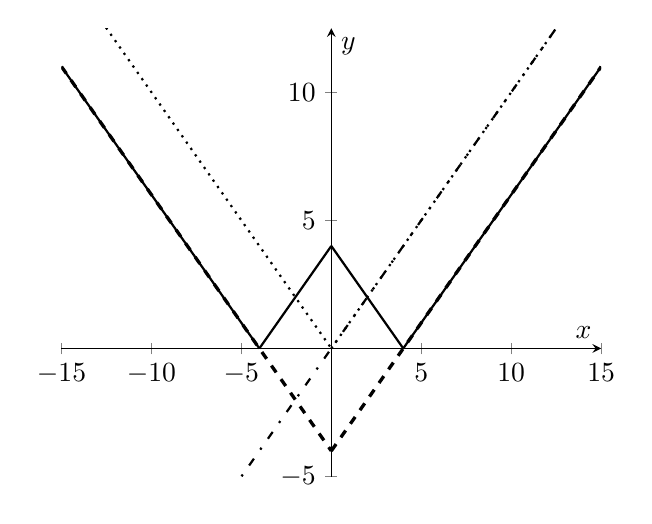
\begin{tikzpicture}
\begin{axis}[axis lines=middle,xlabel=$x$,ylabel=$y$,xmin=-15,xmax=15,ymin=-5,ymax=12.5]

\addplot[thick,color=black,domain=4:15] {x-4};
\addplot[thick,color=black,domain=0:4] {4-x};
\addplot[thick,color=black,domain=-15:-4] {-x-4};
\addplot[thick,color=black,domain=-4:0] {4+x};
\addplot[thick,loosely dashdotted,color=black,domain=-15:15] {x};

\addplot[thick,color=black, dotted,domain=0:15] {x};
\addplot[thick,color=black, dotted,domain=-15:0] {-x};
\addplot[very thick,color=black, dashed,domain=0:15] {x-4};
\addplot[very thick,color=black, dashed,domain=-15:0] {-x-4};
\end{axis}
\end{tikzpicture}
\caption*{Graf funkcije $x\mapsto \abs{|x|-4}$}
\end{subfigure}
\caption{\label{gr1} Grafovi funkcija iz zadatka \ref{exgraph1}} 
\end{figure}
\end{proof}
\newpage
\begin{exercise}
\label{exgraph2}
Nacrtajte graf funkcije $x\mapsto f(x)$, gdje je
\begin{itemize}
\item[a)] $f(x)=\dfrac{x-5}{x+5}$,
\item[b)] $f(x)=e^{|x|}$.
\item[c)] $f(x)=x-\lfloor x\rfloor$.
\end{itemize}
\end{exercise}
\begin{proof}[Rješenje] a) Uočimo da je
$$\dfrac{x-5}{x+5}=\dfrac{x+5-10}{x+5}=1-\dfrac{10}{x+5}.$$
\begin{itemize}
\item Promotrimo graf funkcije $x\mapsto -\dfrac{10}{x}$ (Prikazan točkastom linijom).
\item Tada je graf funkcije $x\mapsto -\dfrac{10}{x-5}$ dobiven translacijom grafa funkcije $x\mapsto \dfrac{10}{x}$ pet jediničnih dužina udesno (Prikazan iscrtkanom linijom).
\item Konačno, graf funkcije $x\mapsto \dfrac{x-5}{x+5}=1-\dfrac{10}{x+5}$ je dobiven translacijom grafa funkcije $x\mapsto -\dfrac{10}{x-5}$ jednu jediničnu dužinu prema gore.
\end{itemize}

b) Uočimo da je
$$e^{|x|}=\begin{cases}
e^x, & x\geq 0, \\
e^{-x}, & x<0.
   \end{cases}$$
Uz ovaj podatak nije teško nacrtati graf ove funkcije. Naime, desno od osi $y$ on će biti identičan grafu funkcije $x\mapsto e^x$, a lijevo od osi $y$ bit će identičan grafu funkcije $x\mapsto e^{-x}$, koji nastaje zrcaljenjem grafa funkcije $x\mapsto e^x$ u odnosu na os $y$. Na slici \ref{gr2} graf funkcije $x\mapsto e^{|x|}$ prikazan je punom linijom. Graf funkcije $x\mapsto e^x$ (odnosno $x\mapsto e^{-x}$), na mjestima gdje se on ne podudara s grafom funkcije $x\mapsto e^{|x|}$, prikazan je točkastom (odnosno iscrtkanom) linijom.
\begin{figure}[ht]
\begin{subfigure}{.5\textwidth}
\centering
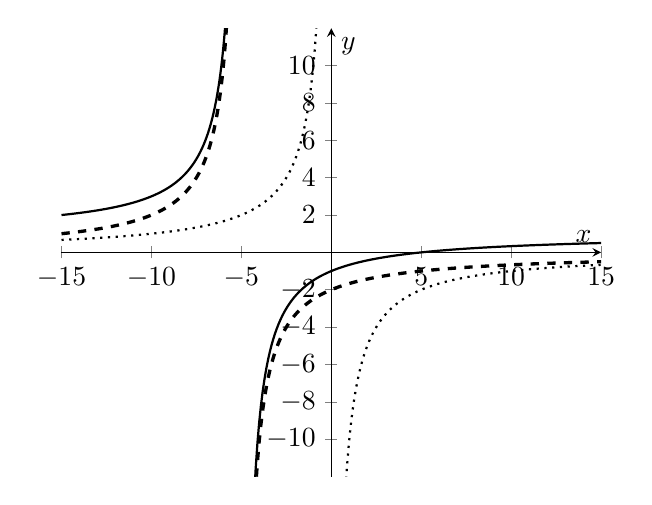
\begin{tikzpicture}
\begin{axis}[axis lines=middle,xlabel=$x$, ytick={-10,-8,-6,-4,-2, 2, 4, 6, 8, 10},ylabel=$y$,xmin=-15,xmax=15,ymin=-12,ymax=12, samples=200]

\addplot[thick,dotted,color=black,domain=-15:-0.5] {-10/x};
\addplot[thick,dotted,color=black,domain=0.5:15] {-10/x};

\addplot[very thick,dashed,color=black,domain=-15:-5.5] {-10/(x+5)};
\addplot[very thick,dashed,color=black,domain=-4.5:15] {-10/(x+5)};

\addplot[thick,color=black,domain=-15:-5.5] {(x-5)/(x+5)};
\addplot[thick,color=black,domain=-4.5:15] {(x-5)/(x+5)};
\end{axis}
\end{tikzpicture}
\caption*{Graf funkcije $x\mapsto \dfrac{x-5}{x+5}$}
\end{subfigure}%
\begin{subfigure}{.5\textwidth}
\centering
\begin{tikzpicture}
\begin{axis}[axis lines=middle,xlabel=$x$,ylabel=$y$,xmin=-4,xmax=4,ymin=-1,ymax=7.5, smooth, samples=200]

\addplot[thick,dotted,color=black,domain=-4:0] {e^x};
\addplot[very thick,dashed,color=black,domain=0:4] {e^(-x)};
\addplot[thick,color=black,domain=0:4] {e^x};
\addplot[thick,color=black,domain=-4:0] {e^(-x)};
\end{axis}
\end{tikzpicture}
\caption*{Graf funkcije $x\mapsto e^{|x|}$ \phantom{$\dfrac{2}{3}$}}
\end{subfigure}
\caption{\label{gr2} Grafovi funkcija iz zadatka \ref{exgraph2} a) i b)}
\end{figure}

c) Na slici \ref{gr3} prikazan je točkastom linijom graf funkcije $x\mapsto x$ i iscrtkanom linijom graf funkcije $x\mapsto -\lfloor x\rfloor$. Prema napomeni \ref{graphrem}, graf funkcije $x\mapsto x-\lfloor x \rfloor$ (prikazan punom linijom) bit će dobiven tako da za proizvoljnu točku $x\in \mathbb{R}$ zbrojimo vrijednosti te dvije funkcije u točki $x$.
\begin{figure}[ht]
\begin{center}
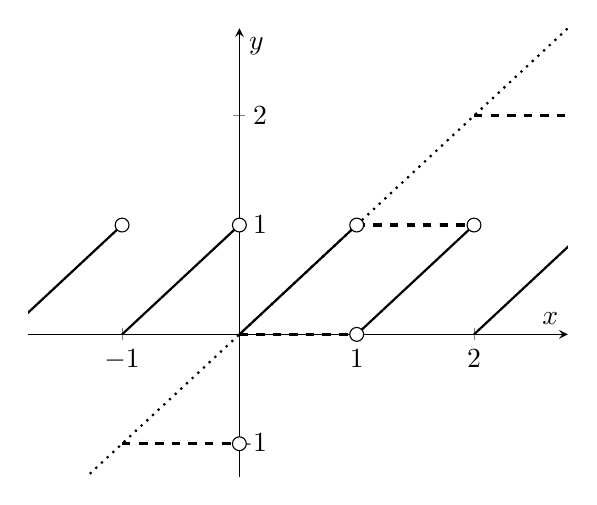
\begin{tikzpicture}
\begin{axis}[axis lines=middle,
    yticklabel style = {xshift=0.55cm},
    xlabel=$x$,ylabel=$y$,xmin=-1.8,xmax=2.8,ymin=-1.3,ymax=2.8]

\addplot[very thick,dashed,color=black,domain=0:1] {0};
\addplot[very thick,dashed,color=black,domain=1:2] {1};
\addplot[very thick,dashed,color=black,domain=2:3] {2};
\addplot[very thick,dashed,color=black,domain=-1:0] {-1};

\addplot[thick,color=black,domain=0:1] {x};
\addplot[thick,color=black,domain=1:2] {x-1};
\addplot[thick,color=black,domain=2:3] {x-2};
\addplot[thick,color=black,domain=-1:0] {x+1};
\addplot[thick,color=black,domain=-2:-1] {x+2};
\addplot[thick,dotted,color=black,domain=-2:3] {x};

\node[circle,draw=black, fill=white, inner sep=0pt,minimum size=5pt] at (1, 1) {};
\node[circle,draw=black, fill=white, inner sep=0pt,minimum size=5pt] at (2, 1) {};
\node[circle,draw=black, fill=white, inner sep=0pt,minimum size=5pt] at (3, 1) {};
\node[circle,draw=black, fill=white, inner sep=0pt,minimum size=5pt] at (0, 1) {};
\node[circle,draw=black, fill=white, inner sep=0pt,minimum size=5pt] at (-1, 1) {};
\node[circle,draw=black, fill=white, inner sep=0pt,minimum size=5pt] at (1, 0) {};
\node[circle,draw=black, fill=white, inner sep=0pt,minimum size=5pt] at (0, -1) {};

\end{axis}
\end{tikzpicture}
\end{center}
\caption{\label{gr3} Graf funkcije iz zadatka \ref{exgraph2} c)}
\end{figure}
\end{proof}
\begin{exercise} Neka je $f : \mathbb{R}\to \mathbb{R}$, $f(x)=\sin{x}$. Graf funkcije $f$ je zrcaljen po osi $y$, zatim je pomaknut za dvije jedinične dužine udesno, a potom je skaliran u odnosu na ishodište, te je koeficijent tog skaliranja (homotetije) $\dfrac{1}{2}$. Graf koje funkcije je novodobiveni skup?
\end{exercise}
\begin{proof}[Rješenje]
Zrcaljenjem dobivamo $x\mapsto -\sin{x}$, pomakom za dvije jedinične dužine udesno dobivamo $x\mapsto -\sin(x-2)$, dilatacijom po $x$ dobivamo $x\mapsto -\sin\left(2x-2\right)$, a dilatacijom po $y$ imamo $x\mapsto \dfrac{1}{2}\sin(2x-2)$. Prema tome novodobiveni skup je graf funkcije $x\mapsto \dfrac{1}{2}\sin(2x-2)$.
\end{proof}

\section{Injekcija, surjekcija i bijekcija. Slika i praslika skupa}

\begin{definition}
Neka su $S$ i $S'$ neprazni skupovi. Funkcija $f : S\to S'$ je
\begin{itemize}
\item \textbf{injekcija} ako za sve $x$, $y\in S$ vrijedi $$f(x)=f(y)\Rightarrow x=y.$$
\item \textbf{surjekcija} ako za sve $y\in S'$ postoji bar jedan $x\in S$ takav da je $f(x)=y$ (tj. vrijedi $S'=\mathcal{R}(f)$).
\item \textbf{bijekcija} ako je injekcija i surjekcija.
\end{itemize}
\end{definition}

\begin{exercise}
Neka je $f : \mathbb{R}^+\to \langle 1, \infty\rangle $ zadana formulom $f(x)=1+\dfrac{1}{x}$. Dokažite da je $f$ bijekcija.
\end{exercise}
\begin{proof}[Rješenje]
Dokažimo da je $f$ injekcija. Neka su $x, y\in \langle 1, \infty\rangle$ takvi da vrijedi $$1+\dfrac{1}{x}=1+\dfrac{1}{y}.$$ Zbog $x$, $y\neq 0$ pojednostavljivanjem i množenjem dobivamo $x=y$. 

Dokažimo da je $f$ surjekcija. Neka je $y\in \langle 1, \infty\rangle$ proizvoljan. Treba dokazati da tada postoji bar jedan $x$ takav da je $$y=1+\dfrac{1}{x}.$$ No ovo je zbog $x\neq 0$ i $y-1\neq 0$ ekvivalentno s $$x=\dfrac{1}{y-1}.$$ Zaista, $\dfrac{1}{y-1}$ je upravo jedan (i jedini) takav $x$.
\end{proof}
\begin{remark}
Lako se vidi sljedeća formulacija definicije bijekcije: $f : S\to S'$ je bijekcija ako i samo ako za svaki $y\in S'$ postoji i jedinstven je $x\in S$ takav da je $y=f(x)$. Prema tome, u prethodnom zadatku prvi dio rješenja je zapravo suvišan.
\end{remark}

\begin{exercise}
Dokažite da je $f : \mathbb{R}\to \langle 0, 1]$ zadana formulom $f(x)=\dfrac{1}{x^2+1}$ surjekcija. Je li i injekcija?
\end{exercise}
\begin{proof}[Rješenje]
Neka je $y\in \langle 0, 1]$. Treba dokazati da postoji bar jedan $x\in \mathbb{R}$ takav da je $$y=\dfrac{1}{1+x^2}.$$ No to je ekvivalentno s $$x^2=\dfrac{1}{y}-1.$$ 
Očito je $x=\sqrt{\dfrac{1}{y}-1}$ jedan $x$ koji zadovoljava tvrdnju. Nadalje, $f$ nije injekcija, jer je $-1\neq 1$ i $f(1)=f(-1)$.
\end{proof}
\begin{exercise} \textbf{}
\label{bijexmp}
\begin{itemize}
\item[a)] Odredite neku bijekciju (ako postoji) s $\mathbb{N}$ u $\mathbb{N}\setminus\{1, 2\}$.
\item[b)] Odredite neku bijekciju (ako postoji) s $\mathbb{N}$ s $[0, 1]$ u $[1, 3]$.
\item[c)] Odredite neku bijekciju (ako postoji) s $\mathbb{N}$ s $[0, 1]$ u $[0, 1\rangle$.
\item[d)] Odredite neku bijekciju (ako postoji) s $\mathbb{R}$ u skup svih funkcija s $\mathbb{R}$ u $\mathbb{R}$ (Taj skup nazivamo $\mathbb{R}^\mathbb{R}$).
\end{itemize}
\end{exercise}
\begin{proof}[Rješenje]
a) Neka je zadana $f : \mathbb{N}\to \mathbb{N}\setminus \{1, 2\}$, $f(n)=n+2$ (Ideja je "pomaknuti" svaki broj za $2$ udesno). Uvjerite se da je ova funkcija zaista bijekcija.

b) Ideja će biti uzeti linearnu funkciju čiji graf prolazi kroz točke $(0, 1)$ i $(1, 3)$ i promotriti njezinu restrikciju na segment $[0, 1]$. Uzmimo $f :[0, 1]\to [1, 3]$, $f(x)=2x+1$. Nije teško pokazati da je ova funkcija zaista bijekcija.

c) Promotrimo funkciju $f : [0, 1]\to [0, 1]$, $f(x)=x$. Ona je očito bijekcija s $[0, 1]$ na $[0, 1]$. Ideja će sada biti nju izmijeniti tako da $f(1)$ bude neki broj iz skupa $[0, 1\rangle$. Doduše, ako to napravimo, funkcija više neće biti injekcija. Zaista, znamo da je $f(f(1))=f(1)$, pa kad bi ona bila injekcija bilo bi $f(1)=1$, što nije točno. Dakle, da bi izbjegli situaciju gdje funkcija poprima dvije jednake vrijednosti, moramo je izmijeniti i za $x=f(1)$. Injektivnost će se opet "pokvariti", ali ćemo tada funkciju moći opet izmijeniti u točki koja "kvari" injektivnost. Ovaj postupak ponavljamo u beskonačnost. Zato ima smisla promotriti npr. funkciju $g : [0, 1]\to [0, 1\rangle$,

$$g(x)=\begin{cases}
x, &\;x\notin S,\\[2pt]
\dfrac{x}{2}, &\; x\in S,
\end{cases}$$
gdje je $S=\left\{\dfrac{1}{2^n} : n\in \mathbb{N}_0\right\}$.

Tvrdimo da je $g$ injekcija. Zaista, neka su $x, y\in [0, 1\rangle$ takvi da je $f(x)=f(y)$. Uočimo da ako je $x\in S$ ako i samo ako je $f(x)\in S$, pa ako je $f(x)=f(y)$, onda su ili $x, y$ oboje u $S$, ili oboje nisu u $S$. U oba slučaja je očigledno $x=y$.

Tvrdimo da je $g$ i surjekcija. Zaista, neka je $y\in [0, 1\rangle$ proizvoljan. Ako je $y\notin S$, onda je $f(y)=y$, ako je $y\in S$, onda postoji $p\in \mathbb{N}$ takav da je $y=\dfrac{1}{2^p}$. No tada je $$g\left(\dfrac{1}{2^{p-1}}\right)=\dfrac{1}{2^p},$$
gdje je $\dfrac{1}{2^{p-1}}\in S$, budući da je $y\neq 1$.

\begin{figure}[ht]
\begin{center}
\begin{tikzpicture}
\begin{axis}[axis lines=middle,   xlabel=$x$,ylabel=$y$,xmin=-0.2,xmax=1.2,ymin=-0.2,ymax=1.2]

\addplot[thick,color=black,domain=0:1] {x};

\node[circle,draw=black, fill=white, inner sep=0pt,minimum size=5pt] at (1, 1) {};
\node[circle,draw=black, fill=white, inner sep=0pt,minimum size=5pt] at (0.5, 0.5) {};
\node[circle,draw=black, fill=white, inner sep=0pt,minimum size=5pt] at (0.25, 0.25) {};
\node[circle,draw=black, fill=white, inner sep=0pt,minimum size=5pt] at (1/8, 1/8) {};
\node[circle,draw=black, fill=white, inner sep=0pt,minimum size=5pt] at (1/16, 1/16) {};
\node[circle,draw=black, fill=white, inner sep=0pt,minimum size=5pt] at (1/32, 1/32) {};
\node[circle,draw=black, fill=white, inner sep=0pt,minimum size=5pt] at (1/64, 1/64) {};

\node[circle,fill,inner sep=2pt] at (axis cs:1, 0.5) {};
\node[circle,fill,inner sep=2pt] at (axis cs:0.5, 0.25) {};
\node[circle,fill,inner sep=2pt] at (axis cs:0.25, 1/8) {};
\node[circle,fill,inner sep=2pt] at (axis cs:1/8, 1/16) {};
\node[circle,fill,inner sep=2pt] at (axis cs:1/16, 1/32) {};
\node[circle,fill,inner sep=2pt] at (axis cs:1/32, 1/64) {};
\node[circle,fill,inner sep=2pt] at (axis cs:1/64, 1/128) {};
\end{axis}
\end{tikzpicture}
\end{center}
\caption{\label{exbij} Graf funkcije iz zadatka \ref{bijexmp} c)}
\end{figure}

d) Tvrdimo da takva bijekcija ne postoji. Zaista, pretpostavimo da postoji bijekcija $f : \mathbb{R}\to \mathbb{R}^{\mathbb{R}}$. Tada je ona surjekcija, što znači da za svaki $y\in \mathbb{R}^{\mathbb{R}}$ postoji $x_0\in \mathbb{R}$ takav da je $f(x_0)=y$, što povlači da je $f(x_0)(x_0)=y(x_0)$. No to očito ne vrijedi ako promotrimo funkciju $y : \mathbb{R}\to \mathbb{R}$ definiranu formulom $y(x)=f(x)(x)+1$, za svaki $x\in \mathbb{R}$.
\end{proof}
\begin{definition}
\label{monotonic}
Neka je $S\subseteq \mathbb{R}$ neprazan, te $x, y\in S$. Kažemo da je funkcija $f : S\to \mathbb{R}$ \textbf{monotono rastuća} (kraće: rastuća) ako vrijedi $x<y\Rightarrow f(x)\leq f(y)$, \textbf{strogo rastuća} ako vrijedi $x<y\Rightarrow f(x)<f(y)$, \textbf{monotono padajuća} (kraće: padajuća) ako vrijedi $x<y\Rightarrow f(x)\geq f(y)$, \textbf{strogo padajuća} ako vrijedi $x<y\Rightarrow f(x)>f(y)$.
\end{definition}
\begin{remark}
Neka su $S, S'\subseteq \mathbb{R}$ neprazni i neka je zadana $f : S\to S'$. Ako je $f$ strogo monotona (tj. strogo rastuća ili strogo padajuća), ona je injekcija.
\end{remark}
\begin{exercise}
Zadana je $f : \mathbb{R}\to \mathbb{R}$, $f(x)=e^{-2x}$. Dokažite da je $f$ injekcija koristeći se činjenicom da je strogo monotona.
\end{exercise}
\begin{proof}[Rješenje]
Iz grafa se vidi da je $f$ strogo padajuća. 
\begin{figure}[ht]
\begin{center}
\begin{tikzpicture}
\begin{axis}[axis lines=middle, xlabel=$x$,ylabel=$y$,xmin=-1.8,xmax=3.2,ymin=-0.5,ymax=3.8, samples=150]


\addplot[thick,color=black,domain=-1:3.3] {e^(-2*x)};

\end{axis}
\end{tikzpicture}
\end{center}
\caption{\label{grexp} Graf funkcije $x\mapsto e^{-2x}$}
\end{figure}

Zaista, treba pokazati da za sve $x, y\in \mathbb{R}$ vrijedi
\begin{gather}
\label{ineq1}
x<y\Rightarrow e^{-2y}<e^{-2x}.
\end{gather}
Uočimo da, kako je $e^x\geq 0$ za sve $x\in \mathbb{R}$ i $x\mapsto x^2$ i $x\mapsto \sqrt{x}$ strogo rastuće funkcije, vrijedi
$$e^{-2y}<e^{-2x}\Leftrightarrow \dfrac{1}{\left(e^{y}\right)^2}<\dfrac{1}{\left(e^{x}\right)^2}\Leftrightarrow \left(e^{x}\right)^2<\left(e^{y}\right)^2\Leftrightarrow e^x<e^y.$$
Dakle (\ref{ineq1}) je ekvivalentno tvrdnji da za sve $x,y\in \mathbb{R}$ vrijedi $$x<y\Rightarrow e^x<e^y,$$
što vrijedi, jer je funkcija $x\mapsto e^x$ strogo rastuća.
\end{proof}
\begin{definition}
Neka je $S\subseteq \mathbb{R}$ neprazan. Kažemo da je $f : S\to \mathbb{R}$ injekcija, odnosno surjekcija na nekom podskupu od $S'\subseteq S$ ako je $f|_{S'}$ injekcija, odnosno surjekcija. Također, kažemo da je $f$ strogo rastuća (padajuća) na $S'$ ako je $f|_{S'}$ strogo rastuća (padajuća) na $S$.
\end{definition}
\begin{exercise}
Dokažite da je funkcija $f : \mathbb{R}\to \mathbb{R}$, $f(x)=x\sqrt{1+x^2}$ injekcija.
\end{exercise}
\begin{proof}[Rješenje]
Iz grafa funkcije $f$ vidi se da je ona strogo rastuća.
\begin{figure}[ht]
\begin{center}
\begin{tikzpicture}
\begin{axis}[axis lines=middle, xlabel=$x$,ylabel=$y$,xmin=-6.2,xmax=6.2,ymin=-8.2,ymax=8.2, samples=150]


\addplot[thick,color=black,domain=-4.3:4.3] {x*sqrt(1+x^2)};

\end{axis}
\end{tikzpicture}
\end{center}
\caption{\label{gr4} Graf funkcije $x\mapsto x\sqrt{1+x^2}$}
\end{figure}

Dokažimo to! Uočimo da je $x\mapsto \sqrt{1+x^2}$ strogo rastuća na $[0, \infty\rangle$ i strogo padajuća na $\langle-\infty, 0]$. Zaista, za sve $x, y\geq 0$ vrijedi
$$x<y\Rightarrow x^2<y^2\Rightarrow 1+x^2<1+y^2\Rightarrow \sqrt{1+x^2}<\sqrt{1+y^2}.$$
Analogno dobivamo i da $f$ strogo pada na $\langle-\infty, 0]$. Neka su sada $x, y\in \mathbb{R}$ takvi da je $x<y$. Razlikujemo tri slučaja.

\begin{itemize}
\item[a)] $x\leq 0$, $y>0$,
\item[b)] $x, y\geq 0$,
\item[c)] $x, y\leq 0$.
\end{itemize}

U slučaju a), $f(x)<f(y)$ je trivijalno, jer je $f(x)\leq 0$ i $f(y)>0$. 

U slučaju b) imamo $\sqrt{1+x^2}<\sqrt{1+y^2}$, pa množenjem s nejednakosti $x<y$ dobivamo $x\sqrt{1+x^2}<y\sqrt{1+y^2}$ (Uočimo da ovo smijemo zaključiti, jer su ili $x, y>0$, pa primjenjujemo napomenu \ref{10}, ili je $x=0$ i $y>0$, pa je tvrdnja očigledna).

U slučaju c) imamo $-y<-x$ i $-y, -x\geq 0$, pa iz $b)$ slijedi $$-y\sqrt{1+(-y)^2}<-x\sqrt{1+(-x)^2}.$$ Tvrdnja sada slijedi množenjem s $-1$ i korištenjem svojstva parnosti funkcije $x\mapsto x^2$, tj. činjenice da je $(-x)^2=x^2$ za sve $x\in \mathbb{R}$.
\end{proof}
Slijede zadatci gdje određujemo sliku $\mathcal{R}(f)$ zadane funkcije $f$.

\begin{exercise}
\label{eximg}
Neka je $f : \mathbb{R}\to \mathbb{R}$ zadana formulom
$$f(x)=\begin{cases}
2x, & x\neq 3, \\
0, & x=3.
   \end{cases}$$
Odredite $\mathcal{R}(f)$.
\end{exercise}
\begin{proof}[Rješenje]
Iz grafa funkcije $f$ vidi se da je $\mathcal{R}(f)=\mathbb{R}\setminus \{6\}$. Zaista, dokazat ćemo da je $$\mathcal{R}(f)\subseteq \mathbb{R}\setminus \{6\}\;\;\;\;\text{i}\;\;\;\;\mathbb{R}\setminus \{6\}\subseteq \mathcal{R}(f).$$
Neka je $y\in \mathbb{R}$ takav da je $y\neq 6$. Tvrdimo da tada postoji $x\in \mathbb{R}$ takav da je $f(x)=y$. Zaista, uzmimo $x=\dfrac{y}{2}$. Tada je $f\left(\dfrac{y}{2}\right)=y$ ako je $y\neq 0$, a isto vrijedi i za $y=0$, jer je $f(0)=0$.
\begin{figure}[ht]
\begin{center}
\begin{tikzpicture}
\begin{axis}[axis lines=middle,   xlabel=$x$,ylabel=$y$,xmin=-8.2,xmax=8.2,ymin=-8.2,ymax=8.2]

\addplot[thick,color=black,domain=-4.5:4.5] {2*x};

\node[circle,draw=black, fill=white, inner sep=0pt,minimum size=5pt] at (3, 6) {};

\node[circle,fill,inner sep=2pt] at (axis cs:3, 0) {};

\end{axis}
\end{tikzpicture}
\end{center}
\caption{\label{exim1} Graf funkcije iz zadatka \ref{eximg}}
\end{figure}

S druge strane, neka je $y\in \mathcal{R}(f)$. Tvrdimo da je $y\neq 6$. Zaista, postoji $x\in \mathbb{R}$ takav da je $y=f(x)$. Ako je $x<3$, onda je $y=2x<6$, te analogno $y=2x>6$ za $x>3$. Za $x=3$ imamo $y=0\neq 6$, pa je tvrdnja dokazana.
\end{proof}
\newpage
\begin{exercise}
\label{eximg2}
Zadana je funkcija $f : \mathbb{R}\to \mathbb{R}$, $f(x)=\dfrac{1}{x^2+5x+8}$. Odredite $\mathcal{R}(f)$.
\end{exercise}
\begin{proof}[Rješenje]
Po definiciji, $\mathcal{R}(f)$ je skup svih $k\in \mathbb{R}$ za koje postoji $x\in \mathbb{R}$ takav da je
\begin{gather}
\label{31}
\dfrac{1}{x^2+5x+8}=k.
\end{gather}
Jednakost (\ref{31}) je ekvivalentna jednakosti
$$kx^2+5kx+8k-1=0.$$
Za $k=0$ imamo $-1=0$, što ne vrijedi. Dakle, $0\notin \mathcal{R}(f)$. Ako je $k\neq 0$, onda imamo kvadratnu jednadžbu, za koju znamo da ima rješenja ako i samo ako je
$$25k^2-4k(8k-1)\geq 0,\text{ odnosno } 4k-7k^2\geq 0.$$
Rješenje kvadratne nejednadžbe $4k-7k^2\geq 0$ je $\left[0, \dfrac{4}{7}\right]$, ali kako je $k\neq 0$, zaključujemo da postoji $x\in \mathbb{R}$ takav da vrijedi (\ref{31}) ako i samo ako je $k\in \left\langle 0, \dfrac{4}{7}\right]$. Dakle, $\mathcal{R}(f)=\left\langle 0, \dfrac{4}{7}\right]$.
\begin{figure}[ht]
\begin{center}
\begin{tikzpicture}
\begin{axis}[axis lines=middle,   xlabel=$x$,ylabel=$y$,xmin=-6.2,xmax=4.2,ymin=-0.2,ymax=2.2, samples=150]

\addplot[thick,color=black,domain=-6.2:4.5] {1/(x^2+5*x+8)};

\end{axis}
\end{tikzpicture}
\end{center}
\caption{\label{exim2} Graf funkcije iz zadatka \ref{eximg2}}
\end{figure}
\end{proof}

\begin{remark}
Uočimo da iz slike \ref{exim2} nije odmah jasno čemu bi slika funkcije mogla biti jednaka. Dakle, osim radi matematičke strogosti, ponekad se određivanje slike po definiciji isplati upravo zato što daje točno, a ne približno, rješenje.
\end{remark}
\newpage
\begin{definition}
Neka je zadana $f : A\to B$ i $S\subseteq A$, te $T\subseteq B$. Tada je \textbf{slika skupa} $S$ u odnosu na $f$ skup $f(S)=\{f(x) : x\in S\}$, a \textbf{praslika skupa} $T$ u odnosu na $f$ je skup $f^{-1}(T)=\{a\in A : f(a)\in T\}$. Dogovorno uzimamo $f(\emptyset)=\emptyset$ i $f^{-1}(\emptyset)=\emptyset$.
\end{definition}
\begin{definition}
Neka je $S\subseteq \mathbb{R}$ neprazan. Kažemo da je $f : S\to \mathbb{R}$ injekcija, odnosno surjekcija na nekom podskupu od $S'\subseteq S$ ako je $f|_{S'}$ injekcija, odnosno surjekcija. Također, kažemo da je $f$ strogo rastuća (padajuća) na $S'$ ako je $f|_{S'}$ strogo rastuća (padajuća) na $S$.
\end{definition}
\begin{exercise}
Zadana je $f : \mathbb{R}\to \mathbb{R}$, $f(x)=x^2+2x-1$. Odredite $f\left(\left[1, 2\right]\right)$ i $f^{-1}\left(\left[2, 7\right]\right)$.
\end{exercise}
\begin{proof}[Rješenje]
Iz grafa vidimo da je $f\left(\left[1, 2\right]\right)=[2, 7]$, te $f^{-1}\left(\left[2, 7\right]\right)=[-4, -3]\cup [1, 2]$.
\begin{figure}[ht]
\begin{subfigure}{.5\textwidth}
\centering
\begin{tikzpicture}
\begin{axis}[axis lines=middle,xlabel=$x$,ylabel=$y$,xmin=-4.1,xmax=4,ymin=-2.1,ymax=7.9, smooth]

\node[inner sep=2pt] at (axis cs:1,0) {\textbf{[}};
\node at (axis cs:2,0) {\textbf{]}};

\node[rotate=90] at (axis cs:0,2) {\textbf{[}};
\node[rotate=90] at (axis cs:0,7) {\textbf{]}};

\addplot[thick,color=black,domain=-4.5:4] {x^2+2*x-1};
\addplot[thick,dashed,color=black,domain=0:1] {2};
\addplot[thick,dashed,color=black,domain=0:2] {7};
\draw[dashed] (axis cs:1,0) -- (axis cs:1,2);
\draw[dashed] (axis cs:2,0) -- (axis cs:2,7);
\draw [-{Stealth[slant=0]}] (axis cs:1.25, 0.25)--(axis cs:1.25, 1.75);
\draw [-{Stealth[slant=0]}] (axis cs:1.5, 0.25)--(axis cs:1.5, 1.75);
\draw [-{Stealth[slant=0]}] (axis cs:1.75, 0.25)--(axis cs:1.75, 1.75);
\draw [-{Stealth[slant=0]}] (axis cs:0.9, 2.9)--(axis cs:0.1,2.9);
\draw [-{Stealth[slant=0]}] (axis cs:0.9, 5.8)--(axis cs:0.1,5.8);

\draw [-{Stealth[slant=0]}] (axis cs:0.9, 4.35)--(axis cs:0.1,4.35);
\end{axis}
\end{tikzpicture}
\caption{\label{exim3} Slika skupa $[1, 2]$ u odnosu na $f$}
\end{subfigure}%
\begin{subfigure}{.5\textwidth}
\centering
\begin{tikzpicture}
\begin{axis}[axis lines=middle,xlabel=$x$,ylabel=$y$,xmin=-4.1,xmax=4,ymin=-2.1,ymax=7.9, smooth]

\node[inner sep=2pt] at (axis cs:1,0) {\textbf{[}};
\node at (axis cs:2,0) {\textbf{]}};

\node[inner sep=2pt] at (axis cs:-4,0) {\textbf{[}};
\node at (axis cs:-3,0) {\textbf{]}};

\node[rotate=90] at (axis cs:0,2) {\textbf{[}};
\node[rotate=90] at (axis cs:0,7) {\textbf{]}};

\addplot[thick,color=black,domain=-4.5:4] {x^2+2*x-1};
\addplot[thick,dashed,color=black,domain=-3:1] {2};
\addplot[thick,dashed,color=black,domain=-4:2] {7};

\addplot[thick,color=black,domain=-4.5:4] {x^2+2*x-1};
\addplot[thick,dashed,color=black,domain=0:1] {2};
\addplot[thick,dashed,color=black,domain=0:2] {7};
\draw[dashed] (axis cs:1,0) -- (axis cs:1,2);
\draw[dashed] (axis cs:2,0) -- (axis cs:2,7);
\draw[dashed] (axis cs:-3,0) -- (axis cs:-3,2);
\draw[dashed] (axis cs:-4,0) -- (axis cs:-4,7);
\draw [-{Stealth[slant=0]}] (axis cs:1.25, 1.75)--(axis cs:1.25, 0.25);
\draw [-{Stealth[slant=0]}] (axis cs:1.5, 1.75)--(axis cs:1.5, 0.25);
\draw [-{Stealth[slant=0]}] (axis cs:1.75, 1.75)--(axis cs:1.75, 0.25);
\draw [-{Stealth[slant=0]}] (axis cs:0.1,2.9)--(axis cs:0.9, 2.9);
\draw [-{Stealth[slant=0]}] (axis cs:0.1,5.8)--(axis cs:0.9, 5.8);
\draw [-{Stealth[slant=0]}] (axis cs:0.1,4.35)--(axis cs:0.9, 4.35);

\draw [-{Stealth[slant=0]}] (axis cs:-0.1,2.9)--(axis cs:-0.9, 2.9);
\draw [-{Stealth[slant=0]}] (axis cs:-0.1,5.8)--(axis cs:-0.9, 5.8);
\draw [-{Stealth[slant=0]}] (axis cs:-0.1,4.35)--(axis cs:-0.9, 4.35);

\draw [-{Stealth[slant=0]}] (axis cs:-3.25, 1.75)--(axis cs:-3.25, 0.25);
\draw [-{Stealth[slant=0]}] (axis cs:-3.5, 1.75)--(axis cs:-3.5, 0.25);
\draw [-{Stealth[slant=0]}] (axis cs:-3.75, 1.75)--(axis cs:-3.75, 0.25);
\end{axis}
\end{tikzpicture}
\caption{\label{exim4} Praslika skupa $[2, 7]$ u odnosu na $f$}
\end{subfigure}
\caption{Graf funkcije $x\mapsto x^2+2x-1$}
\end{figure}

Dokažimo da je $f^{-1}\left(\left[2, 7\right]\right)=[-4, -3]\cup [1, 2]$. Trebamo pronaći sve $x\in \mathbb{R}$ takve da je $f(x)\in [2, 7]$, tj. trebamo riješiti sustav 
$$\begin{cases}
x^2+2x-1\geq 2,\\
x^2+2x-1\leq 7,
\end{cases}$$
Vrijedi
$$x^2+2x-1\geq 2\Leftrightarrow x^2+2x-3\geq 0\Leftrightarrow (x-1)(x+3)\geq 0\Leftrightarrow x\in \langle-\infty, -3]\cup [1,\infty\rangle.$$
Analogno dobivamo da je $x^2+2x-1\leq 7$ ako i samo ako je $x\in [-4, 2]$. Rješenje sustava je presjek ta dva skupa, što daje tvrdnju.

Dokažimo sada da je $f\left([1, 2]\right)=[2, 7]$. Neka je $y\in f\left([1, 2]\right)$ proizvoljan. Po definiciji, postoji $x\in [1, 2]$ za kojeg vrijedi
\begin{gather}
\label{33}
y=x^2+2x-1.
\end{gather}
Izrazimo li iz ove jednakosti $x$ (Tako da je tretiramo kao kvadratnu jednadžbu po $x$), dobivamo da je (\ref{33}) ekvivalentno tvrdnji
\begin{gather}
\label{32}
x=-1+\sqrt{y+2}\;\;\;\text{ ili }\;\;\;x=-1-\sqrt{y+2}. 
\end{gather}
Kako je $-1-\sqrt{y+2}\leq -1$, kad bi vrijedilo $x=-1-\sqrt{y+2}$, bilo bi $x\notin [1, 2]$, suprotno pretpostavci. Zaključujemo da je (\ref{32}) ekvivalentno tvrdnji $x=-1+\sqrt{y+2}$. 

Sada moramo ispitati nužne i dovoljne uvjete da vrijedi $$-1+\sqrt{y+2}\in [1, 2],$$
tj. trebamo riješiti sustav
$$\begin{cases}
-1+\sqrt{y+2}\geq 1,\\
-1+\sqrt{y+2}\leq 2,
\end{cases}$$
Imamo
$$-1+\sqrt{y+2}\geq 1\Leftrightarrow \sqrt{y+2}\geq 2\Leftrightarrow y+2\geq 4\Leftrightarrow y\geq 2,$$
te se analogno dobije $y\leq 7$ iz drugog uvjeta. Dakle, pokazali smo da vrijedi $y\in f([1, 2])$ ako i samo ako vrijedi $y\in [2, 7]$, pa je tvrdnja dokazana.
\end{proof}
\begin{remark}
Vidimo da što imamo "kompliciranije" funkcije, to je određivanje slike zapravo teže. Zapravo, često je jedna od najbitnijih tvrdnji o kojoj ovisi slika funkcije ta da $f$ poprima svaku međuvrijednost, da je slika funkcije zaista interval, odnosno da u sebi nema "rupe". Ovo je jedan od mnogih razloga zašto se pokazuje korisnim proučavanje \textit{neprekidnih funkcija} na nekom skupu, što su, neformalno, funkcije čiji graf nema prekide na nekom skupu, tj. izgleda kao da je nacrtan u jednom potezu. Kasnije na kolegiju ćete vidjeti da sve funkcije neprekidne na segmentu imaju ovo svojstvo, i ako je neka funkcija neprekidna na nekom segmentu (a ovo svojstvo zadovoljava vrlo velika klasa funkcija) onda koristeći ovo svojstvo relativno lako možemo matematički precizno odrediti sliku. Time ćemo se još baviti u poglavlju o neprekidnosti.
\end{remark}
\newpage
\begin{remark}
\label{imset}
Neka su $X,Y\subseteq \mathbb{R}$ neprazni. Za funkciju $f : X\to Y$ i neprazne $A, B\subseteq X$, $C, D\subseteq Y$ vrijedi
\begin{itemize}
\item $f(A\cup B)=f(A)\cup f(B)$, \hspace{0.5cm} $f^{-1}(C\cup D)=f^{-1}(C)\cup f^{-1}(D)$,
\item $f(A\cap B)\subseteq f(A)\cap f(B)$, \hspace{0.5cm} $f^{-1}(C\cap D)=f^{-1}(C)\cap f^{-1}(D)$,
\item $f\left(A\setminus B\right)\supseteq f(A)\setminus f(B)$, \hspace{0.5cm} $f^{-1}\left(C\setminus D\right)=f^{-1}(C)\setminus f^{-1}(D)$,
\item $A\subseteq f^{-1}(f(A))$.
\end{itemize}
\end{remark}
\begin{exercise}
Neka su $A, B, X, Y$ i $f$ isti kao i u napomeni \ref{imset}. Dokažite $f(A\cup B)=f(A)\cup f(B)$.
\end{exercise}
\begin{proof}
Neka je $y\in f(A\cup B)$. Tada postoji $x\in A\cup B$ takav da je $y=f(x)$. No ovo vrijedi ako i samo ako postoji $x\in A$ takav da je $y=f(x)$, ili postoji $x\in B$ takav da je $y=f(x)$, što zapravo znači $y\in f(A)\cup f(B)$.
\end{proof}
\begin{exercise}
Dokažite da je funkcija $f : \mathbb{R} \to \langle -1, 1\rangle$ zadana formulom $f(x)=\dfrac{x}{1+|x|}$ bijekcija.
\end{exercise}
\begin{proof}[Rješenje]
Dokažimo prvo injektivnost. Neka su $x$ i $y$ proizvoljni i neka vrijedi $f(x)=f(y)$, tj.
$$\dfrac{x}{1+|x|}=\dfrac{y}{1+|y|}\Leftrightarrow x\left(1+|y|\right)=y\left(1+|x|\right).$$
Kako je ovaj izraz simetričan, odnosno možemo zamijeniti mjesta varijablama $x$ i $y$ bez promjene smisla jednakosti, bez smanjenja općenitosti možemo uzeti da je $x\leq y$. Sada imamo tri slučaja: 
\begin{itemize}
\item $y\geq 0$ i $x\geq 0$, 
\item $y\leq 0$ i $x\leq 0$, 
\item $y\geq 0$ i $x\leq 0$.
\end{itemize}
U prvom slučaju imamo 
$$x(1+y)=y(1+x),$$
što je ekvivalentno tvrdnji $x=y$. Drugi slučaj je analogan. 

Treći slučaj je nešto zahtjevniji. Ako je $y\geq 0$ i $x\leq 0$, onda je $|y|=y$ i $|x|=-x$. No to povlači da za sve tako odabrane $x$ i $y$ vrijedi $$x(1+y)=y(1-x),\;\;\;\text{odnosno}\;\;\;x+2xy-y=0.$$ Rješavanjem po $y$ dobivamo
$$y=-\dfrac{x}{2x-1}.$$
Sada iz $x\leq 0$ slijedi $2x-1<0$, pa iz toga i iz $y\geq 0$ imamo
$$y=-\dfrac{x}{2x-1}\geq 0\Leftrightarrow -x\leq 0\Leftrightarrow x\geq 0.$$
Sada $x\leq 0$ i $x\geq 0$ povlači $x=0$ i posljedično $y=0$, pa očito vrijedi $x=y$. 

Dokažimo sada surjektivnost. Zapravo treba pokazati da je $f(\mathbb{R})=\langle -1, 1\rangle$. To će biti najlakše korištenjem napomene \ref{imset}. Znamo da je 
$$f(\mathbb{R})=f\left(\langle -\infty, 0]\cup [0,\infty\rangle\right)=f\left(\langle -\infty, 0]\right)\cup f\left([0,\infty\rangle\right)$$
Kako za $g=f | _{[0, \infty\rangle}$ vrijedi $g(x)=\dfrac{x}{1+x}$ i vrijedi $f\left([0,\infty\rangle\right)=g\left([0,\infty\rangle\right)=\mathcal{R}(g)$, slijedi da je $f\left([0,\infty\rangle\right)=[0, 1\rangle$ i $f\left(\langle -\infty, 0]\right)=\langle -1, 0]$ (Uvjerite se u to!). Sada je $f(\mathbb{R})=\langle -1, 1\rangle$ i tvrdnja je dokazana.
\end{proof}
\section{Kompozicija funkcija. Inverzna funkcija}
\begin{definition}
Zadane su funkcije $f : A\to B$ i $g : C\to D$. Ako je $\mathcal{R}(f)\subseteq \mathcal{D}(g)$, onda je funkcija $h : A\to D$, $h(x)=g(f(x))$ \textbf{kompozicija funkcija} $f$ i $g$, i označavamo je s $h=g\circ f$.
\end{definition}
\begin{exercise} \textbf{}
\begin{itemize}
\item[a)] Zadana je $f : \mathbb{R}\to \mathbb{R}$, $f(x)=\sqrt{1+x^2}$. Prikažite $f$ kao kompoziciju jednostavnijih funkcija.
\item[b)] Zadana je $f : \mathbb{R}\to \mathbb{R}$, $f(x)=2x^2+4x$. Dokažite da postoje $a, b\in \mathbb{R}$ takvi da se $f$ može prikazati kao kompozicija funkcija $$f,g_a,h_b : \mathbb{R}\to \mathbb{R},\;f(x)=x^2,\; g_a(x)=x+a,\; h_b(x)=bx.$$
\end{itemize}
\end{exercise}
\begin{proof}[Rješenje]
a) Definiramo $f_1, f_2, f_3 : \mathbb{R}\to \mathbb{R}$ formulama $f_1(x)=x^2$, $f_2(x)=1+x$, $f_3(x)=\sqrt{x}$. Tada je očito $f=f_3\circ f_2\circ f_1$.

b) Uočimo da je
$$2x^2+4x=2(x+1)^2-2.$$
Odavde direktno slijedi $f=g_1\circ f\circ g_{-1}\circ h_2.$
\end{proof}
\begin{remark} Vrijedi:
\begin{itemize}
\item Neka su $S_1, S_2, S_3$ i $S$ neprazni. Zadane su $f_1 : S_1 \to S$, $f_2 : S_2\to S$ i $f_3 : S_3\to S$ za koje je $\mathcal{R}(f_1)\subseteq S_2$ i $\mathcal{R}(f_2)\subseteq S_3$. Tada su dobro definirane funkcije $(f_3\circ f_2)\circ f_1$, $f_3\circ (f_2\circ f_1)$ i vrijedi $(f_3\circ f_2)\circ f_1=f_3\circ (f_2\circ f_1).$
\item Neka su $A, B, C, D\subseteq \mathbb{R}$ neprazni i neka su zadane injekcije $f : A\to B$ i $g : C\to D$ takve da je $\mathcal{R}(f)\subseteq \mathcal{D}(g)$. Tada je i $g\circ f$ injekcija.
\item Neka su $A, B, C\subseteq \mathbb{R}$ neprazni i neka su zadane surjekcije $f : A\to B$ i $g : B\to C$. Tada je i $g\circ f$ surjekcija.
\item Neka su $A, B, C\subseteq \mathbb{R}$ neprazni i neka su zadane bijekcije $f : A\to B$ i $g : B\to C$. Tada je i $g\circ f$ bijekcija.
\end{itemize}
\end{remark}

\begin{exercise}
Dokažite da je $f : [0, 1\rangle\to \mathbb{R}$ zadana formulom $f(x)=x^4+5x^2+6$ injekcija.
\end{exercise}
\begin{proof}[Rješenje]
Neka je $g_1 : [0, 1\rangle\to \mathbb{R}$ zadana formulom $g_1(x)=x^2$, a $g_2 : \mathbb{R}\to \mathbb{R}$ zadana formulom $g_2(x)=x^2+5x+6$. Kako je $\mathcal{R}(g_1)=[0, 1\rangle$ (Provjerite to, računski ili pomoću grafa!) i $\mathcal{D}(g_2)=[0, \infty\rangle$, te očito vrijedi $[0, 1\rangle\subseteq \mathbb{R}$, kompozicija $g_2\circ g_1$ je definirana. Očito je $g_1$ strogo rastuća, ali i $g_2$ je također strogo rastuća, a to se (s trenutnim teorijskim aparatom) najlakše pokazuje na sljedeći način. Neka su $x, y\in \mathbb{R}$ takvi da je $0\leq x<y$. Tada je očito $x+\dfrac{5}{2}<y+\dfrac{5}{2}$, a iz $x\geq 0$ i $y>0$ slijedi $$\left(x+\dfrac{5}{2}\right)^2<\left(y+\dfrac{5}{2}\right)^2.$$ Sada vrijedi
$$x^2+5x+6=\left(x+\dfrac{5}{2}\right)^2-\dfrac{1}{4}<\left(y+\dfrac{5}{2}\right)^2-\dfrac{1}{4}$$
i tvrdnja je dokazana. To znači da su $g_1$ i $g_2$ injekcije, pa je i kompozicija $g_2\circ g_1=f$ također injekcija, čime smo dokazali početnu tvrdnju.
\end{proof}
\begin{exercise}
Neka je $k\in \mathbb{N}$ proizvoljan. Uvedimo oznaku: $\mathbb{N}_k:=\{1, 2,\dots, k\}$. Dokažite: Ako je $f : \mathbb{N}_k\to \mathbb{N}_k$ injekcija, ona je i surjekcija.
\end{exercise}
\begin{proof}[Rješenje]
Tvrdnju dokazujemo indukcijom po $k$. Za $k=1$ je jedina funkcija koja ima smisla ona koja preslikava $1$ u $1$, a ta je očito i injekcija i surjekcija.

Pretpostavimo da za $k\in \mathbb{N}$ vrijedi da je svaka funkcija  i dokažimo da je injekcija $f : \mathbb{N}_k\to \mathbb{N}_k$ injekcija, ona je i surjekcija. Neka je $f : \mathbb{N}_{k+1}\to \mathbb{N}_{k+1}$ injekcija. Tada je $f|_{\mathbb{N}_k}$ također injekcija. 

Pretpostavimo da je $f(k+1)=k+1$, Tada je dobro definirana funkcija $g : \mathbb{N}_k\to \mathbb{N}_k$, $g(n)=f(n)$ za sve $n\in \mathbb{N}_k$. Ona je očito injekcija, pa je po pretpostavci indukcije i surjekcija. Sada uočimo da je
$$f(x)=\begin{cases}
g(x), &\;x\in \mathbb{N}_k,\\
k+1, &\; x=k+1,
\end{cases}$$
i odavde se vidi da je $f$ surjekcija. Zaista, ako je $y\in \mathbb {N}_k$, onda postoji $x\in \mathbb{N}_k$ takav da je $g(x)=f(x)=y$, a ako je $y=k+1$, onda je očito $f(k+1)=k+1$.

Preostaje dokazati tvrdnju u slučaju kad je $f(k+1)=i_0\in \mathbb{N}_k$. Tvrdimo da postoji $j_0\in \mathbb{N}_k$ takav da je $f(j_0)=k+1$. Zaista, ako takav $j_0$ ne postoji, onda je dobro definirana funkcija $f' : \mathbb{N}_k\to \mathbb{N}_k$, $f'(x)=f(x)$, za sve $x\in \mathbb{N}_k$. Očito je $f'$ injekcija, pa je po pretpostavci indukcije i surjekcija, pa postoji $i_1\in \mathbb{N}_k$ takav da je $f(i_1)=i_0=f(k+1)$, dakle $i_1=k+1$, što je nemoguće.

Sada je ideja sljedeća -- za funkciju $f$ vrijedi $f(k+1)=i_0$ i postoji $j_0\in \mathbb{N}_k$ takav da je $f(j_0)=k+1$, pa promotrimo funkciju $F : \mathbb{N}_{k+1}\to \mathbb{N}_{k+1}$,
$$F(x)=\begin{cases}
f(x), &\;x\notin\{j_0, k+1\},\\
k+1, &\; x=k+1,\\
i_0, &\; x=j_0,
\end{cases}$$
i pokažimo da je ona injekcija. U tu svrhu definiramo funkciju $h : \mathbb{N}_{k+1}\to \mathbb{N}_{k+1}$,
$$h(x)=\begin{cases}
x, &\;x\notin\{i_0, k+1\},\\
k+1, &\; x=i_0,\\
i_0, &\; x=k+1.
\end{cases}$$
Nije teško provjeriti da je $h$ injekcija (Dokaz je vrlo sličan onome u zadatku \ref{bijexmp} c)). Pokažimo da je $F=h\circ f$. Zaista, vrijedi 
\begin{gather*}
(h\circ f)(k+1)=h\left(f(k+1)\right)=h(i_0)=k+1=F(k+1),\\
(h\circ f)(j_0)=h\left(f(j_0)\right)=h(k+1)=i_0=F(j_0).
\end{gather*}
Ako je $x\neq j_0$ i $x\neq k+1$, onda je $f(x)\neq k+1$ i $f(x)\neq i_0$, pa za $x\in \mathbb{N}\setminus\{j_0, k+1\}$ vrijedi $$(h\circ f)(x)=h\left(f(x)\right)=f(x)=F(x),$$
čime smo pokazali da je $F=h\circ f$. Zaključujemo da je $F$ injekcija, kao kompozicija injekcija. Sada surjektivnost slijedi iz prvog dijela dokaza.
\end{proof}
\begin{exercise}
\label{compim}
Neka su $f : X\to Y$ i $g : A\to B$ funkcije takve da je $\mathcal{R}(f)\subseteq A$. Dokažite da za neprazne $X_1\subseteq X$ i $B_1\subseteq B$ vrijedi $$(g\circ f)(X_1)=g(f(X_1))\;\;\;\text{i}\;\;\;(g\circ f)^{-1}(B_1)=f^{-1}(g^{-1}(B_1)).$$
\end{exercise}
\begin{proof}[Rješenje]
Dokažimo $(g\circ f)(X_1)=g(f(X_1))$, $(g\circ f)^{-1}(B_1)=f^{-1}(g^{-1}(B))$ se pokazuje analogno. Neka je $y\in (g\circ f)(X_1)$ proizvoljan. To znači da postoji $x_1\in X_1$ takav da je $$y=g\left(f(x_1)\right).$$
No to vrijedi ako i samo ako postoji $x_2\in f(X_1)$ takav da je $y=g(x_2)$, što je ekvivalentno tvrdnji $y\in g(f(X_1))$.
\end{proof}
\begin{definition}
\label{ncomp}
Neka je $n\in \mathbb{N}$ i $f_1 : A_1\to B_1$, $f_2 : A_2\to B_2$, $\dots$, $f_n : A_n\to B_n$ zadane funkcije, gdje su $A_i, B_i\subseteq \mathbb{N}$, za sve $i=1,\dots, n$. Ako je $\mathcal{R}(f_i)\subseteq A_{i+1}$, za $i=1,\dots, n-1$, onda kompoziciju $f_n\circ f_{n-1}\circ \dots \circ f_2\circ f_1$ definiramo induktivno:
$$f_n\circ f_{n-1}\circ \dots \circ f_2\circ f_1:=\begin{cases}
f_1, & n=1\\
f_n\circ (f_{n-1}\circ \dots \circ f_2\circ f_1),& n\geq 2.
\end{cases}
$$
\end{definition}
\begin{remark}
\label{ncomprem}
Iz zadatka \ref{compim} indukcijom lako slijede sljedeće generalizacije: Ako su zadane funkcije $f_1$, $f_2$, $\dots$, $f_n$ kao u definiciji \ref{ncomp}, onda za $A\subseteq A_1$ i $B\subseteq B_n$ vrijedi
\begin{gather*}
(f_n\circ f_{n-1}\circ\dots\circ f_2\circ f_1)(A)=f_n(\dots f_2(f_1(A))\dots),\\
(f_n\circ f_{n-1}\circ\dots\circ f_2\circ f_1)(B)=f_1^{-1}(\dots f_{n-1}^{-1}(f_n^{-1}(B))\dots).
\end{gather*}
Nadalje, ako su $f_i$ injekcije za sve $i=1, \dots, n$, onda je $f_n\circ f_{n-1}\circ\dots\circ f_2\circ f_1$ ponovno injekcija. Ako su $f_i$ surjekcije i vrijedi
$$B_i=A_{i+1},\text{ za }i=1,\dots, n-1,$$
onda je $f_n\circ f_{n-1}\circ\dots\circ f_2\circ f_1$ surjekcija.
\end{remark}

\begin{exercise}
\label{excompim1}
Funkcija $f$ je zadana formulom $x\mapsto 2^{\sin{x^2}}$. Odredite $\mathcal{R}(f)$.
\end{exercise}
\begin{proof}[Rješenje]
Uvedimo oznake: $f_1$ je $x\mapsto x^2$, $f_2$ je $x\mapsto \sin{x}$, $f_3$ je $x\mapsto 2^x$. Koristimo napomenu \ref{ncomprem}. 

Vrijedi $f_1(\mathbb{R})=\mathcal{R}(f_1)=[0, \infty\rangle$. Zaista, neka je $y\in \mathcal{R}(f_1)$. Tada postoji $x\in \mathbb{R}$ takav da je $y=x^2$. Odavde imamo $y\geq 0$, pa je $\mathcal{R}(f_1)\subseteq [0, \infty\rangle$. S druge strane, ako je $q\geq 0$, onda je $\sqrt{q}\in [0, \infty\rangle$ i vrijedi $q=\sqrt{q}^2$, pa je $[0, \infty\rangle\subseteq \mathcal{R}(f_1)$, odakle slijedi tvrdnja.

Nadalje, vrijedi $f_2\left([0, \infty\rangle\right)=[-1, 1]$. Ovo za sada ne dokazujemo, ali je očito iz grafa funkcije. 

Nadalje, $f_3\left([-1, 1]\right)=\left[\dfrac{1}{2}, 2\right]$. Zaista, $y\in f_3\left([-1, 1]\right)$ znači da postoji $x\in [-1, 1]$ takav da je $y=2^x$. Uočimo da je $y\mapsto \log_2{y}$ dobro definirana, jer je $y=2^x>0$. Nadalje, $f_3$ je strogo rastuća, pa je $\dfrac{1}{2}\leq y\leq 1$, čime smo dobili $f_3\left([-1, 1]\right)\subseteq \left[\dfrac{1}{2}, 2\right]$. 

Dokažimo $\left[\dfrac{1}{2}, 2\right]\subseteq f_3\left([-1, 1]\right)$. Uzmimo proizvoljan $q\in \mathbb{R}$ takav da je $\dfrac{1}{2}\leq q\leq 1$. Kako je $x\mapsto \log_2{x}$ strogo rastuća, vrijedi $-1\leq \log_2{q}\leq 1$ i očito $q=2^{\log_2{q}}$, pa je tvrdnja dokazana.

Dakle, slika od $f$ je upravo $\left[\dfrac{1}{2}, 2\right]$.
\end{proof}
\begin{exercise}
Neka je zadana $f : \mathbb{R}\to \mathbb{R}$, $f(x)=5^x-5^{2x}$. Odredite $f^{-1}\left(\left[0, \dfrac{1}{4}\right]\right)$.
\end{exercise}
\begin{proof}[Rješenje]
Označimo s $f_1$ funkciju $x\mapsto x-x^2$, a s $f_2$ funkciju $x\mapsto 5^x$. Očito je $f=f_1\circ f_2$.

Odredimo $f_1^{-1}\left(\left[0, \dfrac{1}{4}\right]\right)$. Trebamo odrediti sve $x\in \mathbb{R}$ takve da je
$$\begin{cases}
x-x^2\geq 2,\\
x-x^2\leq 7,
\end{cases}$$
Rješavanjem sustava dobivamo da je on ekvivalentan uvjetu $x\in [0, 1]$.

Odredimo sada $f_2^{-1}\left([0, 1]\right)$. Trebamo odrediti sve $x\in \mathbb{R}$ takve da je $0\leq 5^x\leq 1$. $0\leq 5^x$ vrijedi za sve $x\in \mathbb{R}$, a $5^x\leq 1$ vrijedi ako i samo ako je $x\leq 0$, jer su $x\mapsto \log_5{x}$ i $f_2$ strogo rastuće. 

Dakle, $f^{-1}\left(\left[0, \dfrac{1}{4}\right]\right)=\langle-\infty, 0]$.
\end{proof}
\begin{definition}[Hiperbolne funkcije]
Funkcije $\sh, \ch, \th : \mathbb{R}\to \mathbb{R}$ definirane su formulama
$$\sh{x}=\dfrac{e^x-e^{-x}}{2},\;\;\ch{x}=\dfrac{e^x+e^{-x}}{2},\;\; \th{x}=\dfrac{e^x-e^{-x}}{e^x+e^{-x}},$$
a funkcija $\cth : \mathbb{R}\setminus\{0\}\to \mathbb{R}$ je definirana formulom
$$\cth{x}=\dfrac{e^x+e^{-x}}{e^x-e^{-x}}.$$
Funkcija $\sh$ je \textbf{sinus hiperbolni}, $\ch$ \textbf{kosinus hiperbolni}, $\th$ \textbf{tangens hiperbolni}, a $\cth$ \textbf{kotangens hiperbolni}.
\end{definition}
\begin{exercise}
Koristeći činjenicu da je slika funkcije $x\mapsto e^x$ jednaka $\langle 0, \infty\rangle$, dokažite da je $\mathcal{R}(\ch)=[1,\infty\rangle$.
\end{exercise}
\begin{proof}[Rješenje]
Neka je $g_1(x)=e^x$, $g_2(x)=\dfrac{x+\dfrac{1}{x}}{2}$. Tada za svaki $x\in \mathbb{R}$ vrijedi $\ch=g_2\circ g_1$, odakle slijedi da trebamo pokazati da je $\mathcal{R}(\ch)=g_2(\langle 0, \infty\rangle)=[1, \infty\rangle$.
Zaista, za sve $y\in [1, \infty\rangle$ postoji $x>0$ takav da je $y=\dfrac{x+\dfrac{1}{x}}{2}$, jer rješavanjem jednadžbe po $x$ vidimo da možemo uzeti
$$x=y+\sqrt{y^2-1}$$
To pokazuje da je $[1, \infty\rangle \subseteq g_2(\langle 0, \infty\rangle)$. Vrijedi i $[1, \infty\rangle \supseteq g_2(\langle 0, \infty\rangle)$, jer za sve $x>0$ vrijedi $$\dfrac{x+\dfrac{1}{x}}{2}\geq 1.$$ Zaista, rješavanjem nejednadžbe dobivamo da je ta tvrdnja ekvivalentna s istinitom tvrdnjom $(x-1)^2\geq 0$.
\end{proof}
\begin{exercise} \textbf{}
\begin{itemize}
\item[a)] Zadane su $f, g : S\to \mathbb{R}$, gdje je $\emptyset\neq S\subseteq \mathbb{R}$. Dokažite: Ako su $f$ i $g$ strogo rastuće, onda je i $f+g$ strogo rastuća. Vrijedi li tvrdnja i za strogo padajuće funkcije? 
\item[b)] Zadane su $f_1 : S_1\to \mathbb{R}$ i $f_2 : S_2\to \mathbb{R}$, gdje su $S_1, S_2\subseteq \mathbb{R}$ neprazni, te neka je $\mathcal{R}(f_1)\subseteq S_2$. Dokažite: Ako su $f_1$ i $f_2$ strogo rastuće, onda je takva i $f_2\circ f_1$. Vrijedi li tvrdnja i za strogo padajuće funkcije?
\item[c)] Dokažite da je funkcija $x\mapsto 2^{\sh{x}}$ injekcija.
\end{itemize}
\end{exercise}
\begin{proof}[Rješenje]
a) Neka su $x, y\in S$ takvi da je $x<y$. Tada je $f(x)<f(y)$ i $g(x)<g(y)$. Zbrajanjem tih nejednakosti dobivamo
$$f(x)+g(x)<f(y)+g(y),\text{ odnosno } (f+g)(x)<(f+g)(y),$$
što smo i tvrdili. Tvrdnja vrijedi i za strogo padajuće funkcije i dokaz je potpuno analogan.

b) Neka su $x, y\in S$ takvi da je $x<y$. Zbog strogog rasta od $f_1$ imamo $f_1(x)<f_1(y)$, te zbog strogog rasta od $f_2$ imamo $f_2\left(f_1(x)\right)<f_2\left(f_1(y)\right),\text{ odnosno } (f_2\circ f_1)(x)<(f_2\circ f_1)(y).$

Lako se vidi da tvrdnja ne vrijedi za strogo padajuće funkcije, npr. $g : \mathbb{R}\to \mathbb{R}$, $g(x)=-x$ je strogo padajuća, a $g\circ g$ nije strogo padajuća. 

Štoviše, tvrdimo da je kompozicija dvije strogo padajuće funkcije uvijek strogo rastuća. Zaista, uzmimo $f_1$ i $f_2$ iz uvjeta zadatka i pretpostavimo da su one strogo padajuće, te neka su $x, y\in S$ takvi da je $x<y$. Zbog strogog pada od $f_1$ imamo $f_1(x)>f_2(x)$, te zbog strogog pada od $f_2$ imamo $f_2\left(f_1(x)\right)<f_2\left(f_1(y)\right)$.

c) Prvo ćemo dokazati da je $\sh$ injekcija i to tako da ćemo pokazati da je strogo rastuća. Naime, lako je pokazati da je $g_1 : \mathbb{R}\to \mathbb{R}$, $g_1(x)=\dfrac{e^x}{2}$ strogo rastuća i $g_2 : \mathbb{R}\to \mathbb{R}$, $g_2(x)=\dfrac{e^{-x}}{2}$ strogo padajuća. Kako je graf funkcije $g_3 : \mathbb{R}\to \mathbb{R}$, $g_3(x)= -\dfrac{e^{-x}}{2}$ osna simetrija grafa funkcije $g_2$ u odnosu na os $y$, naslućujemo da je $g_3$ strogo rastuća.

Zaista, ako je $S\subseteq \mathbb{R}$ neprazan i $f : S\to \mathbb{R}$ strogo padajuća, onda je $-f$ strogo padajuća i obratno, jer uzmemo li proizvoljne $x, y\in S$, $x<y$ povlači $f(x)>f(y)$, što povlači $-f(x)<-f(y)$, čime je tvrdnja pokazana. 

Sada je $\sh$ injekcija jer je strogo rastuća, a strogo je rastuća jer su $g_1$ i $g_3$ strogo rastuće i vrijedi $\sh=g_3+g_1$. 

No kako je i $x\mapsto 2^x$ injekcija, slijedi da je $x\mapsto 2^{\sh{x}}$ injekcija, jer je ona kompozicija dvaju injekcija.
\end{proof}
\begin{remark}
Općenito, indukcijom možemo pokazati da ako imamo kompoziciju parno mnogo strogo padajućih funkcija, kompozicija će biti strogo rastuća, a u slučaju kompozicije neparno mnogo strogo padajućih funkcija, kompozicija je strogo padajuća. Radi ilustracije, dokažimo tvrdnju za kompoziciju parnog broja funkcija, drugi slučaj dokazuje se potpuno analogno. 

Neka su $f_1$, $f_2$, $\dots$, $f_{2n-1}$, $f_{2n}$ definirane kao u definiciji \ref{ncomp} i napomeni \ref{ncomprem}. Baza indukcije je već dokazana, pa pretpostavimo da tvrdnja vrijedi za neki $n$. 

Dokažimo tvrdnju za $n+1$. Kompozicija $(f_{2n+2}\circ f_{2n+1})\circ(f_{2n}\circ \dots \circ f_1)$ je dobro definirana i vrijedi\footnote{Dokaz ove tvrdnje bi se proveo slično kao u zadatku \ref{genasoc}, samo bi prvo trebalo pokazati da je $(f_{2n+2}\circ f_{2n+1})\circ(f_{2n}\circ \dots \circ f_1)$ zaista dobro definirana.}
$$f_{2n+2}\circ f_{2n+1}\circ f_{2n}\circ \dots \circ f_{1}=(f_{2n+2}\circ f_{2n+1})\circ (f_{2n}\circ \dots \circ f_{1}),$$ gdje su funkcije u zagradama obje strogo rastuće, gdje strogi rast funkcije $f_{2n+2}\circ f_{2n+1}$ izlazi iz baze indukcije, a strogi rast funkcije $f_{2n}\circ \dots \circ f_{1}$ iz pretpostavke indukcije. Sada tvrdnja slijedi iz a).
\end{remark}
\begin{definition}
Neka su $S, S'\subseteq \mathbb{R}$ neprazni i neka je zadana injekcija $f : S\to S'$. Tada svakom $y\in \mathcal{R}(f)$ odgovara jedinstveni $x\in S$ takav da je $y=f(x)$. Funkcija $f^{-1} : \mathcal{R}(f)\to S$, $f^{-1}(y)=x$ zove se \textbf{inverzna funkcija} od $f$.
\end{definition}
\begin{exercise}
\label{inv1}
Zadana je $f : \mathbb{R}\to \mathbb{R}$, $f(x)=e^{2x+1}$. Odredite inverznu funkciju, ako postoji.
\end{exercise}
\begin{proof}
Promotrimo $f_1, f_2 : \mathbb{R}\to \mathbb{R}$, $f_1(x)=e^x$, $f_2(x)=2x+1$. Uočimo da su $f_1$ i $f_2$ injekcije i vrijedi $f=f_1\circ f_2$, pa je i $f$ injekcija. Zato ona ima inverznu funkciju. Uočimo, nadalje, da je $f_2(\mathbb{R})=\mathbb{R}$ i $f_1(\mathbb{R})=\langle 0, \infty\rangle$, pa je $\mathcal{R}(f)=\langle 0, \infty\rangle$. To znači da svakom $y\in \langle 0, \infty\rangle$ odgovara jedinstveni $x\in \mathbb{R}$ takav da je $y=e^{2x+1}$. Logaritmiranjem dobivamo
$$\log_2{y}=2x+1,\text{ odnosno } x=\dfrac{\log_2{y}-1}{2}.$$
Dakle, to je upravo traženi $x\in \mathbb{R}$. Zaključujemo da je inverzna funkcija $f^{-1} : \langle 0, \infty\rangle \to \mathbb{R}$, $f^{-1}(x)=\dfrac{\log_2{x}-1}{2}$.
\end{proof}
\begin{remark}
Zapravo, u zadatku \ref{inv1} nije trebalo pokazivati da je $f$ injekcija, jer to slijedi iz činjenice da je
$$y=e^{2x+1}\Leftrightarrow x=\dfrac{\log_2{y}-1}{2}.$$
\end{remark}
\begin{remark}[Teorem o inverznoj funkciji strogo monotone funkcije]
Neka su $S, S'\subseteq \mathbb{R}$ neprazni i $f : S\to S'$ strogo rastuća (padajuća). Tada $f$ ima inverznu funkciju koja strogo raste (strogo pada).
\end{remark}
Iz prethodne napomene slijedi da sve funkcije $$\mathrm{Sin}:=\sin|_{\left[-\frac{\pi}{2},\frac{\pi}{2}\right]},\;\;\mathrm{Cos}:=\cos|_{\left[0, \pi\right]},\;\;\mathrm{Tg}:=\tg|_{\left\langle-\frac{\pi}{2},\frac{\pi}{2}\right\rangle},\;\;\mathrm{Ctg}:=\ctg|_{\left\langle 0, \pi\right\rangle}$$
imaju inverze, jer su strogo monotone. Funkciju $\arcsin:=\mathrm{Sin}^{-1}$ zovemo \textbf{arkus sinus}, $\arccos:=\mathrm{Cos}^{-1}$ je \textbf{arkus kosinus}, $\arctg:=\mathrm{Tg}^{-1}$ je \textbf{arkus tangens}, $\arcctg:=\mathrm{Ctg}^{-1}$ je \textbf{arkus kotangens}.

Slično definiramo i tzv. \textbf{area funkcije} -- $\mathrm{arsh}:=\sh^{-1}$ je \textbf{area sinus hiperbolni}, $\mathrm{arch}:={\ch|_{[0, \infty\rangle}}^{-1}$ je \textbf{area kosinus hiperbolni}, $\mathrm{arth}:=\th^{-1}$ je \textbf{area tangens hiperbolni}, a $\mathrm{arcth}:={\cth|_{\langle 0, \infty\rangle}}^{-1}$
\begin{exercise}
Zadana je $f : \mathbb{R}\to \mathbb{R}$, $f(x)=x+2^x$. Dokažite da postoji $f^{-1}$ i odredite $f^{-1}(6)$.
\end{exercise}
\begin{proof}[Rješenje]
Promotrimo $f_1, f_2 : \mathbb{R}\to \mathbb{R}$, $f_1(x)=x$, i $f_2(x)=2^x$. $f_1$ i $f_2$ su strogo rastuće i vrijedi $f=f_1+f_2$, pa je i $f$ strogo rastuća. Zato ona ima inverznu funkciju. Sada tvrdimo da je $6\in \mathcal{R}(f)$. Zaista, vrijedi $6=2+2^2$, i $2$ je zbog injektivnosti jedini broj za koji to vrijedi. Sada iz definicije inverzne funkcije imamo $f^{-1}(6)=2$.
\end{proof}
\begin{remark}
Ako su $f : S\to S_1$ i $g : S_2 \to S_3$ injekcije i vrijedi $\mathcal{R}(f)\subseteq S_2$, onda je i $g\circ f$ injekcija i vrijedi $(g\circ f)^{-1}=f^{-1}\circ g^{-1}$. Općenito, ako imamo injekcije $f_1$, $f_2$, $f_3$, $\dots$, $f_n$ definirane kao u definiciji \ref{ncomp} i napomeni \ref{ncomprem}, onda je $f_n\circ f_{n-1}\circ\dots\circ f_2\circ f_1$ bijekcija, $f_1^{-1}\circ f_2^{-1}\circ \dots \circ f_{n-1}^{-1}\circ f_n^{-1}$ dobro definirana i vrijedi
$$(f_n\circ f_{n-1}\circ\dots\circ f_2\circ f_1)^{-1}=f_1^{-1}\circ f_2^{-1}\circ \dots \circ f_{n-1}^{-1}\circ f_n^{-1}.$$
\end{remark}
\begin{exercise}
Zadana je $f : \mathbb{R}\to \mathbb{R}$, $f(x)=\ln{\sqrt{1+e^x}}$. Dokažite da ona ima inverznu funkciju i odredite tu funkciju.
\end{exercise}
\begin{proof}[Rješenje]
Promotrimo funkcije $f_1: \mathbb{R}\to \mathbb{R}$, $f_1(x)=e^x$, $f_2 : \mathbb{R}\to \mathbb{R}$, $f_2(x)=1+x$, $f_3 : [ 0,\infty\rangle\to \mathbb{R}$, $f_3(x)=\sqrt{x}$, $f_4 : \langle 0,\infty\rangle\to \mathbb{R}$, $f_4(x)=\ln{x}$. Sve ove funkcije su injekcije i vrijedi $f=f_4\circ f_3\circ f_2\circ f_1$. Zato je i $f$ injekcija, pa ima inverznu funkciju. Nadalje, pripadne inverzne funkcije su
\begin{align*}
f_1^{-1} : \langle 0, \infty\rangle\to \mathbb{R},&\;\;\; f_1^{-1}(x)=\ln{x},\\
f_2^{-1} : \mathbb{R}\to \mathbb{R},&\;\;\; f_2^{-1}(x)=x-1,\\
f_3^{-1} : \mathbb{R}\to [0, \infty\rangle,&\;\;\; f_3^{-1}(x)=x^2,\\
f_4^{-1} : \mathbb{R}\to \langle 0, \infty\rangle,&\;\;\; f_4^{-1}(x)=e^x,
\end{align*}
pa je inverzna funkcija $f^{-1} : \langle 0,\infty\rangle\to \mathbb{R}$ definirana formulom $f^{-1}(x)=\ln(e^{2x}-1)$.
\end{proof}
\begin{exercise}
Dokažite da za sve $x\in [-1, 1]$ vrijedi $\arcsin{x}+\arccos{x}=\dfrac{\pi}{2}$.
\end{exercise}
\begin{proof}[Rješenje]
Sjetimo se da za sve $p, q\in \mathbb{R}$ vrijedi $\sin(p+q)=\sin{p}\cos{q}+\cos{p}\sin{q}$. Zato za sve $x\in [-1, 1]$ vrijedi
\begin{align}
\label{arcsine}
\sin(\arcsin{x}+\arccos{x})&=\sin(\arcsin{x})\cos(\arccos{x})+\cos(\arcsin{x})\sin(\arccos{x})
\end{align}
Odredimo $\sin(\arccos{x})$. Kako je $\arccos{x}\in [0, \pi]$, vrijedi $\sin(\arccos{x})\geq 0$, pa vrijedi
$$\sin(\arccos{x})=\sqrt{\sin^2(\arccos{x})}=\sqrt{1-\cos^2(\arccos{x})}=\sqrt{1-x^2}.$$
Analogno dobivamo $\cos(\arcsin{x})=\sqrt{1-x^2}$. Zbog ovog i zbog činjenice da je $1-x^2\geq 0$ je (\ref{arcsine}) jednako
$$x^2+\left(\sqrt{1-x^2}\right)^2=x^2+1-x^2=1.$$
Dakle, za svaki $x\in [-1, 1]$ postoji $k\in \mathbb{Z}$ takav da je
$$\arcsin{x}+\arccos{x}=\dfrac{\pi}{2}+2k\pi.$$
Međutim, kako je $-\dfrac{\pi}{2}\leq \arcsin{x}\leq \dfrac{\pi}{2}$ i $0\leq \arccos{x}\leq \pi$, slijedi 
\begin{align}
\label{bound1}
-\dfrac{\pi}{2}\leq \arcsin{x}+\arccos{x}\leq \dfrac{3\pi}{2}.
\end{align}
Sada se lako vidi da za proizvoljan $x\in [-1, 1]$ vrijedi $k=0$, jer inače bi dobili kontradikciju s (\ref{bound1}).
\end{proof}
\begin{remark}
Neka je $x\mapsto f(x)$ funkcija zadana formulom i neka je ona injekcija. Tada je graf njezine inverzne funkcije dobiven zrcaljenjem s obzirom na pravac $y=x$.
\end{remark}
\begin{exercise}
\label{invgraph}
Nacrtajte graf funkcije $f : \left[-\dfrac{1}{2}, \infty\right\rangle\to \mathbb{R}$, $f(x)=x^2+x$ i njezine inverzne funkcije.
\end{exercise}
\begin{proof}[Rješenje]
Funkciju $f$ možemo nacrtati tako da promotrimo $f_1, f_2 : \left[-\dfrac{1}{2}, \infty\right\rangle\to \mathbb{R}$, $f_1(x)=x$, $f_2(x)=x^2$ i uočimo da je $f=f_1+f_2$, ali i tako da pronađemo neke njezine karakteristične točke. Na slici $\ref{gr5}$ funkcija $f$ je prikazana iscrtkanom, pravac $y=x$ točkastom, a $f^{-1}$ punom linijom.
\begin{figure}[ht]
\begin{center}
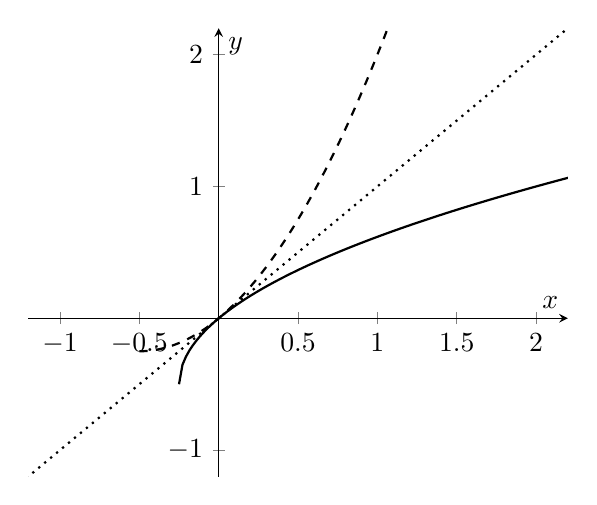
\begin{tikzpicture}
\begin{axis}[axis lines=middle, xlabel=$x$,ylabel=$y$,xmin=-1.2,xmax=2.2,ymin=-1.2,ymax=2.2, samples=150]

\addplot[thick, dashed, color=black,domain=-0.5:3] {x^2+x};
\addplot[thick, color=black,domain=-0.25:3] {(-1+sqrt(1+4*x))/2};
\addplot[thick, dotted, color=black,domain=-2:3] {x};
\end{axis}
\end{tikzpicture}
\end{center}
\caption{\label{gr5} Graf funkcije iz zadatka \ref{invgraph}}
\end{figure}
\end{proof}
\section{Rastav na parcijalne razlomke}

\begin{definition}
\textbf{Racionalna funkcija} je funkcija oblika
$$x\mapsto \dfrac{f(x)}{g(x)},$$
gdje su $f$ i $g$ polinomi i $g\neq 0$ za bar jedan $x\in \mathbb{R}$. Ako je $\st{f}<\st{g}$, onda kažemo da je ona \textbf{prava} racionalna funkcija, a ako je $\st{f}\geq \st{g}$, kažemo da je ona \textbf{neprava}.
\end{definition}

\begin{remark}[O rastavu prave racionalne funkcije na parcijalne razlomke]
\label{partfrac}
Neka su $f$ i $g\neq 0$ polinomi. Svaka prava racionalna funkcija $x\mapsto R(x)=\dfrac{f(x)}{g(x)}$ može se na jedinstven način prikazati kao zbroj parcijalnih razlomaka. Preciznije, zapišimo $g(x)$ u obliku
$$g(x)=(x-x_1)^{k_1}\dots (x-x_s)^{k_s}(x^2+a_1x+b_1)^{l_1}\dots (x^2+a_rx+b_r)^{l_r}.$$
Tada postoje jedinstveni realni brojevi $A_1, \dots, A_{k_1}, D_1,$ $\dots, D_{k_s}, M_1, N_1,$ $ \dots, M_{l_1},$ $ N_{l_1},$ $ \dots R_1,$ $ S_1,$ $\dots, R_{l_r}, S_{l_r}\in \mathbb{R}$ takvi da za sve $x$ iz domene funkcije $x\mapsto R(x)$ vrijedi
\begin{align*}
R(x)&=\dfrac{A_1}{x-x_1}+\dots+\dfrac{A_{k_1}}{(x-x_1)^{k_1}}+\dots+\dfrac{D_1}{x-x_s}+\dots+\dfrac{D_{k_s}}{(x-x_s)^{k_s}} \\
&+\dfrac{M_1x+N_1}{x^2+a_1x+b_1}+\dots+\dfrac{M_{l_1}x+N_{l_1}}{(x^2+a_1x+b_1)^{l_1}}+\dots \\
&+\dfrac{R_1x+S_1}{x^2+a_rx+b_r}+\dots+\dfrac{R_{l_r}x+S_{l_r}}{(x^2+a_rx+b_r)^{l_r}}.
\end{align*}
\end{remark}
Pri rješavanju zadataka trebat će nam još i sljedeći rezultat.
\begin{remark}
\label{poleq}
Neka je $S$ podskup od $\mathbb{R}$ koji se sastoji od svih realnih brojeva, osim možda njih konačno mnogo. Zadane su funkcije $f, g : S\to \mathbb{R}$,
$$f(x)=\sum_{k=0}^n{a_kx^k},\;\;\;g(x)=\sum_{k=0}^m{b_lx^l},$$
gdje su $a_n, b_m\neq 0$. Tada vrijedi $f=g$ ako i samo ako je $m=n$ i $a_j=b_j$ za sve $j=0, 1, \dots, n$.
\end{remark}
Prethodna tvrdnja je zapravo generalizacija teorema o jednakosti polinoma i na one polinome koji nisu definirani na cijelom $\mathbb{R}$.\footnote{U strogom smislu, takve funkcije nisu polinomi, jer ste na predavanju sve polinome definirali na cijelom $\mathbb{R}$, v. \cite{3}.} Međutim, dokaz je potpuno analogan.\footnote{v. \cite{12}, str. 58, 59. Za vježbu pokušajte uočiti što bi trebalo promijeniti u dokazu teorema 1 i 2.}
\begin{exercise}
Rastavite funkciju $x\mapsto \dfrac{1}{(x+2)(x+3)^2}$ na parcijalne razlomke.
\end{exercise}
\begin{proof}[Rješenje]
Prema napomeni \ref{partfrac} znamo da postoje i jedinstveni su brojevi $A$, $B$ i $C$ takvi da za sve $x\in \mathbb{R}\setminus\{-2, -3\}$ vrijedi
$$\dfrac{1}{(x+2)(x+3)^2}=\dfrac{A}{x+2}+\dfrac{B}{x+3}+\dfrac{C}{(x+3)^2}.$$
Želimo odrediti $A$, $B$ i $C$. Pomnožimo li obje strane s $(x+2)(x+3)^2$, proširivanjem dobivamo da za sve $x\in \mathbb{R}\setminus\{-2, -3\}$ vrijedi
$$1=Ax^2+6Ax+9A+Bx^2+5Bx+6B+Cx+2C,$$
odnosno
$$1=(A+B)x^2+(6A+5B+C)x+(9A+6B+2C).$$
Iz prethodnog imamo da su $$P_1, P_2 : \mathbb{R}\setminus\{-2, -3\}\to \mathbb{R},\;P_1(x)=1,\; P_2(x)= (A+B)x^2+(6A+5B+C)x+(9A+6B+2C)$$ jednaki, pa iz napomene \ref{poleq} slijedi
$$\begin{cases}
A+B=0, \\
6A+5B+C=0, \\
9A+6B+2C=1.
   \end{cases}$$
Rješavanjem prethodnog sustava dobivamo $A=1$, $B=-1$ i $C=-1$, pa zaključujemo da je
$$\dfrac{1}{(x+2)(x+3)^2}=\dfrac{1}{x+2}-\dfrac{1}{x+3}-\dfrac{1}{(x+3)^2}.$$
\end{proof}
\begin{exercise}
Dokažite da je funkcija zadana formulom $x\mapsto R(x)=\dfrac{x^3+6x^2+9x+1}{x^2+5x+6}$ injekcija na $\langle -2, \infty\rangle$.
\end{exercise}
\begin{proof}[Rješenje]
Ideja je $R(x)$ prikazati kao sumu jednostavnijih razlomaka, u nadi da ćemo funkciju iz zadatka moći prikazati kao zbroj strogo rastućih funkcija. Dijeljenjem polinoma imamo
$$\dfrac{x^3+6x^2+9x+1}{x^2+5x+6}=x+1+\dfrac{-2x-5}{x^2+5x+6}.$$
Rastavimo $x\mapsto \dfrac{-2x-5}{x^2+5x+6}$ na parcijalne razlomke. Faktorizacijom nazivnika dobivamo $x^2+5x+6=(x+3)(x+2)$. Slijedi da postoje jedinstveni $A$, $B\in \mathbb{R}$ takvi da za sve $x\in \mathbb{R}\setminus\{-2, -3\}$ vrijedi
$$\dfrac{-2x-5}{(x+2)(x+3)}=\dfrac{A}{x+2}+\dfrac{B}{x+3},$$
te množenjem s $(x+2)(x+3)$ dobivamo 
\begin{gather}
\label{partfrac2}
-2x-5=A(x+3)+B(x+2),\;\;\; \forall x\in \mathbb{R}\setminus\{2, 3\}.
\end{gather}
Analogno kao u prethodnom zadatku dobivamo $A, B=-1$. To znači da vrijedi
$$\dfrac{x^3+6x^2+9x+1}{x^2+5x+6}=x+1-\dfrac{1}{x+2}-\dfrac{1}{x+3}$$
za sve $x\in \mathbb{R}\setminus\{-2, -3\}$, pa specijalno i za sve $x\in\langle -2,\infty \rangle$. Kako su $x\mapsto x+1$, $x\mapsto -\dfrac{1}{x+2}$, $x\mapsto -\dfrac{1}{x+3}$ strogo rastuće na $\langle -2,\infty \rangle$, slijedi i da je početna funkcija strogo rastuća na tom intervalu.
\end{proof}
\begin{remark}
Na ovome mjestu bi bilo dobro spomenuti jedan trik koji bi u situacijama poput ove mogao uštedjeti vrijeme. Naime, da bi odredili $A$ i $B$ dovoljno je u (\ref{partfrac2}) uvrstiti $x=-2$ i $x=-3$, respektivno. Međutim, nije odmah očigledno da to možemo, jer u (\ref{partfrac2}) nemamo jednakost polinoma i u točkama $x=2$, $x=3$. 

Tvrdimo da su polinomi jednaki i u tim točkama. Zaista, znamo da svaki polinom koji nije konstanta ima najviše $n$ nultočaka, gdje je $n\in \mathbb{N}$ stupanj polinoma. Kontrapozicijom dobivamo da ako proizvoljan polinom ima beskonačno mnogo nultočaka, onda je on nužno konstanta. No lako vidimo da je jedini polinom koji uopće ima nultočku nul-polinom. 

Posljedica prethodne tvrdnje je sljedeća -- ako su dva polinoma jednaka u beskonačno mnogo točaka, onda su oni jednaki za sve realne brojeve. Zaista, neka su $f$ i $g$ polinomi koji su jednaki u beskonačno mnogo točaka. No tada $f-g$ ima beskonačno mnogo nultočaka, a to znači da je $f-g=0$, odnosno $f=g$. Time smo dokazali tvrdnju. 

Kako su u našem slučaju polinomi $x\mapsto -2x-5$ i $x\mapsto A(x+3)+B(x+2)$ očito jednaki u beskonačno mnogo točaka, oni su sigurno jednaki i u $x=-2$ i $x=-3$, što smo i tvrdili.
\end{remark}
\section{Prirodna domena}
\begin{remark}
Neka je $x\mapsto f(x)$ funkcija zadana formulom. Skup svih $x\in \mathbb{R}$ za koju je $f(x)$ dobro definiran zove se \textbf{prirodna domena} funkcije $f$.
\end{remark}

\begin{exercise}
Odredite prirodnu domenu funkcije $x\mapsto f(x)$, ako je
\begin{itemize}
\item[a)] $f(x)=\sqrt{\log_2(x^2-1)}$,
\item[b)] $f(x)=\arcosh(x^2-4x)+\cth(x-6)$,
\item[c)] $f(x)=\artanh{\sqrt{x}}+\log_2(x+2)$.
\end{itemize}
\end{exercise}
\begin{proof}[Rješenje]
a) Uočimo da je domena od $x\mapsto \log_2{x}$ jednaka $\mathbb{R}^+$, a domena od $x\mapsto \sqrt{x}$ jednaka $[0, \infty\rangle$. Zato trebaju biti zadovoljeni sljedeći uvjeti:
\begin{itemize}
\item $x^2-1>0$,
\item $\log_2(x^2-1)\geq 0$.
\end{itemize}
Prvi uvjet vrijedi ako i samo ako je $x\in \langle-\infty, -1\rangle\cup \langle 1, \infty\rangle$.

Promotrimo drugi uvjet. Uočimo da vrijedi $$\log_2(x^2-1)\geq 0\Leftrightarrow x^2-1\geq 1,$$
za sve $x\in \langle-\infty, -1\rangle\cup \langle 1, \infty\rangle$ (Uvjerite se u to!). No ovo je ekvivalentno tvrdnji $x\in \langle-\infty, -\sqrt{2}\rangle\cup \langle \sqrt{2}, \infty\rangle$. Dakle, domena funkcije $f$ je upravo $$\langle-\infty, -\sqrt{2}\rangle\cup \langle \sqrt{2}, \infty\rangle.$$

b) Uočimo da je domena od $x\mapsto \arcosh{x}$ jednaka $[1, \infty\rangle$, a domena od $x\mapsto \cth{x}$ je jednaka $\mathbb{R}\setminus\{0\}$. Imamo sljedeće uvjete:
\begin{itemize}
\item $x^2-4x\geq 1$,
\item $x-6\neq 0,\text{ odnosno } x\neq 6$.
\end{itemize}
Rješenje nejednadžbe $x^2-4x\geq 1$ je $x\in \langle -\infty, 2-\sqrt{5}]\cup [2+\sqrt{5}, \infty\rangle$, pa je domena
$$\langle -\infty, 2-\sqrt{5}]\cup [2+\sqrt{5}, \infty\rangle\setminus\{6\}.$$

c) Uočimo da je domena od $x\mapsto \artanh{x}$ jednaka $\langle -1, 1\rangle$. Odavde slijedi da trebaju biti zadovoljeni sljedeći uvjeti:
\begin{itemize}
\item $x\geq 0$,
\item $x+2>0,\text{ odnosno }x>-2$,
\item $\sqrt{x}\in \langle -1, 1\rangle$.
\end{itemize}
Primijetimo da drugi uvjet možemo zanemariti. Nadalje, treba vrijediti $\sqrt{x}>-1$ i $\sqrt{x}<1$. $\sqrt{x}>-1$ je istinita za sve realne $x$, pa je možemo zanemariti. Nadalje, vrijedi $\sqrt{x}<1$ ako i samo ako vrijedi $ x<1$. Dakle, domena početne funkcije je $[0, 1\rangle$.
\end{proof}
\begin{exercise}
Odredite sve $x\in \mathbb{R}$ za koje vrijedi
$$\arcsin{\dfrac{\log_2(x+2)}{2}}=\sqrt{-x-\dfrac{7}{4}}-\dfrac{\pi}{2}.$$
\end{exercise}
\begin{proof}[Rješenje]
Prvo bi bilo dobro vidjeti kad su oba izraza definirana. Drugim riječima, trebamo odrediti prirodne domene funkcija $x\mapsto \arcsin{\dfrac{\log_2(x+2)}{2}}$ i $x\mapsto \sqrt{-x-\dfrac{7}{4}}-\dfrac{\pi}{2}$. Lako se vidi da je domena funkcije $x\mapsto \sqrt{-x-\dfrac{7}{4}}-\dfrac{\pi}{2}$ jednaka $\left\langle -\infty, -\dfrac{7}{4}\right]$.

Odredimo domenu funkcije $x\mapsto \arcsin{\dfrac{\log_2(x+2)}{2}}$. Sjetimo se da je domena funkcije $x\mapsto \arcsin{x}$ jednaka $[-1, 1]$. Zato trebaju biti zadovoljeni sljedeći uvjeti:
\begin{itemize}
\item $x+2>0$, odnosno $x>-2$,
\item $\dfrac{\log_2(x+2)}{2}\in [-1, 1]$.
\end{itemize}
Očito za sve $x>-2$ vrijedi $\dfrac{\log_2(x+2)}{2}\in [-1, 1]$ ako i samo ako je
$$-2\leq \log_2(x+2)\leq 2,$$
što je ekvivalentno tvrdnji
$$\dfrac{1}{4}\leq x+2\leq 4,$$
što vrijedi ako i samo ako je $x\in \left[-\dfrac{7}{4}, 2\right]$. Dakle jedini realan broj za kojeg su oba izraza definirana je upravo $\dfrac{7}{4}$. No lako se provjeri da $x\mapsto \arcsin{\dfrac{\log_2(x+2)}{2}}$ i $x\mapsto \sqrt{-x-\dfrac{7}{4}}-\dfrac{\pi}{2}$ poprimaju vrijednost $-\dfrac{\pi}{2}$ za $x=\dfrac{7}{4}$. Zato je to jedino rješenje početne jednadžbe.
\end{proof}
\begin{exercise}
Neka je $x\mapsto f(x)$ funkcija zadana formulom $f(x)=\arccos\left(\tg\left(1+\dfrac{1}{x}\right)\right)$. Odredite prirodnu domenu ove funkcije.
\end{exercise}
\begin{proof}[Rješenje]
Trebaju biti zadovoljeni sljedeći uvjeti:
\begin{itemize}
\item $x\neq 0$,
\item $1+\dfrac{1}{x}\notin \left\{\dfrac{\pi}{2}+k\pi : k\in \mathbb{Z}\right\}$,
\item $\tg\left(1+\dfrac{1}{x}\right)\in [-1, 1]$.
\end{itemize}
Vrijedi $\tg\left(1+\dfrac{1}{x}\right)\in [-1, 1]$ ako i samo ako je
\begin{gather}
\label{4}
1+\dfrac{1}{x}\in \bigcup_{k\in \mathbb{Z}}{\left[-\dfrac{\pi}{4}+k\pi, \dfrac{\pi}{4}+k\pi\right]},
\end{gather}
odnosno ako i samo ako (v. napomenu \ref{unprfam}) postoji $k\in \mathbb{Z}$ takav da je
$$-\dfrac{\pi}{4}+k\pi\leq 1+\dfrac{1}{x} \leq \dfrac{\pi}{4}+k\pi.$$
Primijetimo da (\ref{4}) obuhvaća i činjenicu $1+\dfrac{1}{x}\notin \left\{\dfrac{\pi}{2}+k\pi : k\in \mathbb{Z}\right\}$. Uočimo da je (\ref{4}) ekvivalentno uvjetu
\begin{gather}
\label{5}
-\dfrac{\pi}{4}-1+k\pi\leq \dfrac{1}{x} \leq \dfrac{\pi}{4}-1+k\pi.
\end{gather}
Htjeli bismo odavde dobiti u kojem segmentu se nalazi $x$. Uočimo prvo da su svi intervali $\left[-\dfrac{\pi}{4}-1+k\pi, \dfrac{\pi}{4}-1+k\pi\right]$ podskupovi jednog (i samo jednog) od skupova $\langle -\infty, 0\rangle$ i $\langle 0, \infty\rangle$. Zaista, za $k\geq 1$ vrijedi
$$-\dfrac{\pi}{4}-1+k\pi\geq -\dfrac{\pi}{4}-1+\pi>0$$
i analogno $\dfrac{\pi}{4}-1+k\pi<0$ za $k\leq 0$. Dakle, za $k\geq 1$ imamo $\dfrac{1}{x}>0$, odnosno $x>0$, pa možemo "množiti" s $x$ i $\dfrac{\pi}{4}-1+k\pi$. U tom slučaju dobivamo
$$x\in \bigcup_{k\in \mathbb{Z}}{\left[\dfrac{1}{\dfrac{\pi}{4}-1+k\pi}, \dfrac{1}{-\dfrac{\pi}{4}-1+k\pi}\right]},$$
Analogno, ako je $k\leq 0$, onda također možemo "množiti" s  $x$ i $\dfrac{\pi}{4}-1+k\pi$, ali se pritom mijenja predznak. Analogno dobivamo
$$x\in \bigcup_{k\in \mathbb{Z}\setminus{\mathbb{N}}}{\left[\dfrac{1}{\dfrac{\pi}{4}-1+k\pi}, \dfrac{1}{-\dfrac{\pi}{4}-1+k\pi}\right]},$$
te kako oba uvjeta obuhvaćaju i uvjet $x\neq 0$ (jer su ili oba "ruba" segmenta negativna ili oba pozitivna), slijedi da je prirodna domena početne funkcije upravo 
\begin{align*}
\bigcup_{k\in \mathbb{N}}{\left[\dfrac{1}{\dfrac{\pi}{4}-1+k\pi}, \dfrac{1}{-\dfrac{\pi}{4}-1+k\pi}\right]}&\cup \bigcup_{k\in \mathbb{Z}\setminus{\mathbb{N}}}{\left[\dfrac{1}{\dfrac{\pi}{4}-1+k\pi}, \dfrac{1}{-\dfrac{\pi}{4}-1+k\pi}\right]}\\
=\bigcup_{k\in \mathbb{Z}}{\left[\dfrac{1}{\dfrac{\pi}{4}-1+k\pi}, \dfrac{1}{-\dfrac{\pi}{4}-1+k\pi}\right]}.
\end{align*}
\end{proof}
\newpage
\begin{remark}
Uočite da smo u prethodnom zadatku primijenili vrlo intuitivnu činjenicu da je za sve familije $\mathcal{F}=\{A_n : n\in \mathbb{Z}\}$, $\mathcal{F}'=\{A_n : n\in \mathbb{N}\}$ i $\mathcal{F}''=\{A_n : n\in \mathbb{Z}\setminus\mathbb{N}\}$,
$$\bigcup_{k\in \mathbb{Z}}{A_n}=\bigcup_{k\in \mathbb{N}}{A_n}\cup \bigcup_{k\in \mathbb{Z}\setminus\mathbb{N}}{A_n}.$$
Dokažimo to! Zaista, vrijedi $\displaystyle x\in \bigcup_{k\in \mathbb{N}}{A_n}\cup \bigcup_{k\in \mathbb{Z}\setminus\mathbb{N}}{A_n}$ ako i samo ako ili postoji $i\in \mathbb{N}$ takav da je $x\in A_i$, ili postoji $j\in \mathbb{Z}\setminus\mathbb{N}$ takav da je $x\in A_j$. Očito, to vrijedi ako i samo ako postoji $k\in \mathbb{Z}$ takav da je $x\in A_k$, tj. $\displaystyle x\in \bigcup_{k\in \mathbb{Z}}{A_n}$.
\end{remark}

\section{Periodične funkcije}

\begin{definition}
Neka je zadana funkcija $f : A\to B$, $A$, $B\subseteq \mathbb{R}$ i $\tau>0$. Kažemo da je $f$ \textbf{periodična s periodom $\tau$} ako za sve $x\in A$ vrijedi $x+\tau \in A$ i $f(x+\tau)=f(x)$. Najmanji od svih perioda, ako postoji, zvat ćemo \textbf{temeljnim periodom}.
\end{definition}

Lako vidimo iz grafova od $\sin$ i $\cos$ da su oni periodični s temeljnim periodom $2\pi$. Nadalje, funkcija $x\mapsto c$, $c\in \mathbb{R}$ je periodična i ona nema temeljni period.
\begin{exercise}
Dokažite da je $x\mapsto \sin{x}$ periodična s temeljnim periodom $2\pi$.
\end{exercise}
\begin{proof}[Rješenje]
Znamo da $x\mapsto \sin{x}$ ima domenu $\mathbb{R}$, pa je tvrdnja o domeni trivijalno zadovoljena za bilo koji $\tau\in \mathbb{R}$. Znamo i da je $$\sin(x+2\pi)=\sin{x},\;\;\; \forall x\in \mathbb{R}.$$ Još preostaje pokazati da je $2\pi$ temeljni period. 

Pretpostavimo da postoji neki period $\tau_0$ takav da je $\tau_0<2\pi$. Tada je $\sin(x+\tau_0)=\sin{x}$. Specijalno, iz definicije za $x=0$ imamo $\sin{\tau_0}=0$. To je moguće ako i samo ako je $$x\in \{k\pi : k\in \mathbb{Z}\}.$$ No kako imamo $0<\tau_0<2\pi$ slijedi nužno $\tau_0=\pi$. No $\pi$ očito nije period, jer je npr. $\sin{\dfrac{\pi}{2}}=1$ i $\sin\left(\dfrac{\pi}{2}+\pi\right)=-1$.
\end{proof}
\begin{exercise}
Funkcija $D : \mathbb{R}\to \mathbb{R}$,
$$D(x)=\begin{cases}
0, & x\in \mathbb{I},\\
1, & x\in \mathbb{Q}
\end{cases}$$
zove se \textit{Dirichletova funkcija}. Dokažite da je ona periodična, ali nema temeljni period.
\end{exercise}
\begin{proof}[Rješenje]
Tvrdimo da je svaki pozitivan $\tau\in \mathbb{Q^+}$ jedan period funkcije $D$. Odavde će biti očito da je $D$ periodična i da nema temeljni period.

Zaista, neka je $x\in \mathbb{R}$ proizvoljan. Tvrdimo da je $x\in \mathbb{Q}$ ako i samo ako je $x+\tau\in \mathbb{Q}$. Zaista, ako je $x\in \mathbb{Q}$, onda je očito $x+\tau\in \mathbb{Q}$. Nadalje, ako je $x+\tau\in \mathbb{Q}$, iz činjenice da je $-\tau\in \mathbb{Q}$ slijedi da je i $(x+\tau)-\tau=x\in \mathbb{Q}$.

Kontrapozicijom slijedi: Ako je $x\in \mathbb{Q}$, onda je $x+\tau\in \mathbb{Q}$, te ako je $x\in \mathbb{I}$ iracionalan, onda je i $x+\tau\in \mathbb{I}$. U oba slučaja imamo $f(x+\tau)=f(x)$ i tvrdnja je dokazana.
\end{proof}
\begin{exercise}
Je li funkcija $x\mapsto x\sin{x}$ periodična?
\end{exercise}
\begin{proof}[Rješenje]
Iz grafa funkcije možemo naslutiti da ona nije periodična.
\begin{figure}[ht]
\begin{center}
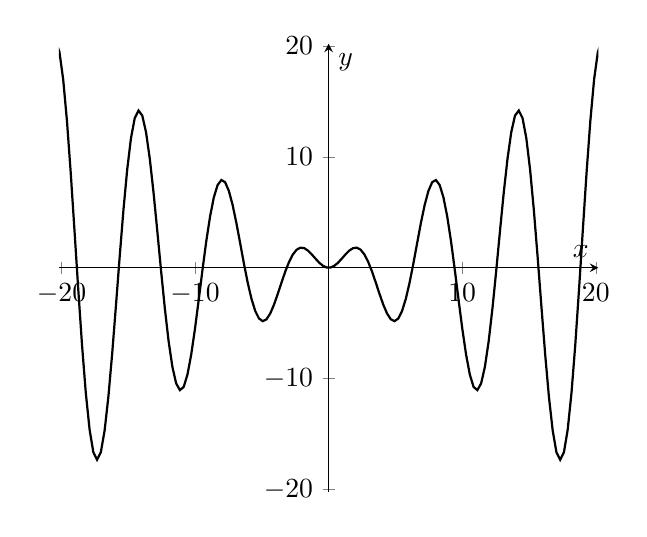
\begin{tikzpicture}
\begin{axis}[axis lines=middle, xlabel=$x$,ylabel=$y$,xmin=-20.2,xmax=20.2,ymin=-20.2,ymax=20.2, samples=150]

\addplot[thick, color=black,domain=-21:21] {x*sin(deg(x))};
\end{axis}
\end{tikzpicture}
\end{center}
\caption{\label{gr6} Graf funkcije $x\mapsto x\sin{x}$}
\end{figure}

Dokažimo tvrdnju. Zaista, pretpostavimo da postoji neki period $\tau>0$. Funkcija je definirana za sve realne brojeve, pa je $x+\tau\in \mathcal{D}(f)$. Po pretpostavci imamo $$(x+\tau)\sin(x+\tau)=x\sin{x},\; \forall x\in \mathbb{R}.$$ 
Specijalno, za $x=-\tau$ imamo $\tau\sin{\tau}=0$, odnosno $\sin{\tau}=0$. To je ekvivalentno sa $\tau\in \{k\pi : k\in \mathbb{N}\}$, gdje je $k\in \mathbb{N}$ jer je $\tau>0$, po definiciji perioda. No to znači da postoji $k\in \mathbb{N}$ takav da je $$(x+k\pi)\sin(x+k\pi)=x\sin{x},\;\forall x\in \mathbb{R}.$$ Ako je $k$ paran, onda je $\sin(x+k\pi)=\sin{x}$. Uzmimo $x$ takav da je $\sin{x}\neq 0$. Tada dijeljenjem sa $\sin{x}$ dobivamo $\pi=0$, kontradikcija! 

Ako je $k$ neparan, onda je $\sin(x+k\pi)=-\sin{x}$. Uzmimo $x$ takav da je $x\in \mathbb{N}$. Zaista, kako je $\pi\in \mathbb{I}$, vrijedi $\sin{x}\neq 0$, jer bi u suprotnom imali $\dfrac{x}{k}=\pi$. Dijeljenjem sa $\sin{x}$ dobivamo $-x-k\pi=x$, odnosno $-\dfrac{2x}{k}=\pi$. Kontradikcija s činjenicom da je $\pi\in \mathbb{I}$! Dakle slijedi $\tau\notin \{k\pi : k\in \mathbb{N}\}$, čime imamo kontradikciju s činjenicom $\tau\in \{k\pi : k\in \mathbb{N}\}$, i time smo dokazali tvrdnju.
\end{proof}
\newpage
\section*{Zadatci za vježbu}
\addtocontents{toc}{\protect\pagebreak[4]}
\subsection*{Pojam funkcije. Crtanje grafa funkcije}
\begin{exercise}
Nacrtajte grafove sljedećih funkcija. (Kada je interval cijeli $\mathbb{R}$, prikažite "najreprezentativniji" dio grafa). 
\begin{itemize}
\item[a)] $f : [-1, 1]\to \mathbb{R}$, $f(x)=x^2+4x+5$,
\item[b)] $f : \mathbb{R}\to \mathbb{R}$, $f(x)=|x+2|-|x|$,
\item[c)] $f : \mathbb{R}\to \mathbb{R}$, $f(x)=(x-2025)^3-2025$.
\item[d)] $f : \mathbb{R}\setminus\{0\}\to \mathbb{R}$, $f(x)=x+\dfrac{1}{x}$.
\end{itemize}
\end{exercise}
\begin{exercise} Promotrite sljedeću sliku.
\begin{figure}[ht]
\begin{center}
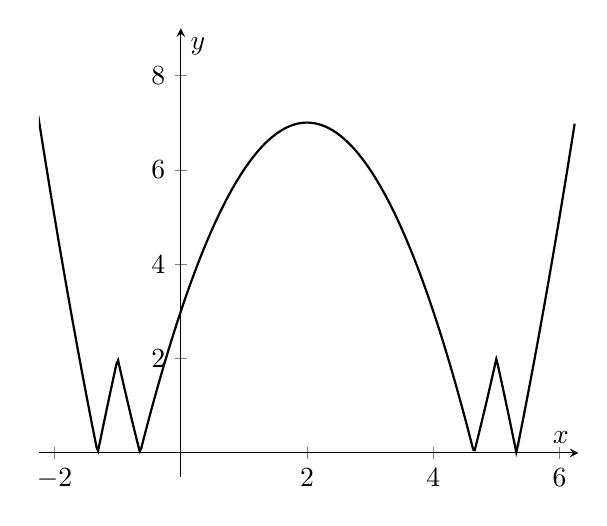
\begin{tikzpicture}
\begin{axis}[axis lines=middle, xlabel=$x$,ylabel=$y$,xmin=-2.25,xmax=6.3,ymin=-0.5,ymax=9, samples=350]

\addplot[thick, color=black,domain=-2.26:6.24] {abs(abs(x*x-4*x-5)-2)};
\end{axis}
\end{tikzpicture}
\end{center}
\end{figure}

Ako je poznato da postoje $a, b, c\in \mathbb{R}$, $a\neq 0$ takvi da je graf na slici upravo graf funkcije $f(x)=\left|\left|ax^2+bx+c\right|-2\right|$, odredite neke takve $a, b, c$.
\end{exercise}
\subsection*{Injekcija, surjekcija i bijekcija. Slika i praslika skupa}
\begin{exercise}
Za svaku od sljedećih funkcija odredite je li bijekcija. Ako smatrate da je, dokažite da je, u suprotnom dokažite zašto nije.
\begin{itemize}
\item[a)] $f : \mathbb{R}\to \mathbb{R}$, $f(x)=x^4-x^2$,
\item[b)] $f : \mathbb{R}\to \mathbb{R}$, $f(x)=2x^3+3$.
\item[c)] $f : \mathbb{R}\to [-2, \infty]$, $f(x)=e^x-2$,
\end{itemize}
\end{exercise}
\begin{exercise} \textbf{}
\begin{itemize}
\item[a)] Navedite primjer rastuće funkcije $f : \mathbb{R}\to [-1, 1]$.
\item[b)] Navedite primjer padajuće funkcije s $\mathbb{R}$ u $\mathbb{R}$ koja nije ni injekcija ni surjekcija.
\item[b)] Navedite primjer bijekcije $f : \mathbb{R}\to \langle 10, \infty\rangle$.
\item[c)] Navedite primjer bijekcije $f : \langle 10, 20\rangle\to \mathbb{R}$.
\item[d)] Navedite primjer surjekcije $f : \mathbb{R}\to [-1, 0\rangle\cup \langle 0, 1]\cup \{2025\}$.
\item[e)] Navedite primjer surjekcije $f : \mathbb{R}\to \langle -1, 1\rangle \cup \mathbb{N}$.
\end{itemize}
\end{exercise}
\begin{exercise} \textbf{}
\begin{itemize}
\item[a)] Navedite primjer funkcije $f : \mathbb{R}\to \mathbb{R}$ za koju vrijedi $f([0, 5])=[2, 3]$.
\item[b)] Navedite primjer funkcije $f : \mathbb{R}\to \mathbb{R}$ za koju vrijedi $f([0, 5])=[2, 3]$ \textbf{i} $f^{-1}\left(\langle 5, 15]\right)=[-2, -1\rangle \cup \langle 5, 7.5]$.
\item[c)] Postoji li funkcija $f : \mathbb{R}\to \mathbb{R}$ za koju vrijedi $f\left([0, 1]\right)=[1, 2]$ i $f^{-1}\left([1, 3]\right)=[4, 5]$? Dokažite svoje tvrdnje.
\item[d)] Neka je zadana $f : S\to \mathbb{R}$ i neka su $A$, $B\subseteq S$. Dokažite da je $f(A\cap B)=f(A)\cap f(B)$ ako i samo ako je $f$ injekcija.
\end{itemize}
\end{exercise}
\begin{exercise} $(*)$ Neka je $g : \mathbb{R}\to \mathbb{R}$ funkcija takva da je za svaku injekciju $f : \mathbb{R}\to \mathbb{R}$, funkcija $f+g$ također injekcija. Dokažite da je tada $g$ konstanta.
\end{exercise}
\subsection*{Kompozicija funkcija. Inverzna funkcija}
\begin{exercise}
Neka su zadane $f : A\to B$ i $g : B\to C$. Dokažite da ako je $g\circ f$ injekcija, onda je i $f$ injekcija.
\end{exercise}
\begin{exercise}
Neka je $f : \mathbb{R} \to \mathbb{R}$ zadana formulom $f(x)=x^3-2x^2$.
\begin{itemize}
\item[a)] Nacrtajte graf funkcije $f$.
\item[b)] Dokažite da je $f|_{[0, 1]}$ injekcija. Je li $f$ injekcija?
\item[c)] Odredite $f^{-1}\left([0, 9]\right)$ i $f^{-1}\left([2024, 2025]\right)\cap f^{-1}\left([23, 24]\right)$.
\item[d)] Koristeći graf, odredite $f\left([2, 2.2\rangle\right)$.
\end{itemize}
\end{exercise}
\begin{exercise} \textbf{}
\begin{itemize}
\item[a)] Zadana je $f : \mathbb{R}\to \mathbb{R}$, $f(x)=x^4+3|x|^3+4$. Odredite $\mathcal{R}(f)$.
\item[b)] Zadana je $f : [0, \infty\rangle\to \mathbb{R}$, $f(x)=e^{\frac{1-\sqrt{x}}{1+\sqrt{x}}}$. Odredite $f^{-1}\left([1, e]\right)$.
\item[d)] Odredite primjer funkcije $f : \mathbb{R}\to \mathbb{R}$ za koju je $f^{-1}\left([4, 5]\right)=[-3, 2]\cup [6, 7]$.
\end{itemize}
\end{exercise}
\begin{exercise} \textbf{}
\begin{itemize}
\item[a)] Dokažite da je $f : \left[0, \dfrac{\pi}{2}\right]\to [4, 8]$ za koju je $f(x)=\sin^4{x}+3\sin^2{x}+4$ bijekcija i odredite njezin inverz.
\item[a)] Odredite skup $S$ (ako postoji) takav da $f : \mathbb{R}\to S$, $f(x)=\th^3{x}+1$ bude bijekcija.
\item[b)] Neka je $f : \mathbb{R}\to [-2, \infty\rangle$ zadana formulom $f(x)=\abs{\abs{\abs{x}-2}-2}-2$. 
Ispitajte injektivnost, surjektivnost i koristeći graf odredite $f^{-1}\left(\left[\dfrac{1}{2}, 4\right\rangle\right)$.
\end{itemize}
\end{exercise}
\begin{exercise} \textbf{}
\begin{itemize}
\item[a)] Odredite neki $a\in\mathbb{R}$ (ako postoji) takav da je $f : [a, \infty\rangle\to \mathbb{R}$, $f(x)=x^4-2x^2$ injekcija.
\item[b)] Neka su zadane $f, g : S\to \mathbb{R}$. Dokažite ili opovrgnite: Ako su $f$ i $g$ strogo rastuće i ako vrijedi $f(x)\geq 0$ i $g(x)\geq 0$ za sve $x\in S$, onda je i $fg$ strogo rastuća.
\item[c)] Odredite sve $x\in \mathbb{R}$ takve da je $x^3-2x=4$. (Dokažite svoje tvrdnje!)
\end{itemize}
\end{exercise}
\begin{exercise} $(*)$
Neka je $f : \mathbb{R}\to \mathbb{R}$ dana izrazom $f(x)=\dfrac{x}{\sqrt{1+x^2}}$. Neka je $f_n(x)=\underbrace{f(f(\dots f(x))\dots)}_\text{$n$ puta}$. Izračunajte $f_{2024}(2024)$ i pokažite da je $f_{2024}$ injekcija.
\end{exercise}
\begin{exercise} $(*)$
Zadana je $f : \mathbb{R}\to \mathbb{R}$,
$$f(x)=(x+2)(x+3)(x+7)(x+8)$$
Odredite $\mathcal{R}(f)$.
\end{exercise}
\begin{exercise} $(*)$ Izračunajte
$$\arctg{\dfrac{1}{2}}+\arctg{\dfrac{1}{8}}+\arctg{\dfrac{1}{18}}+\dots+ \arctg{\dfrac{1}{2\cdot 2024^2}}.$$
\end{exercise}
\begin{exercise} $(**)$
Može li se funkcija $x\mapsto x\cos(x^3-x)$ prikazati kao kompozicija konačno mnogo funkcija $x\mapsto -x$, $x\mapsto x\sin{x}$, $x\mapsto \sh{x}$, $x\mapsto x^3+x$? Dokažite.
\end{exercise}
\subsection*{Rastav na parcijalne razlomke}
\begin{exercise}
Rastavite sljedeće funkcije na parcijalne razlomke (po potrebi prvo funkciju prikazati kao zbroj polinoma i prave racionalne funkcije). 
\begin{itemize}
\item[a)] $x\mapsto \dfrac{x^3+2x+3}{x^3-x}$,
\item[b)] $x\mapsto \dfrac{1}{x^3+1}$.
\end{itemize}
\end{exercise}
\begin{exercise}
Zadana je $f : \mathbb{R}\setminus\{-1\}\to\mathbb{R}$,
$$f(x)=\dfrac{x^3+6x^2+12x+9}{(x+1)^3}.$$
Odredite $f\left([0, 2]\right)$.
\end{exercise}
\begin{exercise} $(*)$ \textbf{}
Zadan je sustav jednadžbi
$$\begin{cases}
A + C&=9,\\
 3A + B + C + D&=5,\\
 2A + 4B - 2C + E&=7,\\
 -2A + 6B - 2C - 2D - E + F&=4,\\
 -3A + 4B + C - E - 2F&=6,\\
 -A + B + C + D + E + F&=3
   \end{cases}$$
Dokažite (bez korištenja rezultata iz linearne algebre i bez rješavanja sustava) da ovaj sustav ima jedinstveno rješenje, tj. da postoje jedinstveni $A, B, C, D, E, F\in \mathbb{R}$ za koje vrijedi sustav jednadžbi.
\end{exercise}
\subsection*{Prirodna domena}
\begin{exercise}
Odredite prirodnu domenu sljedećih funkcija.
\begin{AutoMultiColItemize}
\item[a)] $x\mapsto \mathrm{arch}\left(\arccos{\dfrac{x-1}{x+2}}+1\right)$,
\item[b)] $x\mapsto \dfrac{1}{\sqrt{1-\dfrac{1}{x}}}$
\item[c)] $x\mapsto \arcsin{\sin{x}}$,
\item[d)] $x\mapsto \sqrt{1+\log\lfloor x^2-1\rfloor},$
\item[e)] $x\mapsto \ln\left(\dfrac{1}{\sin{x}}-2\cos{x}\right).$
\end{AutoMultiColItemize}
\end{exercise}
\begin{exercise} Navedite primjer elementarne funkcije čija je prirodna domena:
\begin{itemize}
\item[a)] $[1, \infty\rangle \setminus \{2\}$,
\item[b)] $\langle 1, \infty\rangle \setminus{\mathbb{N}}$.
\item[c)] $\langle -\infty, 2]\cup [3, \infty\rangle$.
\end{itemize}
(\textbf{Uputa:} Elementarne funkcije su sve one funkcije koje se mogu dobiti pomoću konačnog broja operacija zbrajanja, množenja, oduzimanja, dijeljenja i kompozicije iz potencija, eksponencijalnih, hiperbolnih, trigonometrijskih funkcija i njihovih inverznih funkcija -- korijena, logaritamskih, area i arkus funkcija).
\end{exercise}
\subsection*{Periodične funkcije}
\begin{exercise}
Je li $x\mapsto \sin^2{x}$ periodična? Ako je, koji joj je temeljni period?
\end{exercise}

\chapter{Nizovi}
\fancyhead[RO, RE]{}
\fancyhead[LO, LE]{\large Nizovi}

\section{Pojam niza. Limes niza}
\begin{definition} \textbf{}
\begin{itemize}
\item Funkcija $a : \mathbb{N}\to S$ zove se \textbf{niz} na $S$. Specijalno, ako je $S=\mathbb{R}$, radi se o nizu realnih brojeva, ako je $S=\mathbb{C}$ radi se o nizu kompleksnih brojeva, a ako je $S$ skup svih funkcija definiranih na nekom skupu, kažemo da imamo niz funkcija.

\item Kažemo da je $a(n)$ $n$-ti član niza, u oznaci $a_n$. Općenito, alternativna oznaka za niz $a$ koju ćemo često koristiti je $(a_n)$. 

\item Na nekim mjestima, ako je jasno kako se niz nastavlja, možemo niz zadati "nizanjem" njegovih prvih nekoliko elemenata:
$$a_1,\; a_2,\; a_3,\;\dots, a_n,\; \dots $$
\end{itemize}
\end{definition}
U daljnjem tekstu, ako nije navedeno drukčije, smatrat ćemo da se radi o nizu realnih brojeva.
\begin{definition}
\textbf{Aritmetički niz} s prvim članom $a_1$ i razlikom $d$ je niz $(a_n)$ zadan općim članom
$$a_n=a_1+(n-1)d, \; n\in \mathbb{N}.$$
\end{definition}

\noindent Iz definicije aritmetičkog niza slijedi:
\begin{itemize}
\item $a_{n+1}-a_n=d$,
\item $\dfrac{a_{n-1}+a_{n+1}}{2}=a_n, \; n\geq 2,$
\item Neka je $S_n=a_1+a_2+\dots+a_n$. Vrijedi
\begin{gather}
\label{arsum}
S_n=\dfrac{n}{2}\left(a_1+a_n\right), \; S_n=\dfrac{n}{2}\left(2a_1+(n-1)d\right)
\end{gather}
\end{itemize}
\begin{definition}
\label{17}
\textbf{Geometrijski niz} s prvim članom $a_1$ i kvocijentom $q\neq 0$ je niz $(a_n)$ zadan općim članom
$$a_n=a_1\cdot q^{n-1}, \; n\in \mathbb{N}.$$
\end{definition}

\noindent Iz definicije geometrijskog niza slijedi:
\begin{itemize}
\item $\dfrac{a_{n+1}}{a_n}=q$,
\item $\sqrt{a_{n-1}\cdot a_{n+1}}=a_n, \; n\geq 2,$
\item Neka je $S_n=a_1+a_2+\dots+a_n$. Vrijedi
\begin{gather}
\label{geosum}
S_n=\begin{cases}
na_1, & q=1, \\
a_1\dfrac{1-q^n}{1-q}, & q\neq 1.
   \end{cases}
\end{gather}
\end{itemize}
\begin{exercise}\textbf{}
\begin{itemize}
\item[a)] Neka je $(a_n)$ geometrijski niz, $a_1=64$ i $a_7=15625$. Odredite $a_3$.
\item[b)] Niz $(a_n)$ zadan je općim članom $a_n=-3+\dfrac{1}{4}(n-1)$. Ako je zbroj prvih $m$ članova niza $\dfrac{21}{2}$, koliko je $m$?
\end{itemize}
\end{exercise}
\begin{proof}[Rješenje]
a) Po definiciji, za niz $(a_n)$ vrijedi $a_n=64\cdot q^n$. Nadalje, dobivamo jednadžbu
$$a_7=64\cdot q^6=15625,\text{ čije je rješenje } q=\dfrac{5}{2}.$$
Odavde direktno slijedi $a_3=64\cdot \left(\dfrac{5}{2}\right)^2=400.$

b) Uočimo da je niz $(a_n)$ aritmetički, pa vrijedi (\ref{arsum}). Imamo
$$\dfrac{m}{2}\left(-6+\dfrac{1}{4}(m-1)\right)=\dfrac{21}{2}.$$
Rješavanjem kvadratne jednadžbe dobivamo $m_1=28$ i $m_2=-3$. Kako je $(a_n)$ definiran samo za $n\in \mathbb{N}$, slijedi da je jedino moguće rješenje $m=28$.
\end{proof}
\begin{definition}
Niz $(a_n)$ u $\mathbb{R}$ je \textbf{rastući} ako za sve $n\in \mathbb{N}$ vrijedi $a_n\geq a_{n+1}$, \textbf{strogo rastući} ako za sve $n\in \mathbb{N}$ vrijedi $a_n<a_{n+1}$, \textbf{padajući} ako za sve $n\in \mathbb{N}$ vrijedi $a_n\geq a_{n+1}$, te \textbf{strogo padajući} ako za sve $n\in \mathbb{N}$ vrijedi $a_n>a_{n+1}$.
\end{definition}

\begin{exercise}\textbf{}
\begin{itemize}
\item[a)] Dokažite da je niz $(a_n)$ zadan formulom $a_n=2^n+n$ strogo rastući.
\item[b)] Dokažite da je niz $(a_n)$ zadan formulom $a_n=\sqrt{n+1}-\sqrt{n}$ strogo rastući.
\item[c)] Dokažite da je niz $(a_n)$ zadan formulom $a_n=\dfrac{n^2+1}{n^2-1}$ strogo padajući.
\end{itemize}
\end{exercise}
\begin{proof}[Rješenje]
a) Treba dokazati da za sve $n\in \mathbb{N}$ vrijedi $2^{n+1}+n+1>2^n+n$. Očito vrijedi $$2^{n+1}+n+1>2^{n+1}+n>2^n+n, \;\;\forall n\in \mathbb{N},$$
pa je tvrdnja dokazana.

b) Treba dokazati da za sve $n\in \mathbb{N}$ vrijedi $\sqrt{n+2}-\sqrt{n+1}>\sqrt{n+1}-\sqrt{n}$. Znamo da je $$-\sqrt{n}>-\sqrt{n+1}\;\text{ i }\;\sqrt{n+2}>\sqrt{n+1}\;\;\forall n\in \mathbb{N}.$$ Zbrajanjem tih dvaju jednakosti dobivamo tvrdnju.

c) Neka je $n\in \mathbb{N}$ proizvoljan. Vrijedi $\dfrac{n^2+1}{n^2-1}=1+\dfrac{2}{n^2-1}$. Sada treba pokazati da za sve $n\in \mathbb{N}$ vrijedi 
$$1+\dfrac{2}{n^2-1}>1+\dfrac{2}{(n+1)^2-1}.$$
No to je ekvivalentno s tvrdnjom $(n+1)^2>n^2$, što je očigledno istinito za sve $n\in \mathbb{N}$.
\end{proof}

\begin{definition}
Niz $(a_n)$ je \textbf{odozgo ograničen} ako postoji $M\in \mathbb{R}$ takav da za sve $n\in \mathbb{N}$ vrijedi $a_n\leq M$, \textbf{odozdo ograničen} ako postoji $m\in \mathbb{R}$ takav da za sve $n\in \mathbb{N}$ vrijedi $a_n\geq m$, a \textbf{ograničen} ako je ograničen odozgo i odozdo.
\end{definition}

\begin{exercise}
Dokažite da je niz $(a_n)$ zadan formulom $a_n=\dfrac{1}{\left(n-\dfrac{3}{2}\right)^2}$ ograničen.
\end{exercise}
\begin{proof}[Rješenje]
Uočimo da za sve $n\in \mathbb{N}$ vrijedi $\dfrac{1}{\left(n-\dfrac{3}{2}\right)^2}\geq 0$. Nadalje, tvrdimo da za sve $n\in \mathbb{N}$ vrijedi $\left(n-\dfrac{3}{2}\right)^2\geq \dfrac{1}{4}$. Zaista, to je ekvivalentno tvrdnji 
\begin{gather}
\label{ineq}
(n-1)(n-2)\geq 0.
\end{gather}
Ako je $n=1, 2$, onda je $(n-1)(n-2)=0$, a za $n>2$ je $(n-1)(n-2)>0$, pa (\ref{ineq}) vrijedi za sve $n\in \mathbb{N}$. Sada je očito $\dfrac{1}{\left(n-\dfrac{3}{2}\right)^2}\leq 4$, za sve $n\in \mathbb{N}$.
\end{proof}
\begin{exercise}
Dokažite da je niz $(a_n)$ ograničen ako i samo ako za sve $n\in \mathbb{N}$ postoji $M\geq 0$ takav da je $|a_n|\leq M$.
\end{exercise}
\begin{proof}[Rješenje]
Prvi smjer očito vrijedi, jer je $M$ gornja međa i $-M$ donja međa. 

Dokažimo drugi smjer. Po definiciji postoje $m\in \mathbb{R}$ i $M\in \mathbb{R}$ takvi da je $$m\leq |a_n|\leq M.$$ Neka je $M_1$ veći od brojeva $|m|$ i $|M|$, tj. $M_1=\max\{|m|, |M|\}$. Tada vrijedi $$a_n\leq M\leq |M|\leq M_1,$$
dakle $a_n\leq M_1$. S druge strane, vrijedi $$a_n\geq -m\geq -|m|\geq -M_1,$$ 
tj. $a_n\geq -M_1$. Odavde slijedi $|a_n|<M_1$, što smo i tvrdili.
\end{proof}

\begin{definition}
Neka je $(a_n)$ niz realnih brojeva. Kažemo da je $L$ \textbf{limes} niza $(a_n)$ ako
\begin{gather*}
(\forall \epsilon>0)\,(\exists n_0\in \mathbb{N})\, (\forall n\in \mathbb{N})\;\;\; n\geq n_0\Rightarrow |a_n-L|<\epsilon.
\end{gather*}
\end{definition}

Može se pokazati da limes niza, ukoliko postoji, je jedinstven. Nadalje, ako niz ima limes kažemo da je \textbf{konvergentan}, a ako ga nema kažemo da je \textbf{divergentan}. Ako je $(a_n)$ konvergentan s limesom $L$ pišemo $\lim\limits_{n\to \infty}{a_n}=L$.

\begin{definition}
Neka je $(a_n)$ niz realnih brojeva. Kažemo da je $(a_n)$ divergentan...
\begin{itemize}
\item ...u $\mathbb{\infty}$ ako $(\forall M>0)\,(\exists n_0\in \mathbb{N})\,(\forall n\in \mathbb{N})\;\;\; n\geq n_0\Rightarrow a_n>M,$

\item ...u $-\mathbb{\infty}$ ako $(\forall M>0)\,(\exists n_0\in \mathbb{N})\,(\forall n\in \mathbb{N})\;\;\; n\geq n_0\Rightarrow a_n<-M.$
\end{itemize}
\end{definition}

Ako je niz divergentan u $\mathbb{\infty}$, odnosno $-\mathbb{\infty}$, pišemo $\lim\limits_{n\to \infty}{a_n}=\infty$, odnosno $\lim\limits_{n\to \infty}{a_n}=-\infty$.
\begin{remark} \textbf{}
\begin{itemize}
\item[a)] Konvergentan niz ima samo jedan limes.
\item[b)] Konvergentan niz je ograničen.
\end{itemize}
\end{remark}

Intuitivno, limes niza predstavlja kojem broju vrijednosti niza "teže" kako je $n$ sve veći.

\begin{exercise}
Koristeći definiciju limesa niza, odredite
\begin{itemize}
\item[a)] $\lim\limits_{n\to \infty}{\dfrac{n}{n+1}}$,
\item[b)] $\lim\limits_{n\to \infty}{\dfrac{n}{n^2+1}}$.
\end{itemize}
\end{exercise}
\begin{proof}[Rješenje]
a) Neka je $(a_n)$ niz zadan općim članom $a_n=\dfrac{n}{n+1}$. Za velike $n$ vidimo da ovaj niz teži ka $1$. 

Zaista, dokažimo da je $\lim\limits_{n\to \infty}{\dfrac{n}{n+1}}=1$. Treba pokazati da za svaki $\epsilon>0$ postoji $n_0\in \mathbb{N}$ takav da za sve prirodne $n\geq n_0$ vrijedi
$$\abs{\dfrac{n}{n+1}-1}=\dfrac{1}{n+1}<\epsilon.$$ Prema Arhimedovu aksiomu znamo da postoji $n_0\in \mathbb{N}$ takav da je $n_0\epsilon>1$. Dokažimo da tvrdnja vrijedi i za sve $n\geq n_0$. Zaista, ako je $n\geq n_0$, onda vrijedi i $n+1\geq n_0+1$, odnosno $$(n+1)\epsilon\geq(n_0+1)\epsilon>n_0\epsilon>1.$$ 
Odavde imamo $\dfrac{1}{n+1}<\epsilon$ za sve $n\geq n_0$, što smo i tvrdili.

b) Tvrdimo da je $\lim\limits_{n\to \infty}{\dfrac{n}{n^2+1}}=0$, tj. da za svaki $\epsilon>0$ postoji $n_0\in \mathbb{N}$ takav da za sve prirodne $n\geq n_0$ vrijedi
$$\abs{\dfrac{n}{n^2+1}-0}=\dfrac{n}{n^2+1}<\epsilon.$$
Prema Arhimedovu aksiomu postoji $n_0\in \mathbb{N}$ takav da je $n_0\epsilon>1$. Odavde za sve prirodne $n\geq n_0$ imamo
$$1<n_0\epsilon\leq n\epsilon<\left(n+\dfrac{1}{n}\right)\epsilon=\dfrac{n^2+1}{n}\epsilon,$$
odnosno $\dfrac{n}{n^2+1}<\epsilon$ za sve $n\geq n_0$, pa je tvrdnja dokazana.
\end{proof}
\begin{exercise}
\label{41}
Neka je $(a_n)$ niz takav da je $(b_n)$, $b_n=a_{n+1}$ konvergentan. Dokažite da je tada i $(a_n)$ konvergentan i ima isti limes kao i $(b_n)$.
\end{exercise}
\begin{proof}[Rješenje]
Po definiciji, za sve $\epsilon>0$ postoji $n_0\in \mathbb{N}$ takav da za sve prirodne $n\geq n_0$ vrijedi $$|a_{n+1}-a|<\epsilon.$$ Specijalno, za sve $n\in \mathbb{N}$ takve da je $n-1\geq n_0$ vrijedi 
\begin{gather}
\label{40}
|a_{(n-1)+1}-a|=|a_n-a|<\epsilon.
\end{gather}
Očito (\ref{40}) onda vrijedi i za sve $n\geq n_0$, što smo i tvrdili. \textbf{PROMIJENITI!!}
\end{proof}
\begin{exercise}
Odredite $\lim\limits_{n\to \infty} \left(n^2+1\right)$.
\end{exercise}
\begin{proof}[Rješenje]
Vidimo da za velike $n$ niz $(a_n)$ zadan formulom $a_n=n^2+1$ teži ka $\infty$. Dokažimo to. 

Treba dokazati da za svaki $M>0$ postoji $n_0\in \mathbb{N}$ takav da za sve $n\geq n_0$ vrijedi $n^2+1>M$. 

Prema Arhimedovu aksiomu postoji $n_0\in \mathbb{N}$ takav da je $n_0>M$, te očito vrijedi i $n>M$. Ako dokažemo da vrijedi $n^2+1>n$ za sve $n\in \mathbb{N}$, tvrdnja će biti dokazana. 

Tvrdnju možemo dokazati indukcijom -- za $n=1$ tvrdnja vrijedi, a pretpostavimo li da tvrdnja vrijedi za neki $n$, trebamo dokazati $(n+1)^2+1=n^2+2n+2>n+1$, odnosno prema pretpostavci indukcije $3n+1>n+1$, što očito vrijedi za sve $n\in \mathbb{N}$.
\end{proof}
\begin{exercise}
\label{6}
Neka je $(a_n)$ niz takav da je $a_n\neq 0$ i $\lim\limits_{n\to \infty}{a_n}=\infty$. Dokažite da je tada $\left(\dfrac{1}{a_n}\right)$ konvergentan i vrijedi $\lim\limits_{n\to \infty}\left(\dfrac{1}{a_n}\right)=0$.
\end{exercise}
\begin{proof}[Rješenje]
Znamo da za sve $\epsilon>0$ postoji $n_0\in \mathbb{N}$ takav da za sve $n\geq n_0$ vrijedi $a_n>\dfrac{1}{\epsilon}$, odakle slijedi $\dfrac{1}{a_n}<\epsilon$, jer je $a_n>0$. No ujedno vrijedi i $\abs{\dfrac{1}{a_n}}<\epsilon$, ponovno zbog $a_n>0$.
\end{proof}
\begin{exercise}
\label{liminftylemma}
Neka su $(a_n)$ i $(b_n)$ nizovi takvi da je $a_n\geq b_n$ za sve $n\in \mathbb{N}$. Dokažite: Ako je $\lim\limits_{n\to \infty}{b_n}=\infty$, onda je i $\lim\limits_{n\to \infty}{a_n}=\infty$.
\end{exercise}
\begin{proof}
Po definiciji, za svaki $M>0$ postoji $n_0\in \mathbb{N}$ takav da za sve $n\geq n_0$ vrijedi $b_n\geq M$. Kako je $a_m\geq b_m$ za sve $m\in \mathbb{N}$, vrijedi i $a_n\geq M$, što smo i tvrdili.
\end{proof}
Tvrdnja iz zadatka \ref{liminftylemma} nam može pomoći u dokazivanju divergencije niza u $\infty$. Pokažimo to.
\begin{exercise}
Dokažite da je $\lim\limits_{n\to \infty}\left(\sin{n}+\dfrac{n}{2}\right)=\infty$.
\end{exercise}
\begin{proof}[Rješenje]
Promotrimo niz $(a_n)$, $a_n=-1+\dfrac{n}{2}$. Kako je $-1+\dfrac{n}{2}\leq \sin{n}+\dfrac{n}{2}$, dovoljno je pokazati da je $\lim\limits_{n\to \infty}{a_n}=\infty$. Neka je $M>0$ proizvoljan. Prema Arhimedovu aksiomu postoji $n_0\in \mathbb{N}$ takav da je $n_0>2M+2$, odnosno $\dfrac{n_0}{2}-1>M$. Tada za sve $n\geq n_0$ vrijedi 
$$\dfrac{n}{2}-1\geq \dfrac{n_0}{2}-1>M,$$
što smo i htjeli dokazati.
\end{proof}
\begin{exercise}
Neka je $(a_n)$ konvergentan niz. Dokažite da on tada ne divergira u $\infty$. (Ovo se možda na prvi pogled čini očiglednim, ali je ipak nešto što je potrebno dokazati!)
\end{exercise}
\begin{proof}
Pretpostavimo da $(a_n)$ divergira u $\infty$. Kako $(a_n)$ konvergira, on je ograničen. S druge strane, ako niz divergira u $\infty$, on ne može biti odozgo ograničen, što onda daje kontradikciju. Zaista, pretpostavimo da postoji $M\in \mathbb{R}$ (Možemo bez smanjenja općenitosti uzeti $M>0$) takav da za sve $n\in \mathbb{N}$ vrijedi $a_n\leq M$. Tada za taj $M$ postoji $n_0\in \mathbb{N}$ takav da za sve $n\geq n_0$ vrijedi $a_n>M$, što daje kontradikciju.
\end{proof}
\begin{remark}[Binomni teorem]
Za sve $a, b\in \mathbb{R}$ i $n\in \mathbb{N}$ vrijedi
$$(a+b)^n=\dsum_{k=0}^n{\binom{n}{k}a^kb^{n-k}}.$$
\end{remark}
Binomni teorem nam je često koristan u dokazivanju tvrdnji o konvergenciji nizova. Pokažimo to kroz sljedeće zadatke.
\begin{exercise}
\label{liman}
Dokažite da za sve $a>1$ vrijedi $\lim\limits_{n\to \infty}{a^n}=\infty$.
\end{exercise}
\begin{proof}
Iskoristit ćemo binomni teorem da dođemo do niza $(b_n)$ takvog da je $a^n\geq b_n$ takvog da je $\lim\limits_{n\to \infty}{b_n}=\infty$. Uočimo da je
$$a^n=(1+(a-1))^n=1+n(a-1)+\dfrac{n(n-1)}{2}(a-1)^2+\dots+(a-1)^n\geq 1+n(a-1),$$
što vrijedi jer su $\dbinom{n}{k}$ prirodni brojevi za $k=1,\dots, n$ i jer je $a>1$. Preostaje dokazati da je $\lim\limits_{n\to \infty}\left(1+n\left(a-1\right)\right)=\infty$. Neka je $M>0$ proizvoljan. Uzmimo $n_0\in \mathbb{N}$ takav da je $n_0>\dfrac{M-1}{a-1}$.\footnote{Vrijedi i sljedeća općenitija verzija Arhimedova aksioma: Neka je $a>0$ i $b\in \mathbb{R}$. Tada postoji $n\in \mathbb{N}$ takav da je $na>b$. Njome se koristimo na ovom mjestu.} Tada je za sve prirodne $n\geq n_0$
$$1+n(a-1)\geq 1+n_0(a-1)>M,$$
što smo i htjeli dokazati.
\end{proof}
\begin{exercise}
Dokažite da za sve $a>1$ vrijedi $\lim\limits_{n\to \infty}{\sqrt[n]{a}}=1$.
\end{exercise}
\begin{proof}[Rješenje]
Treba dokazati da za sve $\epsilon>0$ postoji $n_0\in \mathbb{N}$ takav da za sve prirodne $n\geq n_0$ vrijedi
$$|\sqrt[n]{a}-1|=\sqrt[n]{a}-1<\epsilon.$$
Ideja će biti primijeniti binomni teorem tako da dobijemo izraz veći od $\sqrt[n]{a}-1$, ali i dalje takav da možemo naći $n_0$ takav da je za sve $n\geq n_0$ manji od $\epsilon$.

Uzmimo $n_0\in \mathbb{N}$ takav da je $n\epsilon>a$. Ako je $a>1$, onda je i $\sqrt[n]{a}>1$. Sada slično kao u rješenju zadatka \ref{liman} imamo da za sve prirodne $n\geq n_0$ vrijedi
$$a=\left(1+(\sqrt[n]{a}-1)\right)^n\geq 1+n(\sqrt[n]{a}-1)>n(\sqrt[n]{a}-1).$$
Dijeljenjem s $n$ dobivamo da vrijedi $\sqrt[n]{a}-1<\dfrac{a}{n}<\epsilon$, što smo i tvrdili.
\end{proof}

Ispitivanje konvergencije niza koristeći definiciju limesa niza ima nekoliko mana -- kako bi uopće mogli dokazati da niz konvergira, trebamo biti bar u stanju naslutiti koji je njegov limes, što nije uvijek jednostavno. Nadalje, čak i ako znamo što bi limes trebao biti, dokazati da je to zaista limes nije uvijek jednostavno. Radi toga ćemo u nastavku pokazati nekoliko rezultata koji nam olakšavaju traženje limesa i ispitivanje konvergencije niza.

\section{Osnovne operacije s konvergentnim nizovima. Kriteriji konvergencije niza}
\begin{remark}[Osnovne operacije s konvergentnim nizovima]
\label{fundamentalop}
Neka su $(a_n)$ i $(b_n)$ konvergentni nizovi realnih brojeva. Vrijedi sljedeće:
\begin{itemize}
\item Niz $(a_n\pm b_n)$ je konvergentan i vrijedi $\lim\limits_{n\to \infty}(a_n\pm b_n)=\lim\limits_{n\to \infty}{a_n}\pm \lim\limits_{n\to \infty}{b_n}$,

\item Niz $(a_n\cdot b_n)$ je konvergentan i vrijedi $\lim\limits_{n\to \infty}(a_n\cdot b_n)=\lim\limits_{n\to \infty}{a_n}\cdot \lim\limits_{n\to \infty}{b_n}$,

\item Ako za sve $n\in \mathbb{N}$ vrijedi $b_n\neq 0$ i $\lim\limits_{n\to \infty}{b_n}\neq 0$, onda je niz $\left(\dfrac{a_n}{b_n}\right)$ konvergentan i vrijedi $\lim\limits_{n\to \infty}\left(\dfrac{a_n}{b_n}\right)=\dfrac{\lim\limits_{n\to \infty}{a_n}}{\lim\limits_{n\to \infty}{b_n}}$,

\item Niz $\left(|a_n|\right)$ je konvergentan i vrijedi $\lim\limits_{n\to \infty}{|a_n|}=\abs{\lim\limits_{n\to \infty}{a_n}}$.
\end{itemize}
\end{remark}
Napomena \ref{fundamentalop} nam znatno olakšava traženje limesa. Pokažimo to kroz nekoliko zadataka.
\begin{exercise}
Odredite $\lim\limits_{n\to \infty}{\dfrac{1+\dfrac{1}{n}}{n+\dfrac{2}{n}}}$.
\end{exercise}
\begin{proof}[Rješenje]
Kako su $n\mapsto 1$ i $n\mapsto \dfrac{1}{n}$ konvergentni nizovi i vrijedi $\lim\limits_{n\to \infty}{1}=1$, $\lim\limits_{n\to \infty}{\dfrac{1}{n}}=0$ slijedi da je $n\mapsto 1+\dfrac{1}{n}$ konvergentan i $$\lim\limits_{n\to \infty}\left(1+\dfrac{1}{n}\right)=1.$$ Nadalje, vrijedi $\lim\limits_{n\to \infty}\left(n+\dfrac{2}{n}\right)=\infty$, jer je $n+\dfrac{2}{n}>n$, te $\lim\limits_{n\to \infty}{n}=\infty$. Sada iz zadatka \ref{6} (ali i iz napomene \ref{fundamentalop}) slijedi da je $$\lim\limits_{n\to \infty}{n\mapsto \dfrac{1}{n+\dfrac{2}{n}}}=0,$$ pa je limes početnog niza jednak $0$.
\end{proof}
\begin{exercise}
Odredite $\lim\limits_{n\to \infty}{\dfrac{n^2+3n+4}{n^2+3}}$.
\end{exercise}
\begin{proof}[Rješenje]
Vrijedi
$$\dfrac{n^2+3n+4}{n^2+3}=\dfrac{n^2+3n+4}{n^2+3}\cdot \dfrac{\dfrac{1}{n^2}}{\dfrac{1}{n^2}}=\dfrac{1+\dfrac{3}{n}+\dfrac{4}{n^2}}{1+\dfrac{3}{n^2}},$$
te kako su $n\mapsto 1+\dfrac{3}{n^2}$ i $n\mapsto 1+\dfrac{3}{n}+\dfrac{4}{n^2}$ konvergentni nizovi čiji je limes $1$, slijedi da je limes početnog niza također $1$.
\end{proof}
\begin{remark} \textbf{}
\label{importantlimits}
\begin{itemize}
\item Neka je $q\in \mathbb{R}$. Vrijedi
$$\lim\limits_{n\to \infty}{q^n}=\begin{cases}
0, & |q|<1,\\
1, & q=1,\\
\infty, & q>1,\\
\text{ne postoji}, & q\leq -1.
\end{cases}$$
\item Neka je $a>0$. Vrijedi
$$\lim\limits_{n\to \infty}{\sqrt[n]{n}}=1,\;\lim\limits_{n\to \infty}{\sqrt[n]{a}}=1.$$
\item Neka je $a>1$ i $m>0$. Vrijedi
$$\lim\limits_{n\to \infty}{\dfrac{a^n}{n!}}=0,\;\; \lim\limits_{n\to \infty}{\dfrac{n^m}{a^n}}=0.$$
\end{itemize}
\end{remark}
\begin{exercise} Odredite sljedeće limese.
\begin{itemize}
\item[a)] $\lim\limits_{n\to \infty}{\dfrac{2^n+n}{5^n+1}}$,
\item[b)] $\lim\limits_{n\to \infty}{\dfrac{2^n(2n^3+1)+3^n(n^3+n)}{3^n(2n^3+1)}}$,
\item[c)] $\lim\limits_{n\to \infty}{\dfrac{n^m}{n!}}\;\text{ (gdje je } m>0\text{)}$.
\end{itemize}
\end{exercise}
\begin{proof}[Rješenje]
a) Koristeći napomenu \ref{importantlimits}, imamo
$$\lim\limits_{n\to \infty}{\dfrac{2^n+n}{5^n+1}}=\lim\limits_{n\to \infty}{\dfrac{\left(\dfrac{2}{5}\right)^n+\dfrac{n}{5^n}}{1+\dfrac{1}{5^n}}}=\dfrac{\lim\limits_{n\to \infty}{\left(\dfrac{2}{5}\right)^n}+\lim\limits_{n\to \infty}{\dfrac{n}{5^n}}}{\lim\limits_{n\to \infty}{1}+\lim\limits_{n\to \infty}{\dfrac{1}{5^n}}}=\dfrac{0+0}{1}=0.$$

b) Dijeljenjem s $3^n\cdot n^3$ dobivamo
$$\lim\limits_{n\to \infty}{\dfrac{2^n(2n^3+1)+3^n(n^3+n)}{3^n(2n^3+1)}}=\lim\limits_{n\to \infty}{\dfrac{\left(\dfrac{2}{3}\right)^n\left(2 + \dfrac{1}{n^{3}}\right)+1 + \dfrac{1}{n^{2}}}{2 + \dfrac{1}{n^{3}}}}=\dfrac{1}{2}.$$

c) Vrijedi
$$\lim\limits_{n\to \infty}{\dfrac{n^m}{n!}}=\lim\limits_{n\to \infty}{\dfrac{n^m}{a^n}\cdot \dfrac{a^n}{n!}}=0.$$
\end{proof}
\begin{exercise}
Odredite $\lim\limits_{n\to \infty}\left(\dfrac{1}{2}+\dfrac{3}{2^2}+\dfrac{5}{2^3}+\dots+\dfrac{2n-1}{2^n}\right)$.
\end{exercise}
\begin{proof}
Neka je
$$S_n:=\dfrac{1}{2}+\dfrac{3}{2^2}+\dfrac{5}{2^3}+\dots+\dfrac{2n-1}{2^n}.$$
Vrijedi
$$\dfrac{1}{2}S_n=\dfrac{1}{2^2}+\dfrac{3}{2^3}+\dfrac{5}{2^4}+\dots+\dfrac{2n-3}{2^{n}}+\dfrac{2n-1}{2^{n+1}},$$
pa imamo
\begin{align*}
S_n-\dfrac{1}{2}S_n=\dfrac{1}{2}S_n&=\dfrac{1}{2}+\dfrac{2}{2^2}+\dfrac{2}{2^3}+\dots+\dfrac{2}{2^n}-\dfrac{2n-1}{2^{n+1}}\\
&=\dfrac{1}{2}+\left(\dfrac{1}{2}+\dfrac{1}{2^2}+\dots+\dfrac{1}{2^{n-1}}\right)-\dfrac{2n-1}{2^{n+1}}.
\end{align*}
Korištenjem (\ref{geosum}), imamo
$$\dfrac{1}{2}+\dfrac{1}{2}\cdot\dfrac{1-\dfrac{1}{2^{n-1}}}{1-\dfrac{1}{2}}-\dfrac{2n-1}{2^{n+1}}=\dfrac{3}{2}-\dfrac{1}{2^{n-1}}-\dfrac{2n}{2^{n+1}}+\dfrac{1}{2^{n+1}}.$$
Odavde direktno slijedi $\lim\limits_{n\to \infty}{\dfrac{1}{2}S_n}=\dfrac{3}{2}$. Kako je niz $n\mapsto 2$ konvergentan s limesom u $2$, vrijedi
$$\lim\limits_{n\to \infty}{S_n}=\lim\limits_{n\to \infty}{2\cdot \dfrac{1}{2}S_n}=\lim\limits_{n\to \infty}{2}\cdot \lim\limits_{n\to \infty}{\dfrac{1}{2}S_n}=2\cdot \dfrac{3}{2}=3.$$
\end{proof}
\begin{remark}[Limes čuva uređaj]
\label{limitpreservesordering}
Neka su $(a_n)$ i $(b_n)$ konvergentni nizovi realnih brojeva, te $n_0\in \mathbb{N}$. Ako je $a_n\leq b_n$ za sve prirodne $n\geq n_0$, onda je $\lim\limits_{n\to \infty}{a_n}\leq \lim\limits_{n\to \infty}{b_n}$.
\end{remark}
\begin{remark}[Kriterij sendviča] 
Neka su $(a_n)$ i $(b_n)$ konvergentni nizovi realnih brojeva, te $n_0\in \mathbb{N}$. Neka je $(c_n)$ niz realnih brojeva takav da vrijedi $a_n\leq c_n\leq b_n$ za sve prirodne $n\geq n_0$ i $\lim\limits_{n\to \infty}{a_n}=\lim\limits_{n\to \infty}{c_n}=c$. Tada je $(c_n)$ konvergentan niz i vrijedi $\lim\limits_{n\to \infty}{c_n}=b$.
\end{remark}
\begin{exercise} Odredite sljedeće limese, ako postoje.
\begin{itemize}
\item[a)] $\lim\limits_{n\to \infty}{\dfrac{1}{n2^n}}$,
\item[b)] $\lim\limits_{n\to \infty}{\dfrac{\sin{n}}{n}}$,
\item[c)] $\lim\limits_{n\to \infty}{\sqrt[n]{4^n+5^n+6^n}}$.
\end{itemize}
\end{exercise}
\begin{proof}[Rješenje]
a) Uočimo da za sve $n\in \mathbb{N}$ vrijedi
$$0\leq \dfrac{1}{n2^n}\leq \dfrac{1}{2^n},$$
te kako je $\lim\limits_{n\to \infty}{0}=0$, te $\lim\limits_{n\to \infty}{\dfrac{1}{2^n}}=0$, iz kriterija sendviča imamo $\lim\limits_{n\to \infty}{\dfrac{1}{n2^n}}=0$.

b) Za sve $n\in \mathbb{N}$ vrijedi
$$-\dfrac{1}{n}\leq \dfrac{\sin{n}}{n}\leq \dfrac{1}{n},$$
te vrijedi $\lim\limits_{n\to \infty}{\dfrac{1}{n}}=0$ i $\lim\limits_{n\to \infty}{-\dfrac{1}{n}}=0$, pa iz kriterija sendviča dobivamo $\lim\limits_{n\to \infty}{\dfrac{\sin{n}}{n}}=1$.

c) Vrijedi $$\sqrt[n]{4^n+5^n+6^n}\leq \sqrt[n]{3\cdot 6^n}=6\cdot \sqrt[n]{3}$$ i vrijedi $$\lim\limits_{n\to \infty}{6\cdot \sqrt[n]{3}}=\lim\limits_{n\to \infty}{6}\cdot \lim\limits_{n\to \infty}{\sqrt[n]{3}}=6.$$ S druge strane, imamo $$\sqrt[n]{4^n+5^n+6^n}\geq \sqrt[n]{6^n}=6,$$ 
te očito vrijedi $\lim\limits_{n\to \infty}{6}=6$. Sada iz kriterija sendviča slijedi da je $$\lim\limits_{n\to \infty}{\sqrt[n]{4^n+5^n+6^n}}=0.$$
\end{proof}
\begin{exercise}
\label{7}
Dokažite da je $\lim\limits_{n\to \infty}{\dfrac{n}{2^n}}=0$.
\end{exercise}
\begin{proof}[Rješenje] Tvrdnju ćemo dokazati na dva načina.

\textit{Prvi način.} Prema binomnom teoremu vrijedi
$$0<\dfrac{n}{2^n}=\dfrac{n}{(1+1)^n}=\dfrac{n}{1+n+\dfrac{n(n-1)}{2}+\dots+1}<\dfrac{n}{\dfrac{n(n-1)}{2}}=\dfrac{2}{n-1},$$
pa iz kriterija sendviča dobivamo $\lim\limits_{n\to \infty}{\dfrac{n}{2^n}}=0$, što smo i tvrdili.

\textit{Drugi način.} Neka je $\epsilon>0$. Prema Arhimedovu aksiomu postoji $l\in \mathbb{N}$ takav da je $l\epsilon>1$. Neka je $n_0=\max\{l, 5\}$. Vrijedi
$$n_0\epsilon\geq l\epsilon>1,$$
dakle $n_0\epsilon>1$. No i za sve $m\in \mathbb{N}$, $m\geq 5$ vrijedi $m<\dfrac{2^m}{m},$ što se lako pokazuje indukcijom. Stoga za sve prirodne $n\geq n_0$ vrijedi $\dfrac{2^{n}}{n}\epsilon>1$, odakle imamo $$\dfrac{n}{2^n}=\abs{\dfrac{n}{2^n}}<\epsilon,$$
što smo i htjeli pokazati.
\end{proof}
\begin{remark} \textbf{}
\label{suffcond}
\begin{itemize}
\item Ako je niz $(a_n)$ rastući i ograničen odozgo, on je konvergentan i vrijedi $$\lim\limits_{n\to\infty}{a_n}=\sup{\left\{a_n : n\in \mathbb{N}\right\}},$$
\item Ako je niz $(a_n)$ padajući i ograničen odozdo, on je konvergentan i vrijedi $$\lim\limits_{n\to\infty}{a_n}=\inf{\left\{a_n : n\in \mathbb{N}\right\}}.$$
\end{itemize}
\end{remark}
\begin{exercise}
Dokažite da je niz $(a_n)$, $a_n=\dfrac{1}{\sh{n}}$ konvergentan.
\end{exercise}
\begin{proof}[Rješenje]
Uočimo da za sve $n\in \mathbb{N}$ vrijedi $a_n\geq 0$. Uočimo da je niz $(b_n)$, $b_n=\sh{n}$ strogo rastuća funkcija. Zaista, funkcije $$f_1, f_2, f_3 : \mathbb{N}\to \mathbb{R},\;\;f_1(n)=\dfrac{n}{2},\;\;f_2(n)=n-\dfrac{1}{n},\;\;f_3(n)=e^n$$ su sve strogo rastuće i niz $(b_n)$ je jednak $f_3\circ f_2\circ f_1$, dakle kao kompozicija strogo rastućih funkcija je i sam strogo rastuća funkcija. Odavde slijedi da za sve $n, m\in \mathbb{N}$ vrijedi da $n<m$ povlači $b_n<b_m$, pa specijalno vrijedi $b_n<b_{n+1}$ za sve $n\in \mathbb{N}$, što smo i tvrdili.

Nadalje, tvrdimo da je niz $(a_n)$ strogo padajući. Zaista, za sve $n\in \mathbb{N}$ vrijedi $\sh(n+1)>\sh{n}$, odakle dobivamo $\dfrac{1}{\sh{n}}>\dfrac{1}{\sh(n+1)}$, što smo i tvrdili.
\end{proof}
\begin{exercise}
\label{8}
Dokažite da je niz $(a_n)$, $a_n=\dfrac{1}{n^2-6n+10}$ konvergentan.
\end{exercise}
\begin{proof}[Rješenje]
Vrijedi
$$\dfrac{1}{n^2-6n+10}=\dfrac{1}{(n-3)^2+1}>0.$$ Nadalje, nije teško dokazati da $n\mapsto (n-3)^2+1$ pada za $n\leq 3$, te raste za $n\geq 3$. Slijedi da $n\mapsto \dfrac{1}{(n-3)^2+1}$ raste za $n\leq 3$ i pada za $n\geq 3$. 

Budući da ste na predavanju (v. \cite{3}) pokazali da ako nizu promijenimo prvih $k$ članova, da to ne utječe na njegov limes, to možemo napraviti i ovdje i to tako da dobijemo monoton niz s istim limesom kao i početan niz. Uzmimo npr. niz $(a_n)$ zadan na sljedeći način: 
$$a_n=\begin{cases}
8, & n=1,\\
6, & n=2,\\
\dfrac{1}{(n-3)^2+1}, & n\geq 3.
\end{cases}$$ 
Niz $(a_n)$ će ograničen odozdo s $0$ i padajući, pa je stoga konvergentan, što povlači i da je početan niz konvergentan.
\end{proof}
\begin{remark}
\label{generalizedsandwichtheorem}
Iz zadatka \ref{8} daje se naslutiti sljedeće: Ako za niz $(a_n)$ postoje $M\in \mathbb{R}$ i $n_0\in \mathbb{N}$ takvi da za sve prirodne $n\geq n_0$ vrijedi $a_n\leq M$ i $a_{n}\leq a_{n+1}$, onda je on konvergentan. Analogno, ako postoje $m\in \mathbb{R}$ i $n_1\in \mathbb{N}$ takvi da za sve prirodne $n\geq n_1$ vrijedi $a_n\geq m$ i $a_{n}\geq a_{n+1}$. Ovo nije teško i dokazati.
\end{remark}
\begin{exercise}
Neka je $A=\left\{\dfrac{1}{\sqrt{n+3}+n} : n\in \mathbb{N}\right\}$. Odredite $\inf{A}$ i $\sup{A}$.
\end{exercise}
\begin{proof}[Rješenje]
Definiramo niz $(a_n)$, $a_n=\dfrac{1}{\sqrt{n+3}+n}$. Očito je $a_n\geq 0$ za sve $n\in \mathbb{N}$. Uočimo sada da je za sve $n\in \mathbb{N}$
$$\dfrac{1}{\sqrt{n+3}+n}\geq \dfrac{1}{\sqrt{n+4}+n+1},$$
pa je $(a_n)$ strogo padajući. Nadalje,
$$\lim\limits_{n\to \infty}{\dfrac{1}{\sqrt{n+3}+n}}=\dfrac{\dfrac{1}{n}}{\sqrt{\dfrac{1}{n}+\dfrac{3}{n^2}}+1}=0,$$
pa iz napomene \ref{suffcond} slijedi $\inf{A}=0$. Konačno, za sve $n\in \mathbb{N}$ vrijedi
$$\dfrac{1}{\sqrt{n+3}+n}\leq \dfrac{1}{\sqrt{1+3}+1}=\dfrac{1}{3},$$
pa je $\sup{A}=\max{A}=\dfrac{1}{3}$.
\end{proof}
\begin{exercise}
Neka je $(a_n)$ rastući niz. Dokažite: Ako $(a_n)$ ne divergira u $\infty$, onda je on konvergentan i odozgo omeđen.
\end{exercise}
\begin{proof}
Po definiciji, postoji $M>0$ takav da za svaki $n_0\in \mathbb{N}$ postoji $n\in \mathbb{N}$, $n\geq n_0$ takav da je $a_n\leq M$. Neka je $m\in \mathbb{N}$ proizvoljan. Tada postoji $m'\geq m$ takav da je $a_{m'}\leq M$, no tada vrijedi i $a_m\leq M$, jer je niz rastući (v. a) dio zadatka \ref{seqfunex}). Time smo dokazali da je niz odozgo omeđen, pa kako je rastući, on je i konvergentan.
\end{proof}
\section{Podniz. Nizovi zadani rekurzivno}
\begin{definition}
Za niz $b : \mathbb{N}\to S$ kažemo da je \textbf{podniz} niza $a :\mathbb{N}\to S$ ako postoji strogo rastući niz prirodnih brojeva $p : \mathbb{N}\to \mathbb{N}$ takav da je $b=a\circ p$. Za podniz $(b_n)$ niza $(a_n)$ pišemo $b_n=b(n)=a\left(p(n)\right)=a_{p_n}$, pa podniz označavamo i sa $(a_{p_n})$.
\end{definition}
\begin{remark}
\label{onsubsequences}
Neka je $(a_n)$ konvergentan niz realnih brojeva i $(a_{p_n})$ neki njegov podniz. Tada je $(a_{p_n})$ konvergentan i ima isti limes kao i $(a_n)$.
\end{remark}
\begin{exercise}
Ispitajte je li niz $(a_n)$, $a_n=(-1)^n+\dfrac{1}{n}$ konvergentan, te ako je, odredite mu limes.
\end{exercise}
\begin{proof}[Rješenje]
Tvrdimo da je $(a_n)$ divergentan. Zaista, pretpostavimo da je on konvergentan. Promotrimo podnizove $(a_{2n})$ i $(a_{2n-1})$. Vrijedi
$$a_{2n}=1+\dfrac{1}{2n},\;\;
a_{2n-1}=-1+\dfrac{1}{2n-1}.$$
Odavde slijedi $\lim\limits_{n\to \infty}{a_{2n}}=1$ i $\lim\limits_{n\to \infty}{a_{2n-1}}=-1$, kontradikcija s činjenicom da je $\lim\limits_{n\to \infty}{a_{2n-1}}=\lim\limits_{n\to \infty}{a_{2n}}=\lim\limits_{n\to \infty}{a_{n}}$.
\end{proof}
\begin{exercise}
Neka je $(a_n)$ konvergentan niz takav da je $a_n\neq 0$ za sve $n\in \mathbb{N}$. Konvergira li općenito niz $\left(\dfrac{a_{n+1}}{a_n}\right)$? Za one $(a_n)$ za koje konvergira, što sve može biti limes tog niza?
\end{exercise}
\begin{proof}[Rješenje]
Neka je $\lim\limits_{n\to \infty}{a_n}\neq 0$. Kako je $(a_{n+1})$ podniz od $(a_n)$, vrijedi $\lim\limits_{n\to \infty}{a_{n+1}}=\lim\limits_{n\to \infty}{a_{n}}$, pa je
\begin{gather}
\label{34}
\lim\limits_{n\to \infty}{\dfrac{a_{n+1}}{a_n}}=\dfrac{a}{a}=1.
\end{gather}
Općenito, tvrdimo da $\left(\dfrac{a_{n+1}}{a_n}\right)$ ne mora konvergirati. Zaista, uzmimo $a_n=\dfrac{\dfrac{1}{2}+(-1)^n}{n}$. Tada je
$$\dfrac{a_{n+1}}{a_n}=\dfrac{\dfrac{\dfrac{1}{2}+(-1)^{n+1}}{n+1}}{\dfrac{\dfrac{1}{2}+(-1)^n}{n}}=\dfrac{\left(2\left(-1\right)^{n+1}+1\right)n}{\left(n+1\right)\left(2\left(-1\right)^n+1\right)}$$
Definiramo niz $(b_n)$, $b_n=\dfrac{a_{n+1}}{a_n}$. Vidimo da je $$\lim\limits_{n\to \infty}{b_{2n}}=\lim\limits_{n\to \infty}{-\dfrac{2}{3}\cdot \dfrac{n}{n+1}}=-\dfrac{2}{3}\cdot \lim\limits_{n\to \infty}{\dfrac{1}{1+\dfrac{1}{n}}}=-\dfrac{2}{3}$$
i slično dobivamo $\lim\limits_{n\to \infty}{b_{2n+1}}=-3$. Dakle, pokazali smo da za niz $(a_n)$, $\lim\limits_{n\to \infty}{\dfrac{a_{n+1}}{a_n}}$ ne postoji.

Pretpostavimo sada da $\left(\dfrac{a_{n+1}}{a_n}\right)$ konvergira ili divergira u $\infty$ ili $-\infty$. Neka je $S\subseteq \mathbb{R}\cup \{-\infty, \infty\}$ skup svih mogućih limesa niza $\left(\dfrac{a_{n+1}}{a_n}\right)$. Tvrdimo da je $S=[-1, 1]$. 

Dokažimo da je $[-1, 1]\subseteq S$. Uzmimo zato da je $\lim\limits_{n\to \infty}{a_n}\neq 0$. Lako se provjeri sljedeće:
\begin{itemize}
\item $\lim\limits_{n\to \infty}{\dfrac{a_{n+1}}{a_n}}=q$ za $a_n=q^n$, gdje je $q\in \langle -1, 1\rangle\setminus\{0\}$,
\item $\lim\limits_{n\to \infty}{\dfrac{a_{n+1}}{a_n}}=-1$ za $a_n=(-1)^n\dfrac{1}{n}$,
\item $\lim\limits_{n\to \infty}{\dfrac{a_{n+1}}{a_n}}=0$ za $a_n=\dfrac{1}{n!}$.
\end{itemize}

Pretpostavimo sada da je $S\notin [-1, 1]$. Tada postoji  $a\in S$ takav da je $$a\in \langle 1, \infty\rangle\cup \langle -\infty, -1\rangle\cup \{-\infty, \infty\}\;\;\text{ i }\;\;\lim\limits_{n\to \infty}{\dfrac{a_{n+1}}{a_n}}=a.$$ Tvrdimo:
\begin{itemize}
\item[a)] Vrijedi $\lim\limits_{n\to \infty}{a_n}=0$.
\item[b)] Postoji $n_0\in \mathbb{N}$ takav da za sve prirodne $n>m\geq n_0$ vrijedi $|a_{n}|>|a_m|$.
\end{itemize}
a) je očigledno -- pretpostavimo li da je $\lim\limits_{n\to \infty}{a_n}\neq 0$, onda je zbog (\ref{34}) $a=1$, što je kontradikcija s pretpostavkom.
 
Dokažimo b). Ako je npr. $a\in \langle 1, \infty\rangle$, onda postoji $m_0\in \mathbb{N}$ takav da za sve prirodne $m\geq m_0$ vrijedi $$\abs{\dfrac{a_{m+1}}{a_m}-a}<\dfrac{a-1}{2},$$
odakle specijalno imamo
$$\dfrac{a_{m+1}}{a_m}-a>-\dfrac{a-1}{2},\;\text{ odnosno }\; \dfrac{a_{m+1}}{a_m}>1.$$
Kako je $\dfrac{a_{m+1}}{a_m}=\abs{\dfrac{a_{m+1}}{a_m}}$, slijedi $|a_{m+1}|>|a_m|$ za sve $m\geq m_0$. Odavde lako slijedi da je $|a_{n}|>|a_m|$ za sve $n>m\geq n_0$. Tvrdnja se analogno pokazuje za $a\in \langle -\infty, -1\rangle$.

Ako je $a=\infty$, onda postoji $n_0\in \mathbb{N}$ takav da za sve prirodne $n\geq n_0$ vrijedi $\dfrac{a_{n+1}}{a_n}>1$, tj. $|a_{n+1}|>|a_n|$, odakle slijedi tvrdnja. Dokaz je analogan u slučaju $a=-\infty$.

Odaberimo sada proizvoljan $n_0\in \mathbb{N}$ takav da za sve prirodne $n>m\geq n_0$ vrijedi $|a_n|>|a_m|$. Znamo da postoji $p_0\in \mathbb{N}$ takav da za sve prirodne $p\geq p_0$ vrijedi $|a_p|<|a_{n_0}|$. Neka je sada $q_0=\max\{n_0, p_0\}$. Tada zbog $q_0\geq n_0$ imamo $|a_{q_0}|\geq |a_{n_0}|$, a zbog $q_0\geq p_0$ imamo da za $p=q_0$ vrijedi $|a_{q_0}|<|a_{n_0}|$. Kontradikcija!

Ovime smo pokazali da je $S=[-1, 1]$, što smo i tvrdili.
\end{proof}
Nizove možemo zadati i rekurzivno. Intuitivno, nizovi zadani rekurzivno su oni nizovi definirani pomoću jednog ili više početnih članova i pomoću jednog ili više prethodnih članova. Npr. niz $a_1=1$ i $a_n=a_{n-1}+1$ za $n>1$ je niz $(a_n)$, $a_n=n$ zadan rekurzivno. Precizirajmo!
\begin{remark}[Princip definicije indukcijom]
Neka je $n\in \mathbb{N}$ proizvoljan i neka je zadana funkcija $\phi_n : \mathbb{R}^n\to \mathbb{R}$ i neka je $x_0\in \mathbb{R}$. Tada postoji jedinstveni niz $(a_n)$ takav da je
\begin{gather*}
a_1=x_0,\\
a_{n+1}=\phi_n\left( f(1), f(2), \dots, f(n)\right),\;\; \forall n\in \mathbb{N}.
\end{gather*}
i kažemo da je taj niz \textit{zadan rekurzivno}. 
\end{remark} 
Dokaz principa definicije indukcijom možete pronaći u \cite{9}, str. 44.

U nastavku ćemo vidjeti da je zapisivanje konvergentnih nizova u ovakvom obliku često pogodno za izračunavanje njihovih limesa.
\begin{exercise}
Niz $(a_n)$ je zadan rekurzivno uvjetima $a_1=0$ i $a_{n+1}=\dfrac{a_n^2+1}{2}$. Ispitajte je li $(a_n)$ konvergentan i ako je, odredite mu limes.
\end{exercise}
\begin{proof}[Rješenje]
Dokažimo da je $(a_n)$ konvergentan. Zaista, on je rastući, jer je 
$$\dfrac{a_n^2+1}{2}\geq a_n,$$
što vrijedi, budući da je ta tvrdnja ekvivalentna s tvrdnjom $a_n^2-2a_n+1=(a_n-1)^2\geq 0$. 

Izračunavanjem velikih vrijednosti naslućujemo da je $(a_n)$ odozgo ograničen s $1$. Zaista, dokažimo to indukcijom. Za $a_1$ tvrdnja očito vrijedi. Pretpostavimo da vrijedi $a_n\leq 1$. Vrijedi i $a_n\geq 0$ zbog činjenice da je $(a_n)$ rastući, što povlači $a_n^2\leq 1$, odnosno $\dfrac{a_n^2+1}{2}\leq 1$. Time smo dokazali konvergenciju. 

Neka je $L$ limes niza $(a_n)$. Kako je $(a_{n+1})$ podniz od $(a_n)$, vrijedi $\lim\limits_{n\to \infty}{a_{n+1}}=\lim\limits_{n\to \infty}{a_n}$, odakle slijedi
$$\lim\limits_{n\to \infty}{\dfrac{a_n^2+1}{2}}=L,\;\text{ tj. }\; \dfrac{L^2+1}{2}=L.$$
No posljednje je ekvivalentno s $(L-1)^2=0$, odnosno $L=1$. Dakle, limes niza $(a_n)$ je $1$.
\end{proof}
\begin{exercise}
Niz $(a_n)$ je zadan rekurzivno uvjetima $a_1=3$ i $a_{n+1}=\dfrac{1}{2}\left(a_n+\dfrac{3}{a_n}\right)$. Ispitajte je li $(a_n)$ konvergentan i ako je, odredite mu limes.
\end{exercise}
\begin{proof}[Rješenje]
Lako se indukcijom pokazuje da je $a_n>\sqrt{3}$ za sve $n\in \mathbb{N}$. Naime, za $n=1$ tvrdnja je trivijalna. Pretpostavimo da tvrdnja vrijedi za $n$. Vrijedi

$$\dfrac{1}{2}\left(a_n+\dfrac{3}{a_n}\right)>\sqrt{3}\Leftrightarrow \dfrac{(a_n-\sqrt{3})^2}{a_n}>0.$$
Međutim, $a_n>\sqrt{3}$ povlači $(a_n-\sqrt{3})^2>0$, što povlači $\dfrac{(a_n-\sqrt{3})^2}{a_n}>0$, pa je korak indukcije dokazan.

Pokažimo da za sve $n\in \mathbb{N}$ vrijedi
$$\dfrac{1}{2}\left(a_n+\dfrac{3}{a_n}\right)<a_n.$$
Kako je $a_n>0$ za sve $n\in \mathbb{N}$, gornje je ekvivalentno tvrdnji $a_n^2>3$, tj. $a_n>\sqrt{3}$, što je već dokazano. Dakle, niz $(a_n)$ konvergira.

Neka je $L$ limes niza $(a_n)$. Analogno kao u prethodnom zadatku, imamo da vrijedi 
$$L=\dfrac{1}{2}\left(L+\dfrac{3}{L}\right).$$ No to vrijedi ako i samo ako je $L=\sqrt{3}$ ili $L=-\sqrt{3}$. Kako vrijedi $a_n> \sqrt{3}$ za sve $n\in \mathbb{N}$, intuitivno zaključujemo da $-\sqrt{3}$ ne može biti limes niza $(a_n)$. 

Da bismo to dokazali, trebamo se pozvati na činjenicu da za sve odozdo ograničene nizove $(b_n)$ vrijedi $$\inf\left\{b_n : n\in \mathbb{N}\right\}\leq \lim\limits_{n\to \infty}{b_n},$$ što zapravo dobivamo primjenom napomene \ref{limitpreservesordering} na nizove $n\to \inf\left\{b_n : n\in \mathbb{N}\right\}$ i $(b_n)$. U našem slučaju imamo $$\sqrt{3}\leq \inf{a_n}\leq \lim\limits_{n\to \infty}{a_n},$$ čime smo dokazali da $-\sqrt{3}$ nije limes, što znači da to mora biti $\sqrt{3}$.
\end{proof}
\begin{exercise}
Neka je $a>1$. Dokažite da je $\lim\limits_{n\to \infty}{\dfrac{a^n}{n!}}=0$.
\end{exercise}
\begin{proof}[Rješenje]
Primijetimo da vrijedi $$a_1=a,\;\;a_{n+1}=\dfrac{a}{n+1}a_{n}.$$ Time je zapravo dana karakterizacija početnog niza, jer je svaki niz zadan rekurzivno jedinstven. Dokažimo sada da $(a_n)$ konvergira! Očito je $\dfrac{a^n}{n!}\geq 0$. 

Prema Arhimedovu aksiomu postoji $n_0\in \mathbb{N}$ takav da je $n_0>a$. Tada za $n\geq n_0>a$ vrijedi $$\dfrac{a}{n+1}<1\Leftrightarrow n>a-1,$$ 
a $n>a-1$ je istinito, jer je $n\geq n_0>a>a-1$. Sada konvergencija niza $(a_n)$ slijedi iz napomene \ref{generalizedsandwichtheorem}. Ako je $\lim\limits_{n\to \infty}{a_n}=L$, imamo $L=0\cdot L=0$, čime smo dokazali tvrdnju.
\end{proof}
Za naredni zadatak bit će nam korisna sljedeća pomoćna tvrdnja.
\begin{exercise}
\label{subsequencelemma}
Neka je $(a_n)$ niz realnih brojeva i $c\in \mathbb{R}$. Ako je $\lim\limits_{n\to \infty}{a_{2n}}=c$ i $\lim\limits_{n\to \infty}{a_{2n-1}}=c$, onda je $\lim\limits_{n\to \infty}{a_{n}}=c$.
\end{exercise}
\begin{proof}[Rješenje]
Neka je $\epsilon>0$ proizvoljan. Tada postoje $n_0,\; l_0\in \mathbb{N}$ takvi da za sve prirodne $n\geq n_0$ i $l\geq l_0$ vrijedi 
$$|a_{2n}-c|<\epsilon\;\;\text{ i }\;\;|a_{2l-1}-c|<\epsilon.$$ 
Neka je $N_0=2\max\{n_0, l_0\}$ i neka je $N\geq N_0$ proizvoljan prirodan broj. Tada vrijedi ili $N=2q$ ili $N=2q-1$, gdje je $q\in \mathbb{N}$. Ako je $N=2q$, onda vrijedi $2q\geq 2\max\{n_0, l_0\}$, što povlači $q\geq \max\{n_0, l_0\}$, što prema pretpostavci daje $|a_N-c|<\epsilon$. 

Ako je $N=2q-1$, dobivamo $q\geq \max\{n_0,\; l_0\}+\dfrac{1}{2}>\max\{n_0, l_0\}$, što također daje $|a_N-c|<\epsilon$.
\end{proof}
\begin{exercise}
\label{38}
Niz $(a_n)$ je zadan rekurzivno uvjetima $a_1=-4$, $a_{n+1}=-2+\dfrac{1}{1+a_n}$, za sve $n\in \mathbb{N}$. Ispitajte je li $(a_n)$ konvergentan i ako je, odredite mu limes.
\end{exercise}
\begin{proof}[Rješenje]
Pogledajmo čemu bi bio jednak $\lim\limits_{n\to \infty}{a_n}$ kada bi $(a_n)$ konvergirao. Vrijedilo bi
$$L=-2+\dfrac{1}{1+L},$$
pa bi rješavanjem dobili $L_1=\dfrac{-3+\sqrt{5}}{2}$, $L_2=\dfrac{-3-\sqrt{5}}{2}$. Tvrdimo da je $\lim\limits_{n\to \infty}{a_n}=L_2$.
Za sve $n\in \mathbb{N}$ vrijedi
$$a_{n+2}=-2+\dfrac{1}{1+\left(-2+\dfrac{1}{1+a_n}\right)}=-2+\dfrac{1}{\frac{-a_n}{1+a_n}}=-3-\dfrac{1}{a_n},$$
odakle dobivamo
$$a_{2(n+1)}=a_{2n+2}=-3-\dfrac{1}{a_{2n}},\;\; a_{2(n+1)-1}=a_{2n+1}=a_{(2n-1)+2}=-3-\dfrac{1}{a_{2n-1}}.$$
Tvrdimo da je $a_{2n}> L_2$ za sve $n\in \mathbb{N}$. Zaista, za $n=1$ imamo $a_2=-\dfrac{7}{3}>L_2$, a pretpostavimo li da tvrdnja vrijedi za $n$, onda je
$$-3-\dfrac{1}{a_n}>-3-\dfrac{1}{L_2}=L_2.$$
Analogno se vidi i da je $a_{2n}< L_1$ za sve $n\in \mathbb{N}$.

Dokažimo da je $(a_{2n})$ padajući. Treba dokazati da za sve $n\in \mathbb{N}$ vrijedi
$$a_{2n}\geq -3-\dfrac{1}{a_{2n}},$$
što je ekvivalentno nejednadžbi $a_{2n}^2+3a_{2n}+1\geq 0$, koja je ekvivalentna tvrdnji $L_2\leq a_{2n}\leq L_1$, što znamo da vrijedi.

Vrlo slično se dokazuje da je $(a_{2n-1})$ rastući i odozgo ograničen s $L_2$. Dakle, $(a_{2n})$ i $(a_{2n-1})$ su konvergentni. Rješavanjem jednadžbe
$$L'=-3-\dfrac{1}{L'}$$
dobivamo $L'_1=L_1$ i $L'_2=L_2$. No $L_1$ ne može biti limes, jer je $L_1>-\dfrac{7}{3}$, a $\dfrac{7}{3}$ je gornja međa oba niza. Zato je $\lim\limits_{n\to \infty}{a_{2n}}=\lim\limits_{n\to \infty}{a_{2n-1}}=L_2$, pa je po zadatku \ref{subsequencelemma} $(a_n)$ konvergentan i vrijedi $\lim\limits_{n\to \infty}{a_{n}}=L_2$.
\end{proof}
U zadatku \ref{38} vidjeli smo da možemo upotrijebiti napomenu \ref{onsubsequences} i u slučajevima kad nismo još dokazali da je niz konvergentan. Pokažimo još jednu takvu situaciju.
\begin{exercise}
\label{iteration}
Zadan je niz $(a_n)$. Definiramo niz $(b_n)$, $b_1=0$, $b_n=a_{n}+2a_{n+1}$ za $n\geq 1$. Dokažite: Ako $(b_n)$ konvergira, onda konvergira i $(a_n)$.
\end{exercise}
\begin{proof}
Neka je $a=\lim\limits_{n\to \infty}{b_n}$. Ako $(a_n)$ konvergira s limesom u $a'$, onda je $a=a'+2a'$, tj. vrijedi $a'=\dfrac{a}{3}$. Dakle, trebamo dokazati da $(a_n)$ konvergira s limesom u $\dfrac{a}{3}$.

Neka je $\epsilon>0$ proizvoljan. Tada postoji $n_0\in \mathbb{N}\setminus\{1\}$ takav da za sve $n\geq n_0$ vrijedi
\begin{gather}
\label{35}
\dfrac{\epsilon}{2}>\abs{a_{n-1}+2a_n-a}=\abs{2\left(a_n-\dfrac{a}{3}\right)+a_{n-1}-\dfrac{a}{3}},
\end{gather}
pa zbog činjenice da za sve $x, y\in \mathbb{R}$ vrijedi $||x|-|y||\leq |x-y|$, odakle slijedi $|x|-|y|=|x|-|-y|\leq |x+y|$, vrijedi
$$\abs{2\left(a_n-\dfrac{a}{3}\right)+a_{n-1}-\dfrac{a}{3}}\geq 2\abs{a_n-\dfrac{a}{3}}-\abs{a_{n-1}-\dfrac{a}{3}},$$
odnosno
$$\abs{a_n-\dfrac{a}{3}}<\dfrac{\epsilon}{4}+\dfrac{1}{2}\abs{a_{n-1}-\dfrac{a}{3}}.$$
Tada za sve $m\in \mathbb{N}$ vrijedi
\begin{align*}
\abs{a_{n+m}-\dfrac{a}{3}}&<\dfrac{\epsilon}{4}+\dfrac{1}{2}\abs{a_{n+m-1}-\dfrac{a}{3}}<\dfrac{\epsilon}{4}+\dfrac{1}{2}\left(\dfrac{\epsilon}{4}+\dfrac{1}{2}\abs{a_{n+m-1}-\dfrac{a}{3}}\right)\\
&=\dfrac{\epsilon}{4}+\dfrac{1}{2}\cdot\dfrac{\epsilon}{4}+\dfrac{1}{4}\abs{a_{n+m-1}-\dfrac{a}{3}}=\dots=\dfrac{\epsilon}{4}\sum_{k=0}^m{\dfrac{1}{2^m}}+\dfrac{1}{2^{m+1}}\abs{a_{n-1}-\dfrac{a}{3}}.
\end{align*}
Uočimo da je $$\sum_{k=0}^m{\dfrac{1}{2^m}}=2\left(1-\dfrac{1}{2^n}\right)<2.$$
Zato je
\begin{gather}
\label{36}
\abs{a_{n+m}-\dfrac{a}{3}}<\dfrac{\epsilon}{4}\sum_{k=0}^m{\dfrac{1}{2^m}}+\dfrac{1}{2^{m+1}}\abs{a_{n-1}-\dfrac{a}{3}}<\dfrac{\epsilon}{2}+\dfrac{1}{2^{m+1}}\abs{a_{n-1}-\dfrac{a}{3}}.
\end{gather}
Prema Arhimedovu aksiomu, postoji $m_0\in \mathbb{N}$ takav da je $m_0\cdot\dfrac{\epsilon}{2}>\abs{a_{n-1}-\dfrac{a}{3}}$. Tada za sve $m\geq m_0$ vrijedi
$$\abs{a_{n-1}-\dfrac{a}{3}}<m_0\cdot\dfrac{\epsilon}{2}<(m_0+1)\cdot\dfrac{\epsilon}{2}<2^{m_0+1}\cdot\dfrac{\epsilon}{2}<2^{m+1}\cdot\dfrac{\epsilon}{2},$$
odnosno
\begin{gather}
\label{37}
\dfrac{1}{2^{m+1}}\abs{a_{n-1}-\dfrac{a}{3}}<\dfrac{\epsilon}{2}.
\end{gather}
Sada iz (\ref{35}), (\ref{36}) i (\ref{37}) slijedi da za sve $n\geq n_0$ i $m\geq m_0$ vrijedi
$$\abs{a_{n+m}-\dfrac{a}{3}}<\epsilon,\;\text{ tj. }\; \abs{a_{p}-\dfrac{a}{3}}<\epsilon,\; \forall p\in \mathbb{N}\;\text{ za kojeg je }\; p\geq n_0+m_0,$$
što smo i tvrdili.
\end{proof}
\begin{exercise}[Cesàro-Stolzov teorem] Neka su $(a_n)$ i $(b_n)$ nizovi takvi da je $b_n\neq 0$ za sve $n\in \mathbb{N}$, te $(b_n)$ strogo rastući i neka je $\lim\limits_{n\to \infty}{b_n}=\infty$. Ako niz $\left(\dfrac{a_{n+1}-a_n}{b_{n+1}-b_n}\right)$ konvergira u $L\in \mathbb{R}$, onda i niz $\left(\dfrac{a_n}{b_n}\right)$ konvergira u $L$.
\end{exercise}
\begin{proof}[Rješenje]
Po definiciji, za svaki $\epsilon>0$ postoji $n_0\in \mathbb{N}$ takav da za sve prirodne $N\geq N_0$ vrijedi
$$\abs{\dfrac{a_{N+1}-a_N}{b_{N+1}-b_N}-L}<\dfrac{\epsilon}{2},$$
te postoji $m_0\in \mathbb{N}$ takav da za sve prirodne $m\geq m_0$ vrijedi $b_m>0$. Tada za sve $n\geq n_0=\max\{m_0, N_0\}$ vrijedi $b_n>0$ i
$$L-\dfrac{\epsilon}{2}<\dfrac{a_{n+1}-a_n}{b_{n+1}-b_n}<L+\dfrac{\epsilon}{2}.$$
Kako je $(b_n)$ strogo rastući, to je $b_{n+1}-b_n>0$, pa je
$$a_{n+1}<\left(L+\dfrac{\epsilon}{2}\right)(b_{n+1}-b_n)+a_n,$$
pa slično kao u zadatku \ref{iteration} dobivamo
\begin{align*}
a_{n+1}&<\left(L+\dfrac{\epsilon}{2}\right)(b_{n+1}-b_n)+\left(L+\dfrac{\epsilon}{2}\right)(b_{n}-b_{n-1})+\dots+ \left(L+\dfrac{\epsilon}{2}\right)(b_{n_0+1}-b_{n_0})+a_{n_0}\\
&=\left(L+\dfrac{\epsilon}{2}\right)(b_{n+1}-b_{n}+b_{n}-\dots+b_{n_0+1}-b_{n_0})\\
&=\left(L+\dfrac{\epsilon}{2}\right)(b_{n+1}-b_{n_0})+a_{n_0}.
\end{align*}
Dijeljenjem s $b_{n+1}$ dobivamo
$$\dfrac{a_{n+1}}{b_{n+1}}<\left(L+\dfrac{\epsilon}{2}\right)\left(1-\dfrac{b_{n_0}}{b_{n+1}}\right)+\dfrac{a_{n_0}}{b_{n+1}},$$
pa promotrimo li niz $(c_n)$, $c_n=\left(L+\dfrac{\epsilon}{2}\right)\left(1-\dfrac{b_{n_0}}{b_{n+1}}\right)+\dfrac{a_{n_0}}{b_{n+1}}$,
po zadatku \ref{6} vrijedi $\lim\limits_{n\to \infty}{c_n}=L+\dfrac{\epsilon}{2}$, pa postoji $n_1\in \mathbb{N}$ takav da za sve prirodne $n'\geq n_1$ vrijedi $$c_{n}-L-\dfrac{\epsilon}{2}<\dfrac{\epsilon}{2},\;\text{ tj. }\; c_n<L+\epsilon.$$
Analogno kao i gore dobivamo da je
$$\left(L-\dfrac{\epsilon}{2}\right)\left(1-\dfrac{b_{n_0}}{b_{n+1}}\right)+\dfrac{a_{n_0}}{b_{n+1}}<\dfrac{a_{n+1}}{b_{n+1}},$$
te za niz $(c_n')$ definiran s $c_n'=\left(L-\dfrac{\epsilon}{2}\right)\left(1-\dfrac{b_{n_0}}{b_{n+1}}\right)+\dfrac{a_{n_0}}{b_{n+1}}$ postoji $n_2\in \mathbb{N}$ takav da za sve $n''\geq n_2$ vrijedi $L-\epsilon<c_n'$. Sada za sve prirodne $n'''\geq n_3=\max\{n_0, n_1, n_2\}$ dobivamo
$$\abs{\dfrac{a_{n+1}}{b_{n+1}}-L}<\epsilon,$$
dakle dobili smo da niz $\left(\dfrac{a_{n+1}}{b_{n+1}}\right)$ konvergira k $L$, pa prema zadatku \ref{41} i $\left(\dfrac{a_{n}}{b_{n}}\right)$ konvergira u $L$.
\end{proof}
Prethodni rezultat može biti koristan pri računanju limesa raznih "složenijih" nizova.
\begin{exercise}
Odredite sljedeći limes, ako on postoji. 
$$\lim\limits_{n\to \infty}{\dfrac{1+\sqrt{2}+\sqrt[3]{3}+\dots+\sqrt[n]{n}}{n}}.$$
\end{exercise}
\begin{proof}[Rješenje]
Definiramo nizove $(a_n)$, $(b_n)$ s $a_n=1+\sqrt{2}+\sqrt[3]{3}+\dots+\sqrt[n]{n}$ i $b_n=n$. Uočimo da je $(b_n)$ strogo rastući i vrijedi $\lim\limits_{n\to \infty}{b_n}=\infty$, te je $b_n\neq 0$ za sve $n\in \mathbb{N}$, pa primjenom Cesàro-Stolzovog teorema dobivamo
\begin{align*}
\lim\limits_{n\to \infty}{\dfrac{a_n}{b_n}}&=\lim\limits_{n\to \infty}{\dfrac{a_{n+1}-a_n}{b_{n+1}-b_n}}\\
&=\lim\limits_{n\to \infty}{\dfrac{1+\sqrt{2}+\sqrt[3]{3}+\dots+\sqrt[n]{n}+\sqrt[n+1]{n+1}-(1+\sqrt{2}+\sqrt[3]{3}+\dots+\sqrt[n]{n})}{(n+1)-n}}\\
&=\lim\limits_{n\to \infty}{\dfrac{\sqrt[n+1]{n+1}}{1}}=1.
\end{align*}
\end{proof}
\begin{exercise}
Odredite sljedeći limes, ako postoji.
$$\lim\limits_{n\to \infty}{\dfrac{1}{n^5}\sum_{k=n}^{2n}{k^4}}.$$
\end{exercise}
\begin{proof}[Rješenje]
Promotrimo nizove $(a_n)$, $(b_n)$, $a_n=\dsum_{k=n}^{2n}{k^4}$, $b_n=n^5$. Uočimo da je $b_n$ rastući, te kako vrijedi $b_n\geq n$, za sve $n\in \mathbb{N}$, iz zadatka \ref{liminftylemma} slijedi da je $\lim\limits_{n\to \infty}{b_n}=\infty$, te $b_n\neq 0$. Prema Cesàro-Stolzovom teoremu imamo
\begin{align*}
\lim\limits_{n\to \infty}{\dfrac{a_n}{b_n}}&=\lim\limits_{n\to\infty}{\dfrac{a_{n+1}-a_n}{b_{n+1}-b_n}}
=\lim\limits_{n\to \infty}{\dfrac{\dsum_{k=n+1}^{2n+2}{k^4}-\dsum_{k=n}^{2n}{k^4}}{(n+1)^5-n^5}}\\
&=\lim\limits_{n\to \infty}{\dfrac{(2n+1)^4+(2n+2)^4-(n+1)^4}{(n+1)^5-n^5}}=\dfrac{31n^4+92n^3+114n^2+68n+16}{5n^4+10n^3+10n^2+5n+1}=\dfrac{31}{5}.
\end{align*}
\end{proof}
\section{Limes superior i limes inferior}
\begin{definition}
Kažemo da je $\alpha\in \mathbb{R}$ \textbf{gomilište} niza $(a_n)$ realnih brojeva ako postoji podniz $(a_{p_n})$ od $(a_n)$ takav da je $\lim\limits_{n\to \infty}{a_{p_n}}=\alpha$.
\end{definition}

\begin{remark} Neka je $(a_n)$ ograničen niz. Tada je $\alpha\in \mathbb{R}$ gomilište niza ako i samo ako za svaki $\epsilon>0$ interval $\langle \alpha-\epsilon, \alpha+\epsilon\rangle$ sadrži beskonačno mnogo članova niza $(a_n)$.
\end{remark}

\begin{exercise}
\label{limitpoints1}
Odredite skup svih gomilišta niza $(a_n)$ zadanog formulom $a_n=3+(-1)^n$.
\end{exercise}
\begin{proof}[Rješenje]
Niz $(a_n)$ je zapravo niz $$2,\; 4, \; 2,\; 4,\;\dots,$$ pa vidimo da nizovi $(a_{2n-1})$, $(a_{2n})$ teže ka $2$, odnosno $4$, respektivno. To znači da su $2$ i $4$ gomilišta niza $(a_n)$. 

Dokažimo da su to jedina gomilišta od $(a_n)$. Pretpostavimo da postoji neko gomilište $\alpha\notin \{2, 4\}$ niza $(a_n)$. Neka je $$\epsilon=\min\left\{|\alpha-2|,|\alpha-4|\right\}.$$ Tada interval $\langle\alpha-\epsilon, \alpha+\epsilon\rangle$ ne sadrži ni $2$ ni $4$. Naime, kad bi bilo npr. $2\in \langle\alpha-\epsilon, \alpha+\epsilon\rangle$, ako je $\alpha>2$, onda bi imali $$2>\alpha-|\alpha-2|=\alpha-(\alpha-2)=2,$$ te za $\alpha<2$, bi vrijedilo $$2<\alpha+|\alpha-2|=\alpha+(2-\alpha)=2,$$ 
što je nemoguće. Analogno se dokazuje da je $4\notin\langle\alpha-\epsilon, \alpha+\epsilon\rangle$. 
No ova situacija je nemoguća, jer su $2$ i $4$ jedini članovi niza. Time smo dokazali da je skup svih gomilišta niza $(a_n)$ skup $\{2, 4\}$.
\end{proof}
\begin{exercise}
\label{limitpoints3}
Neka je $(a_n)$ ograničen niz i $\alpha\in \mathbb{R}$ takav da za sve $\epsilon>0$ skup $\langle \alpha-\epsilon, \alpha+\epsilon\rangle\setminus \{\alpha\}$ sadrži bar jedan član niza $(a_n)$. Dokažite da je tada $\alpha$ gomilište niza $(a_n)$.
\end{exercise}
\begin{proof}[Rješenje]
Neka je $\epsilon>0$. Tada postoji $a_{p_1}\in \langle \alpha-\epsilon, \alpha+\epsilon\rangle\setminus \{\alpha\}$. 

Za $\epsilon_2=\abs{\alpha-a_{p_1}}$ postoji $a_{p_2}\in \left\langle \alpha-\epsilon_2, \alpha+\epsilon_2\right\rangle\setminus \{\alpha\}$ i vrijedi $a_{p_2}\neq a_{p_1}$. Naime, ako je $\alpha>a_{p_1}$, onda je $$a_{p_2}>\alpha-\abs{\alpha-a_{p_1}}=\alpha-(\alpha-a_{p_1})=a_{p_1}$$
i analogno $a_{p_2}<a_{p_1}$ ako je $\alpha< a_{p_1}$.
Uočimo i da je $\epsilon_2<\epsilon$. Naime, vrijedi
$$\alpha-\epsilon<a_{p_1}<\alpha+\epsilon,$$
odakle dobivamo
$$-\epsilon<a_{p_1}-\alpha<\epsilon,\;\text{ tj. } \epsilon_2=|\alpha-a_{p_1}|<\epsilon.$$
Dakle, imamo $a_{p_2}\in \left\langle \alpha-\epsilon, \alpha+\epsilon\right\rangle\setminus \{\alpha\}$.

Za $\epsilon_3=\abs{\alpha-a_{p_2}}$ postoji $a_{p_3}\in \left\langle \alpha-\epsilon_3, \alpha+\epsilon_3\right\rangle\setminus \{\alpha\}$ i vrijedi $a_{p_3}\notin \left\{a_{p_1},a_{p_2}\right\}$. Tvrdnja $a_{p_3}\neq a_{p_2}$ pokazuje se analogno kao i u prethodnom slučaju. Analogno dobivamo i $a_{p_3}\in \left\langle \alpha-\epsilon_2, \alpha+\epsilon_2\right\rangle\setminus \{\alpha\}$, odakle kao i prije slijedi da je $a_{p_3}\neq a_{p_1}$. Iz iste tvrdnje dobivamo i $a_{p_3}\in \left\langle \alpha-\epsilon, \alpha+\epsilon\right\rangle\setminus \{\alpha\}$.

Ovaj postupak možemo nastaviti i time doći do niza $(a_{p_n})$ međusobno različitih brojeva takvog da za svaki $i\in \mathbb{N}$ vrijedi 
$$a_{p_i}\in\left\langle \alpha-\epsilon, \alpha+\epsilon\right\rangle\setminus\{\alpha\},$$
no tada je i $a_{p_i}\in\left\langle \alpha-\epsilon, \alpha+\epsilon\right\rangle$, pa je $\alpha$ gomilište niza $(a_n)$.
\end{proof}  
\begin{remark}[Bolzano-Weierstrassov teorem za nizove]
Neka je $(a_n)$ ograničen niz realnih brojeva. Tada on ima konvergentan podniz.
\end{remark}
\begin{definition}
Neka je $(a_n)$ ograničen niz realnih brojeva. \textbf{Limes superior} niza $(a_n)$ (u oznaci $\limsup{a_n}$) je supremum skupa svih gomilišta od $(a_n)$. \textbf{Limes inferior} niza $(a_n)$ (u oznaci $\liminf{a_n}$) je infimum skupa svih gomilišta od $(a_n)$. 
\end{definition}

Prema Bolzano-Weierstrassovom teoremu za nizove, svaki ograničen niz ima konvergentan podniz, te kako je limes niza također jedna točka gomilišta, slijedi da je skup svih gomilišta ograničenog niza neprazan, odakle slijedi da prethodna definicija ima smisla.

\begin{remark}
Za niz $(a_n)$ iz zadatka \ref{limitpoints1} vrijedi $\limsup{a_n}=4$ i $\liminf{a_n}=2$.
\end{remark}

\begin{exercise}
\label{limitpoints2}
Neka je $(a_n)$ niz zadan formulom $a_n=1+(-1)^n+\dfrac{1}{3^n}$. Odredite $\liminf{a_n}$ i $\limsup{a_n}$.
\end{exercise}
\begin{proof}[Rješenje]
(Vidite sliku \ref{fig:6.1}). Prvo ćemo pronaći skup gomilišta niza $(a_n)$. Promotrimo podnizove $(a_{2n})$ i $(a_{2n-1})$, respektivno. Vrijedi $$a_{2n}=2+\dfrac{1}{3^{2n}},\;\text{ te }\;a_{2n-1}=\dfrac{1}{3^{2n-1}}.$$ 
Imamo $\lim\limits_{n\to \infty}{a_{2n}}=2$ i $\lim\limits_{n\to \infty}{a_{2n-1}}=0$, jer su to podnizovi konvergentnih nizova $n\mapsto 2+\dfrac{1}{3^n}$ i $n\mapsto \dfrac{1}{3^n}$, respektivno. Slijedi da su $0$ i $2$ dva gomilišta niza $(a_n)$. 

Dokažimo da su to jedina gomilišta. Pretpostavimo da postoji $\alpha\in \mathbb{R}\setminus\{0, 2\}$. Uzmimo $$\epsilon=\dfrac{1}{2}\min\left\{|\alpha|, |\alpha-2|\right\}.$$ 
Tvrdimo da je $$\langle \alpha-\epsilon,\alpha+\epsilon\rangle\cap\langle -\epsilon,\epsilon\rangle=\langle \alpha-\epsilon,\alpha+\epsilon\rangle\cap\langle 2-\epsilon,2+\epsilon\rangle=\emptyset.$$ 
Zaista, pretpostavimo da postoji $x\in \langle\alpha-\epsilon,\alpha+\epsilon\rangle\cap\langle -\epsilon,\epsilon\rangle$.

Ako je $\alpha<0$, onda je
$$\alpha+\epsilon=\alpha-\dfrac{\alpha}{2}=\dfrac{\alpha}{2}<-\dfrac{\alpha}{2}=-\epsilon.$$
No po pretpostavci vrijedi $-\epsilon<x<\alpha+\epsilon$. Kontradikcija! Tvrdnja se analogno pokazuje za $0<\alpha<2$ i $\alpha>2$, te se analogno pokazuje i da je $\langle \alpha-\epsilon,\alpha+\epsilon\rangle\cap\langle 2-\epsilon,2+\epsilon\rangle=\emptyset$.
Iz dokazanog slijedi i 
\begin{gather}
\label{39}
\langle \alpha-\epsilon,\alpha+\epsilon\rangle\cap\left(\langle -\epsilon,\epsilon\rangle \cup\langle 2-\epsilon,2+\epsilon\rangle\right)=\emptyset.
\end{gather}
Nadalje, kako je $\lim\limits_{n\to \infty}{a_{2n}}=2$ i $\lim\limits_{n\to \infty}{a_{2n-1}}=0$, iz definicije slijedi da za gore odabrani $\epsilon$ postoji $n_0\in \mathbb{N}$ takav da za sve $n\geq n_0$ vrijedi $a_{2n-1}\in \langle-\epsilon, \epsilon\rangle$, te postoji $n_1\in \mathbb{N}$ takav da za sve $n'\geq n_1$ vrijedi $a_{2n}\in \langle 2-\epsilon, 2+\epsilon\rangle$. Sada za $N_0=2\max\{n_0, l_0\}$, slično kao u zadatku \ref{subsequencelemma} dobivamo $a_n\in \langle-\epsilon, \epsilon\rangle \cup \langle 2-\epsilon, 2+\epsilon\rangle$. No iz (\ref{39}) slijedi da on sadrži najviše konačno mnogo članova niza $(a_n)$. Stoga $\alpha$ ne može biti gomilište niza $(a_n)$.

Time smo dokazali da su jedina gomilišta $0$ i $2$, pa je $\liminf{a_n}=0$ i $\limsup{a_n}=2$.
\begin{figure}[ht]
\begin{center}
\begin{tikzpicture}
\begin{axis}[axis lines=middle,xlabel=$x$,ylabel=$y$,xmin=-0.5,xmax=9.5,ymin=-2,ymax=4]

\addplot [only marks] table {
1 0.333
2 2.111
3 0.037
4  2.012
5 0.004
6 2.001
7 0.0005
8 2.0001
9 0.00005
};
\end{axis}
\end{tikzpicture}
\caption{Niz $(a_n)$ iz zadatka \ref{limitpoints2}}
\label{fig:6.1}
\end{center}
\end{figure}
\end{proof}
\begin{remark}
Vidjeli smo da je računanje limesa inferiora i superiora u zadatku \ref{limitpoints2} bio poprilično dugotrajan posao. Srećom, postoji rezultat koji znatno olakšava traženje limesa inferiora, koji ovdje nećemo dokazati i to sljedeći -- Neka su $(a_n)$ i $(b_n)$ ograničeni nizovi i neka je $(a_n)$ konvergentan. Tada su nizovi $(a_n+b_n)$ i $(a_nb_n)$ ograničeni i vrijedi
\begin{gather*}
\limsup(a_n+b_n)=\lim\limits_{n\to \infty}(a_n)+\limsup(b_n),\\
\limsup(a_nb_n)=\lim\limits_{n\to \infty}(a_n)\limsup(b_n),\\
\liminf(a_n+b_n)=\lim\limits_{n\to \infty}(a_n)+\liminf(b_n),\\
\liminf(a_nb_n)=\lim\limits_{n\to \infty}(a_n)\liminf(b_n).
\end{gather*}
\end{remark}
\newpage
\section*{Zadatci za vježbu}
\subsection*{Pojam niza. Limes niza}
\begin{exercise}\textbf{}
\begin{itemize}
\item[a)] Odredite sve $x\in \mathbb{R}$ za koje postoji aritmetički niz $(a_n)$ takav da su $\sqrt{24x+1}$, $\sqrt{10x-1}$, $\sqrt{x+4}$ neka tri njegova uzastopna člana.
\item[b)] Dokažite: Ako je $S_n$ zbroj prvih $n$ članova niza $(a_n)$, a $n\mapsto S_n$ je kvadratna funkcija (definirana na nekom podskupu od $\mathbb{N}$) čiji je slobodni član $0$, onda je niz $(a_n)$ aritmetički.
\end{itemize}
\end{exercise}
\begin{exercise}
Koristeći definiciju limesa niza, dokažite sljedeće tvrdnje:
\begin{AutoMultiColItemize}
\item[a)] $\lim\limits_{n\to \infty}{\dfrac{4}{2n+3}}=0$,
\item[b)] $\lim\limits_{n\to \infty}{\dfrac{1}{\sqrt{n+7}}}=0$,
\item[c)] $\lim\limits_{n\to \infty}{\dfrac{1}{n^2-2}}=0$,
\item[d)] $\lim\limits_{n\to\infty}{\dfrac{n}{1+n!}}=0$
\item[d)] $\lim\limits_{n\to \infty}{\dfrac{(n+1)(n+2)}{n^2}}=1$,
\item[e)] $\lim\limits_{n\to \infty}{\dfrac{\lfloor 3n+11\rfloor}{n^2+1}}=0$,
\end{AutoMultiColItemize}
\end{exercise}
\begin{exercise} 
\label{seqfunex}
\textbf{}
\begin{itemize}
\item[a)] Dokažite da je niz rastući ako i samo ako je on rastuća funkcija.
\item[b)] Neka je $(a_n)$ niz realnih brojeva. Dokažite da vrijedi $$\lim\limits_{n\to \infty}{a_n}=a\;\text{ ako i samo ako vrijedi }\;\lim\limits_{n\to \infty}{|a-a_0|}=0$$
\item[c)] Dokažite: Ako je $(a_n)$ konvergentan, onda je i $(|a_n|)$ konvergentan. Vrijedi li obrat?
\end{itemize}
\end{exercise}
Neka je $a_n\geq 0$ za sve $n\in \mathbb{N}$. Ako je $(a_n)$ konvergentan s limesom u $a$, onda je $(\sqrt{a_n})$ konvergentan s limesom u $\sqrt{a}$. $\left(\text{\textbf{Uputa:} Pomnožite }\sqrt{a_n}-\sqrt{a}\text{ s }\dfrac{\sqrt{a_n}+\sqrt{a}}{\sqrt{a_n}+\sqrt{a}}.\right)$
\begin{exercise} \textbf{}
\begin{itemize}
\item[a)] Dokažite da niz $(a_n)$ zadan formulom $a_n=2^{\sqrt{n}}$ divergira u $\infty$.
\item[b)] Neka je niz $(a_n)$ zadan formulom
$$a_n=\begin{cases}
1, & \text{za } n=\dfrac{m(m+1)}{2},\, m\in \mathbb{N},\\
0, & \text{inače}.
\end{cases}$$
Ispitajte konvergenciju niza $(a_n)$ i ako je konvergentan, odredite mu limes.
\end{itemize}
\end{exercise}
\begin{exercise} $(*)$
Neka je $(a_n)$ konvergentan niz i $\sigma : \mathbb{N}\to \mathbb{N}$ bijekcija. Dokažite da je niz $(a_{\sigma(n)})$ konvergentan i odredite mu limes.
\end{exercise}
\begin{exercise} $(**)$
Dokažite koristeći definiciju limesa niza da je $\lim\limits_{n\to \infty}{2^{\frac{1}{2^n}}}=1$.
\end{exercise}
\subsection*{Osnovne operacije s konvergentnim nizovima. Kriteriji konvergencije niza}
\begin{exercise} \textbf{}
\begin{itemize}
\item[a)] Navedite primjer strogo monotonog niza koji konvergira u $20$.
\item[b)] Navedite primjer neograničenog niza koji niti ne konvergira, niti ne divergira u $\infty$ ili $-\infty$.
\item[c)] Navedite primjer konvergentnog niza sa svojstvom da za sve $n\in \mathbb{N}$ i za sve $m\in \mathbb{N}$ vrijedi $a_{2n}>a_{2m+1}$.
\end{itemize}
\end{exercise}
\begin{exercise}
Ispitajte konvergenciju niza $(a_n)$ i ako je konvergentan odredite mu limes, ako je: 
\begin{AutoMultiColItemize}
\item[a)] $a_n=\dfrac{n^2+4n+3}{2n^2+2n+1}$,
\item[b)] $a_n=\dfrac{(2n+1)(3n+2)(4n+3)(5n+4)}{(4n+4)(5n+5)(6n+6)(7n+7)}$,
\item[b)] $a_n=\dfrac{(2n+1)(3n+2)(n+1)!}{(4n+3)^3n!}$,
\item[c)] $a_n=\dfrac{n^2+1}{n+2\sqrt{n^4+1}}$,
\item[d)] $a_n=\dfrac{7+11+15+\dots+(3+4n)}{4n^2}$,
\item[e)] $a_n=\dfrac{2^n+3^n}{4^n+5^n}$,
\item[f)] $a_n=\sqrt{n+2}-\sqrt{n}$
\end{AutoMultiColItemize}
\end{exercise}
\begin{exercise} Ispitajte konvergenciju niza $(a_n)$ i ako je konvergentan odredite mu limes, ako je:
\begin{itemize}
\item[a)] $a_n=\sqrt[n]{n2^n+1}$,
\item[b)] $a_n=\dfrac{1}{n^2+1}+\dfrac{1}{n^2+2}+\dots+\dfrac{1}{n^2+n}$.
\item[c)] $a_n=1+\dfrac{2}{(-1)^n+3^n}$
\end{itemize}
\end{exercise}
\begin{exercise}
Ispitajte konvergenciju niza $(a_n)$ i ako je konvergentan odredite mu limes, ako je:
\begin{itemize}
\item[a)] $a_n=\underbrace{\sqrt{5+\sqrt{5+\dots+\sqrt{5}}}}_\text{$n$ korijena}$,
\item[b)] $a_1=2$, $a_{n+1}=\dfrac{3a_n-1}{2a_n}$, $n\geq 1$,
\item[c)] $a_1=1$, $a_{n+1}=\dfrac{a_n+3}{2a_n}$, $n\geq 1$. (Ovaj niz neće biti monoton -- pokušajte se snaći drukčije!)
\end{itemize}
\end{exercise}
\begin{exercise}
Koristeći činjenicu da je niz $n\mapsto \left(1+\dfrac{1}{n}\right)^n$ konvergentan s limesom u $e$, odredite sljedeće limese.
\begin{AutoMultiColItemize}
\item[a)] $\lim\limits_{n\to \infty}\left(\dfrac{n+\frac{1}{2}}{n}\right)^n$
\item[b)] $\lim\limits_{n\to \infty}\left(1+\dfrac{1}{-n}\right)^{-n}$
\end{AutoMultiColItemize}
\end{exercise}
\begin{exercise}
Koliko ima prirodnih brojeva $n\in \mathbb{N}$ za koje vrijedi
$$\dfrac{2n}{n+1}-\dfrac{3}{2^n}-\dfrac{1}{n}-\dfrac{2}{n^4}>1?$$
Dokažite svoje tvrdnje! (\textbf{Uputa:} Iskoristite definiciju limesa niza.)
\end{exercise}
\begin{exercise} \textbf{}
\begin{itemize}
\item[a)] Neka je $(a_n)$ niz takav da je niz $(b_n)$ zadan formulom $b_n=a_1+a_2+\dots+a_n$ konvergentan. Dokažite da je tada i $(a_n)$ konvergentan i vrijedi $\lim\limits_{n\to \infty}{a_n}=0$.
\item[b)] Odredite sve polinome $P : \mathbb{R}\to \mathbb{R}$ takve da je
$$\lim\limits_{n\to\infty}{\dfrac{P(n)}{n^2+2n+5}}=2025.$$
\item[c)] Neka su $(a_n)$ i $(b_n)$ dva niza takva da je $a_n\leq b_n$, $(a_n)$ raste i $(b_n)$ pada. Dokažite da tada oba niza konvergiraju. Jesu li njihovi limesi općenito jednaki?
\end{itemize}
\end{exercise}
\begin{exercise} $(**)$
Neka je $f : \mathbb{R}\to \langle 0, \infty\rangle$ padajuća funkcija, te neka je zadan niz $(a_n)$ takav da je $a_1=1$ i za sve $n\in \mathbb{N}$ vrijedi $a_{n+1}=a_n+f(a_n)$. Dokažite da $(a_n)$ divergira u $\infty$.
\end{exercise}
\begin{exercise} $(**)$
Neka je $(a_n)$ ograničen niz realnih brojeva takav da za sve $n\geq 2$ vrijedi
$$a_n\leq \dfrac{a_{n-1}+a_{n+1}}{2}.$$
Pokažite da je $(a_n)$ konvergentan.
\end{exercise}
\subsection*{Podniz. Nizovi zadani rekurzivno}
\begin{exercise} Neka su $(a_n),\,(b_n)\, (c_n)$ nizovi zadani formulama 
$$a_n=2n+1,\;b_n=8n^2+8n+3, \; c_n=8n^2-9$$
\begin{itemize}
\item[a)] Dokažite da je $(b_n)$ podniz od $(a_n)$.
\item[b)] Je li niz $(c_n)$ podniz od $(a_n)$? Dokažite.
\end{itemize}
\end{exercise}
\begin{exercise} \textbf{}
\begin{itemize}
\item[a)] Neka je $(a_n)$ monoton niz koji ima konvergentan podniz. Dokažite da je tada $(a_n)$ konvergentan.
\item[b)] Neka je $(a_n)$ konvergentan niz i neka je $(b_n)$ niz zadan formulom
\begin{gather*}
b_1=\sup\{a_m : m\in \mathbb{N}\}\\
b_n=\sup\left\{a_m : m\in \mathbb{N}\setminus\left\{1, \dots, n-1\right\}\right\}\;(\text{za }n\geq 2).
\end{gather*}
\noindent Dokažite da je $(b_n)$ konvergentan i odredite $\lim\limits_{n\to \infty}{b_n}$.
\end{itemize}
\end{exercise}
\subsection*{Limes superior i limes inferior}
\begin{exercise}
Neka je $(a_n)$ niz zadan formulom $a_n=(-1)^n\left(1-\dfrac{1}{3^n}\right)$. Odredite $\liminf{a_n}$ i $\limsup{a_n}$. (Dokažite sve svoje tvrdnje.)
\end{exercise}
\begin{remark}
Ograničen niz realnih brojeva $(a_n)$ je konvergentan ako i samo ako vrijedi $\liminf{a_n}=\limsup{a_n}$.
\end{remark}

\begin{exercise}
Odredite sve $a\in \mathbb{R}$ takve da niz $(a_n)$ zadan formulom $a_n=(1+a)\sin{\dfrac{n\pi}{2}}$ konvergentan.
\end{exercise}
\begin{exercise} $(*)$
Dokažite da svaki konvergentan niz postiže ili svoj infimum, ili svoj supremum, ili oboje. Dajte primjer sva tri tipa niza.
\end{exercise}

\chapter{Neprekidnost funkcije}
\fancyhead[RO, RE]{}
\fancyhead[LO, LE]{\large Neprekidnost funkcije}

\section{Definicija neprekidnosti funkcije}
\begin{definition}[Definicija neprekidnosti funkcije]
Neka je $I\subseteq \mathbb{R}$ otvoreni interval i $c\in I$. Kažemo da je funkcija $f : I\to \mathbb{R}$ \textbf{neprekidna u točki $c$} ako za svaki $\epsilon>0$ postoji $\delta>0$ takav da za sve $x\in I$ vrijedi 
$$|x-c|<\delta\Rightarrow |f(x)-f(c)|<\epsilon.$$
\begin{itemize}
\item $f$ je \textbf{neprekidna na skupu} $S\subseteq I$ ako je ona neprekidna u svakoj točki skupa $S$.
\item $f$ ima \textbf{prekid} u točki $c$ ako ona nije neprekidna u $c$.
\item $f$ ima \textbf{prekid na skupu} $S\subseteq I$ ako postoji bar jedna točka $c\in S$ u kojoj $f$ ima prekid.
\end{itemize}
\end{definition}

\begin{remark}
Gornja definicija može se generalizirati na proizvoljne neprazne skupove $I$.
\end{remark}

\begin{exercise} 
\label{cont1}
Dokažite sljedeće tvrdnje koristeći definiciju neprekidnosti funkcije.
\begin{itemize}
\item[a)] $f : \mathbb{R}\to \mathbb{R}$, $f(x)=3x+4$ je neprekidna u točki $-2$.
\item[b)] $f : \mathbb{R}\to \mathbb{R}$, 
$$f(x)=\begin{cases}
2x, & x\neq 1,\\
1, & x=1,
\end{cases}$$
je neprekidna u svakoj točki $c\neq 1$, a u točki $c=1$ ima prekid.
\end{itemize}
\end{exercise}
\begin{proof}[Rješenje]
a) Treba dokazati da za sve $\epsilon>0$ postoji $\delta>0$ takav da za sve $x\in \mathbb{R}$ vrijedi
$$|x+2|<\delta\Rightarrow |3x+6|=3|x+2|<\epsilon$$
Uzmemo li $\delta=\dfrac{\epsilon}{3}$, tvrdnja vrijedi.

b) Iskoristit ćemo sljedeće slike da bi lakše dokazali tvrdnju.
\begin{figure}[ht]
\begin{subfigure}[t]{.5\textwidth}
\centering
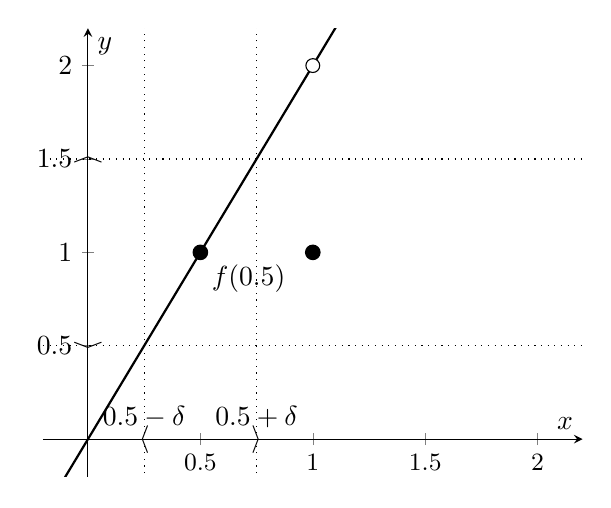
\begin{tikzpicture}
\begin{axis}[axis lines=middle,xlabel=$x$,ylabel=$y$, x tick label style = {font = \small},xmin=-0.2,xmax=2.2,ymin=-0.2,ymax=2.2]

\addplot[thick,color=black,domain=-1.5:3.5] {2*x};
\addplot[dotted,color=black,domain=-1.5:3.5] {0.5};
\addplot[dotted,color=black,domain=-1.5:3.5] {1.5};
\draw[dotted, color=black] (0.25, -1) -- (0.25, 2.5);
\draw[dotted, color=black] (0.75, -1) -- (0.75, 2.5);

\node[circle,draw=black, fill=white, inner sep=0pt,minimum size=5pt] at (1, 2) {};

\node at (axis cs:0.25,0) {$\langle$};
\node at (axis cs:0.75,0) {$\rangle$};
\node[label={[label distance=-0.1cm]-60:$f(0.5)$}] at (axis cs:0.5,1) {};
\node[label={[label distance=-0.1cm]90:$0.5+\delta$}] at (axis cs:0.75,0) {};
\node[label={[label distance=-0.1cm]90:$0.5-\delta$}] at (axis cs:0.25,0) {};
\node[circle,fill,inner sep=2pt] at (axis cs:1, 1) {};
\node[circle,fill,inner sep=2pt] at (axis cs:0.5, 1) {};
\node[rotate=90] at (axis cs:0,0.5) {$\langle$};
\node[rotate=90] at (axis cs:0,1.5) {$\rangle$};
\end{axis}
\end{tikzpicture}
\caption{Neprekidnost funkcije iz zadatka \ref{cont1} u $\frac{1}{2}$}
\end{subfigure}%
\begin{subfigure}[t]{.5\textwidth}
\centering
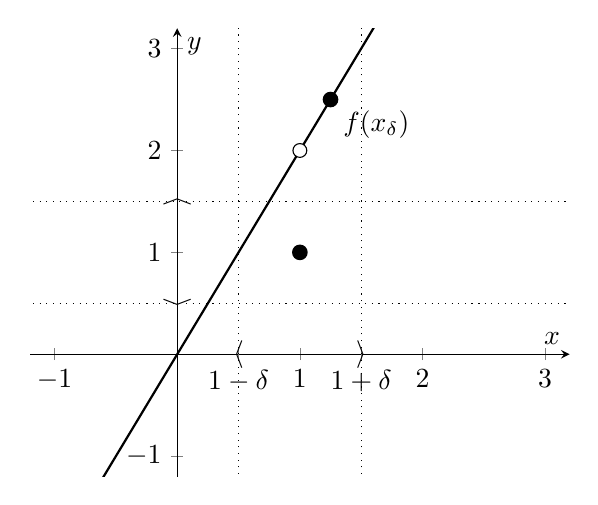
\begin{tikzpicture}
\begin{axis}[axis lines=middle,xlabel=$x$,ylabel=$y$, extra x ticks={0.5, 1.5}, extra x tick labels={$1-\delta$, $1+\delta$},xmin=-1.2,xmax=3.2,ymin=-1.2,ymax=3.2]

\addplot[thick,color=black,domain=-1.5:3.5] {2*x};
\addplot[dotted,color=black,domain=-1.5:3.5] {0.5};
\addplot[dotted,color=black,domain=-1.5:3.5] {1.5};

\node[circle,draw=black, fill=white, inner sep=0pt,minimum size=5pt] at (1, 2) {};

\node at (axis cs:0.5,0) {$\langle$};
\node at (axis cs:1.5,0) {$\rangle$};
\node[label={[label distance=-0.1cm]-30:$f(x_\delta)$}] at (axis cs:1.25,2.5) {};
\node[circle,fill,inner sep=2pt] at (axis cs:1, 1) {};
\node[circle,fill,inner sep=2pt] at (axis cs:1.25, 2.5) {};
\node[rotate=90] at (axis cs:0,0.5) {$\langle$};
\node[rotate=90] at (axis cs:0,1.5) {$\rangle$};
\draw[dotted, color=black] (0.5, -1.5) -- (0.5, 3.5);
\draw[dotted, color=black] (1.5, -1.5) -- (1.5, 3.5);
\end{axis}
\end{tikzpicture}
\caption{Prekid funkcije iz zadatka \ref{cont1} u $1$}
\end{subfigure}
\end{figure}

Primijetimo da za sve $x\in \mathbb{R}$ vrijedi $f(x)=2x$ ako i samo ako je $x\neq 1$, pa moramo odabrati $\delta$ takav da interval $\langle c-\delta, c+\delta\rangle$ ne sadrži broj $1$. Zaista, neka je $\epsilon>0$ proizvoljan. Uzmemo li $$\delta=\min\left \{\dfrac{\epsilon}{2},\; \dfrac{|1-c|}{2}\right\},$$
vrijedi $1\notin \langle c-\delta, c+\delta\rangle$, pa za svaki $x\in \mathbb{R}$ za koji je $|x-c|<\delta$ je $$|2x-2c|=2|x-c|<2\cdot \dfrac{\epsilon}{2}=\epsilon.$$ 
Dokažimo sada da za $c=1$ funkcija ima prekid. Treba dokazati da postoji $\epsilon>0$ takav da za sve $\delta>0$ postoji $x_\delta\in \mathbb{R}$ takav da je 
$$|x_\delta-1|<\delta\;\;\text{ i }\;\;|f(x_\delta)-1|\geq \epsilon.$$ 
Uzmemo li $\epsilon=\dfrac{1}{2}$, $\delta>0$ proizvoljan i $x_\delta=1+\dfrac{\delta}{2}$, imamo 
$$|x_\delta-1|=\dfrac{\delta}{2}<\delta$$ 
i kako je $x_\delta> 1$, slijedi $f(x_\delta)=2x_\delta>2$, pa vrijedi $|f(x_\delta)-1|>1> \epsilon$.
\end{proof}
\begin{remark}
Primijetimo da za sve $x, c\in \mathbb{R}$ i $\delta>0$ takav da je $|x-c|<\delta$ imamo
\begin{gather*}
|c|=|c-x+x|\leq |x-c|+|x|<\delta+|x|,\\
|x|=|x-c+c|\leq |x-c|+|c|,
\end{gather*}
što daje
\begin{gather}
\label{42}
|x|>|c|-\delta,\\
\label{43}
|x|<\delta+|c|.
\end{gather}

\noindent (\ref{42}) daje donju među, a (\ref{43}) gornju među za $|x|$, stoga su ove dvije tvrdnje često korisne kada se treba izraza $|x|$ "riješiti" kako bismo mogli uzeti $\delta$ koji ne ovisi o $x$.
\end{remark}
\begin{exercise}
\label{cont2}
Dokažite sljedeće tvrdnje koristeći definiciju neprekidnosti funkcije.
\begin{itemize}
\item[a)] $f : \mathbb{R}\to \mathbb{R}$, $f(x)=x^2$ je neprekidna na $\mathbb{R}$.
\item[b)] $f : \mathbb{R}\setminus\{0\}\to \mathbb{R}$, $f(x)=\dfrac{1}{x^2}$ je neprekidna na svojoj domeni.
\end{itemize}
\end{exercise}
\begin{proof*}
a) Neka su $c\in \mathbb{R}$ i $\epsilon>0$ proizvoljni. Uzmimo $$\delta=\min\left\{\dfrac{\epsilon}{1+2|c|}, 1\right\}.$$ 
Tada za sve $x\in \mathbb{R}$ takve da je $|x-c|<\delta$ vrijedi 
\begin{gather*}
|x|=|x-c+c|\leq |x-c|+|c|\leq 1+|c|,\\
|x+c|\leq |x|+|c|\leq 1+2|c|.
\end{gather*}
Odavde slijedi
$$|x^2-c^2|=|x-c||x+c|<\dfrac{\epsilon}{1+2|c|}\cdot(1+2|c|)=\epsilon.$$
b) Neka su $c\in \mathbb{R}\setminus\{0\}$ i $\epsilon>0$ proizvoljni. Vrijedi
$$\abs{\dfrac{1}{x^2}-\dfrac{1}{c^2}}=\dfrac{|x^2-c^2|}{|x|^2|c|^2}=\dfrac{|x-c||x+c|}{x^2c^2}$$
Uzmimo
$$\delta=\min\left\{\dfrac{\epsilon\cdot c^4}{4\left(1+2|c|\right)}, 1, \dfrac{|c|}{2}\right\}.$$
Iz (\ref{42}) imamo $$|x|>|c|-\dfrac{|c|}{2}=\dfrac{|c|}{2},\; \text{ tj. }\; x^2>\dfrac{c^2}{4}.$$
Nadalje, kao i u a) dijelu zadatka imamo $|x|+|c|\leq 1+2|c|$. Sve skupa, imamo
\[
\pushQED{\qed}
\dfrac{|x^2-c^2|}{|x|^2|c|^2}=\dfrac{|x-c||x+c|}{x^2c^2}<\dfrac{4|x-c|(1+2|c|)}{c^4}<\epsilon.\qedhere
\popQED
\]
\end{proof*}
\begin{remark}
U b) dijelu zadatka \ref{cont2}, gornju među od $|x+c|$ mogli smo naći i na sljedeći način.

Ako je $c>0$, onda za neki $\delta\leq \dfrac{c}{2}$ imamo
$$|x-c|< \delta\leq \dfrac{c}{2} \Longrightarrow -\dfrac{c}{2}<x-c<\dfrac{c}{2},$$
odakle, zbog činjenice da je $x=|x|$ slijedi
\begin{gather}
\label{44}
\dfrac{c}{2}<|x|<\dfrac{3c}{2},\;\; \dfrac{3c}{2}<|x+c|<\dfrac{5c}{2},
\end{gather}
pa imamo gornju i donju među za $|x+c|$, ali i $|x|$.

Ako je $c<0$, za neki $\delta\leq -\dfrac{c}{2}$  dobivamo $\dfrac{c}{2}<x-c<-\dfrac{c}{2}$, odnosno 
\begin{gather*}
\dfrac{3c}{2}<x<\dfrac{c}{2},\;\; \dfrac{5c}{2}<x+c<\dfrac{3c}{2},
\end{gather*}
no kako je $x\mapsto |x|$ strogo padajuća na $\langle -\infty, 0\rangle$, dobivamo
\begin{gather*}
-\dfrac{c}{2}<|x|<-\dfrac{3c}{2},\;\; -\dfrac{3c}{2}<|x+c|<-\dfrac{5c}{2},
\end{gather*}
dakle opet imamo gornju i donju među za $|x+c|$ i $|x|$.
\end{remark}
\begin{exercise}
Dokažite koristeći definiciju neprekidnosti funkcije da je funkcija $f : \mathbb{R}\to\mathbb{R}$,
$$f(x)=\begin{cases}
-x, & x\in \mathbb{Q},\\
x, & x\in \mathbb{I},
\end{cases}$$
neprekidna u $0$ i ima prekid u svakoj drugoj točki.
\end{exercise}
\newpage
\begin{proof}[Rješenje]
Neka je $\epsilon>0$ proizvoljan. Tada za $\delta=\epsilon$ i za $x\in \mathbb{R}$ takve da je $|x|<\delta$ vrijedi $|f(x)|=|x|<\epsilon,$ čime smo dokazali neprekidnost u $0$.

Dokažimo da $f$ ima prekid u svakoj točki $c>0$. Pretpostavimo sada da je $f$ neprekidna za neki iracionalni $c>0$. Tada tvrdnja vrijedi i za $\epsilon=f(c)$, pa postoji $\delta>0$ takav da za sve $x\in \mathbb{R}$ za koje je $|x-c|<\delta$ vrijedi $|f(x)-f(c)|<f(c)$. Tada vrijedi $$f(x)-f(c)>-f(c),$$ odnosno $f(x)>0$ za sve $x$ za koje je $|x-c|<\delta$. No za $\delta$ zbog gustoće skupa $\mathbb{Q}$ u $\mathbb{R}$, postoji $x_\delta\in \mathbb{Q}$ takav da je $$|x_\delta-c|<\delta.$$ Kako je $x_\delta\in \mathbb{Q}$, vrijedi $f(x_\delta)\leq 0$, što je nemoguće. 

Tvrdnja se analogno dokazuje ako je $x$ racionalan i ako je $c<0$.
\end{proof}
\begin{exercise}
\label{cont4}
Dokažite sljedeće tvrdnje koristeći definiciju neprekidnosti funkcije. 
\begin{itemize}
\item[a)] $f : [0,\infty \rangle\to \mathbb{R}$, $f(x)=\sqrt{x}$ je neprekidna na svojoj domeni.
\item[b)] $f : \mathbb{R} \to \mathbb{R}$, $f(x)=\sin{x}$ je neprekidna na svojoj domeni.
\end{itemize}
\end{exercise}
\begin{proof*}
a) Neka je $\epsilon, c>0$ proizvoljni. Uzmemo li $\delta=\sqrt{c}\epsilon$, za sve $x\geq 0$ za koje je $|x-c|<\delta$ imamo
$$|\sqrt{x}-\sqrt{c}|=\abs{\left(\sqrt{x}-\sqrt{c}\right)\dfrac{\sqrt{x}+\sqrt{c}}{\sqrt{x}+\sqrt{c}}}=\dfrac{|x-c|}{\sqrt{x}+\sqrt{c}}<\dfrac{|x-c|}{\sqrt{c}}<\epsilon$$

b) Neka su $\epsilon>0$ i $c\in \mathbb{R}$ proizvoljni. Uzmemo li $\delta=\epsilon$, za sve $x\in \mathbb{R}$ za koje je $|x-c|<\delta$ vrijedi
$$\abs{\sin{x}-\sin{c}}=\abs{2\cos{\dfrac{x+c}{2}}\sin{\dfrac{x-c}{2}}}\leq 2\abs{\sin{\dfrac{x-c}{2}}},$$
gdje smo iskoristili činjenicu da je $\abs{\cos{\dfrac{x+c}{2}}}\leq 1$. Kako za sve $x\in \mathbb{R}$ vrijedi $\abs{\sin{\dfrac{x-c}{2}}}\leq \abs{\dfrac{x-c}{2}},$ imamo
\[
\pushQED{\qed}
2\abs{\sin{\dfrac{x-c}{2}}}\leq |x-c|<\epsilon.\qedhere
\popQED
\]
\end{proof*}
\newpage
\begin{exercise}
\label{cont3}
Koristeći definiciju neprekidnosti funkcije, odredite najveći\footnote{Najveći skup $S\subseteq \mathbb{R}$ takav da je $f$ neprekidna je skup sa svojstvom da za sve $T\subseteq \mathbb{R}$ za koje je $f$ neprekidna vrijedi $T\subseteq S$.} skup na kojem je funkcija $f : \mathbb{R}\to \mathbb{R}$,
$$f(x)=\begin{cases}
\sqrt{2x-1},& x\geq 1,\\
\dfrac{1}{2}-x,& x<1.
\end{cases}$$
neprekidna.
\end{exercise}
\begin{proof*}

Iz grafa funkcije $f$ vidimo da će ona biti neprekidna svugdje osim u točki $1$. Dokažimo prvo da je $f$ neprekidna na skupu $\mathbb{R}\setminus\{1\}$. 

Zaista, neka je $c>1$ i $$\delta=\min\left\{\dfrac{\sqrt{2c-1}}{2}\epsilon,\; c-1\right\}.$$
Tada za sve $x\in \mathbb{R}$, $|x-c|<c-1$ povlači $x>1$, stoga je 
$$f(x)=\sqrt{2x-1}\;\;\text{ i }\;\;f(c)=\sqrt{2c-1}.$$ 

Neka je $\epsilon>0$ proizvoljan. Slično kao u a) dijelu zadatka \ref{cont4}, za sve $x\in \mathbb{R}$ za koje je $|x-c|<\delta$ vrijedi
\begin{align*}
\abs{\left(\sqrt{2x-1}-\sqrt{2c-1}\right)\cdot\dfrac{\sqrt{2x-1}+\sqrt{2c-1}}{\sqrt{2x-1}+\sqrt{2c-1}}}&=\dfrac{\abs{(2x-1)-(2c-1)}}{\sqrt{2x-1}+\sqrt{2c-1}}\\
&=\dfrac{2|x-c|}{\sqrt{2x-1}+\sqrt{2c-1}}<\dfrac{2|x-c|}{\sqrt{2c-1}}<\epsilon.
\end{align*}

Neka je sada $c<1$ i
$$\delta=\min\left\{\epsilon,\; 1-c\right\}.$$
Dobivamo $|x-c|<1-c$, odakle slijedi $x<1$, pa je $$f(x)=\dfrac{1}{2}-x\;\;\text{ i }\;\;f(c)=\dfrac{1}{2}-c.$$ Neka je $\epsilon>0$ proizvoljan. Za sve $x\in \mathbb{R}$ takve da je $|x-c|<\delta$ vrijedi
$$\abs{\left(\dfrac{1}{2}-x\right)-\left(\dfrac{1}{2}-c\right)}=|x-c|<\epsilon.$$
\newpage
Pokažimo sada da funkcija ima prekid za $c=1$. Uzmimo $\epsilon=\dfrac{1}{2}$ i neka je $\delta>0$ proizvoljan. Uzmimo sada $x_\delta=\max\left\{0,\; 1-\dfrac{\delta}{2}\right\}$. Uočimo da vrijedi 
$$|x_\delta-1|\leq\dfrac{\delta}{2}<\delta.$$
Naime, ako je $1-\dfrac{\delta}{2}\geq 0$, to je jasno, a ako je $1-\dfrac{\delta}{2}\leq 0$, onda je $\delta\geq 2$ i $x_\delta=0$, pa je $$|x_\delta-1|=|0-1|=1\leq\dfrac{\delta}{2}.$$
Kako je $0\leq x_\delta<1$, slijedi $f(x_\delta)=\dfrac{1}{2}-x_\delta\in \left\langle -\dfrac{1}{2}, \dfrac{1}{2}\right]$. To povlači
\[
\pushQED{\qed}
|f(x_\delta)-1|\geq \dfrac{1}{2}=\epsilon.\qedhere
\popQED
\]
\begin{figure}[ht]
\begin{center}
\begin{tikzpicture}
\begin{axis}[axis lines=middle,xlabel=$x$,ylabel=$y$,xmin=-2,xmax=4,ymin=-1,ymax=2.5]

\addplot[thick,color=black,domain=1:4] {sqrt(2*x-1)};
\addplot[thick,color=black,domain=-3:1] {1/2-x};
\node[circle,draw=black, fill=white, inner sep=0pt,minimum size=5pt] at (1, -0.5) {};
\node[circle,fill,inner sep=2pt] at (axis cs:1, 1) {};
\end{axis}
\end{tikzpicture}
\end{center}
\caption{Graf funkcije iz zadatka \ref{cont3}}
\end{figure}
\end{proof*}
\section{Svojstva neprekidnih funkcija}
\begin{remark}[Neprekidnost kompozicije funkcija]
\label{compcont}
Neka su $I, I'\subseteq \mathbb{R}$ otvoreni intervali i $f : I\to \mathbb{R}$, $g : I'\to \mathbb{R}$ funkcije takve da je $f(I)\subseteq I'$. Neka je $f$ neprekidna u točki $c\in I$, a $g$ neprekidna u točki $d=f(c)\in I'$. Tada je $h=g\circ f$ neprekidna u točki $c$.
\end{remark}
\begin{remark}[Teorem o lokalnoj ograničenosti neprekidne funkcije]
\label{localbound}
Neka je $I\subseteq \mathbb{R}$ otvoreni interval, $c\in I$ i neka je $f : I\to \mathbb{R}$ neprekidna u $c$. Tada postoje realni brojevi $\eta>0$ i $M>0$ takvi da za sve $x\in I$ vrijedi
$$|x-c|<\eta\Longrightarrow |f(x)|<M.$$
\end{remark}
\begin{remark}[Osnovne operacije s neprekidnim funkcijama]
\label{fundamentalopcont}
Neka je $I\subseteq \mathbb{R}$ otvoreni interval, te neka su $f, g : I\to \mathbb{R}$ neprekidna u točki $c\in I$. Vrijedi:
\begin{itemize}
\item[a)] $f+g$ je neprekidna u $c$,
\item[b)] $fg$ je neprekidna u $c$,
\item[c)] Ako je $g(x)\neq 0$ za sve $x\in I$, onda je $\dfrac{f}{g}$ neprekidna u $c$,
\item[d)] $|f|$ je neprekidna u $c$.
\end{itemize}
\end{remark}
\begin{exercise}
Dokažite napomenu \ref{fundamentalopcont} koristeći definiciju neprekidnosti funkcije.
\end{exercise}
\begin{proof}
a) Budući da su $f$ i $g$ neprekidne u $c$, za svaki $\epsilon>0$ postoje $\delta_1, \delta_2>0$ takvi da za sve $x\in I$ vrijedi
$$|x-c|<\delta_1\Longrightarrow |f(x)-f(c)|<\dfrac{\epsilon}{2}\;\;\text{ i }\;\; |x-c|<\delta_2\Longrightarrow |g(x)-g(c)|<\dfrac{\epsilon}{2}$$
Uzmimo $\delta=\min\{\delta_1, \delta_2\}$. Tada za sve $x\in I$ za koje je $|x-c|<\delta$ vrijedi
\begin{align*}
|(f+g)(x)-(f+g)(c)|&=\abs{\left(f(x)+g(x)\right)-\left(f(c)+g(c)\right)}=\abs{f(x)-f(c)+g(x)-g(c)}\\
&\leq |f(x)-f(c)|+|g(x)-g(c)|<\dfrac{\epsilon}{2}+\dfrac{\epsilon}{2}=\epsilon.
\end{align*}
b) Prema napomeni \ref{localbound} postoje $\eta_1, \eta_2, M_1, M_2>0$ takvi da za sve $x\in I$ vrijedi
$$|x-c|<\eta_1\Longrightarrow |f(x)|<M_1\;\;\text{ i }\;\; |x-c|<\eta_2\Longrightarrow |g(x)|<M_2.$$
Sada za $\eta=\min\left\{\eta_1, \eta_2\right\}$ i $M=\max\left\{M_1, M_2\right\}$ imamo da za sve $x\in I$ takve da je $|x-c|<\eta$ vrijedi $|f(x)|, |g(x)|<M$. Nadalje, zbog neprekidnosti od $f$ i $g$, za svaki $\epsilon>0$ postoje $\delta_1, \delta_2>0$ takvi da za sve $x\in I$ vrijedi
$$|x-c|<\delta_1\Longrightarrow |f(x)-f(c)|<\dfrac{\epsilon}{2M}\;\;\text{ i }\;\; |x-c|<\delta_2\Longrightarrow |g(x)-g(c)|<\dfrac{\epsilon}{2M}.$$
Uzmimo $\delta=\min\{\delta_1, \delta_2, \eta\}$. Tada je
\begin{align*}
|(fg)(x)-(fg)(c)|&=\abs{f(x)g(x)-f(c)g(c)}\\
&=\abs{f(x)g(x)-f(c)g(x)+f(c)g(x)-f(c)g(c)}\\
&\leq |f(x)-f(c)||g(x)|+|g(x)-g(c)||f(c)|<\dfrac{\epsilon}{2M}\cdot M+\dfrac{\epsilon}{2M}\cdot M=\epsilon.
\end{align*}
c) Nije teško pokazati da je funkcije $q : I\setminus\{0\}\to \mathbb{R}$, $q(x)=\dfrac{1}{x}$ neprekidna na svojoj domeni. Uočimo da je $\dfrac{1}{g}=q\circ g$. Za sve $c\in I\setminus\{0\}$ vrijedi $g(c)\neq 0$, pa je, po napomeni \ref{compcont} i $\dfrac{1}{g}=q\circ g$ neprekidna u $c$. No i $f$ je neprekidna u $c$, pa je prema b), $f\cdot \dfrac{1}{g}=\dfrac{f}{g}$ neprekidna u $c$, dakle i neprekidna na $I\setminus\{0\}$.

d) Lako je pokazati da je $q : \mathbb{R}\to \mathbb{R}$, $q(x)=|x|$ neprekidna na $\mathbb{I}$. Kako je $f$ neprekidna na $\mathbb{R}$, slijedi i da je $q\circ f=|f|$ neprekidna na $\mathbb{R}$.
\end{proof}
\begin{remark}[Heineova karakterizacija neprekidnosti]
Neka je $I\subseteq \mathbb{R}$ otvoreni interval i neka je zadana $f : I\to \mathbb{R}$. Funkcija $f$ je neprekidna u točki $c\in I$ ako i samo ako za svaki niz $(a_n)$ iz $I$ koji konvergira prema $c$, niz $\left(f(a_n)\right)$ konvergira prema $f(c)$.
\end{remark}

Prethodna činjenica je vrlo korisna kako bi pokazali da neka funkcija ima prekid u nekoj točki.
\begin{exercise} Dokažite: Funkcija $f : \mathbb{R}\to \mathbb{R}$, $$f(x)=\begin{cases}
2x-1,\; x\leq 3,\\
-x+6,\; x>3.
\end{cases}$$
ima prekid u točki $c=3$.
\end{exercise}
\begin{proof}[Rješenje]
Dovoljno je pokazati da postoji niz $(a_n)$ realnih brojeva koji konvergira u $3$ takav da $\left(f(a_n)\right)$ ne konvergira u $f(3)=5$. Promotrimo niz $(a_n)$ zadan formulom $a_n=3+\dfrac{1}{n}$. Tada je $\lim\limits_{n\to \infty}{a_n}=3$, te kako je $a_n>3$ za sve $n\in \mathbb{N}$, za niz $\left(f(a_n)\right)$, gdje je
$$f(a_n)=-\left(\dfrac{1}{n}+3\right)+6=9-\dfrac{1}{n}$$
vrijedi $\lim\limits_{n\to \infty}{f(a_n)}=9\neq 5$, što je i trebalo pokazati.
\end{proof}
\begin{exercise}
Zadana je funkcija $f : \mathbb{R}\to \mathbb{R}$,
$$f(x)=\begin{cases}
-2, & x<0,\\
1, & x\geq 0.
\end{cases}$$
Dokažite da je ona neprekidna u svakoj točki $c\neq 0$ koristeći Heineovu karakterizaciju neprekidnosti.
\end{exercise}
\begin{proof}
Uzmimo npr. da je $c>0$, slučaj $c<0$ tretira se analogno. Uzmimo proizvoljan niz $(a_n)$ takav da je $\lim\limits_{n\to \infty}{a_n}=c$. Iz definicije slijedi da postoji $n_0\in \mathbb{R}$ takav da za sve prirodne $n\geq n_0$ vrijedi $|a_n-c|<c$, odakle slijedi da je $a_n>0$ za sve $n\geq n_0$. Zato je $f(a_n)=1=f(c)$ za sve $n\in \mathbb{N}$ osim za njih konačno mnogo, pa je jasno da je $\lim\limits_{n\to \infty}{a_n}=1$.
\end{proof}

\begin{exercise}
Zadana je funkcija $f : [0, 1]\to \mathbb{R}$, $$f(x)=\begin{cases}
1, \; x=0,\\
\dfrac{1}{n},\; x=\dfrac{m}{n}\in \mathbb{Q}\setminus\{0\},\mathrm{gdje\;su\;}m\in \mathbb{Z}\mathrm{\;i\;}n\in \mathbb{N}\mathrm{\;relativno\;prosti.}\\
0,\; x\in \mathbb{I}.
\end{cases}$$
Ova funkcija zove se \textit{Thomaeova funkcija}. Dokažite da je ona neprekidna u svakoj iracionalnoj točki i ima prekid u svakoj racionalnoj točki.
\end{exercise}
\begin{proof}[Rješenje]
Dokažimo sljedeću pomoćnu tvrdnju: Neka je $M>0$ proizvoljan. Tada je skup
$$S_M=\left\{x\in[0, 1] : f(x)\geq M\right\}$$
konačan. 

Zaista, ako je $M>1$, vrijedi $S_M=\emptyset$. 

Ako je $M\leq 1$, iz $f(x)\geq M>0$ slijedi da je ili $x=1$ (pa je $S_M$ konačan) ili postoji $n\in \mathbb{N}$ takav da je $f(x)=\dfrac{1}{n}$. Uočimo da je $$\dfrac{1}{n}\geq M\Longleftrightarrow n\leq \dfrac{1}{M},$$ pa je $\left\{n\in \mathbb{N} : \dfrac{1}{n}\geq M\right\}$ odozgo ograničen podskup skupa $\mathbb{N}$, dakle on je konačan. To znači da za sve $x\in S_M$ vrijedi ili $x=0$, ili postoje $m\in \mathbb{Z}$ i $n\in \mathbb{N}$ takvi da je $x=\dfrac{m}{n}$, kojih je očito konačno mnogo, jer je $n\in \left\{1, 2,\dots, \dfrac{1}{M}\right\}$, te $m\in \{1, \dots, n\}$.

Pokažimo sada neprekidnost funkcije u svakoj iracionalnoj točki. Neka su $\epsilon>0$ i $c\in \mathbb{I}$ proizvoljni. Tvrdimo da postoji $\delta>0$ takav da za sve $x\in \mathbb{R}$ vrijedi $$|x-c|<\delta\Rightarrow |f(x)|=f(x)<\epsilon.$$ 
Ako je $\epsilon\geq 1$, tvrdnja je trivijalna. Uzmimo zato $\epsilon<1$. Očito je tada skup $S_\epsilon$ neprazan, jer je npr. $0\in S_\epsilon$.

Neka je $x_0\in S_\epsilon$ točka takva da za sve $y\in S_\epsilon$ vrijedi $|x_0-c|\leq|y-c|$. Takva točka postoji, jer inače bi slično kao u rješenju zadatka \ref{limitpoints3} dobili da je $S_\epsilon$ beskonačan, što očito ne vrijedi. Tvrdimo da za $\delta=|x_0-c|$, ne postoji $x\in \mathbb{R}$ takav da je $|x-c|<\delta$ i $x\in S_\epsilon$. Zaista, u tom slučaju bi imali $$|x_0-c|\leq |x-c|<\delta=|x_0-c|,$$ kontradikcija! Ovo povlači da za sve $x\in \mathbb{R}$ takve da je $|x-c|<\delta$ vrijedi $|f(x)|<\epsilon$, što je i trebalo pokazati.

Dokažimo sada da funkcija ima prekid u svakoj racionalnoj točki. Zaista, ako je $q\in \mathbb{Q}$, onda je $f(q)\neq 0$, a kako za svaki broj $q$ postoji niz $(a_n)$ iracionalnih brojeva koji konvergira prema $q$ (Dokažite to!), za taj niz je $\lim\limits_{x\to \infty}{f(a_n)}=0\neq f(q)$, čime smo dokazali tvrdnju.
\end{proof}
\begin{remark}[Bolzano-Weierstrassov teorem]
Neka je $f : [a, b]\to \mathbb{R}$ neprekidna funkcija na segmentu $[a, b]$. Tada je $f([a, b])$ također segment.
\end{remark}
\begin{remark}
Neka je $f : [a, b]\to \mathbb{R}$ neprekidna funkcija na segmentu $[a, b]$. Prethodni teorem je ekvivalentan s konjunkcijom sljedeće tri tvrdnje.
\begin{itemize}
\item $f$ je ograničena na $[a, b]$, tj. postoji $M\in \mathbb{R}$ takav da je $|f(x)|\leq M$ za sve $x\in [a, b]$.
\item $f$ dostiže svoj infimum i supremum na $[a, b]$, tj. postoje $x_m, x_M\in [a, b]$ za koje je\footnote{Ako je $S\neq \emptyset$ i $f : S\to \mathbb{R}$, onda se $\inf{f}, \sup{f}, \min{f}, \max{f}$ definiraju kao $\inf{\mathcal{R}(f)}, \sup{\mathcal{R}(f)}, \min{\mathcal{R}(f)}, \max{\mathcal{R}(f)}$, respektivno.} 
\begin{gather*}
f(x_m)=\inf{f}=\min{f}=m,\\
f(x_M)=\sup{f}=\max{f}=M.
\end{gather*}
\item (Teorem o međuvrijednostima) Za svaki $C\in [m, M]$ postoji $c\in [a, b]$ takav da je $C=f(c)$.
\end{itemize}
\end{remark}
\newpage
\begin{exercise}
\label{imgcont1}
Zadana je $f : [0, 2]\to \mathbb{R}$, $f(x)=x^5+3x^3$. Odredite $\mathcal{R}(f)$.
\end{exercise}
\begin{proof}[Rješenje]
Uočimo da su $f_1 : [0, 2]\to \mathbb{R}$, $f(x)=x^5$ i $f_2 : [0, 2]\to \mathbb{R}$, $f_2(x)=3x^3$ strogo rastuće, pa je i $f=f_1+f_2$ strogo rastuća. Zato je $$f(0)=0=\min{f}\;\;\text{ i }\;\;f(2)=56=\max{f},$$
pa je $\mathcal{R}(f)\subseteq [0, 56]$.

S druge strane, može se pokazati da je $x\mapsto x^n$ je neprekidna na $\mathbb{R}$ za sve $n\in \mathbb{N}$ (v. \cite{3}), odakle slijedi i da je $f$ neprekidna na $\mathbb{R}$, te je specijalno $f$ neprekidna na $[0, 2]$. Iz teorema o međuvrijednostima imamo da za sve $C\in [0, 56]$ postoji $c\in [0, 2]$ takav da je $C=f(c)$. Odavde slijedi $[0, 56]\subseteq \mathcal{R}(f)$, pa je $\mathcal{R}(f)=[0, 56]$.
\end{proof}
\begin{exercise}
Zadana je $f : \mathbb{R}\to \mathbb{R}$, $f(x)=x\sin{x}$. Odredite $\mathcal{R}(f)$.
\end{exercise}
\begin{proof}[Rješenje]
Neka je $n\in \mathbb{N}$ proizvoljan. Kako je $f$ neprekidna na $\mathbb{R}$, ona je i neprekidna na segmentu $\left[-\dfrac{\pi}{2}-2n\pi, \dfrac{\pi}{2}+2n\pi\right]$. Uočimo da za sve $x\in \left[-\dfrac{\pi}{2}-2n\pi, \dfrac{\pi}{2}+2n\pi\right]$ vrijedi 
$$|x\sin{x}|=|x||\sin{x}|\leq |x|\leq \dfrac{\pi}{2}+2n\pi$$
i vrijedi $f\left(\dfrac{\pi}{2}+2n\pi\right)=\dfrac{\pi}{2}+2n\pi$, pa je $$\min{f}=-\dfrac{\pi}{2}-2n\pi\;\;\text{ i }\;\;\max{f}=\dfrac{\pi}{2}+2n\pi.$$
Odavde, slično kao u zadatku \ref{imgcont1}, slijedi $$f\left(\left[-\dfrac{\pi}{2}-2n\pi, \dfrac{\pi}{2}+2n\pi\right]\right)=\left[-\dfrac{\pi}{2}-2n\pi, \dfrac{\pi}{2}+2n\pi\right].$$
Neka je sada $y\in \mathbb{R}$ proizvoljan. Prema Arhimedovu aksiomu postoje $n_0, m_0\in \mathbb{N}$ takav da je 
$$n_0>\dfrac{y-\dfrac{\pi}{2}}{2}\;\;\text{ i }\;\; m_0>-\dfrac{y+\dfrac{\pi}{2}}{2\pi},$$
odnosno
$$\dfrac{\pi}{2}+2n_0\pi>y\;\;\text{ i }\;\;-\dfrac{\pi}{2}-2m_0\pi<y,$$
odakle za $n_1=\max\{n_0, m_0\}$ slijedi da je $y\in \left[-\dfrac{\pi}{2}-2n_1\pi, \dfrac{\pi}{2}+2n_1\pi\right]$. Međutim, kako je $f$ neprekidna na $\left[-\dfrac{\pi}{2}-2n_1\pi, \dfrac{\pi}{2}+2n_1\pi\right]$, postoji $x\in \mathbb{R}$ takav da je $y=f(x)$. Dakle, vrijedi $\mathbb{R}\subseteq \mathcal{R}(f)$, što znači da je $\mathcal{R}(f)=\mathbb{R}$.
\end{proof}
\begin{exercise}
Neka je $I\subseteq \mathbb{R}$ otvoreni interval i neka je $f : I\to \mathbb{R}$ neprekidna i strogo monotona na $I$. Dokažite da je tada $\mathcal{R}(f)$ otvoreni interval.
\end{exercise}
\begin{proof}
Uzmimo da $f$ strogo raste na $I$ (Analogno se tretira slučaj gdje $f$ strogo pada). Pretpostavimo da je $\inf{\mathcal{R}(f)}=\inf{f}\in \mathcal{R}(f)$. Tada postoji $a\in I$ takav da je $f(a)=\inf{f}$. Međutim, kako je $I$ otvoreni interval, postoji $a'\in I$ takav da je $a'<a$. Odavde je $f(a_1)\in \mathcal{R}(f)$ i vrijedi $f(a_1)<f(a)=\inf{f}$, kontradikcija! Analogno se pokazuje da $\sup{f}\notin \mathcal{R}(f)$. Odavde dobivamo $\mathcal{R}(f)\subseteq \langle \inf{f}, \sup{f} \rangle$.

Neka je $z\in \langle \inf{f}, \sup{f} \rangle$. Tada postoje $x, y\in \langle \inf{f}, \sup{f} \rangle$ takvi da je $x<z<y$. Kako je $f$ strogo rastuća, ona ima inverznu funkciju $f^{-1}$ koja je također strogo rastuća, pa je $f^{-1}(x)<f^{-1}(z)<f^{-1}(y)$. No tada je $f\left(\left[f^{-1}(x), f^{-1}(y)\right]\right)$ segment, pa je $$z\in f\left(\left[f^{-1}(x), f^{-1}(y)\right]\right)\;\;\text{ i }\;\;f\left(\left[f^{-1}(x), f^{-1}(y)\right]\right)\subseteq f(I)=\mathcal{R}(f),$$
što vrijedi zbog činjenice da za svaku funkciju $g : S\to \mathbb{R}$ i skupove $A\subseteq B\subseteq S$ vrijedi $f(A)\subseteq f(B)$ (Dokažite to!).
Dobivamo $z\in \mathcal{R}(f)$, pa zaključujemo da je $\mathcal{R}(f)=\langle \inf{f}, \sup{f}\rangle$.
\textbf{NADOPUNITI SLUCAJ KAD SLIKA NIJE OGRANICEN SKUP}
\end{proof}

\newpage
\section*{Zadatci za vježbu}
\subsection*{Definicija neprekidnosti funkcije}
\begin{exercise}
Koristeći definiciju neprekidnosti funkcije, dokažite sljedeće tvrdnje: 
\begin{itemize}
\item[a)] $x\mapsto |3x+2|$ je neprekidna na $\mathbb{R}$,
\item[b)] $x\mapsto x(x+1)$ je neprekidna na $\mathbb{R}$,
\item[c)] $x\mapsto x^3$ je neprekidna na $\mathbb{R}$,
\item[d)] $x\mapsto \dfrac{1}{\sqrt{x}}$ je neprekidna na $\mathbb{R}^+$,
\item[e)] $x\mapsto \sqrt{x^2+1}$ je neprekidna u $0$,
\item[f)] $f : \mathbb{R}\to \mathbb{R}$, $$f(x)=\begin{cases}
x\sin{\dfrac{1}{x}}, & x\neq 0,\\
0, & x=0,
\end{cases}
$$ 
je neprekidna u $0$,
\item[g)] $x\mapsto 2\sin^2{x}-1$ je neprekidna na $\mathbb{R}$.
\end{itemize}
\end{exercise}
\begin{exercise}
Zadan je otvoreni interval $I\subseteq \mathbb{R}$ i funkcija $f : I\to \mathbb{R}$. Dokažite ili opovrgnite: $f$ je neprekidna u $c$ ako i samo ako...
\begin{itemize}
\item[a)] Postoji $\delta>0$ takav da za sve $\epsilon>0$ i sve $x\in I$ vrijedi $|x-c|<\delta\Rightarrow |f(x)-f(c)|<\epsilon$,
\item[b)] Za svaki $\epsilon>0$ postoji $\delta>0$ takav da za sve $x\in I$ vrijedi $|f(x)-f(c)|<\epsilon\Rightarrow |x-c|<\delta$,
\item[c)] Za svaki $\delta>0$ postoji $\epsilon>0$ takav da za sve $x\in I$ vrijedi $|x-c|<\delta\Rightarrow |f(x)-f(c)|<\epsilon$.
\end{itemize}
\end{exercise}
\begin{exercise}
Neka je $I\subseteq \mathbb{R}$ otvoreni interval i $c\in I$. Zadana je funkcija $f : I\to \mathbb{R}$ sa sljedećim svojstvom: Za svaki $k\in \mathbb{N}$ postoji $\delta>0$ tako da za sve $x\in I$ vrijedi $|x-c|<\delta\Rightarrow |f(x)-f(c)|<\dfrac{1}{2^k}$. Dokažite ili opovrgnite: $f$ je neprekidna u $c$.
\end{exercise}
\begin{exercise}
Koristeći definiciju neprekidnosti funkcije, odredite najveći skup na kojem je funkcija $f : \mathbb{R}\to \mathbb{R}$,
$$f(x)=\begin{cases}
x^2,& x\leq 3,\\
2x+1,& x>3.
\end{cases}$$
neprekidna.
\end{exercise}
\begin{exercise} $(*)$
Koristeći definiciju neprekidnosti funkcije, dokažite da je $\sqrt[3]{x}$ neprekidna na svojoj domeni.
\end{exercise}
\subsection*{Svojstva neprekidnih funkcija}
\begin{exercise}
Postoji li $c\in \mathbb{R}$ takav da vrijedi:
\begin{itemize}
\item[a)] $f : \mathbb{R}\to \mathbb{R}$, $$f(x)=\begin{cases}
\arctg{\dfrac{1}{x-1}},& x\neq 1,\\
c, & x=1
\end{cases}$$ 
je neprekidna u $1$.
\item[b)] Funkcija $f : \mathbb{R}\to \mathbb{R}$, $$f(x)=\begin{cases}
2x-c,& x\leq 1,\\
\sqrt{x-1},& x>1.
\end{cases}$$
je neprekidna u $1$.
\item[b)] $f : \mathbb{R}\to \mathbb{R}$, $$f(x)=\begin{cases}
\sin{\dfrac{1}{x}},\; x\neq 0,\\
c,\; x=0.
\end{cases}$$
je neprekidna u $0$.
\end{itemize}
\end{exercise}
\begin{exercise}
Dokažite da je $\mathcal{R}(\sin)=\mathcal{R}(\cos)=[-1, 1]$ i da je $\mathcal{R}(\tg)=\mathbb{R}$.
\end{exercise}

\begin{thebibliography}{9}
\bibitem{1}
M. Vuković, \textit{Matematička logika}, skripta, PMF -- Matematički odsjek, Zagreb, 2007.
\bibitem{2}
K. Horvatić, \textit{Linearna algebra}, Golden marketing -- Tehnička knjiga, Zagreb, 2004.
\bibitem{3}
D. Krizmanić, \textit{Matematička analiza 1}, skripta, Fakultet za matematiku Sveučilišta u Rijeci, Rijeka, 2024.
\bibitem{4}
A. Dujella, \textit{Teorija brojeva}, Školska knjiga, Zagreb, 2019.
\bibitem{5}
S. Kurepa, \textit{Matematička analiza 1}, Školska knjiga, Zagreb, 1976.
\bibitem{6}
\textit{Applying the Arithmetic Mean Geometric Mean Inequality}. Brilliant.org. Preuzeto u 11:12, 19. srpnja 2024., \href{https://brilliant.org/wiki/applying-the-arithmetic-mean-geometric-mean/}{Za link kliknite ovdje}.
\bibitem{7}
\textit{Arithmetic Mean - Geometric Mean}. Brilliant.org. Preuzeto u 15:54, 19. srpnja 2024., \href{https://brilliant.org/wiki/arithmetic-mean-geometric-mean/}{Za link kliknite ovdje}.
\bibitem{8}
B. P. Demidovič i suradnici, \textit{Zadaci i riješeni primjeri iz matematičke analize za tehničke fakultete}, Sedmo ispravljeno izdanje, Golden marketing, Zagreb, 2003.
\bibitem{9} S. Mardešić, \textit{Matematička analiza u $n$-dimenzionalnom realnom prostoru}, Prvi dio, Školska knjiga, Zagreb, 1974.
\bibitem{10} Grupa autora, \foreignlanguage{russian}{Spravočnoe posobie po matematičeskomu analizu, Prvi dio, Višča škola, Kijev, 1978.}
\bibitem{11} M. Vuković, \textit{Teorija skupova}, predavanja, PMF -- Matematički odsjek, Zagreb, 2015.
\bibitem{12} B. Pavković, D. Veljan, \textit{Elementarna matematika 1}, Školska knjiga, Zagreb, 2004.
\bibitem{13} T.-L. Radulescu, V. D. Radulescu, T. Andreescu, \textit{Problems in Real Analysis: Advanced Calculus on the Real Axis}, Springer, 2009.
\bibitem{14} S. Kurepa, \textit{Matematička analiza 2}, Školska knjiga, Zagreb, 1997.
\end{thebibliography}

\end{document}
